% -=-=-=-=-=-=-=-=-=-=-=-=-=-=-=-=-=-=-=-=-=-=-=-=-=-=-=-=-=-=-=-=-=-=-=-=-=-=-=
% COURS MUI
% Bertrand Hochet  Pierre Favrat  C�dric Bornand
% created February 2016
% version 
% -=-=-=-=-=-=-=-=-=-=-=-=-=-=-=-=-=-=-=-=-=-=-=-=-=-=-=-=-=-=-=-=-=-=-=-=-=-=-=
\documentclass[10pt,a4paper]{book}
\usepackage[latin1]{inputenc}
\usepackage[T1]{fontenc}
\usepackage[english,english,french]{babel}

%\usepackage[utf8]{inputenc}
\usepackage[french]{babel}
% -=-=-=-=-=-=-=-=-=-=-=-=-=-=-=-=-=-=-=-=-=-=-=-=-=-=-=-=-=-=-=-=-=-=-=-=-=-=-=
% 
% 
%
% -=-=-=-=-=-=-=-=-=-=-=-=-=-=-=-=-=-=-=-=-=-=-=-=-=-=-=-=-=-=-=-=-=-=-=-=-=-=-=


% divers packages utiles
\usepackage{enumitem}
\usepackage{graphicx}
\usepackage{ifthen}
\usepackage{amssymb}
\usepackage{chngpage}
\usepackage{lastpage}
\usepackage{listings}
\usepackage{amsmath}
\usepackage{amssymb,amsfonts,textcomp}
\usepackage{color}
\usepackage{colortbl}
\usepackage{xcolor}
\usepackage{amssymb}
%\usepackage{algorithm,algorithmic}
\usepackage{algorithmic}
\usepackage{algorithm}
\usepackage{array}
\usepackage{supertabular}
\usepackage{multirow} 
\usepackage{hhline}
\usepackage{hyperref}
%\usepackage{tikz}
\hypersetup{pdftex, colorlinks=true, linkcolor=blue, citecolor=blue, filecolor=blue, urlcolor=blue, pdftitle=microinformatique, pdfauthor=linuxmint , pdfsubject=Chapitre 01 - Introduction, pdfkeywords=}
\usepackage{fancyhdr}
\usepackage{chappg}

% taille imprimable
\usepackage{fullpage} % Agrandit les dimensions du texte (hauteur, largeur,
                     % etc.) par rapport  celles par dfaut. Attention
                     % ce package ne se trouve pas dans toutes les
                     % distributions LaTeX

% -=-=-=-=-=-=-=-=-=-=-=-=-=-=-=-=-=-=-=-=-=-=-=-=-=-=-=-=-=-=-=-=-=-=-=-=-=-=-=
\usepackage[a4paper, top=1cm, bottom=2.5cm, left=2cm, headheight=6mm, headsep=5mm, marginparwidth=0.5cm, marginparsep=4mm, heightrounded, includehead]{geometry} 

% -=-=-=-=-=-=-=-=-=-=-=-=-=-=-=-=-=-=-=-=-=-=-=-=-=-=-=-=-=-=-=-=-=-=-=-=-=-=-=
 
%
\newcommand\textstyleInternetlink[1]{\textcolor{blue}{#1}}

%\newcommand\textsubscript[1]{\ensuremath{{}_{\text{#1}}}}
\makeatletter
\newcommand\arraybslash{\let\\\@arraycr}
\makeatother
% Footnote rule
\setlength{\skip\footins}{0.119cm}
\renewcommand\footnoterule{\vspace*{-0.018cm}\setlength\leftskip{0pt}\setlength\rightskip{0pt plus 1fil}\noindent\textcolor{black}{\rule{0.25\columnwidth}{0.018cm}}\vspace*{0.101cm}}
% Pages styles
\makeatletter
\newcommand\ps@Standard{
  \renewcommand\@oddhead{}
  \renewcommand\@evenhead{\@oddhead}
  \renewcommand\@oddfoot{}
  \renewcommand\@evenfoot{}
  \renewcommand\thepage{\arabic{page}}
}
\makeatother
\pagestyle{Standard}
\setlength\tabcolsep{1mm}
\renewcommand\arraystretch{1.3}
\newcounter{Figure}
\renewcommand\theFigure{\arabic{Figure}}
\newcounter{quation}
\renewcommand\thequation{\arabic{quation}}
\newcounter{Table}
\renewcommand\theTable{\arabic{Table}}

\newcommand\normalsubformula[1]{\text{\mathversion{normal}$#1$}}


%%%%%%%%%%%%%%%%%%%%%%%%%%%%%% Textclass specific LaTeX commands.
\newenvironment{lyxcode}
{\par\begin{list}{}{
\setlength{\rightmargin}{\leftmargin}
\setlength{\listparindent}{0pt}% needed for AMS classes
\raggedright
\setlength{\itemsep}{0pt}
\setlength{\parsep}{0pt}
\normalfont\ttfamily}%
 \item[]}
{\end{list}}


% -=-=-=-=-=-=-=-=-=-=-=-=-=-=-=-=-=-=-=-=-=-=-=-=-=-=-=-=-=-=-=-=-=-=-=-=-=-=-=
% donnes pour le titre
\title{MUI - Microinformatique }
\author{Cours cr�� par C�dric Bornand, Pierre Favrat et Bertrand Hochet\\ \\  HEIG-VD}

\newcommand{\version}{0.4}
\newcommand{\dateversion}{01.02.2017}

\date{R�vision \version\ - Mise � jour du \dateversion}
% -=-=-=-=-=-=-=-=-=-=-=-=-=-=-=-=-=-=-=-=-=-=-=-=-=-=-=-=-=-=-=-=-=-=-=-=-=-=-=
% CORPS DU DOCUMENT
% -=-=-=-=-=-=-=-=-=-=-=-=-=-=-=-=-=-=-=-=-=-=-=-=-=-=-=-=-=-=-=-=-=-=-=-=-=-=-=

\begin{document}

%definition zone listing
\definecolor{gris}{rgb}{0.95,0.95,0.95}
\lstset{numbers=none, tabsize=4, backgroundcolor=\color{gris}, frame=single, breaklines=true, showlines=true, keywordstyle=\color{black}, stringstyle=\ttfamily, framexleftmargin=6mm, xleftmargin=6mm}

\newcommand{\lstnormal}{\lstset{numbers=none, tabsize=4, backgroundcolor=\color{gris},frame=single, breaklines=true, showlines=true,keywordstyle=\color{black},stringstyle=\ttfamily,framexleftmargin=6mm, xleftmargin=6mm}}

\newcommand{\lstfondblanc}{\lstset{numbers=none, tabsize=4, backgroundcolor=\color{white},frame=none, breaklines=true, showlines=true, keywordstyle=\color{black},stringstyle=\ttfamily,framexleftmargin=6mm, xleftmargin=6mm} }

\lstdefinestyle{customc}{
  belowcaptionskip=1\baselineskip,
  breaklines=true,
  frame=L,
  xleftmargin=\parindent,
  language=C,
  showstringspaces=false,
  basicstyle=\footnotesize\ttfamily,
  keywordstyle=\bfseries\color{green!40!black},
  commentstyle=\itshape\color{purple!40!black},
  identifierstyle=\color{blue},
  stringstyle=\color{orange},
  extendedchars=true,
  basicstyle=\fontfamily{pcr}\selectfont
}

\newcommand{\be}{\begin{enumerate}}

\setcounter{secnumdepth}{3} % profondeur de numerotation max 0.0.0.0
\setcounter{tocdepth}{3} % profondeur titres table des mati�res

\pagestyle{fancy}
\fancyhead{}

\renewcommand{\chaptermark}[1]%
{\markboth{\MakeUppercase{\thechapter.\ #1}}{}}

\fancyhf{} 
\fancyhead[LE,LO]{}
\fancyhead[LE,RO]{Cours MUI - r\version\ - \dateversion}
\renewcommand{\headrulewidth}{1pt}
\renewcommand{\footrulewidth}{1pt}
\fancyfoot[RE,LO]{HEIG-VD / C�dric Bornand, Pierre Favrat et Bertrand Hochet}
\fancyfoot[LE,RO]{Page \thepage}

% redfini le style pour plain (1re page des chapitres)

\fancypagestyle{plain}{%
  \fancyfoot[RE,LO]{HEIG-VD / MUI/ C�dric Bornand, Pierre Favrat et Bertrand Hochet}
  \fancyfoot[LE,RO]{Page \thepage}
  \fancyhead[LE,RO]{}
 \renewcommand{\headrulewidth}{1pt}
  \renewcommand{\footrulewidth}{1pt}
}

% redfini le style pour empty (pour la page de titre)
\fancypagestyle{empty}{%
  \fancyfoot[RE,LO]{}
  \fancyfoot[LE,RO]{}
%  \fancyhead[LE,RO]{}
  \fancyhead[LE,RO]{
\includegraphics[scale=0.5,angle=0]{logo_HEIG_VD.png}}
  \renewcommand{\headrulewidth}{0pt}
  \renewcommand{\footrulewidth}{0pt}
}

\begin{titlepage}
\begin{tabular}{l}
 \\
 \\
 \\
 \\
 \\
 \\
 \\

\end{tabular}
\begin{center}
\Large\textbf{\textsc{Cours -  Microinformatique} }\\

\Large\textbf{ (MUI)}
\end{center}
\begin{tabular}{c}
 \\
 \\
\end{tabular}
\begin{center}
\textbf{Cours cr�� par C�dric Bornand, Pierre Favrat et Bertrand Hochet}
\end{center}
\begin{center}
\textbf{HEIG-VD}
\textbf{mars 2017} \\
 rev. \version
\end{center}
\begin{tabular}{c}
 \\ 
\end{tabular}

 \end{titlepage}

\fancypagestyle{empty}{%
  \fancyfoot[RE,LO]{}
  \fancyfoot[LE,RO]{}
  \fancyhead[LE,RO]{}
  \fancyhead[RE,LO]{}
  \renewcommand{\headrulewidth}{0pt}
  \renewcommand{\footrulewidth}{0pt}
}

\setlength{\textheight}{24cm}

\changepage{1.5cm}%amount added to textheight
           {-0.2cm}%amount added to textwidth
           {0cm}%amount added to evensidemargin
           {0cm}%amount added to oddsidemargin
           {0cm}%amout added to columnsep
           {-2cm}%amount added to topmargin
           {0cm}%amount added to headheight
           {0cm}%amount added to headsep
           {0cm}%amount added to footskip
% -----------------------------------------------------------------------
% num�rotation, taille de la zone utilisable, ent�te et bas de page
\pagenumbering{arabic} \setcounter{page}{1}
% -----------------------------------------------------------------------

%\maketitle
\newpage
\pagenumbering{roman} \setcounter{page}{1}


\begin{center}
Microinformatique - HEIG-VD

\end{center}

\begin{tabular}{p{4cm}p{10cm}}
&\\
\underline{Informations g�n�rales}& \\
&\\
Professeur & C�dric Bornand\\
Email & cedric.bornand@heig-vd.ch\\
T�l�phone & 024 557 27 68 \\
Bureau & Y-Parc, CH-1400 Yverdon-les-Bains
\\
\-
\\
Professeur & Pierre Favrat\\
Email & pierre.favrat@heig-vd.ch\\
T�l�phone & 024 557 27 77 \\
Bureau & Y-Parc, CH-1400 Yverdon-les-Bains
Bureau C0.03
\\
\-
\\
Professeur & Bertrand Hochet\\
Email & bertrand.hochet@heig-vd.ch\\
T�l�phone & 024 557 27 68 \\
Bureau & Y-Parc, CH-1400 Yverdon-les-Bains
Bureau C0.03
\\
\end{tabular} \\


% -----------------------------------------------------------------------
% HISTORIQUE
% -----------------------------------------------------------------------
\newpage


\textbf{HISTORIQUE - MODIFICATIONS MAJEURES}\\

\begin{tabular}{|p{2.5cm}|p{2.5cm}|p{8.5cm}|}
\hline 
VERSION & DATE & DESCRIPTION\\ \hline 
V 0.0 & f�vrier 2014& Premier draft\\ \hline 
V 0.1 & 19 f�vrier 2016 & Version initiale (PFT)\\ \hline 
V 0.2 & 19 mars 2016 & Added chapters 5,6,11 (BHT)\\ \hline
V 0.3 & 22 mars 2016 & Added chapters 7,8 (PFT, BHT)\\ \hline  
V 0.4 & 2 f�vrier 2017 & Added chapters 3,4 (PFT)\\ \hline
\end{tabular}


% -----------------------------------------------------------------------
% TABLE DES MATIERES
% -----------------------------------------------------------------------
\setcounter{tocdepth}{1}
\tableofcontents


%\listoffigures
\listoftables

\newpage

\renewcommand{\chaptermark}[1]%
{\markboth{\MakeUppercase{\thechapter.\ #1}}{}}

\fancyhf{} 
\fancyhead[LE,LO]{}
\fancyhead[LE,RO]{Cours MUI - r\version\ - \dateversion}
\renewcommand{\headrulewidth}{1pt}
\renewcommand{\footrulewidth}{1pt}
\fancyfoot[RE,LO]{HEIG-VD  / C�dric Bornand Pierre Favrat Bertrand Hochet}
\fancyfoot[LE,RO]{Page \thepage}
%\fancyfoot[LE,RO]{Page \thepage\ sur \pageref{LastPage}}

% redfini le style pour plain (1re page des chapitres)

\fancypagestyle{plain}{%
  \fancyfoot[RE,LO]{HEIG-VD / MUI/ C�dric Bornand Pierre Favrat Bertrand Hochet}
%  \fancyfoot[LE,RO]{Page \thepage\ sur \pageref{LastPage}}
  \fancyfoot[LE,RO]{Page \thepage}
  \fancyhead[LE,RO]{}
 \renewcommand{\headrulewidth}{1pt}
  \renewcommand{\footrulewidth}{1pt}
}


\pagenumbering{arabic} \setcounter{page}{2} \numberwithin{page}{chapter}

\pagenumbering{bychapter}

% Chapter 1

\chapter{\textsc{Introduction}}

\label{Chapter1} % For referencing the chapter elsewhere, use \ref{Chapter1} 

%\lhead{Chapter 1. \emph{Introduction}} 

%----------------------------------------------------------------------------------------

La microinformatique est le sous-domaine de l'informatique proche du mat�riel. Elle s'exprime � l'aide de langages dit de bas niveau tels que l'assembleur et le C. On utilise la microinformatique dans les syst�mes embarqu�s ou dans les ordinateurs lorsque l'on a des contraintes de performances, de co�t ou de consommation.

\section{Place du cours MUI dans le cursus de l'ing�nieur}

Le cours de microinformatique est un cours technologique bas� sur des microprocesseurs qui sont le composant principal des microcontr�leurs.  Il se situe parmi les autres branches du g�nie �lectrique dans la partie de mise en oeuvre (fig. \ref{fig:Branches}).

\begin{figure}[htb]
  \centering
  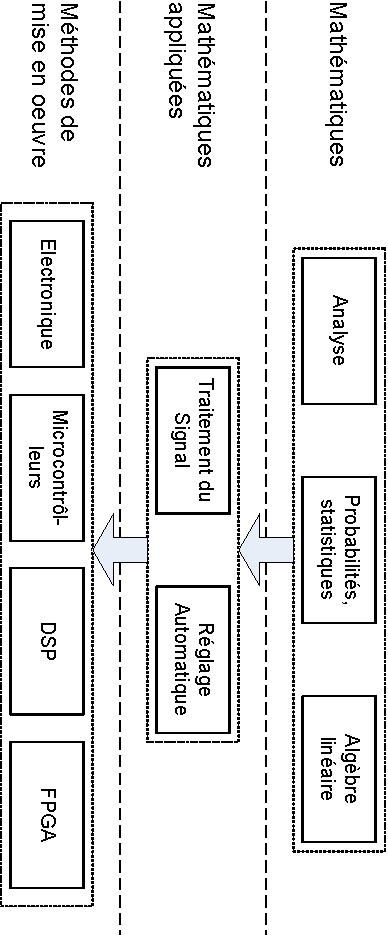
\includegraphics[angle=90, width=14cm]{./Figures/Branches.pdf}
  \rule{35em}{0.5pt}
  \caption[Situation MUI]{Situation du cours MUI dans le cursus de l'ing�nieur}
  \label{fig:Branches}
\end{figure}


\section{D�finitions: processeur, microprocesseur, microcontr�leur et syst�me-on-chip}

Un processeur est un syst�me qui permet l'ex�cution d'op�rations �l�mentaires tel que des op�rations arithm�tiques (additions, soustractions, multiplication et division), des op�rations logiques (OR, AND, XOR), des tests (�gale �, plus petit que, etc.) et des d�placements de donn�es.

Le microprocesseur est un syst�me micro-�lectronique, aussi appel� circuit int�gr� ou plus commun�ment "chip" ou "puce", permettant l'ex�cution d'op�rations �l�mentaires. Contrairement au processeur qui est un concept, le microprocesseur est un composant que l'on place sur un circuit imprim�.

Un microcontr�leur est un syst�me micro-�lectronique contenant un microprocesseur et des p�riph�riques. Les p�riph�riques essentiels sont les minuteries (ou "timers"), les interfaces de communication s�rie et les m�moires (donn�es et instructions).

Le syst�me-on-chip est un ensemble, diff�rent du microcontr�leur, qui inclut tout les composants �lectroniques d'un ordinateur � part les m�moires. Il se pr�sente sous la forme d'un circuit int�gr�. La m�moire de donn�es peut dans certain cas �tre assembl�e en dessus du chip pour r�duire la taille du syst�me.


\section{�l�ments de syst�mes logiques}

Pour pouvoir configurer un microcontr�leur de mani�re efficace, nous avons besoins de quelques �l�ments de syst�mes logiques.

\subsection{D�finitions}
\textbf{Etat logique} : chacune des 2 valeurs que peut prendre une variable logique\\
\textbf{Variable logique} : grandeur qui ne peut prendre que les 2 �tats logiques\\
\textbf{Fonction logique} : variable logique qui d�pend d'autres variables\\
\textbf{Table de v�rit�}: Liste des valeurs de sortie en fonction des combinaisons des entr�es

\begin{table}[!htbp]
\begin{center}
{\fontfamily{phv}\selectfont
\begin{tabular}{|>{\centering}p{.6cm}|c|*{1}{|c}|}
\hline 
\multicolumn{2}{|c|}{Variables} & \multicolumn{1}{|c|}{Sortie}\\
\hline 
A & B & S\\
\hline  
\hline 
0 & 0 & 0\\
\hline 
0 & 1 & 0\\
\hline
1 & 0 & 0\\
\hline
1 & 1 & 1\\
\hline
\end{tabular}
}
\end{center}
\caption{Exemple de table de v�rit� � deux variables \label{table v�rit�}}
\end{table}

La table de v�rit� permet de d�terminer l'�quation logique. Dans l'exemple ci dessus nous avons repr�sent� la fonction $A ET B = S$. Pour construire une table de v�rit� on proc�de de la fa�on suivante: 
\begin{enumerate}
\item on attribue une colonne pour chaque variable ou entr�e (A B C ...)
\item on attribue une colonne pour chaque r�sultat ou sortie
\item on liste toutes les combinaisons des variables d'entr�e ($2^n$ comb.)
\item on calcule le r�sultat pour chaque ligne
\end{enumerate}

\subsection{Fonctions logiques}
Si le nombre de variables d'entr�e n'est pas trop grand, on peut faire l'inventaire exhaustif de toutes les fonctions imaginables:

\begin{table}[!htbp]
\begin{center}
%\begin{tabular}{|p{.5cm}|c||c|c|c|c|c|c|c|c|c|c|c|c|c|c|c|c|}
{\fontfamily{phv}\selectfont
\begin{tabular}{|c|c|*{16}{|c}|}
\hline 
\multicolumn{2}{|c|}{Variables} & \multicolumn{16}{|c|}{Fonctions}\\
\hline 
A & B & F0 & F1 & F2 & F3 & F4 & F5 & F6 & F7 & F8 & F9 & F10 & F11 & F12 & F13 & F14 & F15\\
\hline  
\hline 
0 & 0 & 0 & 0 & 0 & 0 & 0 & 0 & 0 & 0 & 1 & 1 & 1 & 1 & 1 & 1 & 1 & 1\\
\hline 
0 & 1 & 0 & 0 & 0 & 0 & 1 & 1 & 1 & 1 & 0 & 0 & 0 & 0 & 1 & 1 & 1 & 1\\
\hline
1 & 0 & 0 & 0 & 1 & 1 & 0 & 0 & 1 & 1 & 0 & 0 & 1 & 1 & 0 & 0 & 1 & 1\\
\hline
1 & 1 & 0 & 1 & 0 & 1 & 0 & 1 & 0 & 1 & 0 & 1 & 0 & 1 & 0 & 1 & 0 & 1\\
\hline
\end{tabular}
}
$\begin{array}{rclrclcl} \\
F0&=& 0 & \quad F15&=&\overline{F0}&=&1 \\ 
F1&=&A\cdot B & \quad F14&=&\overline{F1}&=&\overline{A \cdot B} \\
F2&=&A \cdot \overline{B} & \quad F13&=&\overline{F2}&=&\overline{A}+B  \\
F3&=&A & \quad F12&=&\overline{F3}&=&\overline{A}  \\
F4&=&\overline{A} \cdot B & \quad F11&=&\overline{F4}&=&A + \overline{B} \\
F5&=&B & \quad F10&=&\overline{F5}&=&\overline{B} \\
F6&=&A \oplus B & \quad F9&=&\overline{F6}&=&\overline{A \oplus B} \\
F7&=&A+B & \quad F8&=&\overline{F7}&=&\overline{A+B} 
\end{array}$
\end{center}

\caption{R�sultats possibles de fonctions � deux variables \label{variable_logiques}}
\end{table}

Dans le tableau pr�c�dent, on peut rep�rer trois fonctions particuli�res :
\begin{enumerate}
\item inversion;
\item fonction dans laquelle une seule configuration des entr�es donne 1;
\item fonction dans laquelle une seule configuration des entr�es donne 0.
\end{enumerate}

\subsection{Op�rateurs �l�mentaires}

Il y a trois fonctions de base qui permettent de cr�er toutes les autres fonctions logiques:
\begin{center}
\begin{tabular}{p{5cm} >{\centering}p{2cm} p{3cm}} 
NON (NOT) &$\overline{A}$ &not A\\
ET (AND) &$A\cdot B$ &A and B\\
OU (OR) &$A+B$ &A or B\\
\end{tabular}
\end{center}
ET et OU sont duals, c-�-d qu'il ont des comportements semblables, mais avec les variables inverses. On peut nommer d'autre fonctions de la table 1.2 par convenance:

\begin{center}
\begin{tabular}{p{5cm} >{\centering}p{2cm} p{3cm}} 
NON ET (NAND) &$\overline{A \cdot B}$ &not(A and B)\\
NON OU (NOR) &$\overline{A+B}$ &not(A or B)\\
OU exclusif (XOR) &$A \oplus B$ &A xor B\\
NON OU exclusif (XNOR) &$\overline{A \oplus B}$ &not(A xor B)\\
\end{tabular}
\end{center}

Ces quatre fonctions suppl�mentaires peuvent toutes s'exprimer en fonction des trois fonctions de base. Pour les fonctions de plus de 2 variables on peut se ramener � une fonction de 2 variables par substitution. Ceci pour montrer que toute fonction logique peut se ramener aux trois fonctions de base.

\subsection{Postulats de l'alg�bre de Boole}
De l'hypoth�se que l'inverse d'une variable ne peut jamais avoir la m�me valeur que la variable, on trouve:
\begin{equation}
\begin{array}{c}
A + \overline{A} = 1 \\
A \cdot \overline{A} = 0
\end{array}
\end{equation}
Ce sont les postulats de l'alg�bre de Boole.

\subsection{Th�or�mes}
Gr�ce aux postulats nous pouvons poser une liste de th�or�mes qui vont nous permettre de simplifier des �quations logiques:

\begin{center}
\begin{tabular}{p{1cm} p{8cm} p{5cm}} 
1&$\overline{\overline{A}}$ &involution not(not A) = A\\
2&$A + 0=A$ &\\
3&$A \cdot 0=0$ &\\
4&$A + 1=1$ &\\
5&$A \cdot 1=A$ &\\
6&$A + A=A$ &idempotence de l'op�rateur OU\\
7&$A \cdot A=A$ &idempotence de l'op�rateur ET\\
8&$A + B = B + A$ &commutativit�\\
9&$A \cdot B=B \cdot A$ &commutativit�\\
10&$A +(B + C) = (A + B)+ C = A+B+C$ &associativit�\\
11&$A \cdot (B \cdot C)= (A \cdot B) \cdot C = A\cdot B\cdot C$ &associativit�\\
12&$A + B \cdot C= (A + B) \cdot (A + C)$ &distributivit�\\
13&$A \cdot (B + C)= (A \cdot B) + (A \cdot C)$ &distributivit�\\
14&$A \cdot B + \overline{A} \cdot B = B$ &absorption\\
15&$\overline{A + B} = \overline{A} \cdot \overline{B}$ &Th�or�me de De Morgan\\
16&$\overline{A \cdot B} = \overline{A} + \overline{B}$ &Th�or�me de De Morgan\\
17&$(A \cdot B) + (\overline{A} \cdot C) + (B \cdot C) = (A \cdot B) + (\overline{A} \cdot C)$ &Th�or�me du Consensus\\
18&$(A + B) \cdot (\overline{A} + C) \cdot (B + C) = (A + B) \cdot (\overline{A} + C)$ &Th�or�me du Consensus\\
\end{tabular}
\end{center}

\subsection{Ecriture canonique}

D�finitions:
\begin{itemize}[label=\textbullet,font=\small]
\item mintermes: les lignes de la table de v�rit� qui donnent 1 comme r�sultat par fonction ET
\item maxtermes: les lignes de la table de v�rit� qui donnent 0 comme r�sultat par fonction OU
\end{itemize}

Par convention, on note $m_{x}$ le minterme tel que x est le nombre d�cimal �gal au code binaire form� par les variables. Par exemple, $m_{5}$ est le minterme correspondant � la configuration [101] des variables d'entr�e.
Par convention, on note $M_{x}$ le maxterme tel que x est le nombre d�cimal �gal au code binaire form� par les variables. Par exemple, $M_{2}$ est le maxterme correspondant � la configuration [10] des variables d'entr�e.
Une cons�quence importante est que les mintermes d�pendent de l'ordre dans lequel les variables sont consid�r�es.

Pour d�terminer la forme canonique d'une fonction logique dont on connait la table de v�rit� on peut faire la somme des mintermes:
\begin{center}
$F = m_1 + m_2 + m_3 + m_6 + m_7$
\end{center}

\begin{center}
\begin{tabular}{*{3}{|c} |c| p{1cm} p{5cm}}
\cline{1-4} 
A & B & C & F\\
\cline{1-4}   
\cline{1-4} 
0 & 0 & 0 & 0\\
\cline{1-4} 
0 & 0 & 1 & 1 & & $\overline{A} \cdot \overline{B} \cdot C = 1$ OU\\
\cline{1-4} 
0 & 1 & 0 & 1 & & $\overline{A} \cdot B \cdot \overline{C} = 1$ OU\\
\cline{1-4} 
0 & 1 & 1 & 1 & & $\overline{A} \cdot B \cdot C = 1$ OU\\
\cline{1-4} 
1 & 0 & 0 & 0\\
\cline{1-4} 
1 & 0 & 1 & 0\\
\cline{1-4} 
1 & 1 & 0 & 1 & & $A \cdot B \cdot \overline{C} = 1$ OU\\
\cline{1-4} 
1 & 1 & 1 & 1 & & $A \cdot B \cdot C = 1$\\
\cline{1-4} 
\end{tabular}
\end{center}

\begin{center}
$F = \overline{A} \cdot \overline{B} \cdot C + \overline{A} \cdot B \cdot \overline{C} + \overline{A} \cdot B \cdot C + 
A \cdot B \cdot \overline{C} + A \cdot B \cdot C$
\end{center}

On peut aussi utiliser l'op�ration duale qui est le produit des maxtermes:
\begin{center}
$F = M_0 \cdot M_4 \cdot M_5$
\end{center}

\begin{center}
\begin{tabular}{*{3}{|c} |c| p{1cm} p{5cm}}
\cline{1-4} 
A & B & C & F\\
\cline{1-4}   
\cline{1-4} 
0 & 0 & 0 & 0 & & $\overline{A} + \overline{B} + \overline{C} = 0$ ET\\
\cline{1-4} 
0 & 0 & 1 & 1\\
\cline{1-4} 
0 & 1 & 0 & 1\\
\cline{1-4} 
0 & 1 & 1 & 1\\
\cline{1-4} 
1 & 0 & 0 & 0 & & $A + \overline{B} + \overline{C} = 0$ ET\\
\cline{1-4} 
1 & 0 & 1 & 0 & & $A + \overline{B} + C = 0$\\
\cline{1-4} 
1 & 1 & 0 & 1\\
\cline{1-4} 
1 & 1 & 1 & 1\\
\cline{1-4} 
\end{tabular}\\
\end{center}

\begin{center}
$F = (\overline{A} + \overline{B} + \overline{C}) \cdot (A + \overline{B} + \overline{C}) \cdot (A + \overline{B} + C)$
\end{center}

Il est ais� de montrer que la somme des mintermes est �gale au produit des maxtermes. Ceci montre encore une fois la dualit� des op�rations logiques. On constate aussi que le nombre de maxtermes est plus petit (3) que celui des mintermes (5). Il est donc plus simple d'utiliser le produit des maxtermes dans ce cas ci.

Le nom mintermes vient du fait que dans une somme de produits, seulement un terme de la somme doit �tre � 1 pour donner un r�sultat de 1. Au contraire, dans un produit de sommes, il faut que toutes les sommes soient � 1 et donc on l'appelle maxtermes.

La forme canonique est rarement optimale, il faut donc la simplifier si on cherche � optimiser l'impl�mentation de la fonction. Il existe des m�thodes manuelles et des m�thodes algorithmiques. On utilisera la m�thode des tables de Karnaugh pour une r�duction manuelle si le nombre de variables est limit�. Au del� de 4 variables on a int�r�t � utiliser une m�thode algorithmique tel que celle de Quine-McCluskey.

\subsection{Op�rateurs logiques en C}

La programmation des microcontr�leurs s'effectue principalement en C (2016). Nous avons donc besoin de savoir comment les op�rations logiques sont repr�sent�es dans ce langage. En C, on diff�rentie la logique sur 1 bit appel�e "bit � bit" de celle sur un mot complet (8-16-32 bits). En effet, les deux types produisent des r�sultats diff�rents car le FAUX sur un mot est bien '00000000' par exemple mais le VRAI comprend toutes les autres valeurs.


\begin{table}[!htbp]
\begin{center}
\begin{tabular}{|c|c|c|c|}
\hline
Op�rateur & Signification & Notation C & Utilisation typique\\
\hline
AND & ET & \& & For�age � 0 d'un bit dans un registre\\
OR & OU & | & For�age � 1 d'un bit dans un registre\\
XOR & OU exclusif & \^{} & Inversion d'un bit dans un registre\\
NOT & inversion & $\sim$ & Inversion de tous les bits d'un registre\\
\hline
\end{tabular}
\end{center}
\caption{Op�rateurs logiques bit � bit en C}
\end{table}

Exemple: 
\lstset{style=customc}
\begin{lstlisting}
char REG;
REG &= 0x7F; //force � 0 le bit no 7
\end{lstlisting}

\begin{table}[!htbp]
\begin{center}
\begin{tabular}{|c|c|c|c|}
\hline
Op�rateur & Signification & Notation C & Utilisation typique\\
\hline
AND & ET & \&\& & Test logique\\
OR & OU & || & Test logique\\
NOT & n�gation & ! & Test logique\\
 & �quivalence & == & Test logique\\
\hline
\end{tabular}
\end{center}
\caption{Op�rateurs logiques bool�ens en C}
\end{table}

Exemple: 
\lstset{style=customc}
\begin{lstlisting}
if (REG == 0x0F)
	printf("REG est �gal � 0x0F\n");
\end{lstlisting}

Les op�rateurs bit � bit s'utilisent souvent pour la configuration de registres dans les microcontr�leurs, exemple:

\lstset{style=customc}
\begin{lstlisting}
REG = P1IN & (BIT5 | BIT2);
\end{lstlisting}

Les op�rateurs bool�ens quand � eux s'utilisent surtout dans la simplification d'expressions, exemple:

\lstset{style=customc}
\begin{lstlisting}
if (!(!x && !y)) est �quivalent � if (x || y)
\end{lstlisting}

%\begin{thebibliography}{1}
%
%\bibitem[1]{decoulon}Fr�d�ric de Coulon, \emph{Th�orie et traitement des signaux}, Presses polytechniques romandes, 1990
%
%\bibitem[2]{proakis}John G. Proakis, Dimitris G. Manolakis: \emph{Digital Signal Processing}, Pearson Prentice Hall, 2007
%
%\end{thebibliography}
 

\chapter{\textsc{GPIO (General Purpose Input Output)}}

Le GPIO (General Purpose Input/Output) est une broche d'entr�e ou sortie � usage g�n�rique. Les GPIOs sont group�es en ports de 8bits ou 16bits. Au sein d'un port ont peut acc�der � chaque broche ind�pendamment en utilisant un masque (voir �2.2).

Les GPIOs sont configur�s � l'aide de registres qui ont la dimension d'un port (8 ou 16 bits). Un port est donc juste un groupe de GPIOs qui permet une �criture simplifi�e du code.


\section{Mat�riel}

Les GPIOs sont pr�sents sur tout les microcontr�leurs en nombre plus ou moins grande d�pendamment du nombre de broche disponible sur le bo�tier. On choisit souvent un microcontr�leur en fonction du nombre de GPIO disponibles.

Le fonctionnement mat�riel du GPIO est d�crit � la fig. \ref{fig:gpio}. 

\begin{figure}[htb]
  \centering
  \includegraphics[angle=90, trim = 25mm 0mm 15mm 0mm, clip, width=14cm]{./Figures/gpio/port.pdf}
  \rule{35em}{0.5pt}
  \caption[port GPIO]{Description mat�riel d'un GPIO}
  \label{fig:gpio}
\end{figure}

Il contient trois parties principales:
\begin{itemize}[label=\textbullet,font=\small]
\item Le circuit de sortie
\item Le circuit d'entr�e
\item Un ou plusieurs commutateurs pour connecter la broche
\end{itemize}

Au del� du circuit de base d�crit auparavant, il existe d'autres fonctions optionnelles dans les GPIO comme une synchronisation ou un circuit pour traiter des interruptions (voir ch. 4)

\subsection{Input}

Dans la partie "entr�e" du GPIO on trouve un tampon qui m�morise la valeur logique pr�sente � l'entr�e ainsi qu'un bloc pour s�lectionner une r�sistance de pull-up ou pull-down. Ce bloc est tr�s important car il est n�cessaire pour �viter qu'une entr�e se retrouve flottante. Si une entr�e est laiss�e non-connect�e (flottante) elle peut alors prendre n'importe quel valeur et m�me changer de valeur al�atoirement au cours du temps. Pour �viter se ph�nom�ne on doit utilise une r�sistance plac�e selon le sch�ma suivant fig. \ref{fig:pullres}.

\begin{figure}[htb]
  \centering
  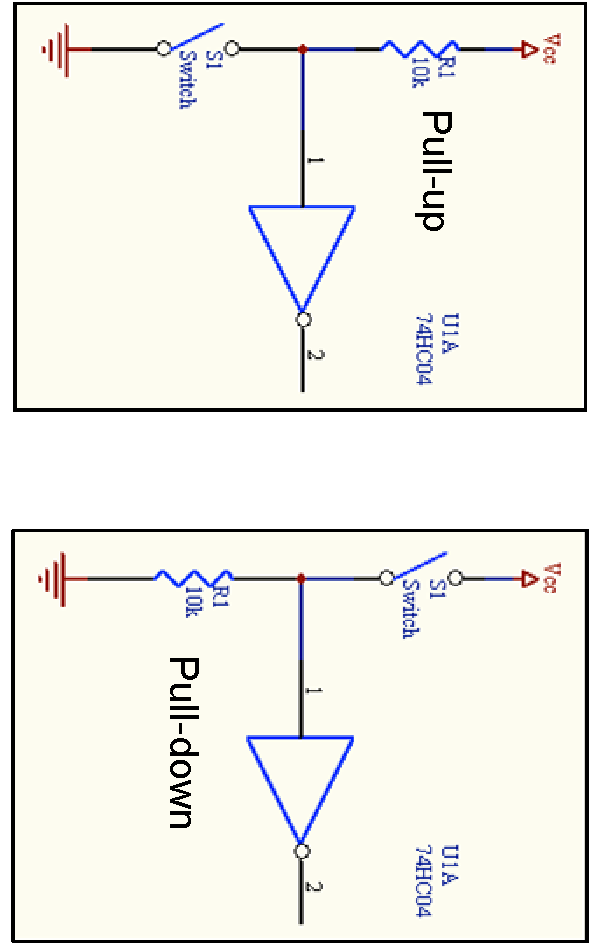
\includegraphics[angle=90, width=10cm]{./Figures/gpio/pullres.pdf}
  \rule{35em}{0.5pt}
  \caption[res pull]{R�sistances de pull-up et pull-down}
  \label{fig:pullres}
\end{figure}

La valeur de cette r�sistance est choisie de mani�re optimale entre deux facteurs: i) le courant consomm� VCC-GND qui doit �tre le plus faible possible quand l'interrupteur est ferm� et ii) La vitesse � laquelle la r�sistance d�charge la capacit� d'entr�e du circuit int�gr� CMOS lorsque l'interrupteur est ouvert. Les valeurs typiques se situent entre $10k\Omega$ et $100k\Omega$. Mais attention sous 3.3V, �a consommera lorsque l'interrupteur est ferm�, entre $330�A$ et $33�A$ ce qui n'est pas n�gligeable!

Dans le cas particulier du MSP430F5529 la valeur typique des r�sistances de pull est de $35k\Omega$ ce qui provoque un courant de $86\mu A$ sous 3V. Il est donc avantageux de choisir un interrupteur poussoir plut�t que commutant pour minimiser le temps total de consommation. On peut aussi r�duire la tension d'alimentation � 1.8V pour r�duire le courant mais attention � la r�duction de vitesse du microcontr�leur.

\subsection{Output}

Dans la partie "sortie" du GPIO on trouve un tampon qui m�morise la valeur logique que l'on veut sortir sur la broche ainsi qu'un amplificateur pour permettre au circuit de commuter la charge de sortie rapidement. Cette charge est souvent de type capacitive avec une valeur comprise entre 2pF et 10pF typiquement. On peut donc calculer le courant n�cessaire pour charger cette capacit� � 90\% dans un temps voulu. Ensuite on peut ajuster le courant, si disponible dans le GPIO, pour atteindre la vitesse recherch�e.

\section{Logiciel}

Pour programmer les GPIOs on utilise des registres organis�s en ports. Par exemple dans la nomenclature Texas Instrument [], le port1 contient huit GPIO et on les nommes P1.0 � P1.7. On peut aussi utiliser le groupement par seize o� la notation devient PA, PB, etc. PA est �quivalent aux ports P0 et P1 regroup�s alors que PB est �quivalent aux ports P2 et P3. 

\subsection{Programmation par masque}

Comme les GPIO sont group�s en paquets de 8 ou 16 du point de vue logiciel, il faut un moyen pour programmer chaque GPIO individuellement. Cela signifie que si on modifie un GPIO, il ne faut surtout pas affecter les autres du m�me groupe. Un moyen d'arriver � ceci est d'utiliser un masque qui repr�sente le bit d�sir�. Par exemple si on d�sire s�lectionner le bit 3 on utilisera le masque BIT3 = 00001000 sur 8 bits (La num�rotation commence � z�ro). Si on d�sire s�lectionner le bit 3 sur 16 bits alors le masque sera BIT3 = 0000000000001000.

Soit un registre (REG) de 8 bits servant � configurer 8 broches d'un microcontr�leur (fig \ref{fig:pxout}). 

\begin{figure}[htb]
  \centering
  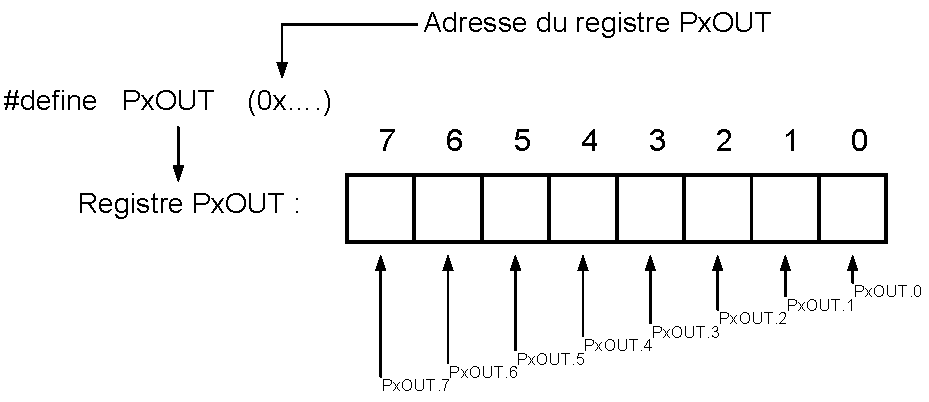
\includegraphics[angle=0, width=10cm]{./Figures/gpio/PxOUT.pdf}
  \rule{35em}{0.5pt}
  \caption[buff out]{Tampon de sortie}
  \label{fig:pxout}
\end{figure}

Pour mettre � 1 le bit 0 sans changer les bits 1 � 7 on peut utiliser la fonction OU, REG = REG OU BIT0 avec BIT0 = 00000001:

\lstset{style=customc}
\begin{lstlisting}
REG = REG | BIT0  //en C avec BIT0 = 1
REG |= BIT0		  //en C simplifi�
\end{lstlisting}

On appelle cette technique le masquage. Pour mettre un bit � 0, il faut utiliser une autre fonction logique car le OU logique ne fait rien avec un z�ro. Il est int�ressant de r�soudre ce probl�me par soi-m�me pour trouver la solution. On cherche donc � mettre un bit � 0 sans changer l'�tat logique des autres bits du port. Pour trouver la solution on peut partir d'un exemple et proc�der par �limination:

\lstset{style=customc}
\begin{lstlisting}
REG = 00000011    //on d�sire mettre le premier bit � z�ro sans influencer les autres
\\test avec OU:
REG = REG | BIT0  //ne fait rien donc ce n'est pas la solution
\\test avec ET:
REG = REG & BITO  //REG = 00000001 FAUX �a ne marche pas non plus
\end{lstlisting}

Mais si on avait invers� BIT0 alors �a aurait march�:

\lstset{style=customc}
\begin{lstlisting}
REG = REG & ~BITO   //REG = 00000010 JUSTE 
REG ~& BIT0         //en C simplifi�
\end{lstlisting}

On constate donc qu'il faut utiliser la fonction duale mais avec une inversion pr�alable. Ceci convient pour l'�criture dans un registre mais quand est-il de la lecture? Comment pourrait-on lire un GPIO parmi tous les bits d'un port?

La r�ponse est similaire au test d'un bit dans un mot en langage C. Prenons comme exemple la lecture, ou test, du BIT0 dans REG et proc�dons par �limination. Il faut trouver la fonction d�sir�e avec par exemple REG = 00000011 et BIT0 = 00000001:

\lstset{style=customc}
\begin{lstlisting}
//essai avec OU avec REG = 00000011 et BIT0 = 00000001:
TEST_BIT0 = REG | BIT0  //TEST_BIT0 = 00000011 FAUX
//et si REG = 00000010
TEST_BIT0 = REG | BIT0  //TEST_BIT0 = 00000011 FAUX

//Il est clair que �a ne marche pas avec OU essayons avec ET:
TEST_BIT0 = REG & BIT0  //TEST_BIT0 = 00000001 JUSTE
//et si REG = 00000010
TEST_BIT0 = REG & BIT0  //TEST_BIT0 = 00000000 JUSTE
\end{lstlisting}

Donc le test ou lecture d'une valeur s'effectue avec l'op�rateur logique ET. Dans le cas d'un test en C, on doit se rappeler que le r�sultat est VRAI pour toute valeur de TEST\_BITx diff�rente de z�ro. Il est faux si et seulement si TEST\_BITx = 0. Ceci provient du fait que la variable C la plus petite est de 8 bits. Il n'y a pas de variable de 1 bit en C. 

\subsection{�criture dans un registre}

Soit le registre REG d'une longueur de 8 bits. Pour �crire la valeur logique 1 dans le registre on utilise la fonction OU entre le registre et le masque du bit voulu. Pour �crire un 0 logique on utilise la fonction ET entre le registre et le masque du bit voulu invers�, exemples:

\lstset{style=customc}
\begin{lstlisting}
//Mise � 1 du bit z�ro:
REG = REG | BIT0    //en C avec BIT0 = 1
REG |= BIT0		    //en C simplifi�

//Mise � 0 du bit z�ro:
REG = REG & ~BITO   //REG = 00000010 JUSTE 
REG ~& BIT0         //en C simplifi�
\end{lstlisting}

Pour la mise � 1 ou 0 simultan�e de plusieurs bits on utilise le OU pour sommer les masques et cr�er un masque contenant les deux bits. Exemple: BIT3 | BIT0 = 00001001:

\lstset{style=customc}
\begin{lstlisting}
//Mise � 1 du bit z�ro et trois simultan�ment:
REG |= BIT0 | BIT3

//Mise � 0 du bit z�ro et trois simultan�ment:
REG ~& BIT0 | BIT3
\end{lstlisting}

\subsection{Lecture d'un registre}

Pour lire un registre on compare le registre avec le masque du bit voulu en utilisant la fonction ET: 

\lstset{style=customc}
\begin{lstlisting}
//Lecture du BIT3 uniquement:
TEST_REG = REG & BIT3; // BIT3=00001000
\end{lstlisting}

Le r�sultat de cette affectation sera donc 0 si le BIT3 est � z�ro et 8 si le BIT3 est � 1. Pour lire plusieurs bits � la fois on peut, comme pour l'�criture, cr�er un masque combin�. Exemple, on veut lire le bit 5 et le bit 2 simultan�ment:

\lstset{style=customc}
\begin{lstlisting}
//Lecture du BIT5 et du BIT2:
TEST_REG = REG & (BIT5 | BIT2); // BIT5 | BIT2 = 00100100
\end{lstlisting}

\section{Configuration des GPIO}

Avant de pouvoir utiliser un GPIO il faut le configurer. Cela inclus principalement:

\begin{itemize}[label=\textbullet,font=\small]
\item Le multiplexeur d'entr�e
\item La fonction entr�e ou sortie
\item La r�sistance de pull-up ou pull-down lorsqu'on est en entr�e
\end{itemize}

Pour les configurer on doit trouver leurs adresses physiques qui les identifient � l'int�rieur du circuit int�gr�. Ces adresses peuvent �tre trouv�es dans la documentation du microcontr�leur mais souvent elle sont fournie sous forme de constantes dans une librairie qu'on peut inclure dans le code C.

\lstset{style=customc}
\begin{lstlisting}
#include <msp430.h>

#define P1IN   	(PAIN_L)       /* Port 1 Input */
#define P1OUT 	(PAOUT_L)      /* Port 1 Output */
#define P1DIR	(PADIR_L)      /* Port 1 Direction */
#define P1REN	(PAREN_L)      /* Port 1 Resistor Enable */
#define P1DS 	(PADS_L)       /* Port 1 Drive Strength */
#define P1SEL	(PASEL_L)      /* Port 1 Selection */
\end{lstlisting}

Exemple de configuration du port P1.2 et P1.5 en sortie:

\lstset{style=customc}
\begin{lstlisting}
P1SEL &= ~BIT5 & ~BIT2;  // Reset P1.2 et P1.5 to select GPIO
P1DIR |=  BIT5 | BIT2;   // Set P1.2 et P1.5 to output direction
//Option: ajouter le P1DS pour changer le courant de sortie

//Puis �criture sur les sorties P1.5 et P1.2 d'un 1 logique:
P1OUT |= BIT5 | BIT2;
\end{lstlisting}

Exemple de configuration du port P1.2 et P1.5 en entr�e:

\lstset{style=customc}
\begin{lstlisting}
P1SEL &= ~BIT5 & ~BIT2;  // Reset P1.2 et P1.5 to select GPIO
P1DIR &= ~BIT5 & ~BIT2;  // Reset P1.2 et P1.5 to input direction
//Option: ajouter les r�sistances de pull
P1OUT |= BIT5 | BIT2;    // S�lection de la r�sistance
P1REN |= BIT5 | BIT2;    // Activation de la r�sistance

//Puis lecture de l'entr�e P1.5 et P1.2:
TEST_REG = P1IN & (BIT5 | BIT2);
\end{lstlisting}

 

\chapter{\textsc{Numération et arithmétique des ordinateurs}}
La représentation des nombres, ainsi que l'arithmétique, est très critique pour une utilisation optimale par un processeur. Historiquement on a cherché des méthodes qui minimisent le nombre d'opérations à effectuer pour réduire la taille du matériel. Bien qu'aujourd'hui ce ne soit plus si critique, c'est toujours important pour maximiser la vitesse et minimiser la consommation des processeurs.

\section{Codage binaire et hexadécimal}
Il est utile de rappeler le codage des nombres entiers positifs en base 2 et 16 avant de progresser vers les nombres négatifs et les nombres fractionnaires:

\begin{table}[!htbp]
\begin{center}
{\fontfamily{phv}\selectfont
\begin{tabular}{|c|c|c||c|c|c|}
\hline 
Entier & Binaire & Hexadécimal & Entier & Binaire & Hexadécimal\\
\hline  
0 & 0000 & 0 & 8 & 1000 & 8\\
1 & 0001 & 1 & 9 & 1001 & 9\\
2 & 0010 & 2 & 10 & 1010 & A\\
3 & 0011 & 3 & 11 & 1011 & B\\
4 & 0100 & 4 & 12 & 1100 & C\\
5 & 0101 & 5 & 13 & 1101 & D\\
6 & 0110 & 6 & 14 & 1110 & E\\
7 & 0111 & 7 & 15 & 1111 & F\\
\hline 
\end{tabular}
}
\end{center}
\caption{Codage binaire et hexadécimal des entiers positifs sur 4 bits \label{binaire hexa}}
\end{table}

%\newpage 
\section{Représentation des nombres}
Les circuits logiques, composants des processeurs, ne fonctionnent qu'en binaire. Il faut donc convertir tous les nombres usuels, pour pouvoir les utiliser. Il est aisé d'attribuer un code binaire à un nombre donné. Par exemple 000 pour le zéro et 001 pour le 1. Mais ceci devient un problème lorsqu'on ajoute le signe moins et la virgule qui ne sont pas des chiffres.

\subsection{Entiers} 
On représente les entiers positifs simplement à l'aide d'une conversion décimale-binaire directe (Table \ref{binaire hexa}).

Pour les nombres entiers négatifs nous devons faire un choix, prenons par exemple le codage avec 4 bits. Nous avons donc $2^4 = 16$ codes différents disponibles et nous devons aussi coder le zéro ce qui donne $16 - 1$ nombres disponibles. Comme c'est impaire nous aurons soit un nombre de plus du coté positif ou un nombre de plus du coté négatif. Le choix fait a été celui d'avoir un nombre négatif de plus (Table \ref{entiers négatifs}). Ce qui donne $2^{n-1}$ du côté positif pour accommoder le zéro et $2^n$ du côté négatif.

\paragraph{Complément à deux}
Il nous reste à déterminer quels codes attribuer aux nombres négatifs. En effet on peut choisir de placer les nombres négatifs à la suite des nombres positifs \textbf{ou} avant le zéro en faisant le calcul $0-1$ en binaire ou encore en décalant tous les nombres. Comparons les trois possibilités et notons bien les différences:

\begin{table}[!htbp]
\begin{center}
{\fontfamily{phv}\selectfont
\begin{tabular}{|c|c|c|c|}
\hline 
Entier & Cas 1 & Cas 2 & Cas 3\\
\hline  
\hline 
0 & 0000 & 0000 & 1000\\
\hline 
1 & 0001 & 0001 & 1001\\
\hline
7 & 0111 & 0111 & 1111\\
\hline
-1 & 1000 & 1111 & 0111\\
\hline
-2 & 1001 & 1110 & 0110\\
\hline
-8 & 1111 & 1000 & 0000\\
\hline
\end{tabular}
}
\end{center}
\caption{Trois possibilités pour coder les nombres entiers négatifs \label{entiers négatifs}}
\end{table}

On constate que le cas 1 offre une discontinuité entre -1 et 0 ce qui rend cette notation peu intéressante d'un point de vue arithmétique. Ce n'est donc pas utilisé en pratique.

Les cas 2 et 3, par contre, sont symétriques par rapport à zéro ce qui permet de faire l'opération $0-1$ sans erreur. Tous les nombres sont continus ce qui est souhaitable.

Le cas 3 à la particularité d'avoir le zéro décimal à un nombre différent du zéro binaire mais ce n'est pas un problème en soit. Ce cas est souvent utilisé pour coder l'exposant des nombres en virgule flottante et s'appelle \textbf{décalage par excès}. L'excès étant la valeur de décalage de l'échelle qui correspond au zéro décimal, e.g. 1000 = 8 (excès).

Dans le cas 2 on peut remarquer aussi que le nombre de gauche vaut "0" pour un nombre positif et "1" pour un nombre négatif, c'est pour cela qu'on l'appelle aussi bit de signe. Noter bien que si on avait choisi de coder les nombres de -7 à 8, à la place de -8 à 7, le bit de signe ne serait pas possible. Ceci est du au fait que le zéro n'a pas de signe. En pratique et en grande majorité, on préfère ce dernier et on le nomme \textbf{complément à deux}. 

Le nom \textbf{complément à deux} est une contraction de complément modulo 2. Un nombre binaire en complément à deux se calcule donc par le complément à $2^n$ du nombre non signé:
\begin{equation}
A_{comp2} = 2^n - |A|
\end{equation}
On part donc du chiffre le plus élevé et on décrémente. Exemple pour A = -1 sur 4 bits, $A_{comp2} = 2^4 - 1 = 15 = 1111$.

Le grand mérite de la notation en complément à deux est le fait qu'on peut additionner sans se préoccuper du signe alors que si on avait choisi une autre notation il aurait fallu utiliser une condition sur le signe pour en tenir compte. Pour vérifier prenons deux nombres m et r sur n bits et effectuons tous les cas de signe:

\begin{equation}
\begin{aligned}
+m \equiv m \enspace & \enspace +r \equiv r\\
-m \equiv 2^n-m \enspace & \enspace -r \equiv 2^n-r\\
(+m) + (+r) \enspace &= \enspace m + r\\
(-m) + (+r) \enspace &= \enspace 2^{n} - m + r = r-m\\
(+m) + (-r) \enspace &= \enspace m + 2^{n} - r = m-r\\
(-m) + (-r) \enspace &= \enspace 2^{n} - m + 2^{n} - r = -m-r
\end{aligned}
\end{equation}
Les $2^n$ n'affectent pas les résultats par arithmétique modulo $2^n$. On constate donc que tous les résultats sont corrects quelque soit le signe. 

\paragraph{Négation d'un nombre positif}
De la Table \ref{entiers négatifs}, on peut constater qu'il suffit d'inverser les bits du nombre positif puis d'y ajouter "1" pour obtenir la négation:

\begin{equation}
-A = \overline{A} - 1
\end{equation}

C'est une manière plus rapide de calculer le complément modulo 2. Une démonstration algébrique est donnée en annexe.
 
\paragraph{Extension d'un nombre entier}
Dans le cas ou on désire passer d'un format de n bits à m bits avec m supérieur à n, on doit remplir les cases vides m-n. Il est trivial que les cases vides d'un nombre positif doivent être des zéros, exemple, 1 sur 4 bits: 0001 et sur 8 bits: 00000001. L'extension des nombres positifs consiste donc à ajouter autant de zéros que nécessaire, mais quand est-il des nombres négatifs en complément à 2? Prenons un exemple -1 qui est 1111 sur 4 bits et si on ajoute des zéros cela donne 00001111 = 8 en complément à deux, ça ne marche pas. Pour qu'un nombre négatif reste négatif, il faut que son bit de signe soit "1", on devrait donc mettre 10001111 = -112 ce qui ne joue toujours pas. On peut trouver la réponse en faisant l'opération 0 - 1 sur 8 bits et on trouve 11111111 = -1. On constate donc que pour les nombres négatifs, il faut ajouter des "1" dans les case vides. Une démonstration algébrique vous est proposée en annexe.
 
%\newpage
\subsection{Virgule flottante}
Pour les nombre réels, on doit coder la virgule et sa position en plus du signe. Ceci complique la représentation car il faut un deuxième nombre, qui est un entier, pour représenter la position de la virgule. On choisit de préférence d'utiliser  ce nombre pour représenter un exposant plutôt qu'une position de virgule mais ça reviens au même.

\begin{equation}
X dans \, \mathbb{R} = signe \cdot m \cdot 2^{exposant}
\end{equation}

Exemple de codage avec 8 bits:
\begin{center}
{\fontfamily{phv}\selectfont
\begin{tabular}{|c|c|c|c|c|c|c|c|}
\hline
signe & m3 & m2 & m1 & m0 & e2 & e1 & e0 \\
\hline
\end{tabular}
}
\end{center}

Noter bien que l'exposant peut être positif ou négatif d'où la nécessité de choisir un format pour l'exposant comme le complément à deux ou le décalage par excès (le décalage consiste simplement à soustraire $2^{n-1}$ pour retrouver une moitié négative).

%\newpage 
\subsection{Virgule fixe}
On peut simplifier la représentation des nombre réels si la virgule est fixe, c-à-d si l'exposant ne change pas. Ceci est très utilisé dans les processeurs qui ne possèdent pas d'unité de calcul en virgule flottante.

\begin{center}
{\fontfamily{phv}\selectfont
\begin{tabular}{|c|c|c|c c|c|c|c|}
\hline
0 & 0 & 0 & 1 . & 0 & 0 & 0 & 0 \\
\hline
\end{tabular}
}
\end{center}

Dans l'exemple ci-dessus nous avons 4 bits pour le nombre entier et 4 bits pour le nombre fractionnaire. La virgule n'est pas codée en tant que tel et le nombre complet utilise 8 bits. Seul deux constantes sont nécessaires pour décrire le format en virgule fixe: la longueur de la partie entière et la longueur de la partie fractionnaire:

\lstset{style=customc}
\begin{lstlisting}
#define FIXEDPT_IBITS	4
#define FIXEDPT_FBITS	4
\end{lstlisting}

\section{Opérateurs}
Les opérations arithmétiques sont différentes pour chaque format de nombre mais elles peuvent toutes se ramener à un additionneur 1 bit qui se réalise facilement à l'aide d'un porte logique XOR et AND. 

\begin{table}[!htbp]
\begin{center}
{\fontfamily{phv}\selectfont
\begin{tabular}{|c|c|c|c|}
\hline 
A & B & A + B & Retenue\\
\hline  
\hline 
0 & 0 & 0 & 0\\
\hline 
0 & 1 & 1 & 0\\
\hline
1 & 0 & 1 & 0\\
\hline
1 & 1 & 0 & 1\\
\hline
\end{tabular}
}
\end{center}
\caption{Table de vérité de l'additionneur 1 bit \label{add 1 bit}}
\end{table}

\begin{figure}[htb]
  \centering
  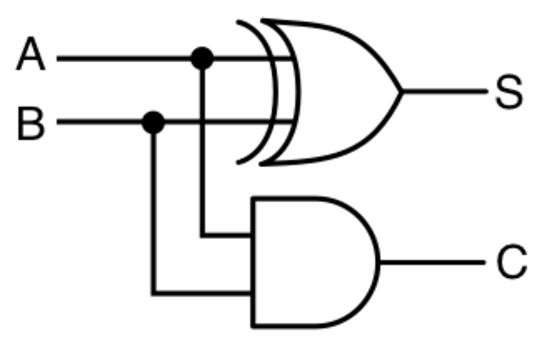
\includegraphics[width=5cm]{./Figures/arith/Half-adder.pdf}
  \rule{35em}{0.5pt}
  \caption[half_adder]{Réalisation de l'additionneur 1 bit (sans entrée de retenue)}
  \label{fig:half_adder}
\end{figure}

Le circuit complet d'un additionneur 1 bit doit encore sommer une retenue éventuelle en entrée donc en réalité il additionne 3 bits. Exactement de la même manière que lorsqu'on calcule en colonnes à la main.

\subsection{Addition}
Additionner deux nombres entiers positifs est évident mais attention aux débordements! Par exemple: 4 + 4 = 8, sur 4 bits (n=4) en complément à deux, nous n'avons pas de code pour le 8. Pour comprendre ce qu'il se passe, effectuons l'addition en binaire:

\begin{center}
{\fontfamily{phv}\selectfont
\begin{tabular}{c c c}
  & 0100 & 4 \\
+ & 0100 & 4 \\
\hline
  & 1000 & -8 \\
\end{tabular}
}
\end{center}

Selon ce calcul, nous avons donc un résultat de -8 à la place de +8. Il faut donc un mécanisme pour nous avertir quand un débordement se produit (voir chapitre 8).

Nous avons un problème similaire lors de l'addition de deux nombres entiers négatifs, par exemple: -4 + (-5) = -9. Si nous faisons le calcul en représentation en complément à deux sur 4 bits:

\begin{center}
{\fontfamily{phv}\selectfont
\begin{tabular}{c c c}
  & 1100 & -4 \\
+ & 1011 & -5 \\
\hline
  & 0111 & +7 \\
\end{tabular}
}
\end{center}

On peut constater que le débordement conduit à retourner au nombre le plus élevé de l'autre côté de la gamme. En binaire, le calcul s'effectue, débordement ou pas, et le processeur continue comme si de rien n'était. On appelle ceci, l'arithmétique modulo $2^n$. L'opération modulo, par exemple en langage C, retourne le reste de la division entière d'un nombre. Cette opération s'effectue automatiquement à l'aide d'une addition en arithmétique modulo, par exemple en représentation 4 bits non-signée: (8 + 9) modulo 16 = 1. Pour bien comprendre effectuons l'addition en binaire:
 
\begin{center}
{\fontfamily{phv}\selectfont
\begin{tabular}{c c c}
  & 1000 & 8 \\
+ & 1001 & 9 \\
\hline
  & 0001 & 1 \\
\end{tabular}
}
\end{center}

Le résultat de l'addition est bien celui du reste de la division entière par 16.

L'addition en virgule fixe reste la même que l'addition pour les entiers mais l'addition en virgule flottante est très différente car il faut ajuster l'exposant.

\subsection{Soustraction}
La soustraction peut se décomposer en un changement de signe et une addition ce qui permet de se ramener aux cas ci-dessus. 

\begin{equation}
A - B = A + (-B)
\end{equation}

De plus un seul composant matériel, l'additionneur, est nécessaire pour les deux opérations. La négation ne nécessite qu'une inversion et l'ajout de "1" qui s'effectue aussi à l'aide du même additionneur.

\subsection{Multiplication}
On peut décomposer une multiplication en sommes de produits qui se ramène d'un point de vue matériel à des additions et des décalages. Prenons un exemple 3 x 5 sur 4 bits (n=4) non signé:

\begin{center}
{\fontfamily{phv}\selectfont
\begin{tabular}{c r r}
  & 0011 & 3 \\
x & 0101 & 5 \\
\hline
& 00000011 \\
& 00000000 \\
& 00001100 \\
& 00000000 \\
\hline
& 00001111 & 15 \\
\end{tabular}
}
\end{center}

On constate donc qu'il suffit de créer quatre produits intermédiaires qui sont juste des décalages du nombre 3 lorsque le nombre multipliant est non nul. Ensuite on fait la somme des quatre nombres avec un additionneur. Noter bien que si on décale de 4 crans vers la gauche, le nombre intermédiaire à une taille de 8 bits. Les résultats sont donc sur $2n$ bits.

Le cas des nombres négatifs est différent au niveau de l'extension des nombres intermédiaires. En effet, dans notre multiplication ci-dessus nous avons introduit des zéros pour étendre un nombre. Prenons l'exemple suivant (-3) x 2 sur 4 bits signés:

\begin{center}
{\fontfamily{phv}\selectfont
\begin{tabular}{c r r}
  & 1101 & -3 \\
x & 0010 & 2 \\
\hline
& 00000000 \\
& 11111010 \\
& 00000000 \\
& 00000000 \\
\hline
& 11111010 & -6\\
\end{tabular}
}
\end{center}

Dans ce cas ci, nous devons étendre le nombre intermédiaire négatif avec des "1" pour obtenir la bonne solution. Le résultat reste -6 quelque soit le nombre de "1" devant le nombre (1010 = -6, 11111010 = -6). Le changement des bits de l'extension nécessite une condition sur le signe qui rend le calcul d'un nombre signé plus long que celui d'un nombre non-signé. Il faut donc une autre technique pour un processeur qui est indépendante du signe.

La multiplication de nombres en virgule fixe est légèrement différente car il faut décaler le résultat de multiplication de la taille de la partie fractionnaire vers la droite:

\lstset{style=customc}
\begin{lstlisting}
#define FIXEDPT_IBITS	8
#define FIXEDPT_FBITS	8

typedef int16_t fixedpt;

/* Multiplies two fixedpt numbers, returns the result. */
fixedpt fixedpt_mul(fixedpt A, fixedpt B)
{
	return (((fixedptd)A * (fixedptd)B) >> FIXEDPT_FBITS);
}
\end{lstlisting}

Le but de ce décalage est de replacer la virgule au bon endroit dans le résultat car le nombre de bits de la partie fractionnaire vaut $2n$ et donc il faut le décaler de $n$ à droite.

\paragraph{Réduction de la complexité du calcul de la multiplication}
En faisant le calcul selon la méthode en colonnes trois problèmes se posent:
\begin{enumerate}
\item Le nombre de produits intermédiaires est de $n$ ce qui nécessite $n$ emplacements de mémoire sous forme de registres rapides pour effectuer le calcul à la vitesse maximum. 
\item La taille des résultats intermédiaires vaut $2n$ donc il faut des emplacements mémoire doubles.
\item Si une des opérandes est négative alors il faut calculer sans le signe puis effectuer une correction
\end{enumerate}
Le premier problème peut se résoudre en accumulant le résultat intermédiaire au fur et à mesure. Le deuxième en ne mémorisant que les n bits de poids fort. Le dernier problème en utilisant l'\textbf{algorithme de Booth} (voir annexe \ref{ch:algebra}). 

\subsection{Division}
La division entière ou Euclidienne est très simple à implémenter à l'aide de la soustraction successive du diviseur:

\lstset{style=customc}
\begin{lstlisting}
int divide(N, D) {
	Q = 0;
	while  N >= D {
  		N = N - D;
  		Q++;
	}
	return Q;			//ou N pour le reste
}
\end{lstlisting}

La division entière peut donc s'effectuer avec un additionneur, une négation et un test. Le temps d'exécution est par contre relativement long si N>>D.

Pour le cas de la virgule fixe, il faut décaler le multiplicande vers la gauche avant division:

\lstset{style=customc}
\begin{lstlisting}
#define FIXEDPT_IBITS	8
#define FIXEDPT_FBITS	8

typedef int16_t fixedpt;

/* Divides two fixedpt numbers, returns the result. */
static inline fixedpt
fixedpt_div(fixedpt A, fixedpt B)
{
	return (((fixedptd)A << FIXEDPT_FBITS) / (fixedptd)B);
}
\end{lstlisting}

Comme pour la multiplication, il existe des algorithmes plus efficaces pour faire la division entière comme celui appelé SRT.

\section{Exercices}

\paragraph{Ex 1}
Implémenter l'algorithme de Booth en C puis en assembleur.

\paragraph{Ex 2}
Écrire en C une fonction de division de deux nombres entiers en complément à 2 qui retourne le résultat en utilisant seulement des additions ou des soustractions. Attention aux signes et à la division par zéro.

\paragraph{Ex 3}
Implémenter l'algorithme SRT en C.


     

\chapter{\textsc{Interruptions}}

Les interruptions sont une m�thode pour g�rer l'ex�cution de t�ches simultan�es. Elles se ram�nent � la notion de parall�lisme dans les processeurs d'ordinateurs. La probl�matique provient du fait qu'un processeur ex�cute une t�che � la fois et qu'il est fr�quent que plusieurs �v�nements apparaissent simultan�ment comme par exemple lorsqu'on appuie sur une touche et que le processeur effectue un calcul. 

\section{Interaction entre le processeur et les p�riph�riques}
Le processeur ex�cute des programmes et en m�me temps il interagit avec les p�riph�riques. Il existe deux possibilit�s pour effectuer toutes les t�ches, le sondage et les interruptions.

\subsection{Sondage}
Le sondage consiste � lire l'�tat d'un p�riph�riques de mani�re p�riodique pour savoir s'il a quelque chose � dire � l'unit� centrale. S'il y a plusieurs p�riph�riques, par exemple un clavier et une souris, on les sonde l'un apr�s l'autre. Cette m�thode est simple et marche bien pour un nombre r�duit de p�riph�riques qui ont des requ�tes fr�quentes comme une interface de communication. Si ils ont des requ�tes peu fr�quentes alors on gaspille du temps � leur redemander si quelque chose a chang�.

\subsection{Interruptions}
La m�thode par interruptions est initi�e par le p�riph�rique qui demande "audience" au processeur. Ce dernier peut r�pondre a son "sujet" quand il lui pla�t. Ce proc�d� fonctionne bien avec des p�riph�riques qui ont des requ�tes peu fr�quentes tel que la souris ou le clavier.

\section{M�canisme de l'interruption}
Pour que �a fonctionne il faut d�finir un protocole de traitement d'une interruption. Le protocole le plus simple est le suivant:
\begin{enumerate}
\item On enregistre la requ�te sous la forme d'un drapeau ou \textbf{flag} qui est lev�
\item Lorsque le processeur est libre, il ex�cute un programme pour traiter l'interruption qu'on appelle: \textbf{routine de service d'interruption ou Interrupt Service Routine ou encore ISR}
\item Apr�s l'ex�cution de l'ISR, le flag est baiss� et le processeur retourne � ce qu'il faisait avant.
\end{enumerate}

\section{Vecteurs d'interruption}
Chaque p�riph�rique poss�de un flag unique et il y a en g�n�ral une ISR par type de p�riph�rique. Le processeur doit donc associer chaque flag � une ISR. C'est le vecteur d'interruption qui est simplement un pointeur sur l'adresse de l'ISR en m�moire. Ce pointeur est inscrit dans une table qui se situe � un endroit bien pr�cis de la m�moire. Le processeur va donc toujours chercher le vecteur d'interruption dans cette table par un offset de l'adresse de d�but qui est fixe.

\section{Priorit�s des interruptions et masques}
Lorsque plusieurs interruptions sont en attente, le processeur peut en ex�cuter certaines en priorit�. Le fabriquant du processeur d�fini une liste de priorit�s par type d'interruption. Il est possible de modifier la priorit� dans le programme utilisateur en utilisant des masques. Le masque est simplement une d�sactivation de l'interruption momentan�e. Certaine interruptions critiques, tel que le reset, ne peuvent pas �tre masqu�es. On les nommes "non-maskable interrupts" ou NMI.

\section{D�claration d'une interruption en C}
L'interruption est similaire � une fonction � part qu'on ne peut pas passer de param�tres ni en retourner. On interagi donc � l'aide de variables globales. L'autre diff�rence est la pr�sence d'un vecteur d'interruption pour r�f�rencer notre interruption dans la table des vecteurs. Ce lien est effectu� � l'aide de la directive \# pragma qui permet de placer du code � une adresse m�moire sp�cifi�e.

\lstset{style=customc}
\begin{lstlisting}
// Timer Interrupt Service Routine
#pragma vector = TIMER_VECTOR
__interrupt void Timer_ISR(void)
{
  P1OUT ^= BIT0;                      // P1.0 = toggle (LED)
}
\end{lstlisting}

L'ISR ci-dessus sera activ�e par un timer est sa seule fonction est de commuter une LED.

\section{Interruptions externes}
Les interruptions externes proviennent des p�riph�riques, on les appelles aussi interruptions mat�rielles � l'oppos� des interruptions logicielle qui proviennent du programme lui m�me.

\subsection{Interruption depuis un GPIO}
Pour une interruption depuis un GPIO, il nous faut un vecteur d'interruption appropri�, PORT1\_VECTOR par exemple:

\lstset{style=customc}
\begin{lstlisting}
// Port 1 interrupt service routine
#pragma vector = PORT1_VECTOR
__interrupt void Port_1(void)
{
  P1OUT ^= BIT0;                            // P1.0 = toggle
  P1IFG &= ~BIT7;                           // P1.7 IFG cleared
}
\end{lstlisting}

On constate que le flag est remis � z�ro avant de sortir de l'interruption.

\subsection{Interruption depuis un timer}
Pour une interruption depuis un timer, il nous faut un vecteur d'interruption appropri�, TIMERA\_VECTOR par exemple:

\lstset{style=customc}
\begin{lstlisting}
// Timer Interrupt Service Routine
#pragma vector = TIMERA_VECTOR
__interrupt void TimerA_ISR(void)
{
  P1OUT ^= BIT0;                      		// P1.0 = toggle (LED)
}
\end{lstlisting}

\subsection{Interruption depuis une interface s�rie}
Pour une interruption depuis une interface s�rie, il nous faut un vecteur d'interruption appropri�, USCI\_A0\_VECTOR par exemple:

\lstset{style=customc}
\begin{lstlisting}
#pragma vector=USCI_A0_VECTOR
__interrupt void USCI_A0_ISR(void)
{
  switch(__even_in_range(UCA0IV,4))
  {
    case  0: 	break;
    case  2: 	while (!(UCA0IFG & UCTXIFG));
 		UCA0TXBUF = UCA0RXBUF;
    		break;
    case  4: 	P2OUT ^= 0x01;            	// toggle P2.0 avec exclusive-OR 
		break;
    default: 	break;
  }
}
\end{lstlisting}

Cette interruption est plus compliqu�e � cause du fait que plusieurs causes peuvent provoquer l'interruption et de ce fait doivent �tre s�lectionn�e avec un switch case.

\section{Latence}
La latence est le temps total n�cessaire pour traiter une requ�te depuis la lev�e du flag jusqu'au retour au programme principal. Cela tient compte de plusieurs ph�nom�nes:

\begin{itemize}
\item Attente du feu vert du contr�leur d'interruption
\item Mise en pause du programme principal (vidage du pipeline)
\item Saut � l'adresse de l'ISR (Sauvegarde du contexte)
\item Ex�cution de l'ISR
\item Retour � l'adresse du programme principal (Restauration du contexte)
\end{itemize}

Comme on peut le constater, l'ex�cution d'une interruption peut �tre assez longue d�pendamment des circonstances. Il faut donc faire attention � ne pas surcharger le processeur avec des interruptions.


\chapter{\textsc{Timers}}

Avec le port d'entr�/sortie, le timer est le p�riph�rique le plus indispensable du microcontr�leur. En effet, un CPU est tr�s inefficace d�s qu'il s'agit de compter le temps, puisqu'il ne peut rien faire d'autre, sous peine de "perdre du temps".

Un timer est donc indispensable d�s qu'il s'agit de d�velopper des applications dans lesquelles des contraintes temporelles doivent �tre respect�es, comme :
\begin{itemize}[label=\textbullet,font=\small]
\item g�n�ration de d�lais ou de temps d'attente
\item g�n�ration de signaux � caract�ristiques temporelles d�finies
\item prises de rendez-vous
\end{itemize}

Le coeur du timer est un \textit{compteur synchrone}. En g�n�ral, des fonctionnalit�s y sont ajout�es, qui permettent d'enrichir les possibilit�s du timer.

\section{Principe}
Le plus souvent, le timer est construit autour d'un \textit{incr�menteur}. C'est un circuit s�quentiel synchrone, construit avec un registre de N bits, et un incr�menteur combinatoire (fig. \ref{fig:Timer}). La structure d�taill�e de ce type de circuit s�quentiel est �tudi�e au cours "Syst�mes Logiques".

\begin{figure}[htb]
  \centering
  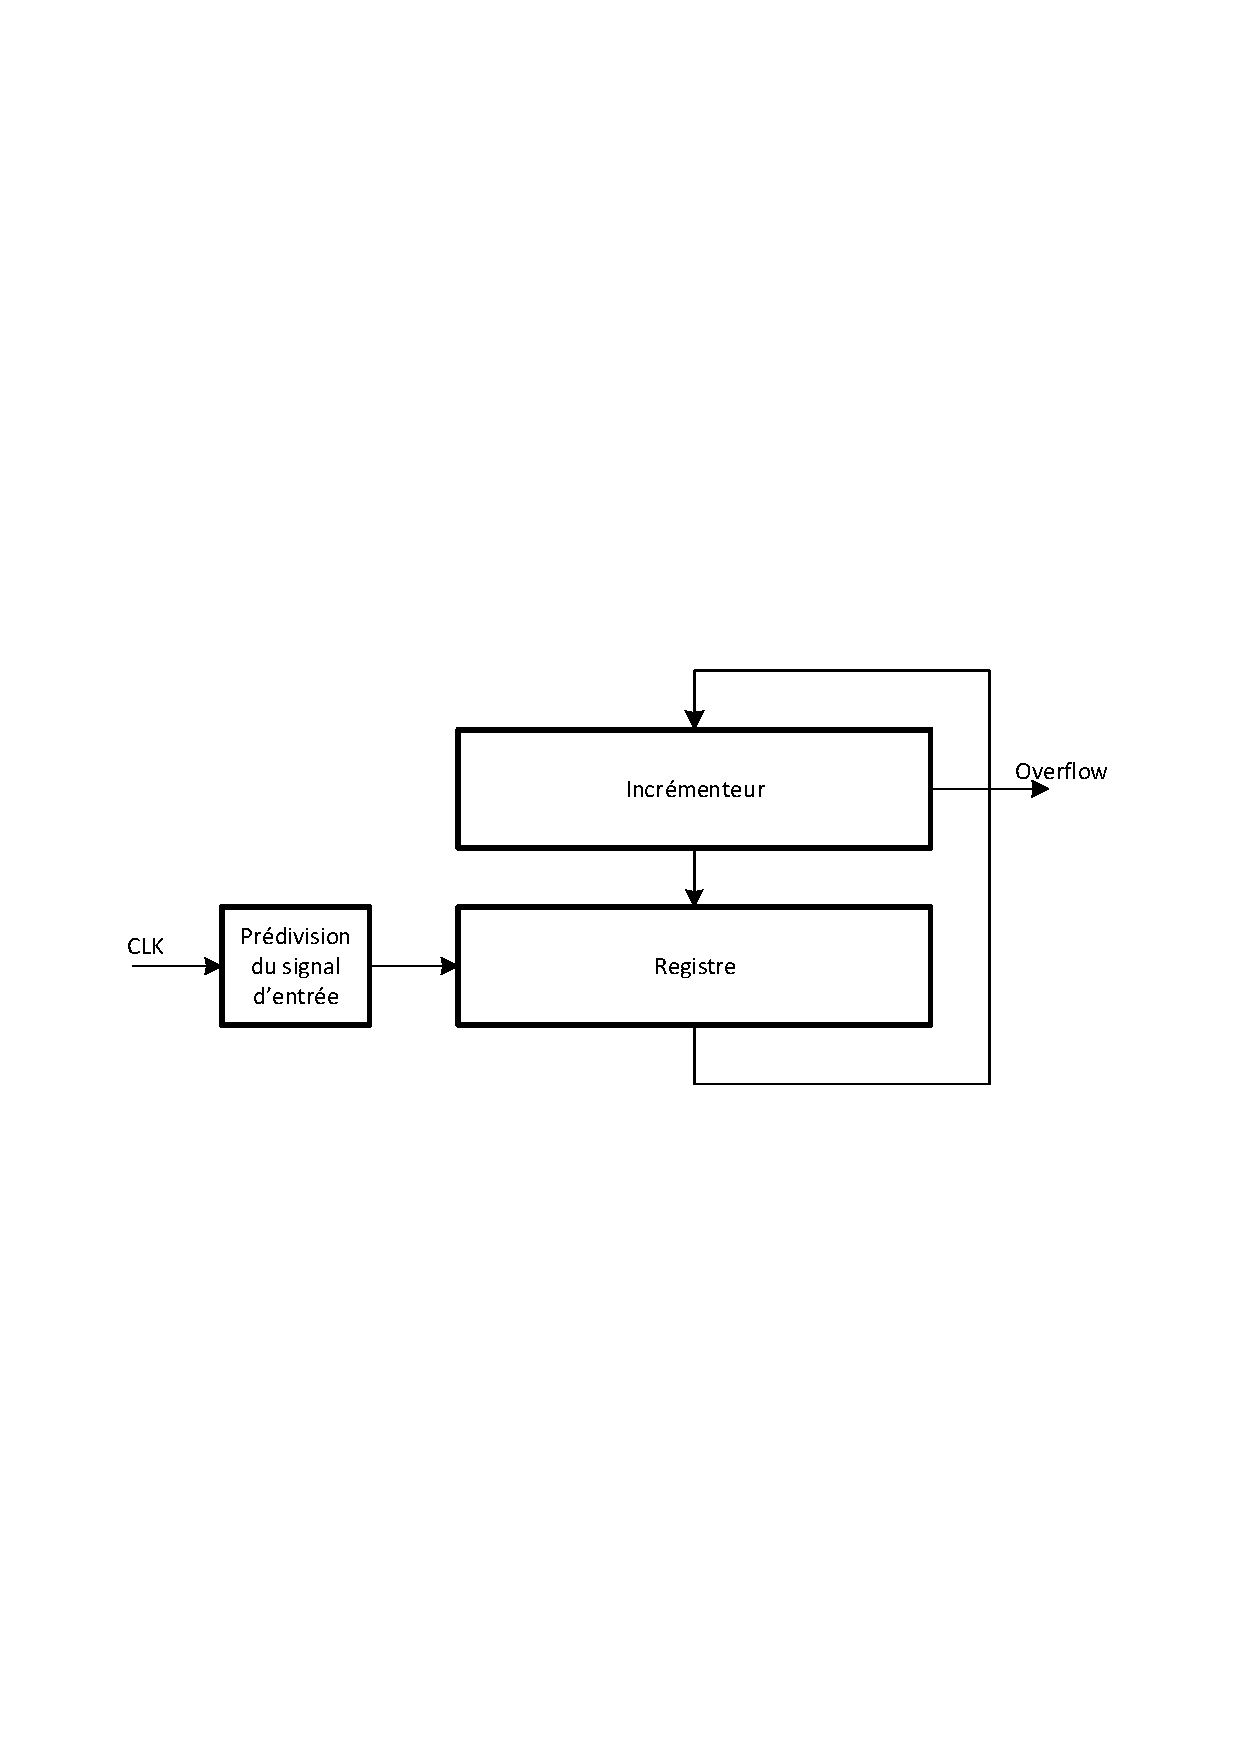
\includegraphics[angle=0, width=14cm]{./Figures/Chap5_Timer/Timer.pdf}
  \rule{35em}{0.5pt}
  \caption[Sch�ma Timer]{Sch�ma de base d'un timer}
  \label{fig:Timer}
\end{figure}

L'incr�mentation se fait au rythme d'un signal souvent appel� CLK (fig. \ref{fig:Timer}), qui est soit:
\begin{itemize}[label=\textbullet,font=\small]
\item p�riodique, auquel cas le circuit mesure (compte) le temps, et on parle de \textit{timer};
\item ap�riodique quelconque, auquel cas le circuit compte simplement les flancs de ce signal tant qu'il est actif et on parle plut�t de \textit{compteur}.
\end{itemize}

Souvent, un pr�diviseur de fr�quence permet de r�duire la fr�quence du signal CLK pour ralentir le rythme du comptage.

La figure \ref{fig:ChronoSync} montre l'�volution de la valeur du registre en fonction du temps, pour un \textit{timer} de 4 bits. La pente de la courbe d�pend du rythme auquel le registre est incr�ment�, donc de la fr�quence du signal CLK.
Lorsque le registre atteint sa valeur maximale, �gale � $2^N-1$, il repasse � 0. Durant ce passage � 0, un signal (qui est la retenue sortante du circuit incr�menteur) passe � '1' et �met �ventuellement une requ�te d'interruption.

\begin{figure}[htb]
  \centering
  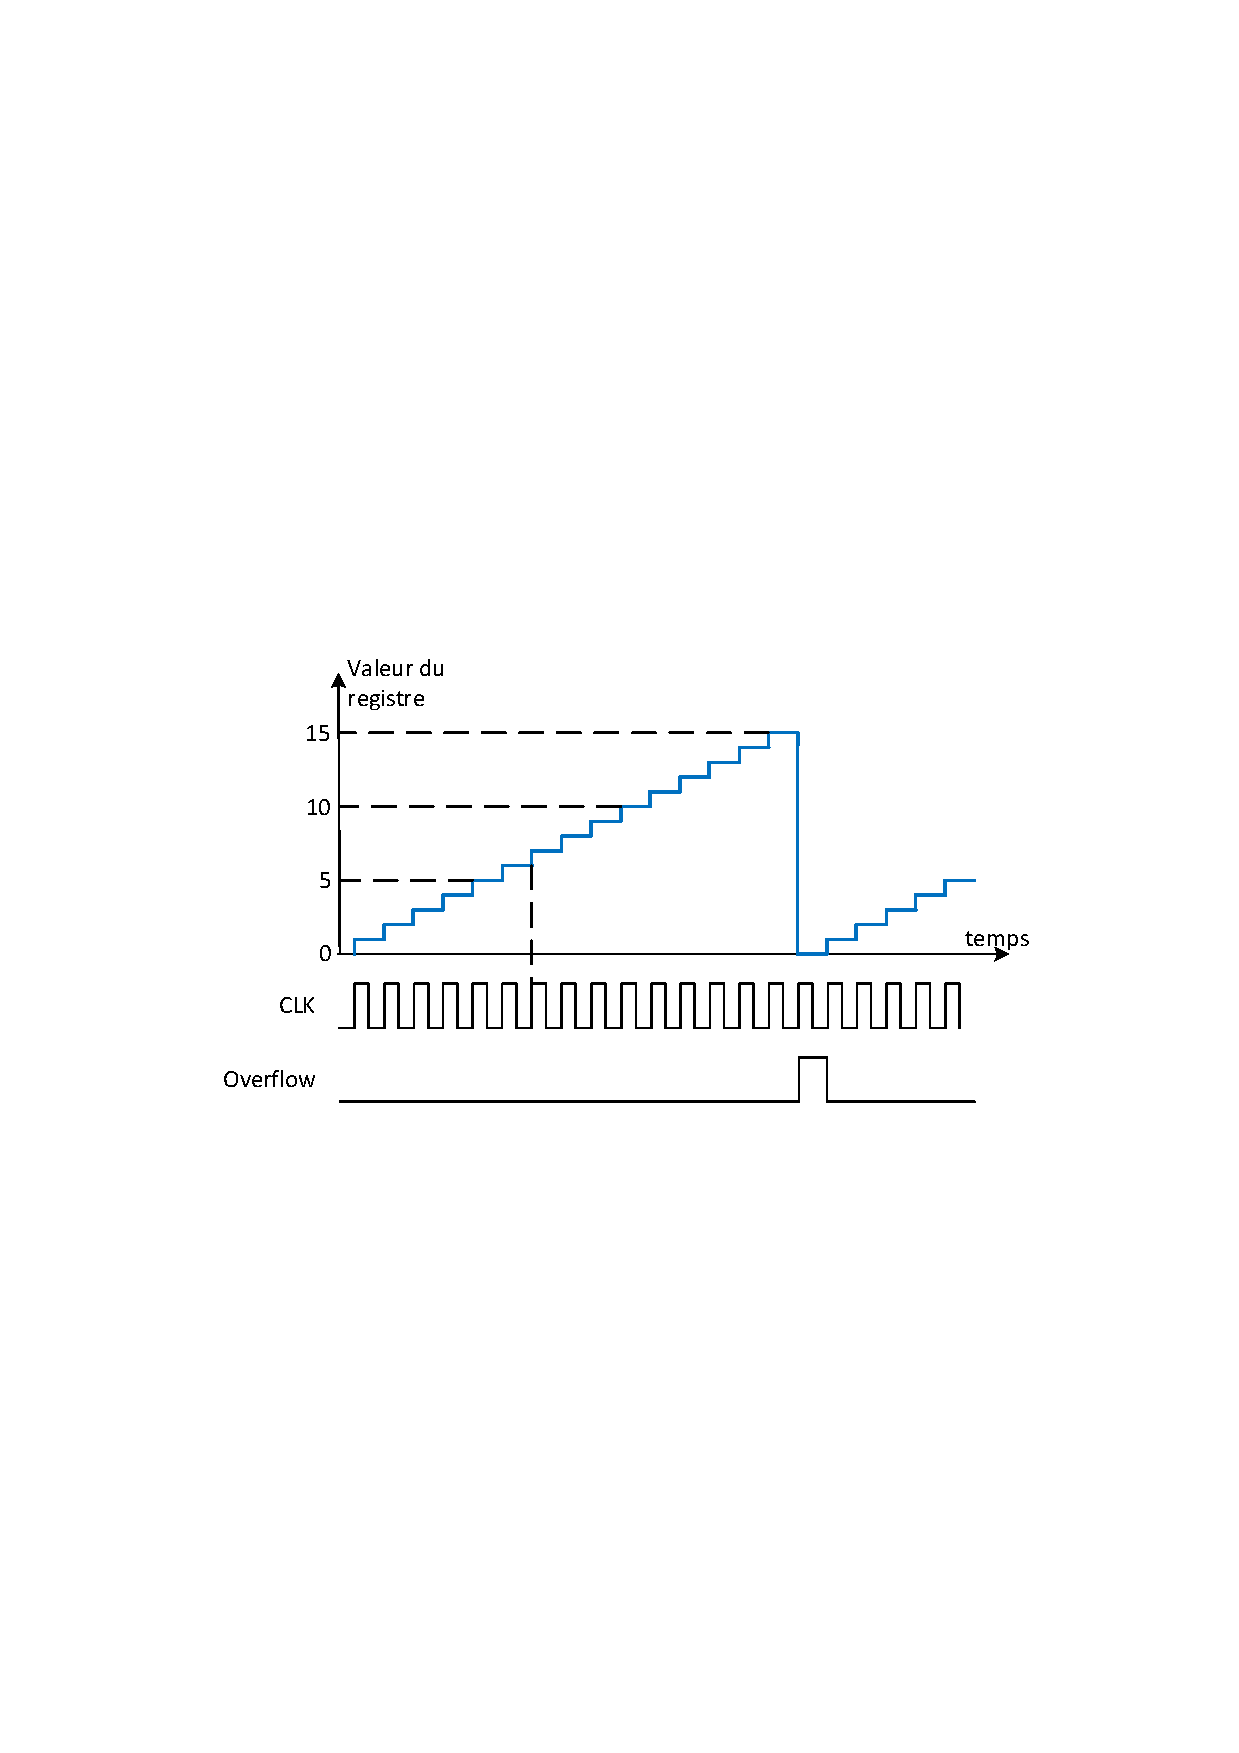
\includegraphics[angle=0, width=14cm]{./Figures/Chap5_Timer/Timer_chrono1.pdf}
  \rule{35em}{0.5pt}
  \caption[Chrono timer]{Comportement temporel du timer (N=4)}
  \label{fig:ChronoSync}
\end{figure}

Dans le cas d'un compteur, le signal CLK est ap�riodique. La figure \ref{fig:ChronoAsync} montre l'�volution de la valeur du registre en fonction du temps, pour un \textit{compteur} de 4 bits. De m�me, la retenue sortante du circuit incr�menteur�met �ventuellement une requ�te d'interruption lors du passage par 0 de la valeur du registre.

\begin{figure}[htb]
  \centering
  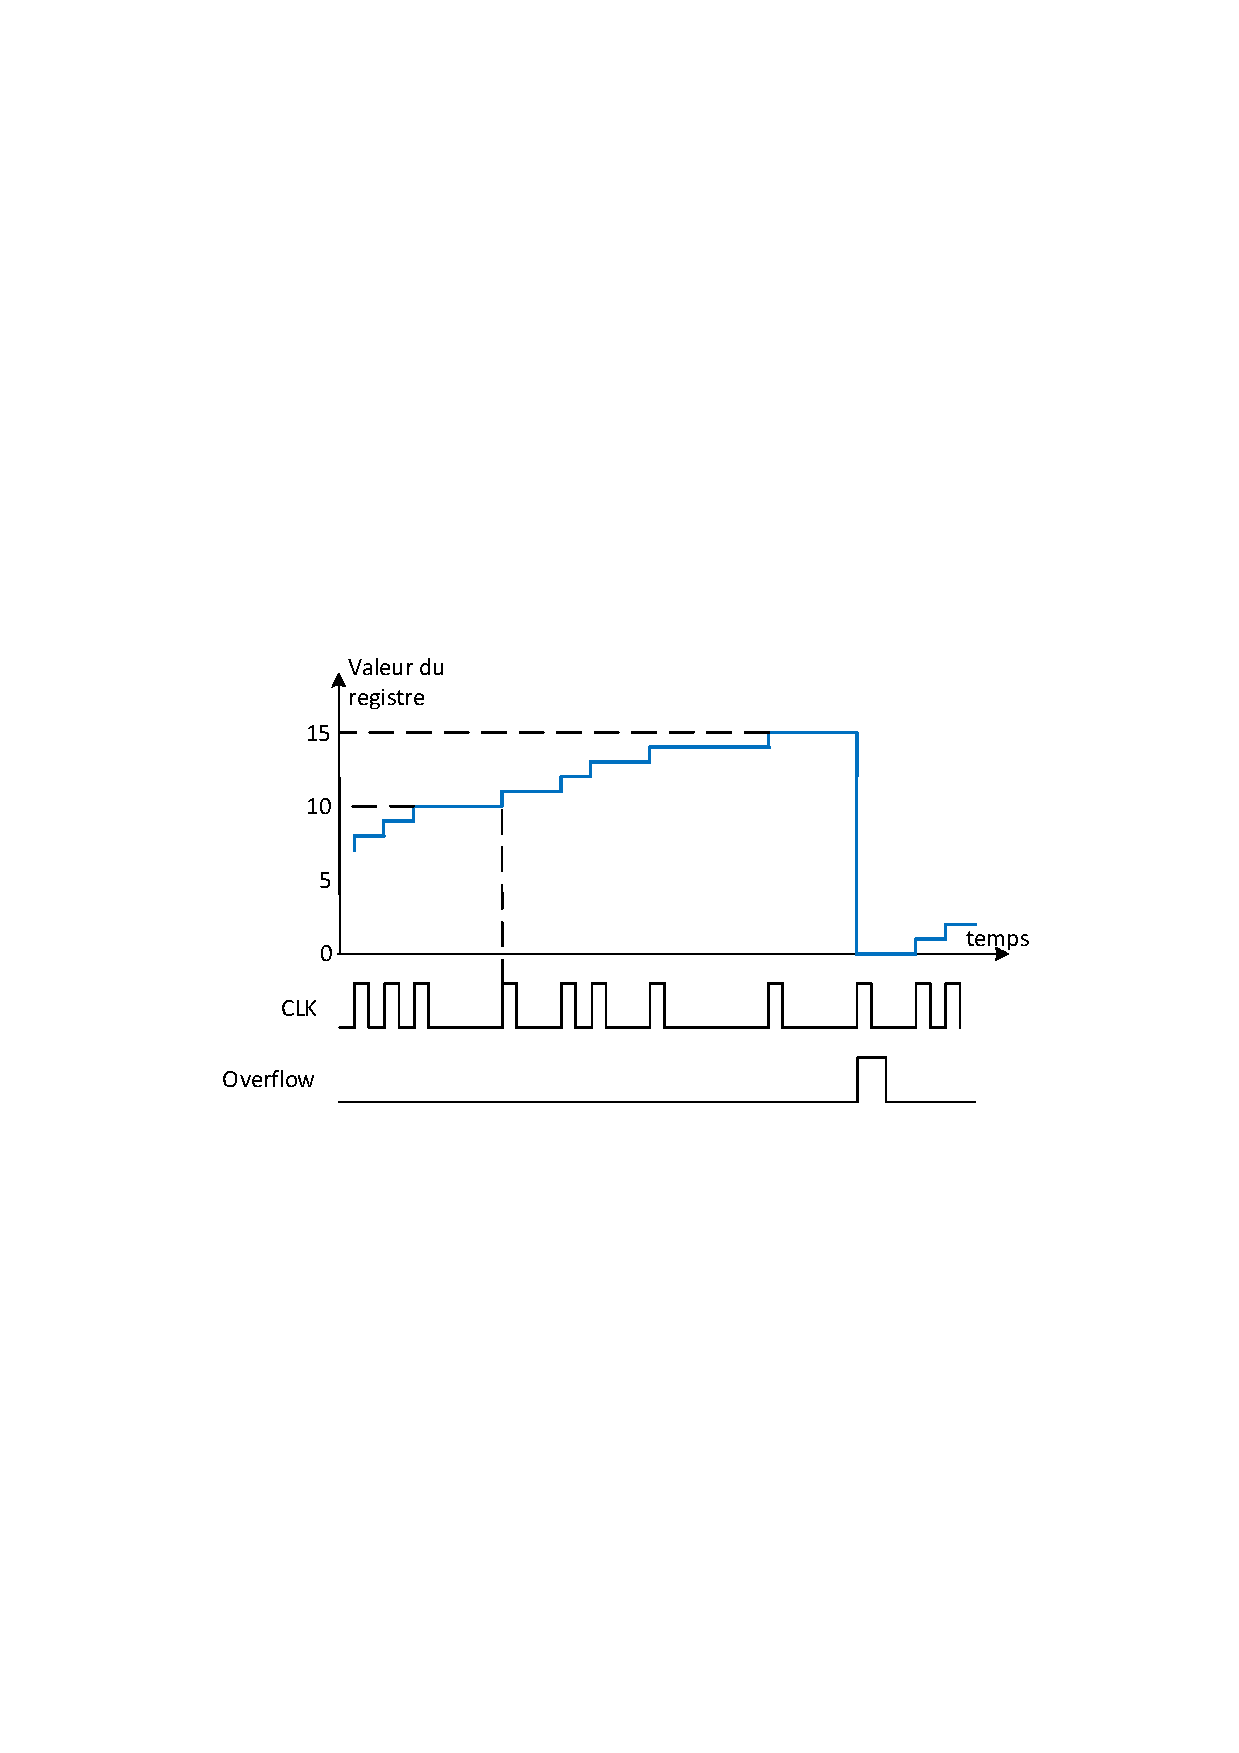
\includegraphics[angle=0, width=14cm]{./Figures/Chap5_Timer/Timer_chrono2.pdf}
  \rule{35em}{0.5pt}
  \caption[Chrono compteur]{Comportement temporel d'un compteur (N=4)}
  \label{fig:ChronoAsync}
\end{figure}

Comme nous le verrons dans la suite, certains timers utilisent un d�cr�menteur au lieu d'un incr�menteur, voire les deux.
Finalement, on peut rencontrer diff�rents types de timers dans un m�me microcontr�leur, chacun �tant adapt� � un besoin sp�cifique.

\section{Cas du MSP430}
Les microcontr�leurs de la famille MSP430 embarquent jusqu'� 4 types de timers diff�rents:
\begin{itemize}[label=\textbullet,font=\small]
\item Real Time Clock, ou \textit{Horloge Temps R�el} (RTC) pour la cr�ation d'horloges
\item WatchDog Timer ou \textit{Chien de Garde} (WDT) pour la pr�vention de plant�es d'origines diverses
\item Timers � usage g�n�ral
\end{itemize}

\subsection{Real Time Clock}
Apr�s initialisation, le RTC maintient � jour les informations horaires les plus courantes :
\begin{itemize}[label=\textbullet,font=\small]
\item ann�e
\item num�ro du mois dans l'ann�e
\item jour du mois
\item jour de la semaine
\item heure
\item minute
\item seconde
\end{itemize}

Ce type de timer n�cessite une horloge dont la fr�quence est 1Hz, d�riv�e d'une horloge standard � 32768Hz. Cette derni�re fr�quence fut introduite aux d�buts de la montre � quartz car il est ais� de r�aliser des quartz � cette fr�quence. On obtient l'horloge � 1Hz par une simple division de 32768 par $2^{15}$.

\subsection{WatchDog Timer}
La "plant�e" d'un programme est la plupart du temps due � un d�faut dans le programme ou � un concours de circonstances qui fait que le programme est bloqu� dans un boucle sans fin. Le cas le plus courant est l'attente d'un �v�nement qui n'arrive pas et qui n'arrivera jamais.
Le microcontr�leur ne r�agit plus. Le seul moyen est de le \textit{resetter}.

\section{Timer � usage g�n�ral : le timer A}
Dans le MSP430, le timer � usage g�n�ral est un p�riph�rique complexe auquel le CPU peut soutraiter des fonctionnalit�s sophistiqu�es. En plus des fonctionnalit�s usuelles, on trouve:
\begin{itemize}[label=\textbullet,font=\small]
\item capture de l'�tat du registre de comptage lors d'un �v�nement
\item requ�tes d'interruption d�s que le registre de comptage a atteint une constante donn�e (comparaison)
\item g�n�ration de signaux PWM sur une patte externe, sans aucune aide du CPU autre que l'initialisation
\end{itemize}
Toutes ces fonctionnalit�s sont contr�l�es par le logiciel, en positionnant des champs logiques dans des registres de contr�le. champ logique est un groupe de variables logiques dans un registre.

Dans une version de MSP430 donn�e, plusieurs Timers A peuvent coexister.

La figure \ref{fig:TimerAsimplifie} est un sch�ma tr�s simplifi� du timer A, illustrant ses 3 principaux sous-blocs.

\begin{figure}[htb]
  \centering
  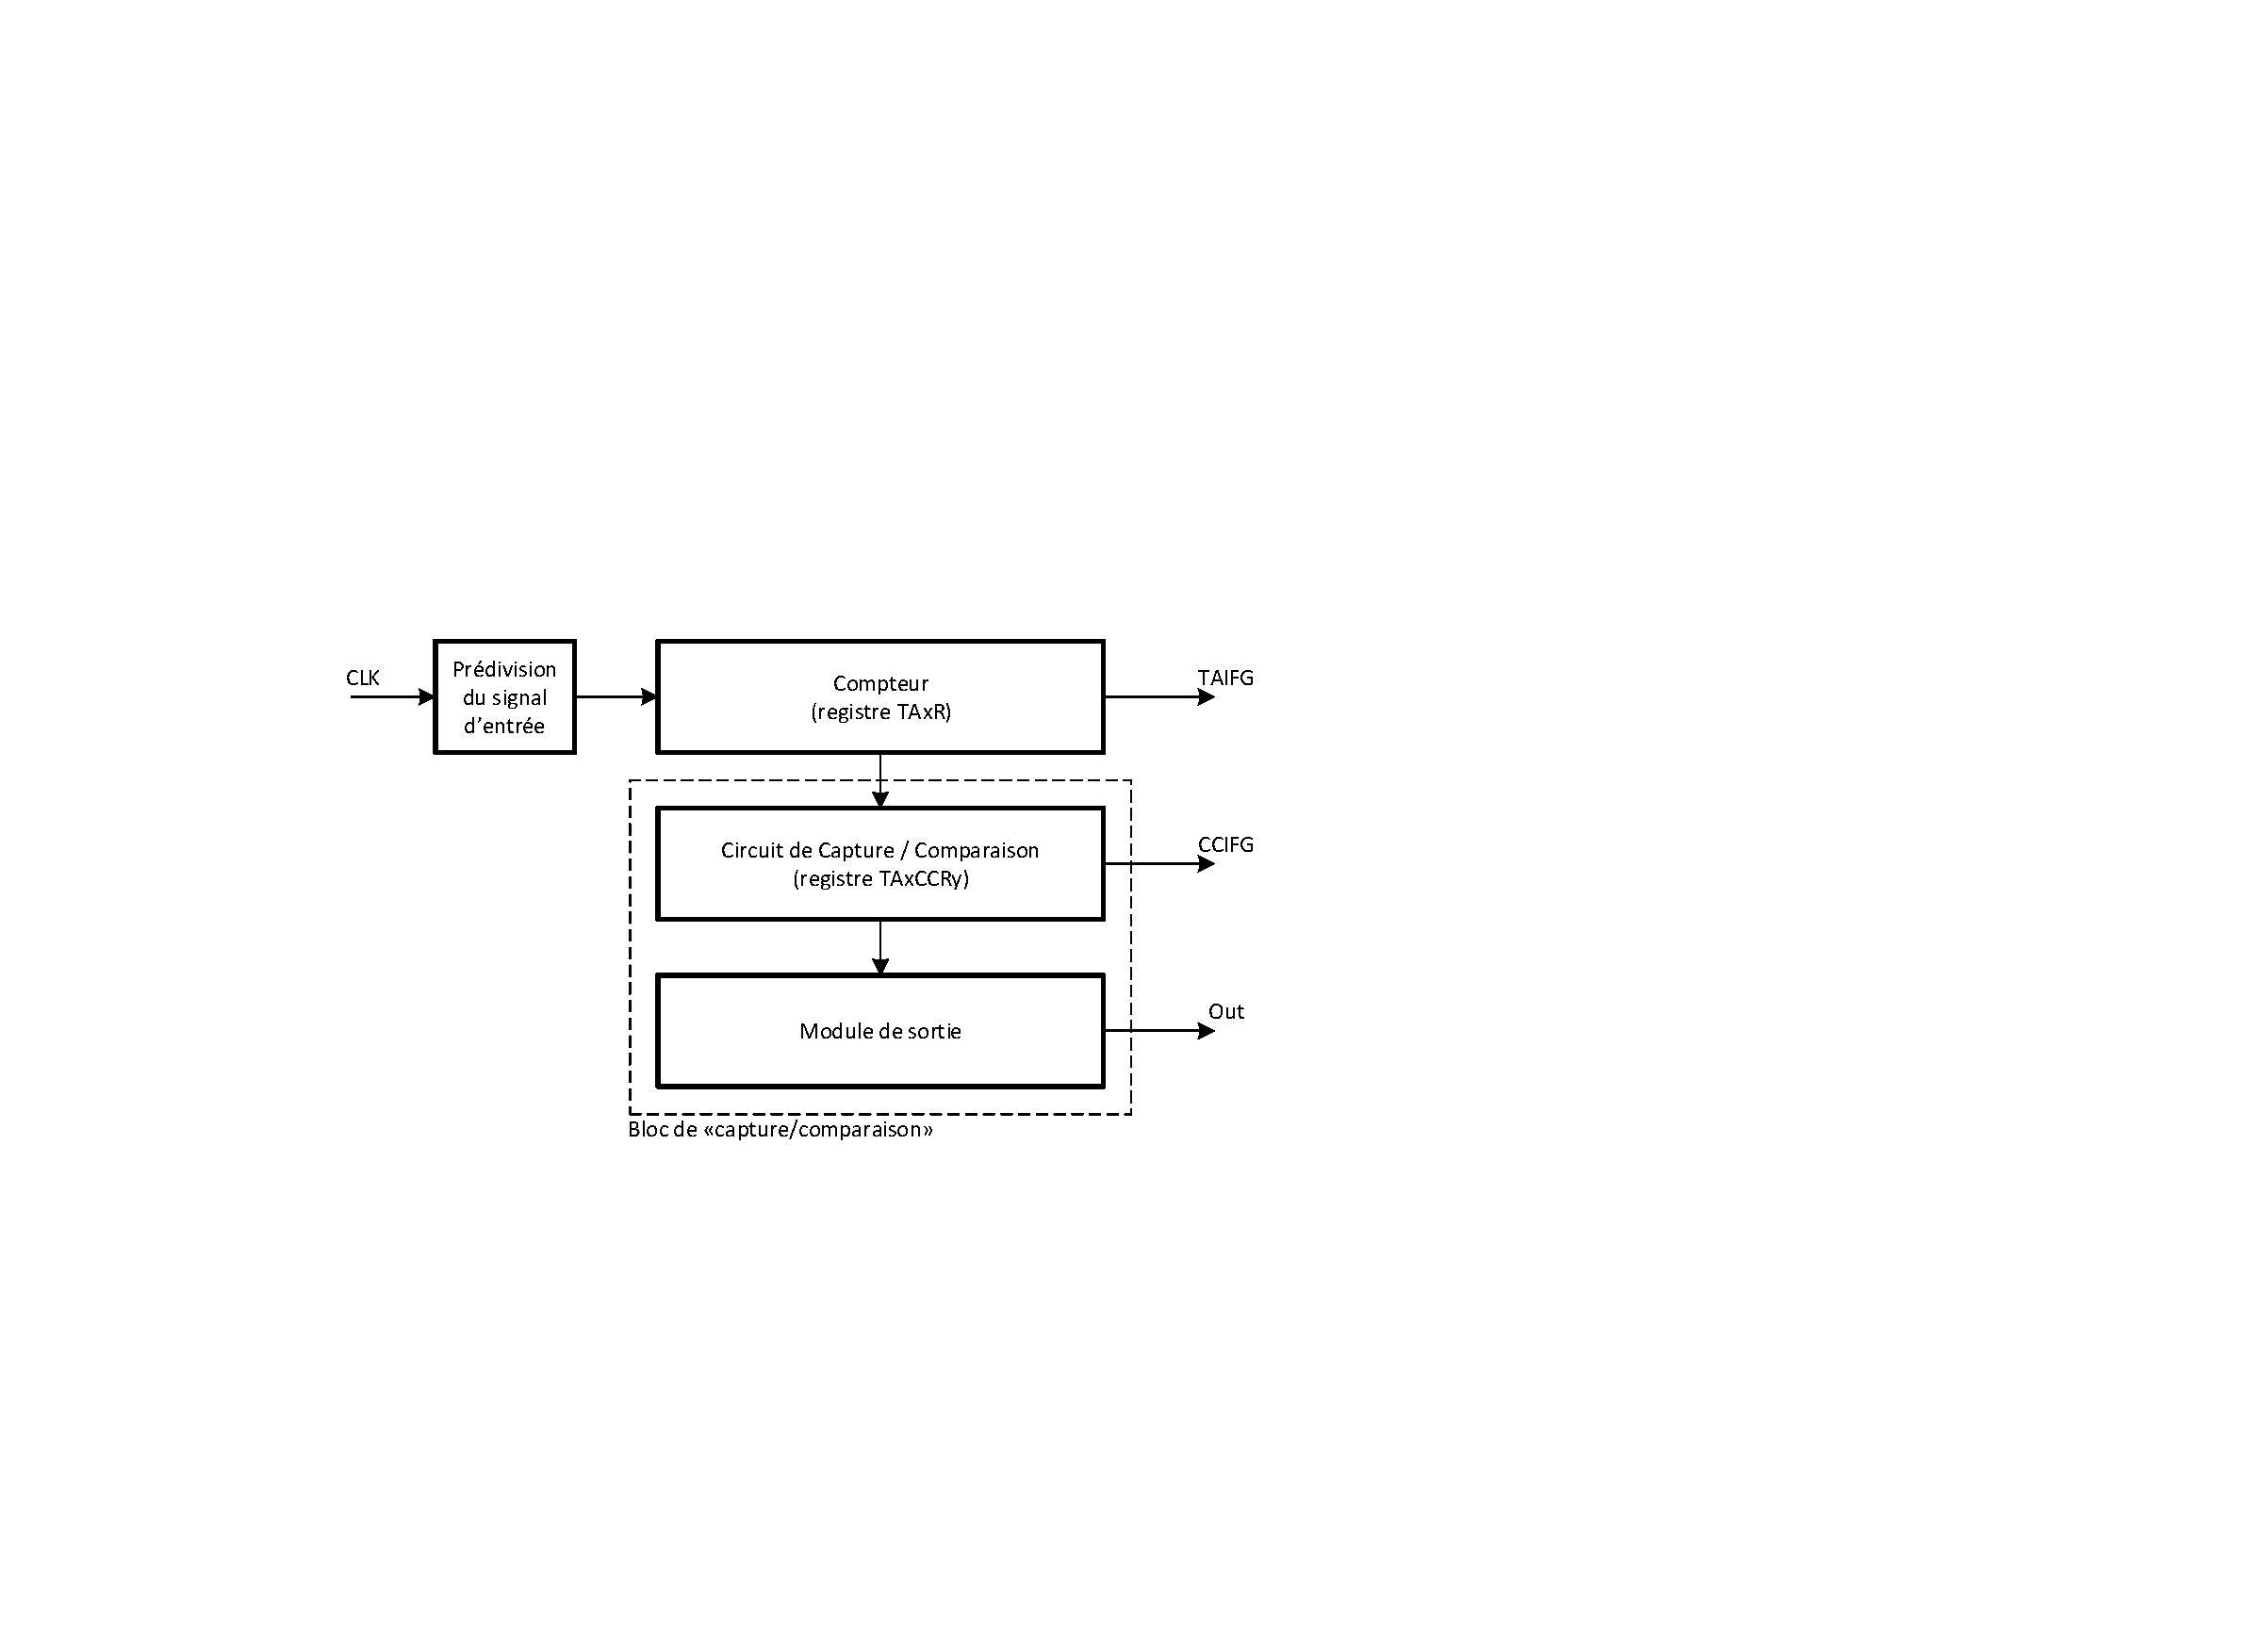
\includegraphics[angle=0, width=14cm]{./Figures/Chap5_Timer/Timer_blocs_1.pdf}
  \rule{35em}{0.5pt}
  \caption[TimerA simplifie]{Sch�ma simplifi� du timer A}
  \label{fig:TimerAsimplifie}
\end{figure}

A la partie sup�rieure, on retrouve le bloc de comptage et son registre appel� TAxR (x est le num�ro du timer; x=0 ou 1 s'il y a deux timers de type A dans le microcontr�leur). TAIFG est le signal d'overflow du compteur. En dessous, le bloc dit de "capture/comparaison" permet de capturer l'�tat du registre TAxR lors d'un �v�nement ou de comparer la valeur de TAxR avec une constante contenue dans un registre appel� TAxCCRy. Le bloc de "capture/comparaison" contient un sous-bloc, not� "Output module", qui est charg� de g�n�rer un signal PWM � partir du contenu du registre TAxR et de la constante contenue dans le registre TAxCCRy. 

Pour enrichir encore les possibilit�s offertes par le timer A, celui-ci dispose de plusieurs blocs de "capture/comparaison". Selon le type de microcontr�leur, le timer A dispose de 3, 5 ou 7 de ces blocs. Nous y reviendrons ult�rieurement.

\subsection{Modes de comptage}
Le registre de comptage TAxR a 3 modes de comptage possibles. Le mode est d�termin� par la valeur du champ MCx dans le registre de contr�le TACTLx:
\begin{itemize}[label=\textbullet,font=\small]
\item Mode 1 (MCx = 01): Comptage jusqu'� la valeur contenue dans le registre TAxCCR0, localis� dans un sous-bloc de capture/comparaison, puis retour � 0;
\item Mode 2 (MCx = 10): Comptage jusqu'� 0xFFFF, puis retour � 0;
\item Mode 3 (MCx = 11): Comptage jusqu'� la valeur contenue dans le registre TAxCCR0, puis d�comptage jusqu'� 0.
\end{itemize}

Les figures \ref{fig:TimerAmode1}, \ref{fig:TimerAmode2} et \ref{fig:TimerAmode3a} montrent les chronogrammes associ�s � chaque mode.
\begin{figure}[htb]
  \centering
  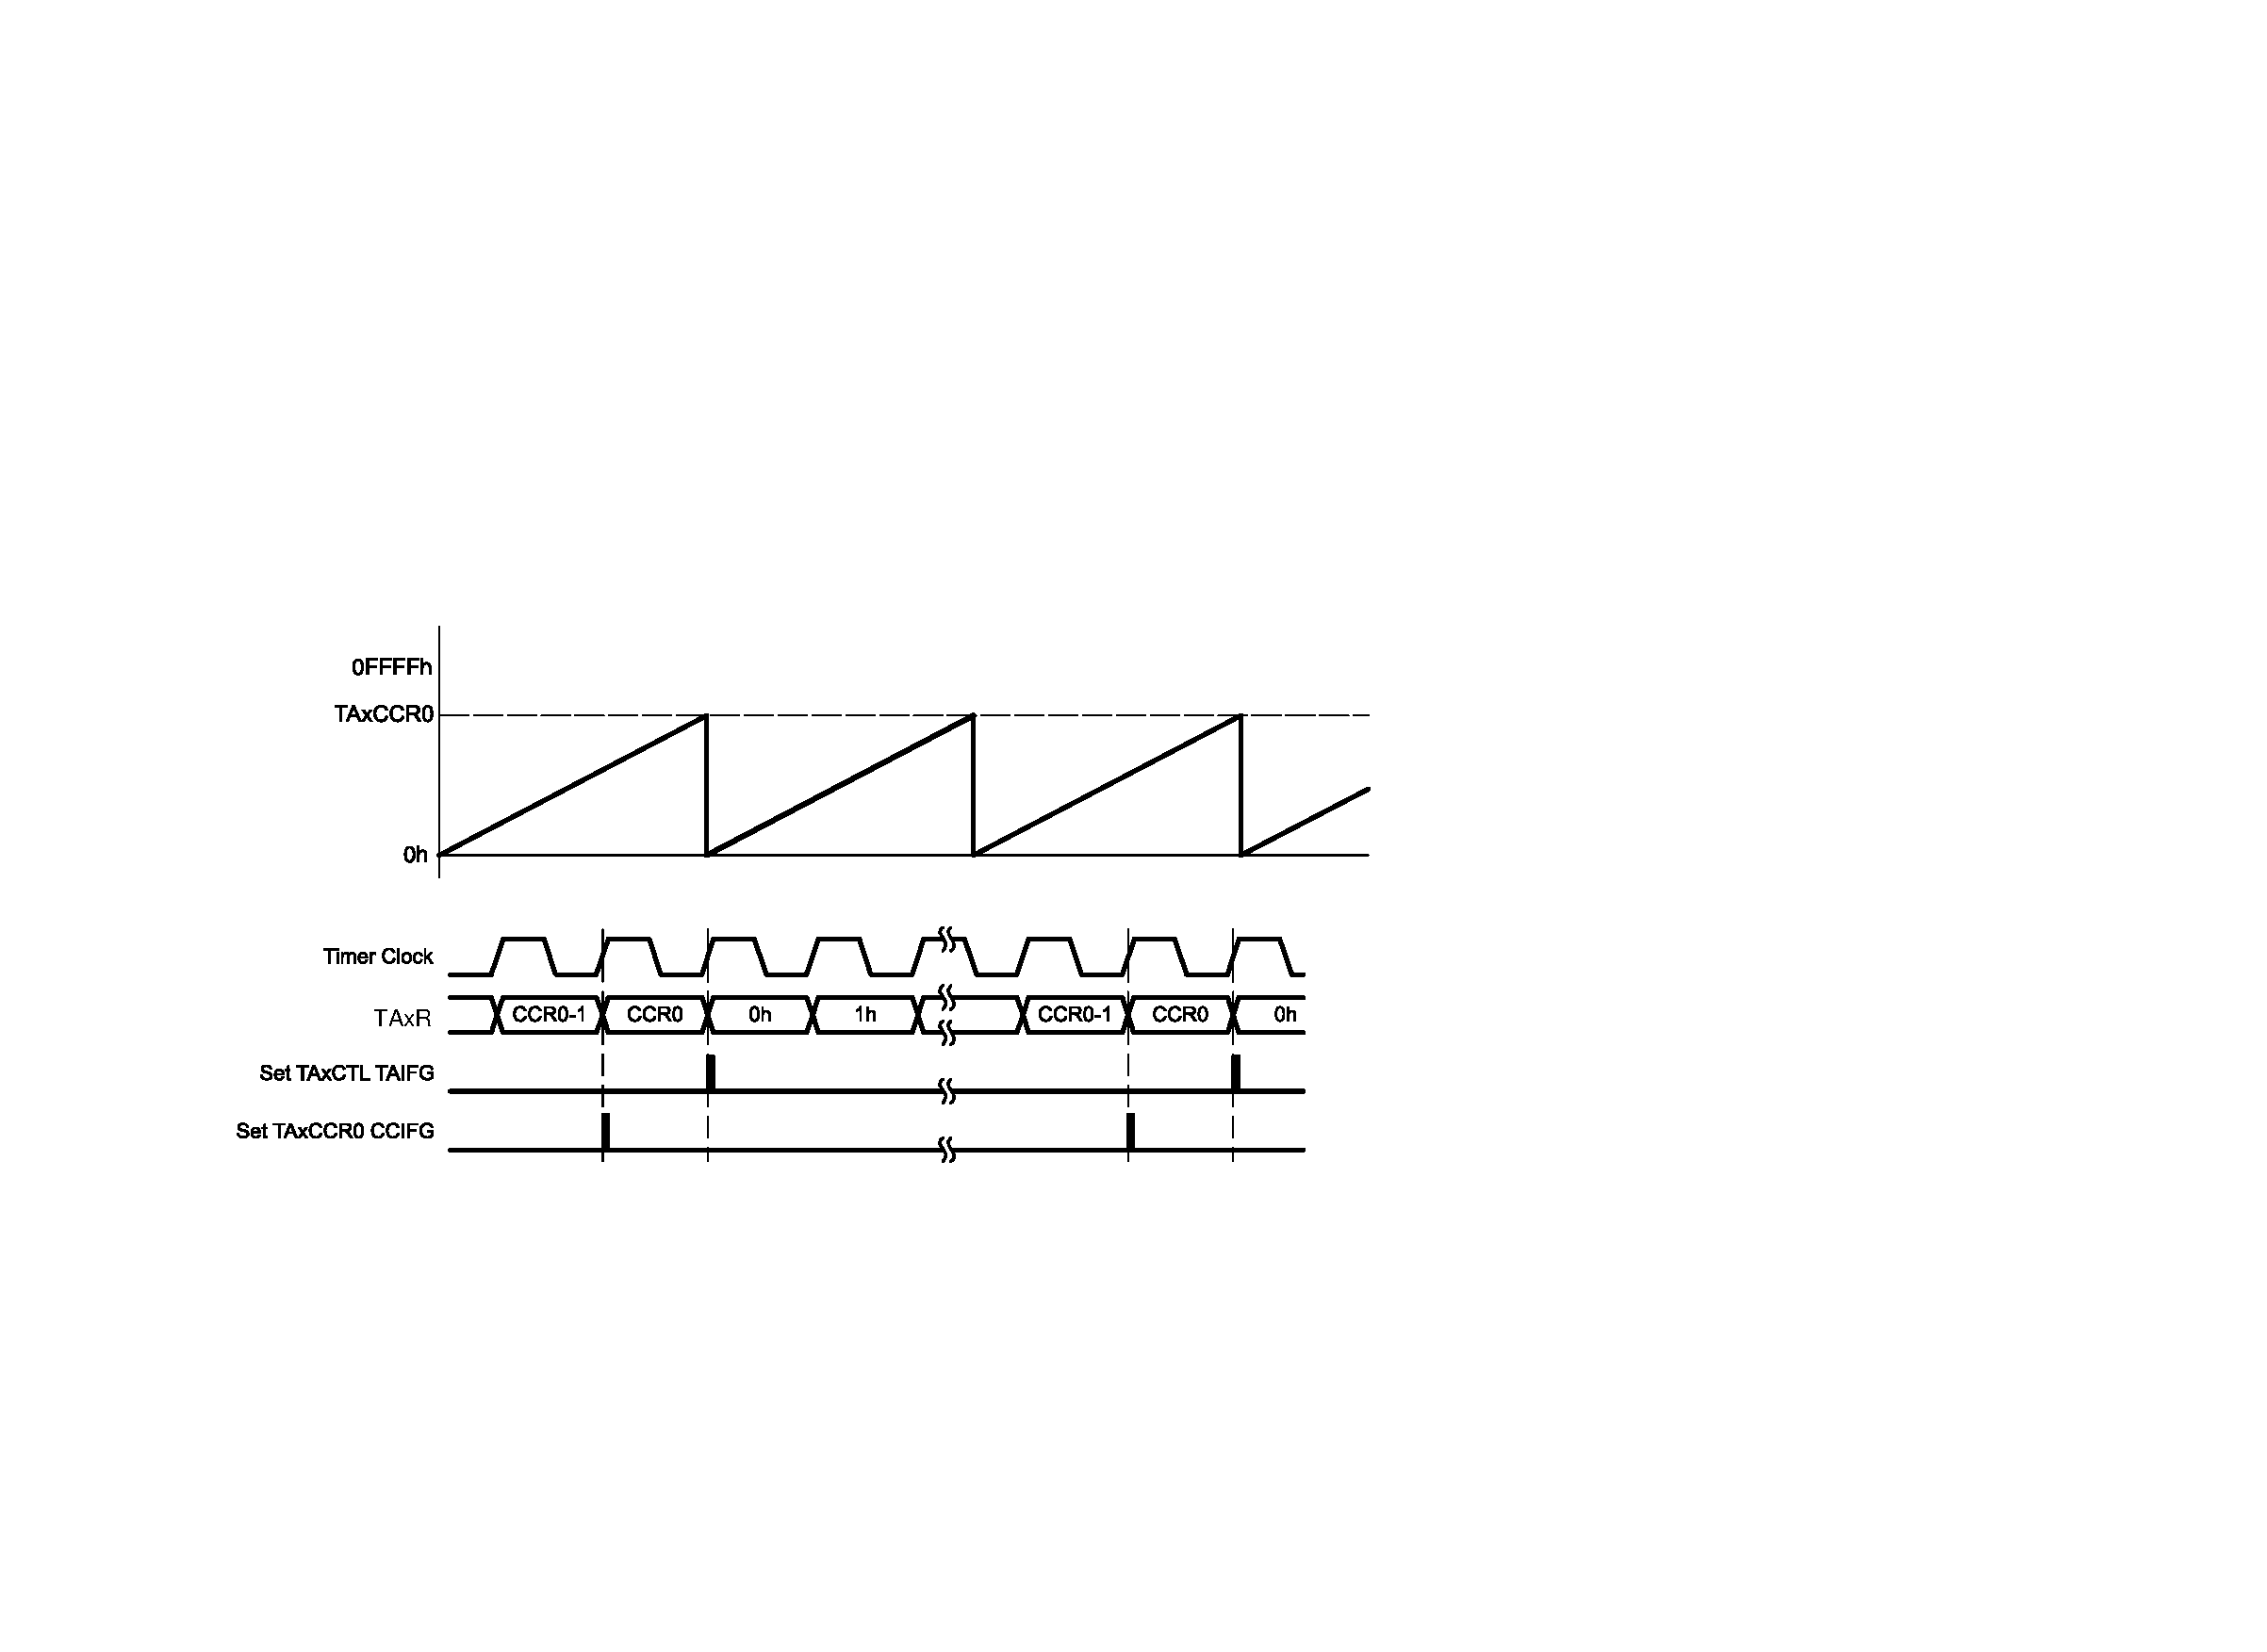
\includegraphics[angle=0, width=14cm]{./Figures/Chap5_Timer/Timer_Mode_1.pdf}
  \rule{35em}{0.5pt}
  \caption[TimerA Mode 1]{Comptage en mode 1 (MCx = 01)}
  \label{fig:TimerAmode1}
\end{figure}

\begin{figure}[htb]
  \centering
  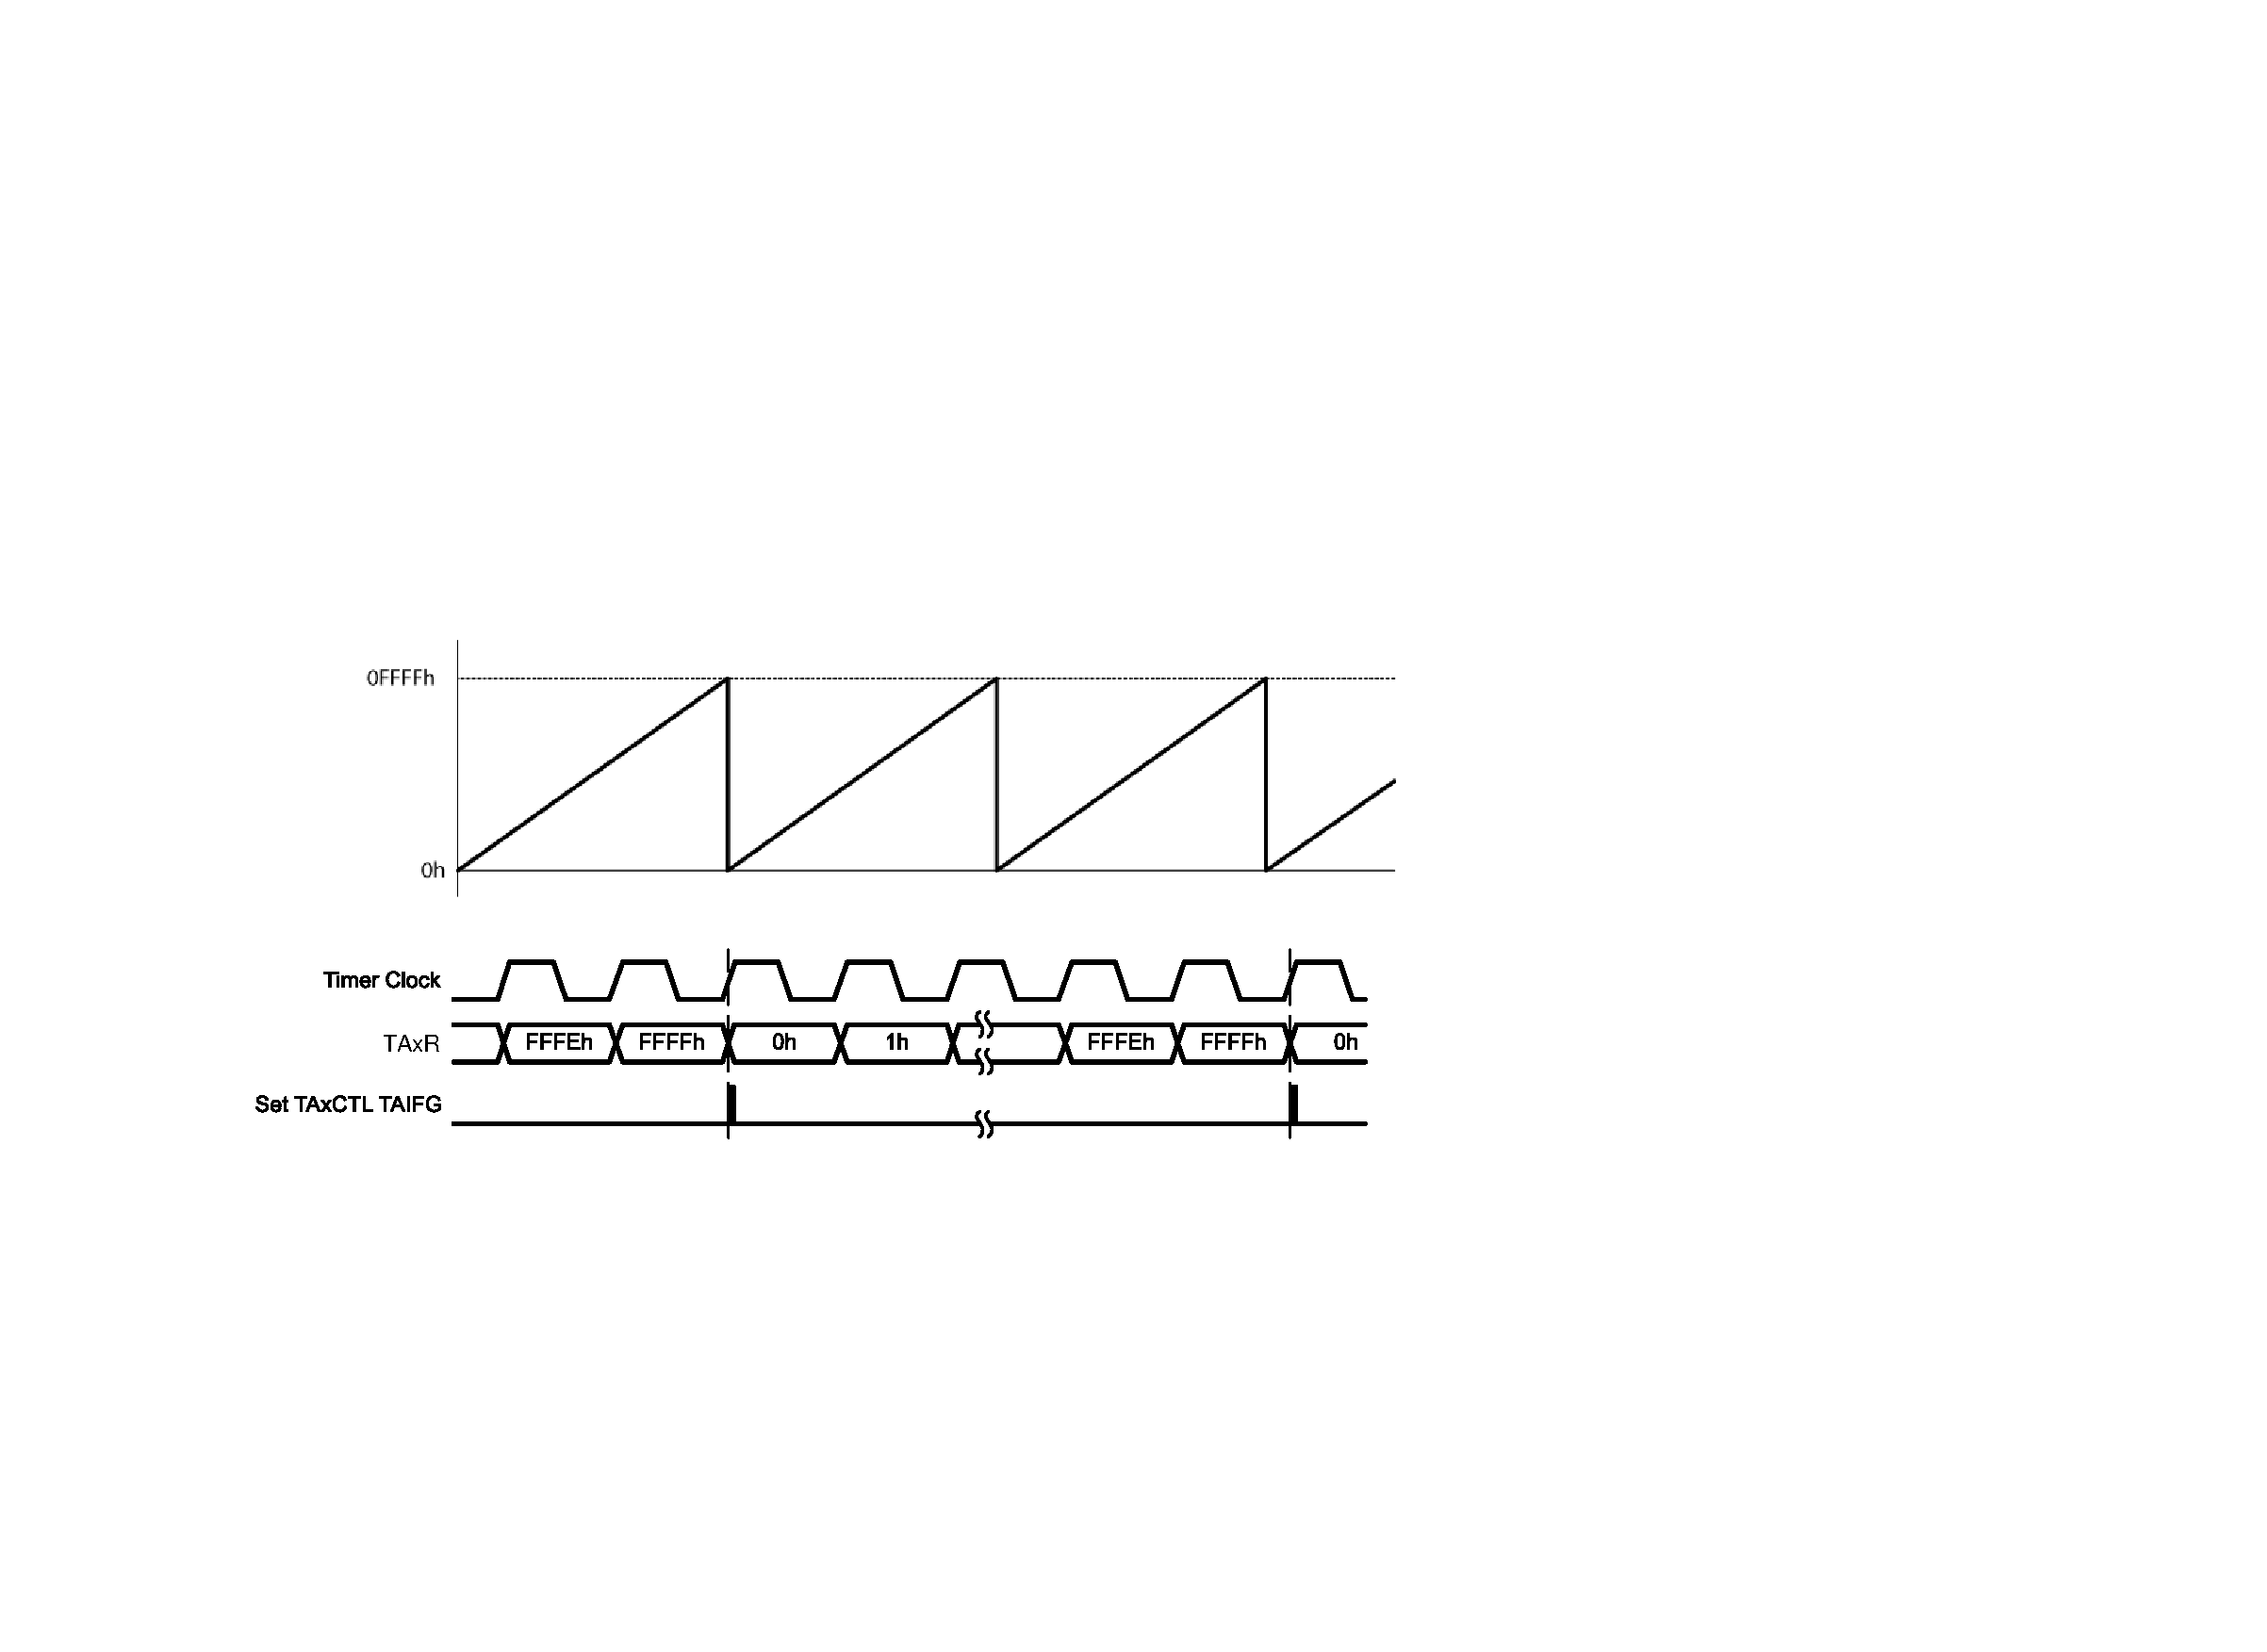
\includegraphics[angle=0, width=14cm]{./Figures/Chap5_Timer/Timer_Mode_2.pdf}
  \rule{35em}{0.5pt}
  \caption[TimerA Mode 2]{Comptage en mode 2 (MCx = 10)}
  \label{fig:TimerAmode2}
\end{figure}

\begin{figure}[htb]
  \centering
  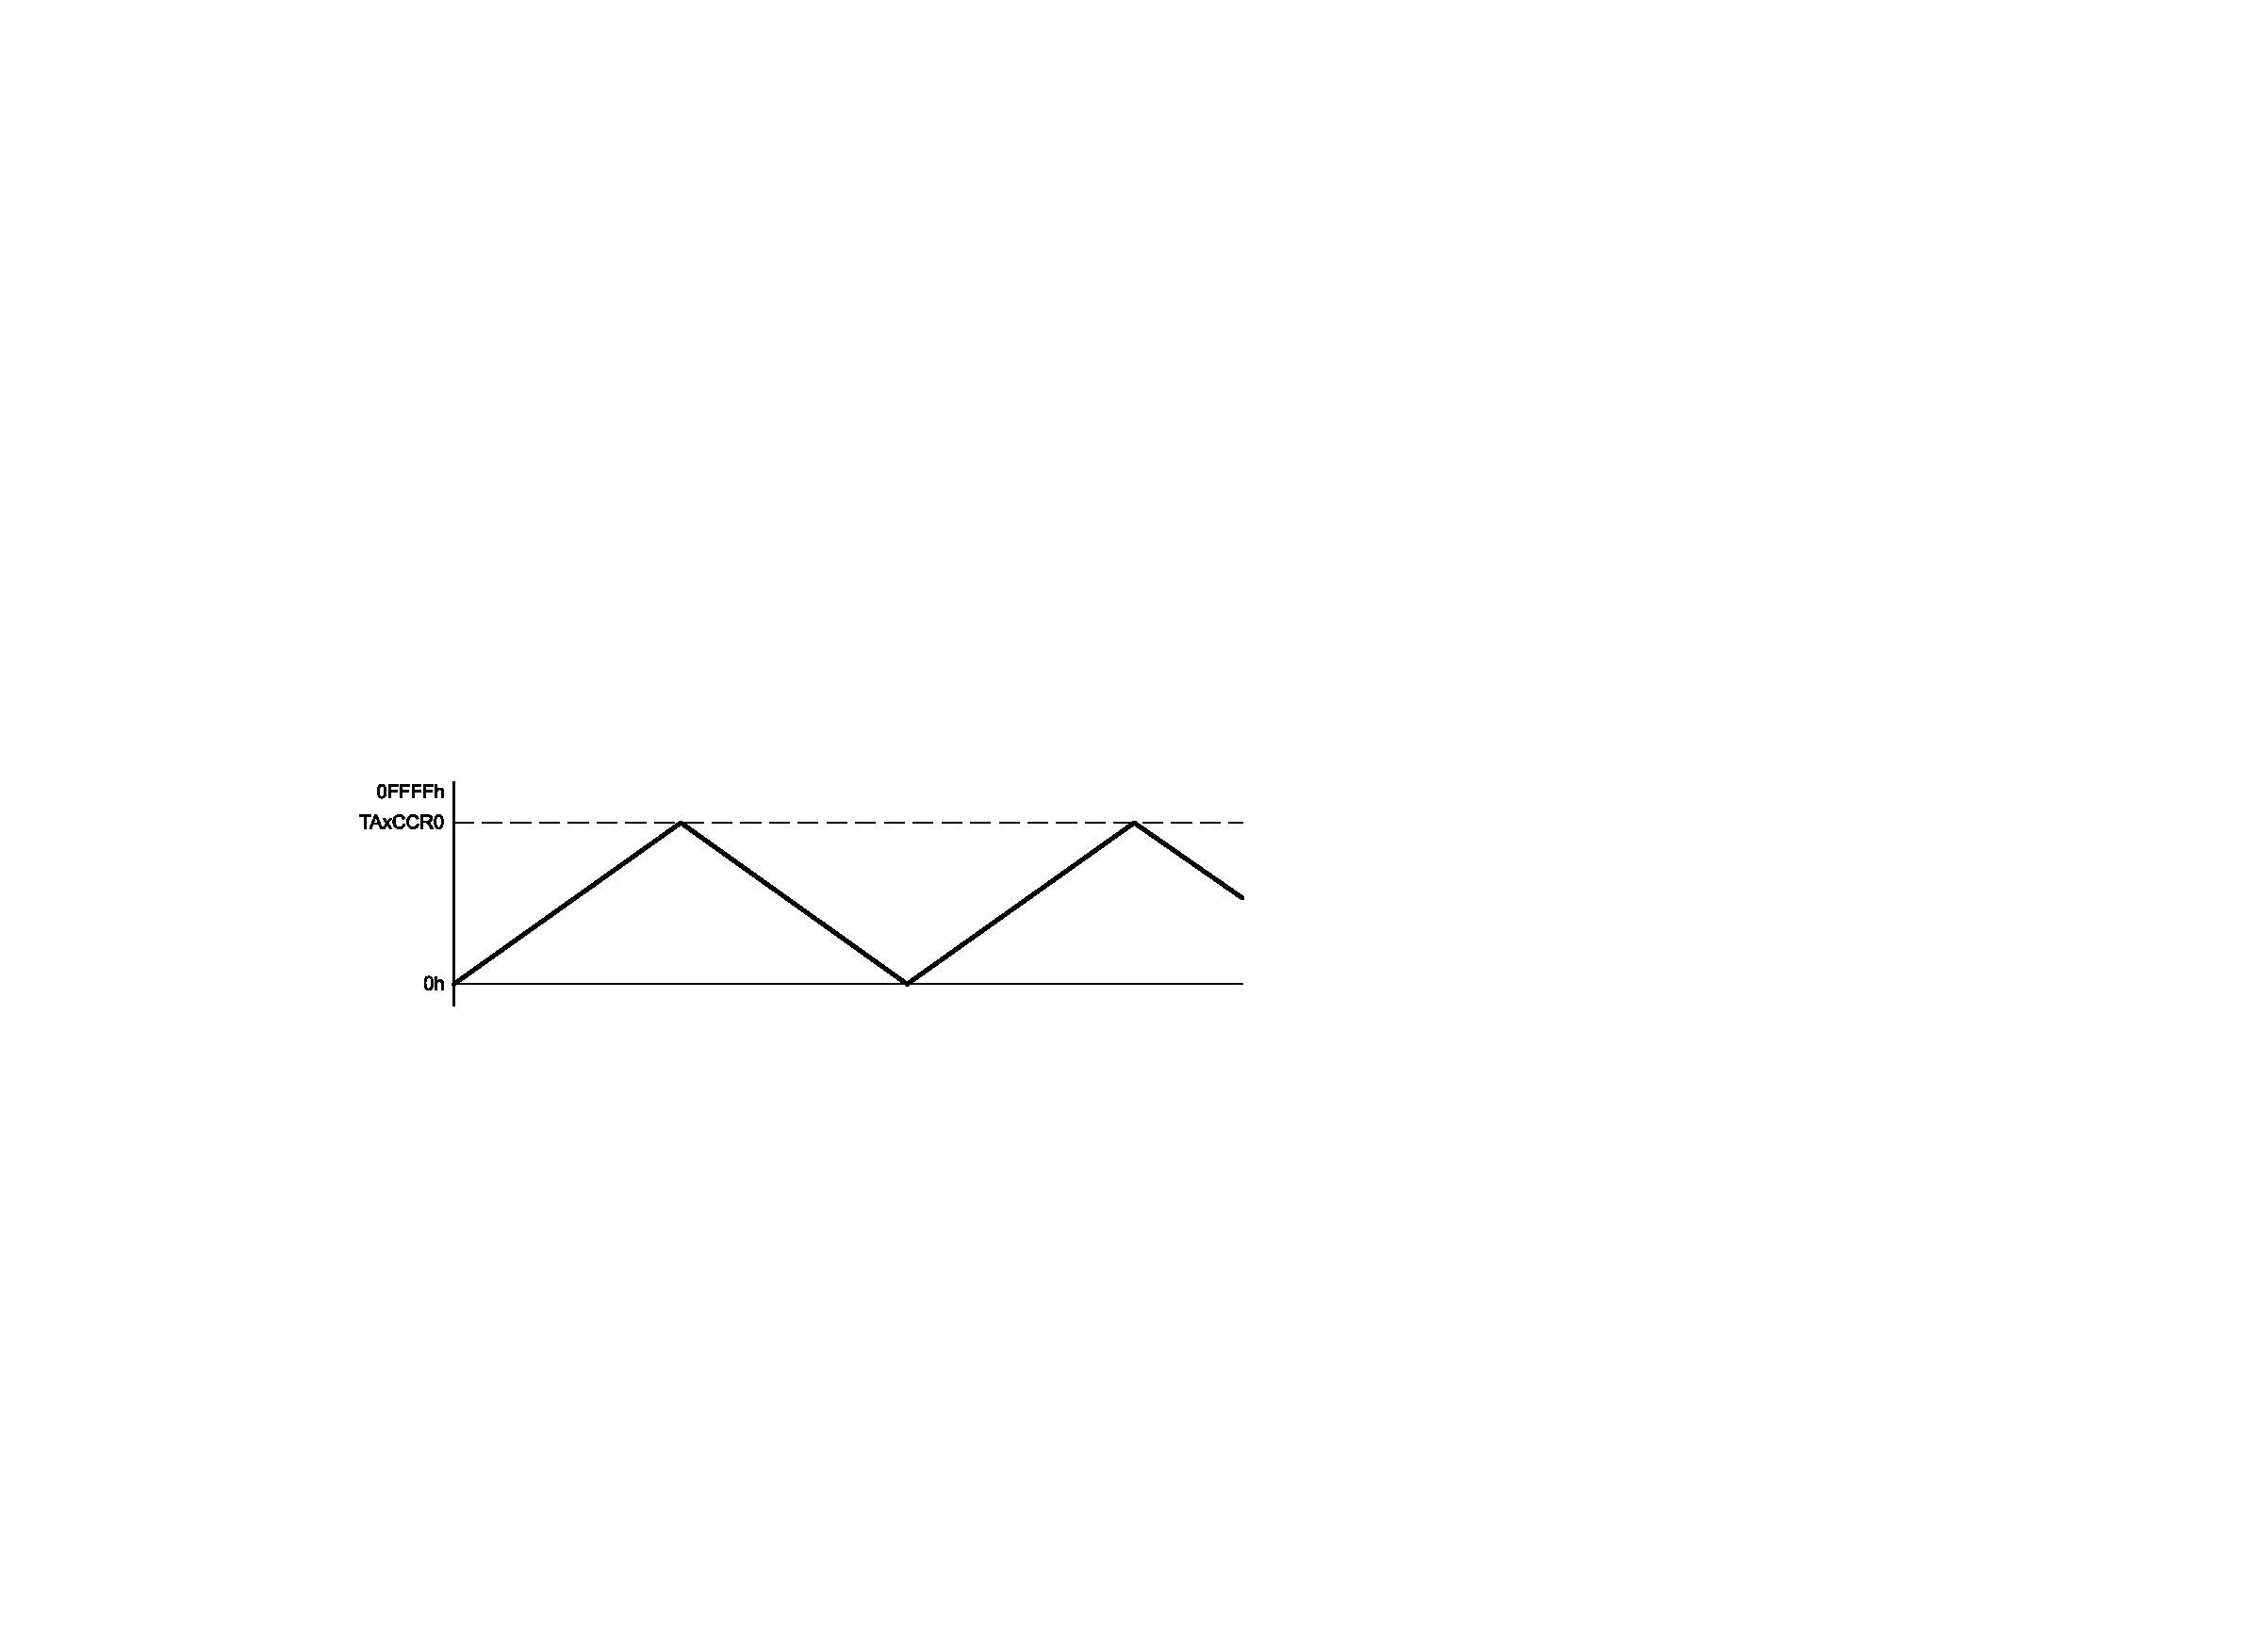
\includegraphics[angle=0, width=12cm]{./Figures/Chap5_Timer/Timer_Mode_3a.pdf}
  \rule{35em}{0.5pt}
  \caption[TimerA Mode 3]{Comptage en mode 3 (MCx = 11)}
  \label{fig:TimerAmode3a}
\end{figure}

Dans le cas du mode 3, la figure  \ref{fig:TimerAmode3b} pr�cise le comportement des signaux TAIFG et du signal de sortie CCIFG du bloc de capture/comparaison n�0 (celui qui contient le registre TAxCCR0).
\begin{figure}[htb]
  \centering
  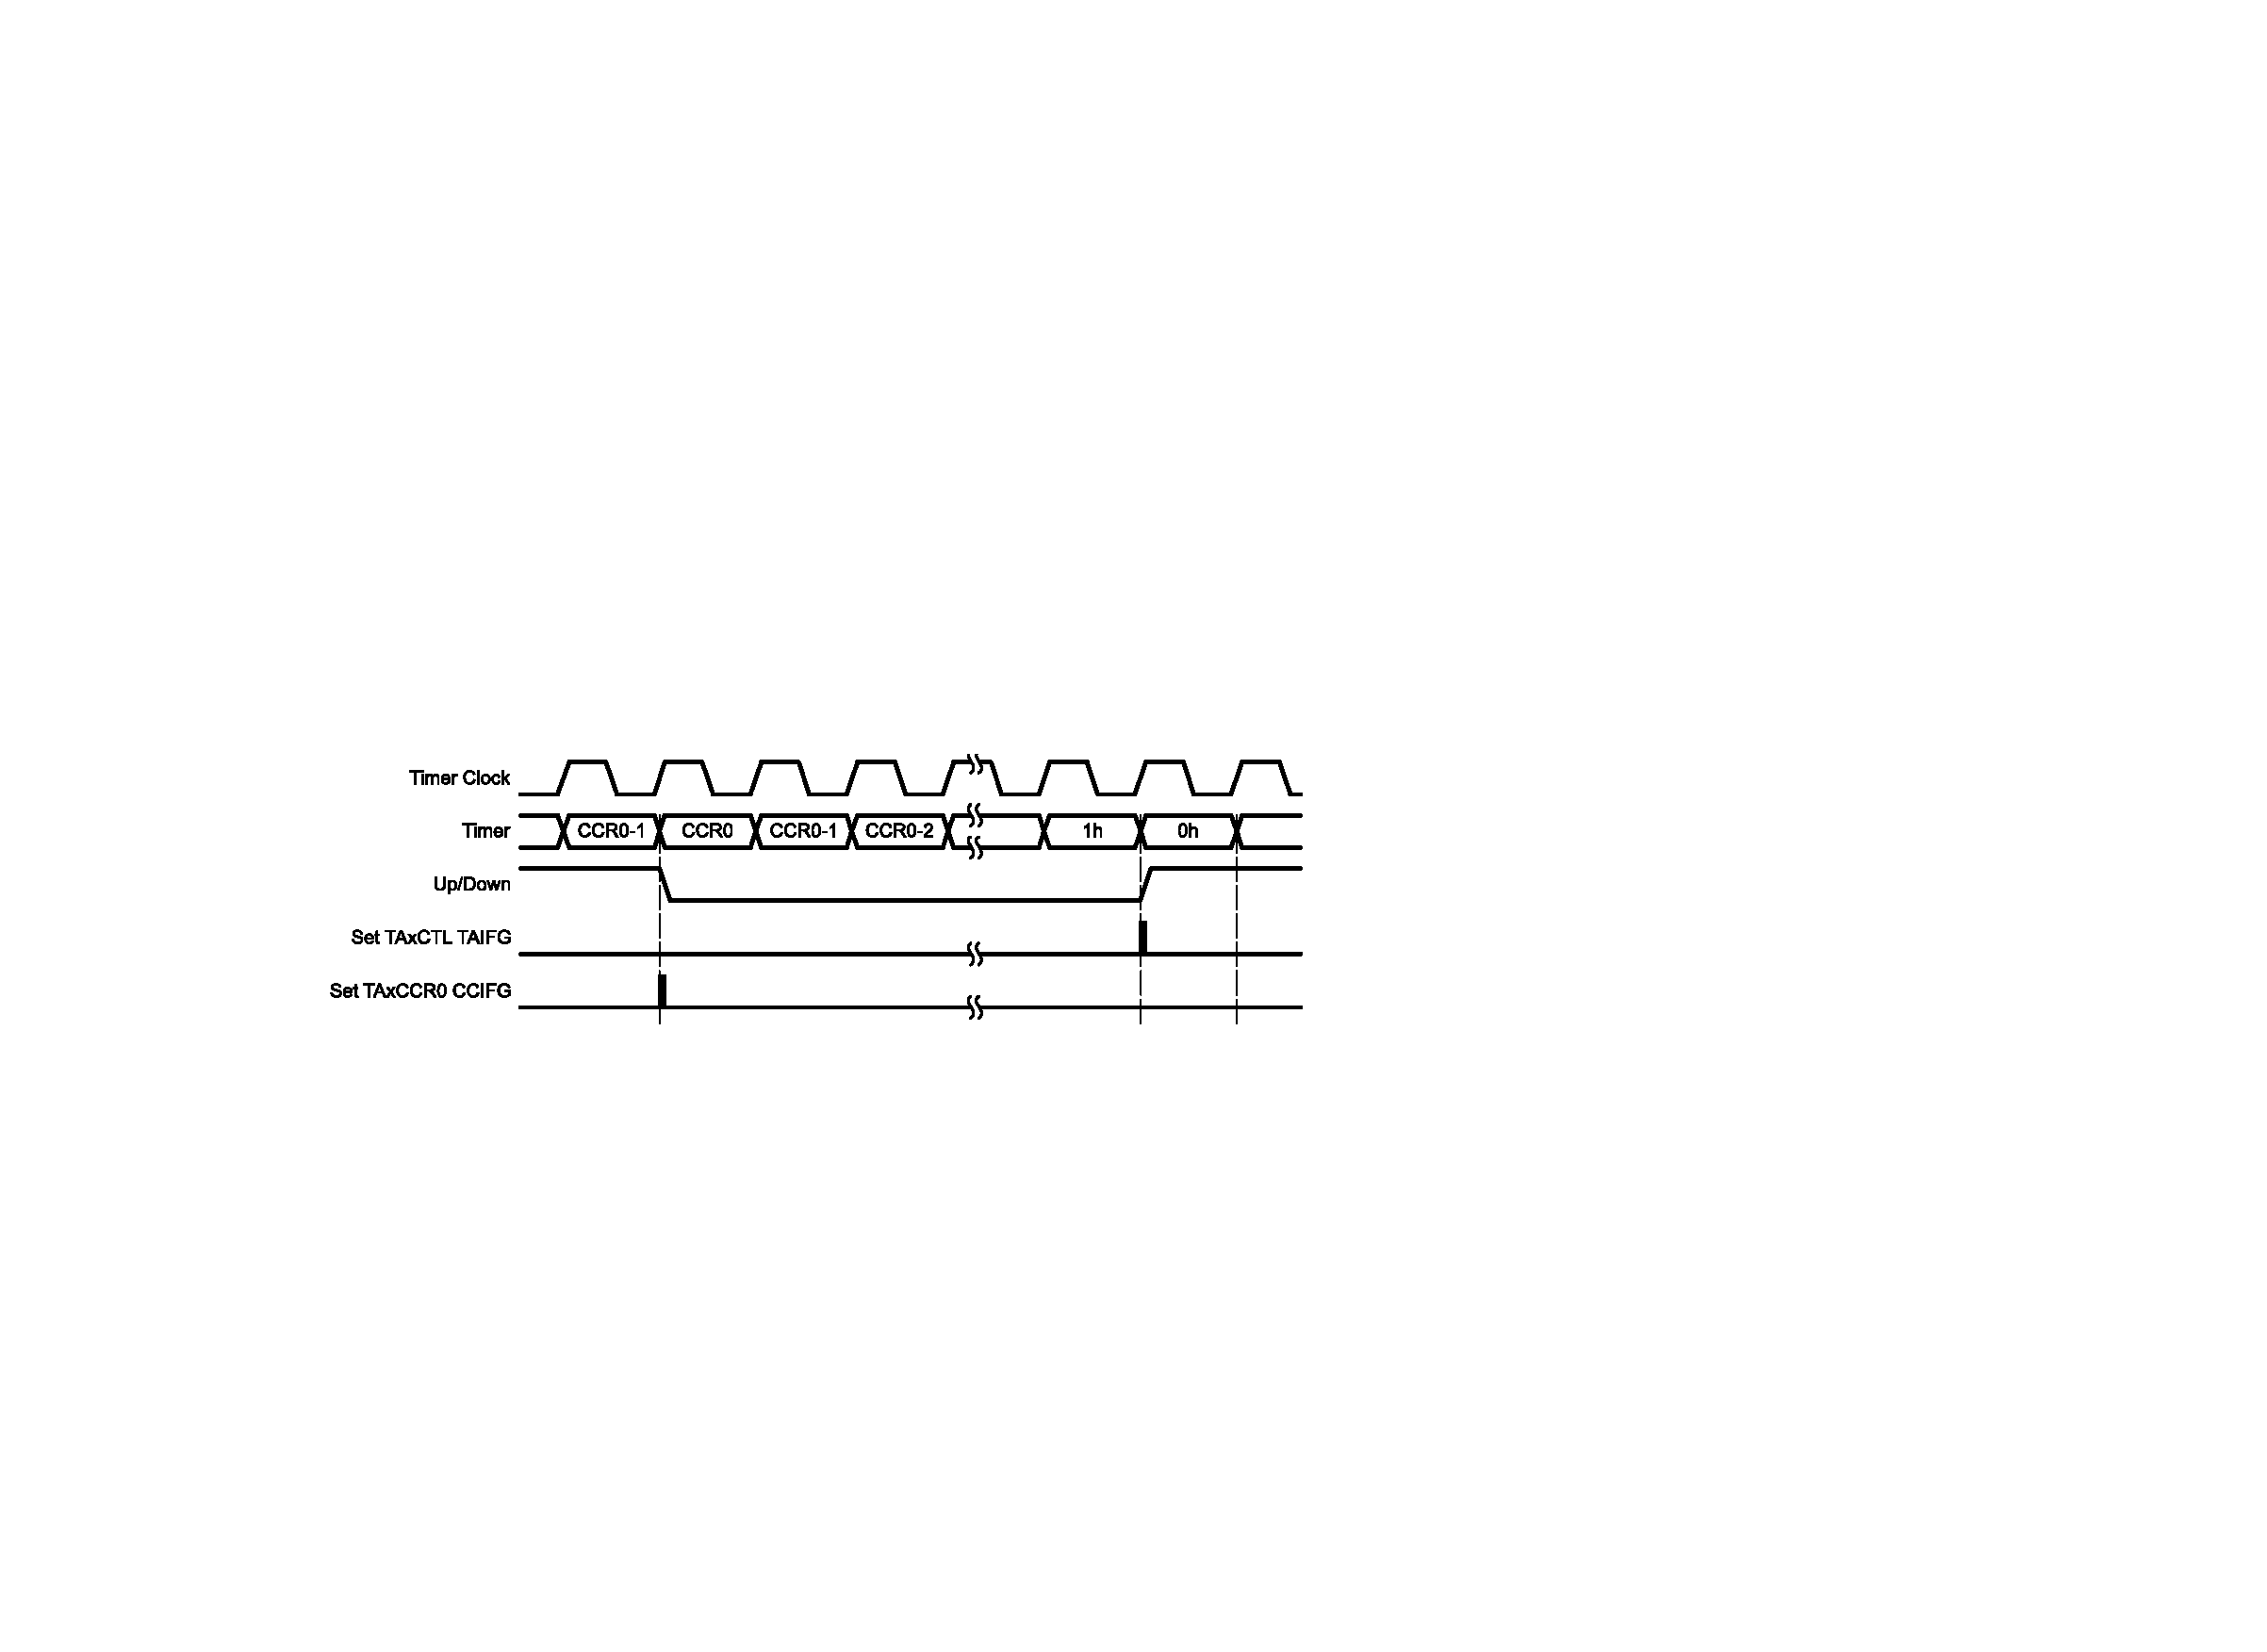
\includegraphics[angle=0, width=12cm]{./Figures/Chap5_Timer/Timer_Mode_3b.pdf}
  \rule{35em}{0.5pt}
  \caption[TimerA Mode 3]{Comptage en mode 3: d�tail des signaux CCIFG et TAIFG)}
  \label{fig:TimerAmode3b}
\end{figure}

Gr�ce � cette vari�t� des modes de comptage, le timer A va �tre capable de g�n�rer un grand nombre de signaux diff�rents.


\subsection{Structure d�taill�e du timer A}
La figure \ref{fig:TimerAstruct} illustre plus en d�tail la structure du timer A, en mettant en �vidence uniquement les registres et les signaux de sortie du timer. Comme dit pr�c�demment, il peut y avoir 3, 5 ou 7 blocs de "capture/comparaison". Sur la figure, n vaut donc 2, 4 ou 6.

\begin{figure}[htb]
  \centering
  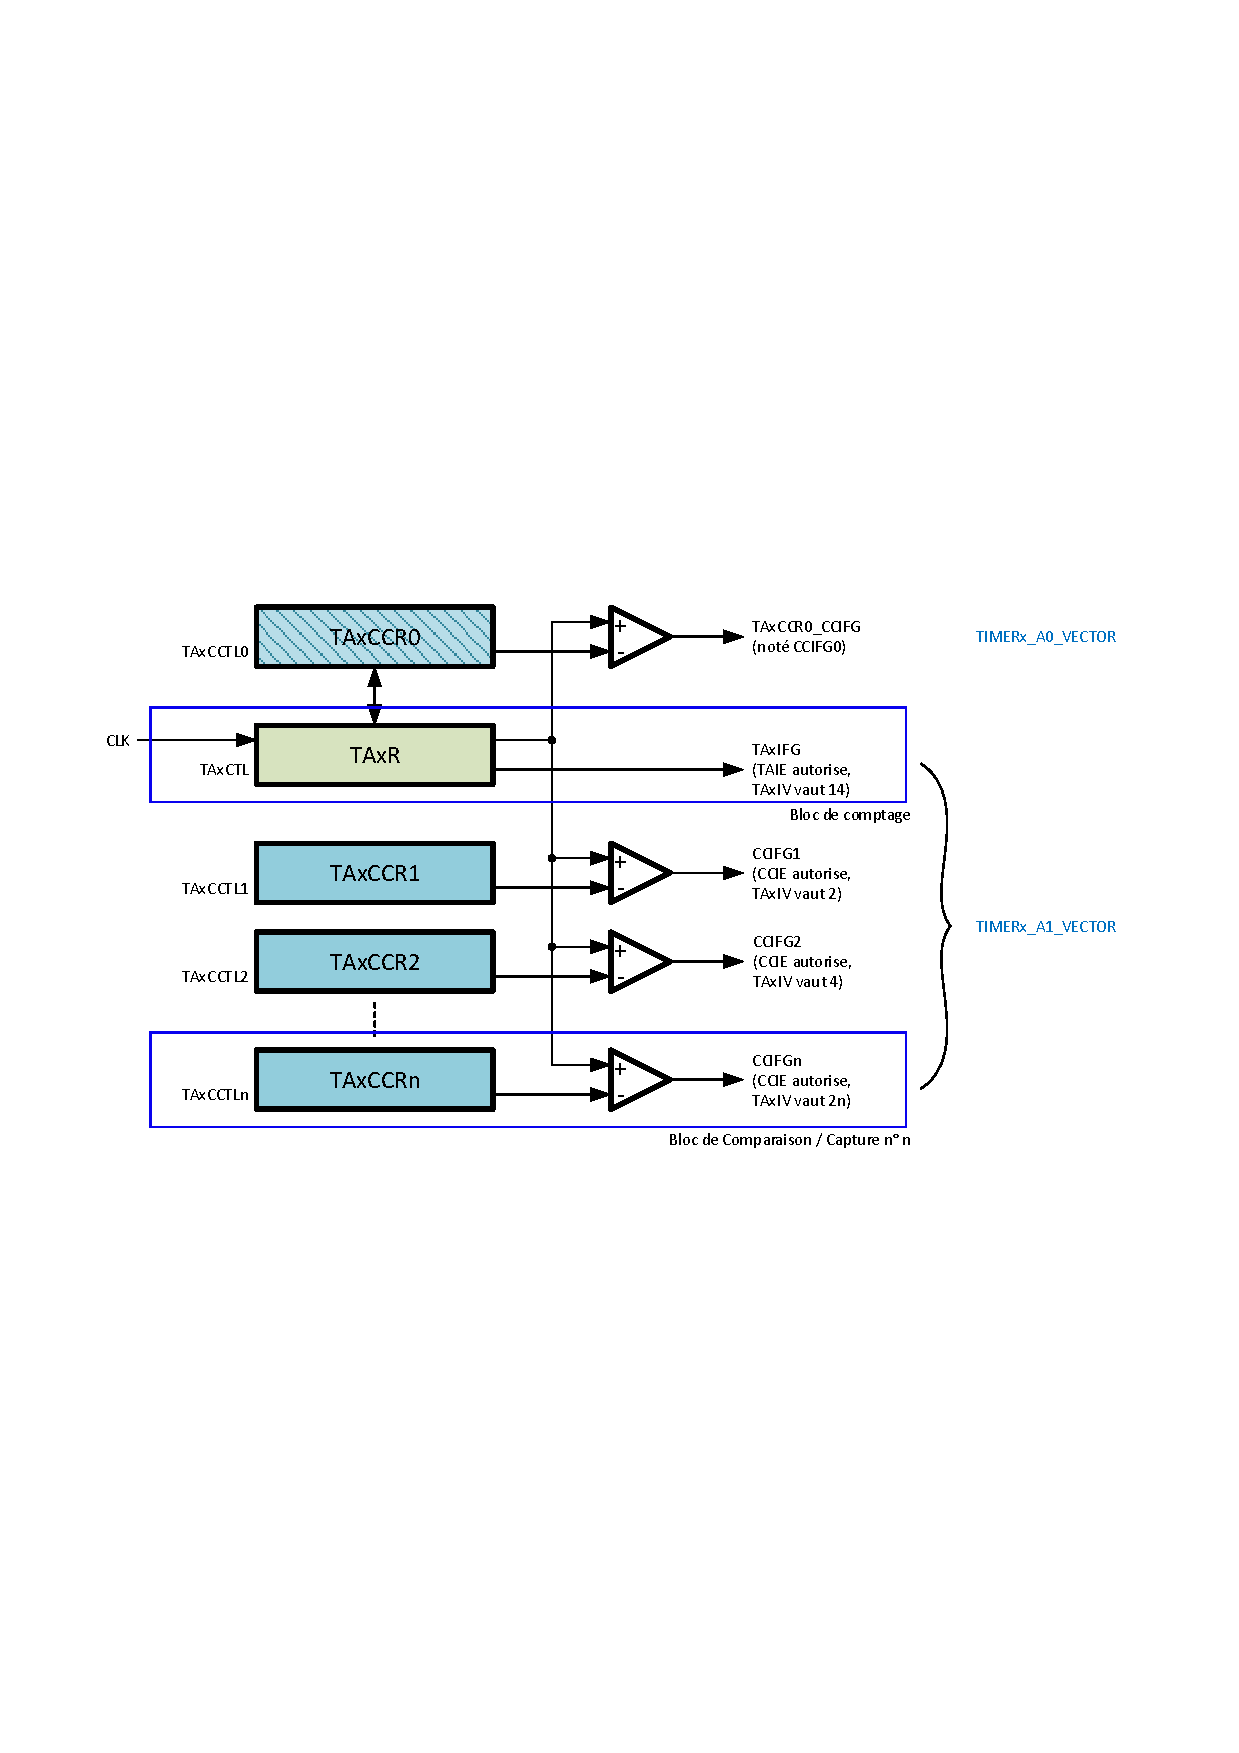
\includegraphics[angle=0, width=14cm]{./Figures/Chap5_Timer/Timer_blocs_2.pdf}
  \rule{35em}{0.5pt}
  \caption[Structure TimerA]{Organisation structurelle du timer A}
  \label{fig:TimerAstruct}
\end{figure}

Le timer est ainsi organis� en tranches, chacune capable de g�n�rer ses signaux propres. Dans la figure \ref{fig:TimerAstruct}, chaque rectangle repr�sente un �registre de donn�e�, c'est � dire un registre qui contient une information repr�sentant une grandeur.
Gr�ce � leur module de sortie, les circuits de capture/comparaison peuvent aussi g�n�rer automatiquement des signaux particuliers sur une patte du microcontr�leur. Ces fonctionnalit�s n'apparaissent pas sur la figure \ref{fig:TimerAstruct}.
A gauche de chaque �registre de donn�e� est not� le nom de son registre de contr�le. Par exemple, � gauche du registre TAxR on retrouve le nom de son registre de contr�le : TAxCTL (TAx ConTroL). Tous ces registres sont sur 16 bits.

\subsection{Contr�le du bloc de comptage}
TAxR : Timer A Register (n� x) ou registre de comptage du timer n� x. Sa valeur �volue entre 0 et 0xFFFF ou le contenu de TAxCCR0.

TAxCTL : Timer A Control (n� x) ou registre de contr�le du comptage du timer n� x. Il permet de sp�cifier le comportement du bloc de comptage.
Il est compos� de 5 champs, pour:
\begin{itemize}[label=\textbullet,font=\small]
\item s�lectionner l'horloge de r�f�rence (champ TASSEL)
\item s�lectionner le facteur de pr�division de l'horloge de r�f�rence (champ ID)
\item s�lectionner le mode de comptage (champ MC)
\item la remise � 0 (reset) du registre de comptage TAxR
\item l'autorisation des interruptions (TAIE) issues du registre de comptage. A l'�vidence, ces interruptions ne peuvent �tre g�n�r�es qu'au moment particulier o� le registre de comptage TAxR est � 0, puisqu'on ne connait pas la valeur maximale que peut prendre le registre de comptage TAxR.
\end{itemize}

Un dernier champ (TAIFG) contient le flag d'�tat de l'interruption issue du registre de comptage TAxR.
\\
La figure \ref{fig:TimerTAR} illustre en d�tail le bloc de comptage. On y voit les diff�rents sous blocs et leurs champs de contr�le, tous �l�ments du registre de contr�le TAxCTL.

\begin{figure}[htb]
  \centering
  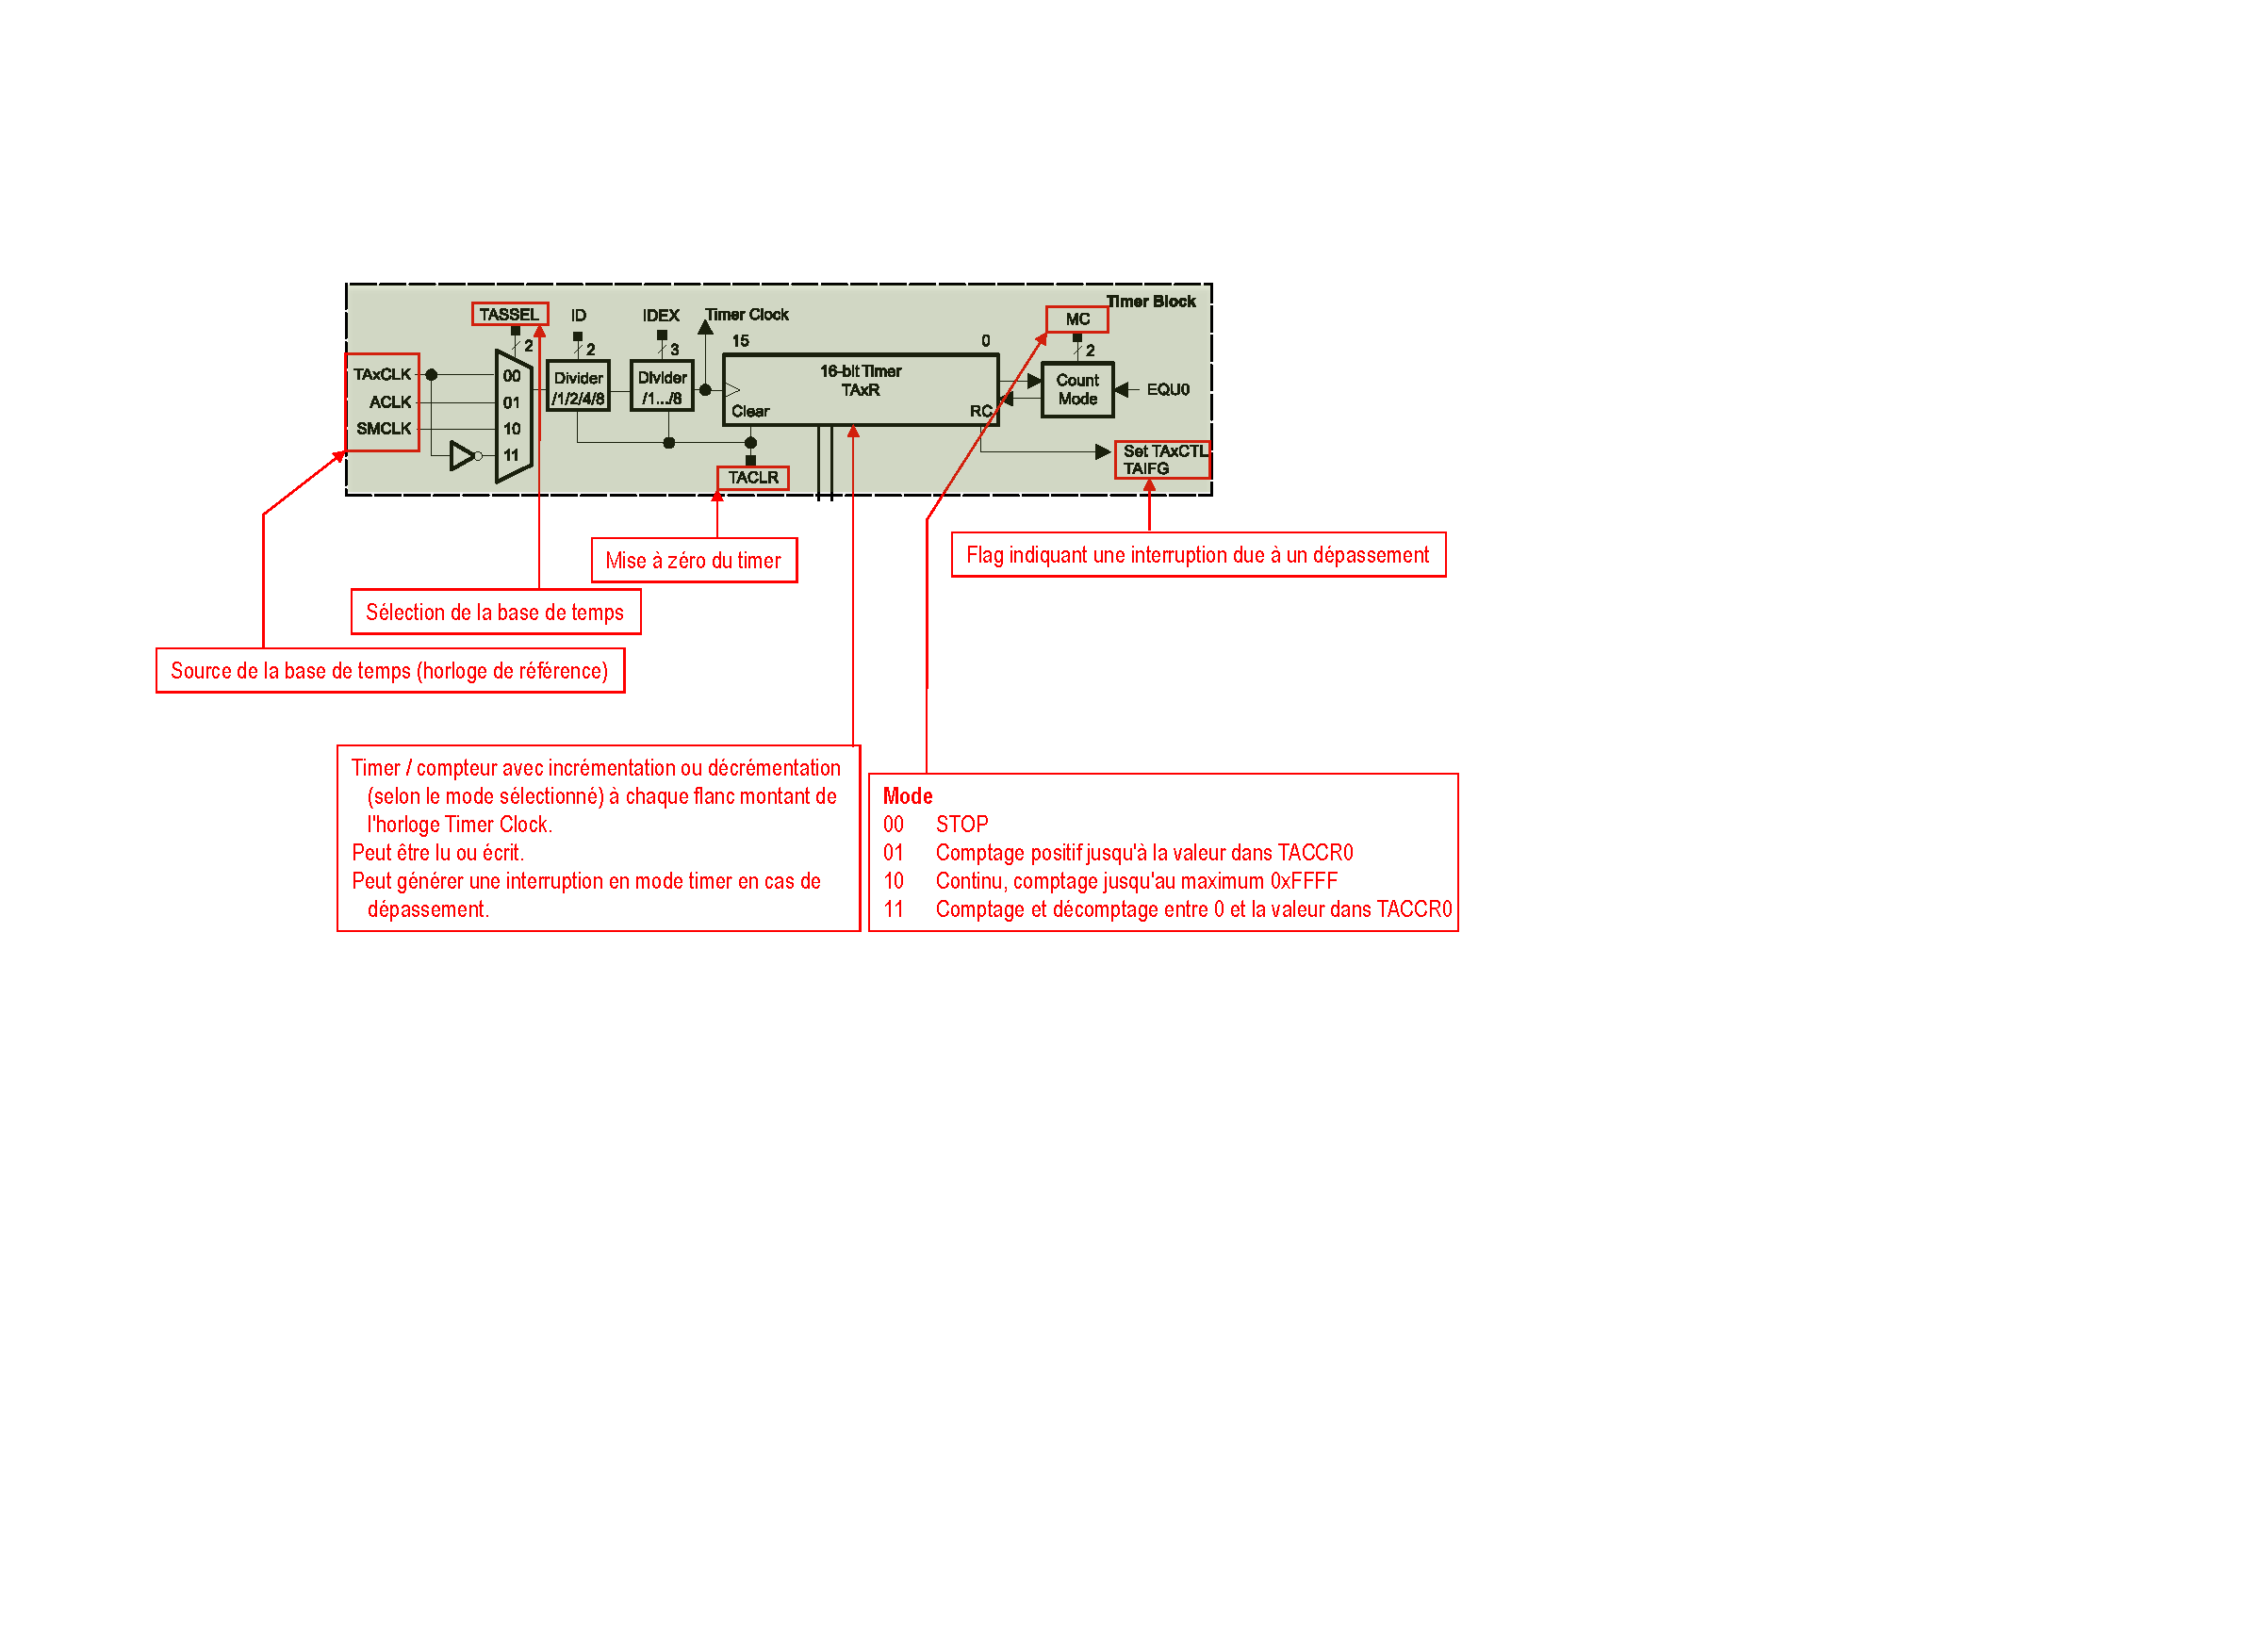
\includegraphics[angle=0, width=16cm]{./Figures/Chap5_Timer/Timer_Detail_1.pdf}
  \rule{35em}{0.5pt}
  \caption[TimerTAR]{Sch�ma de d�tail du bloc de comptage}
  \label{fig:TimerTAR}
\end{figure}

Le d�tail du registre de contr�le TAxCTL est donn� � la figure \ref{fig:TAxCTL} et dans le tableau \ref{table:TAxCTL}.

\begin{figure}[htb]
  \centering
  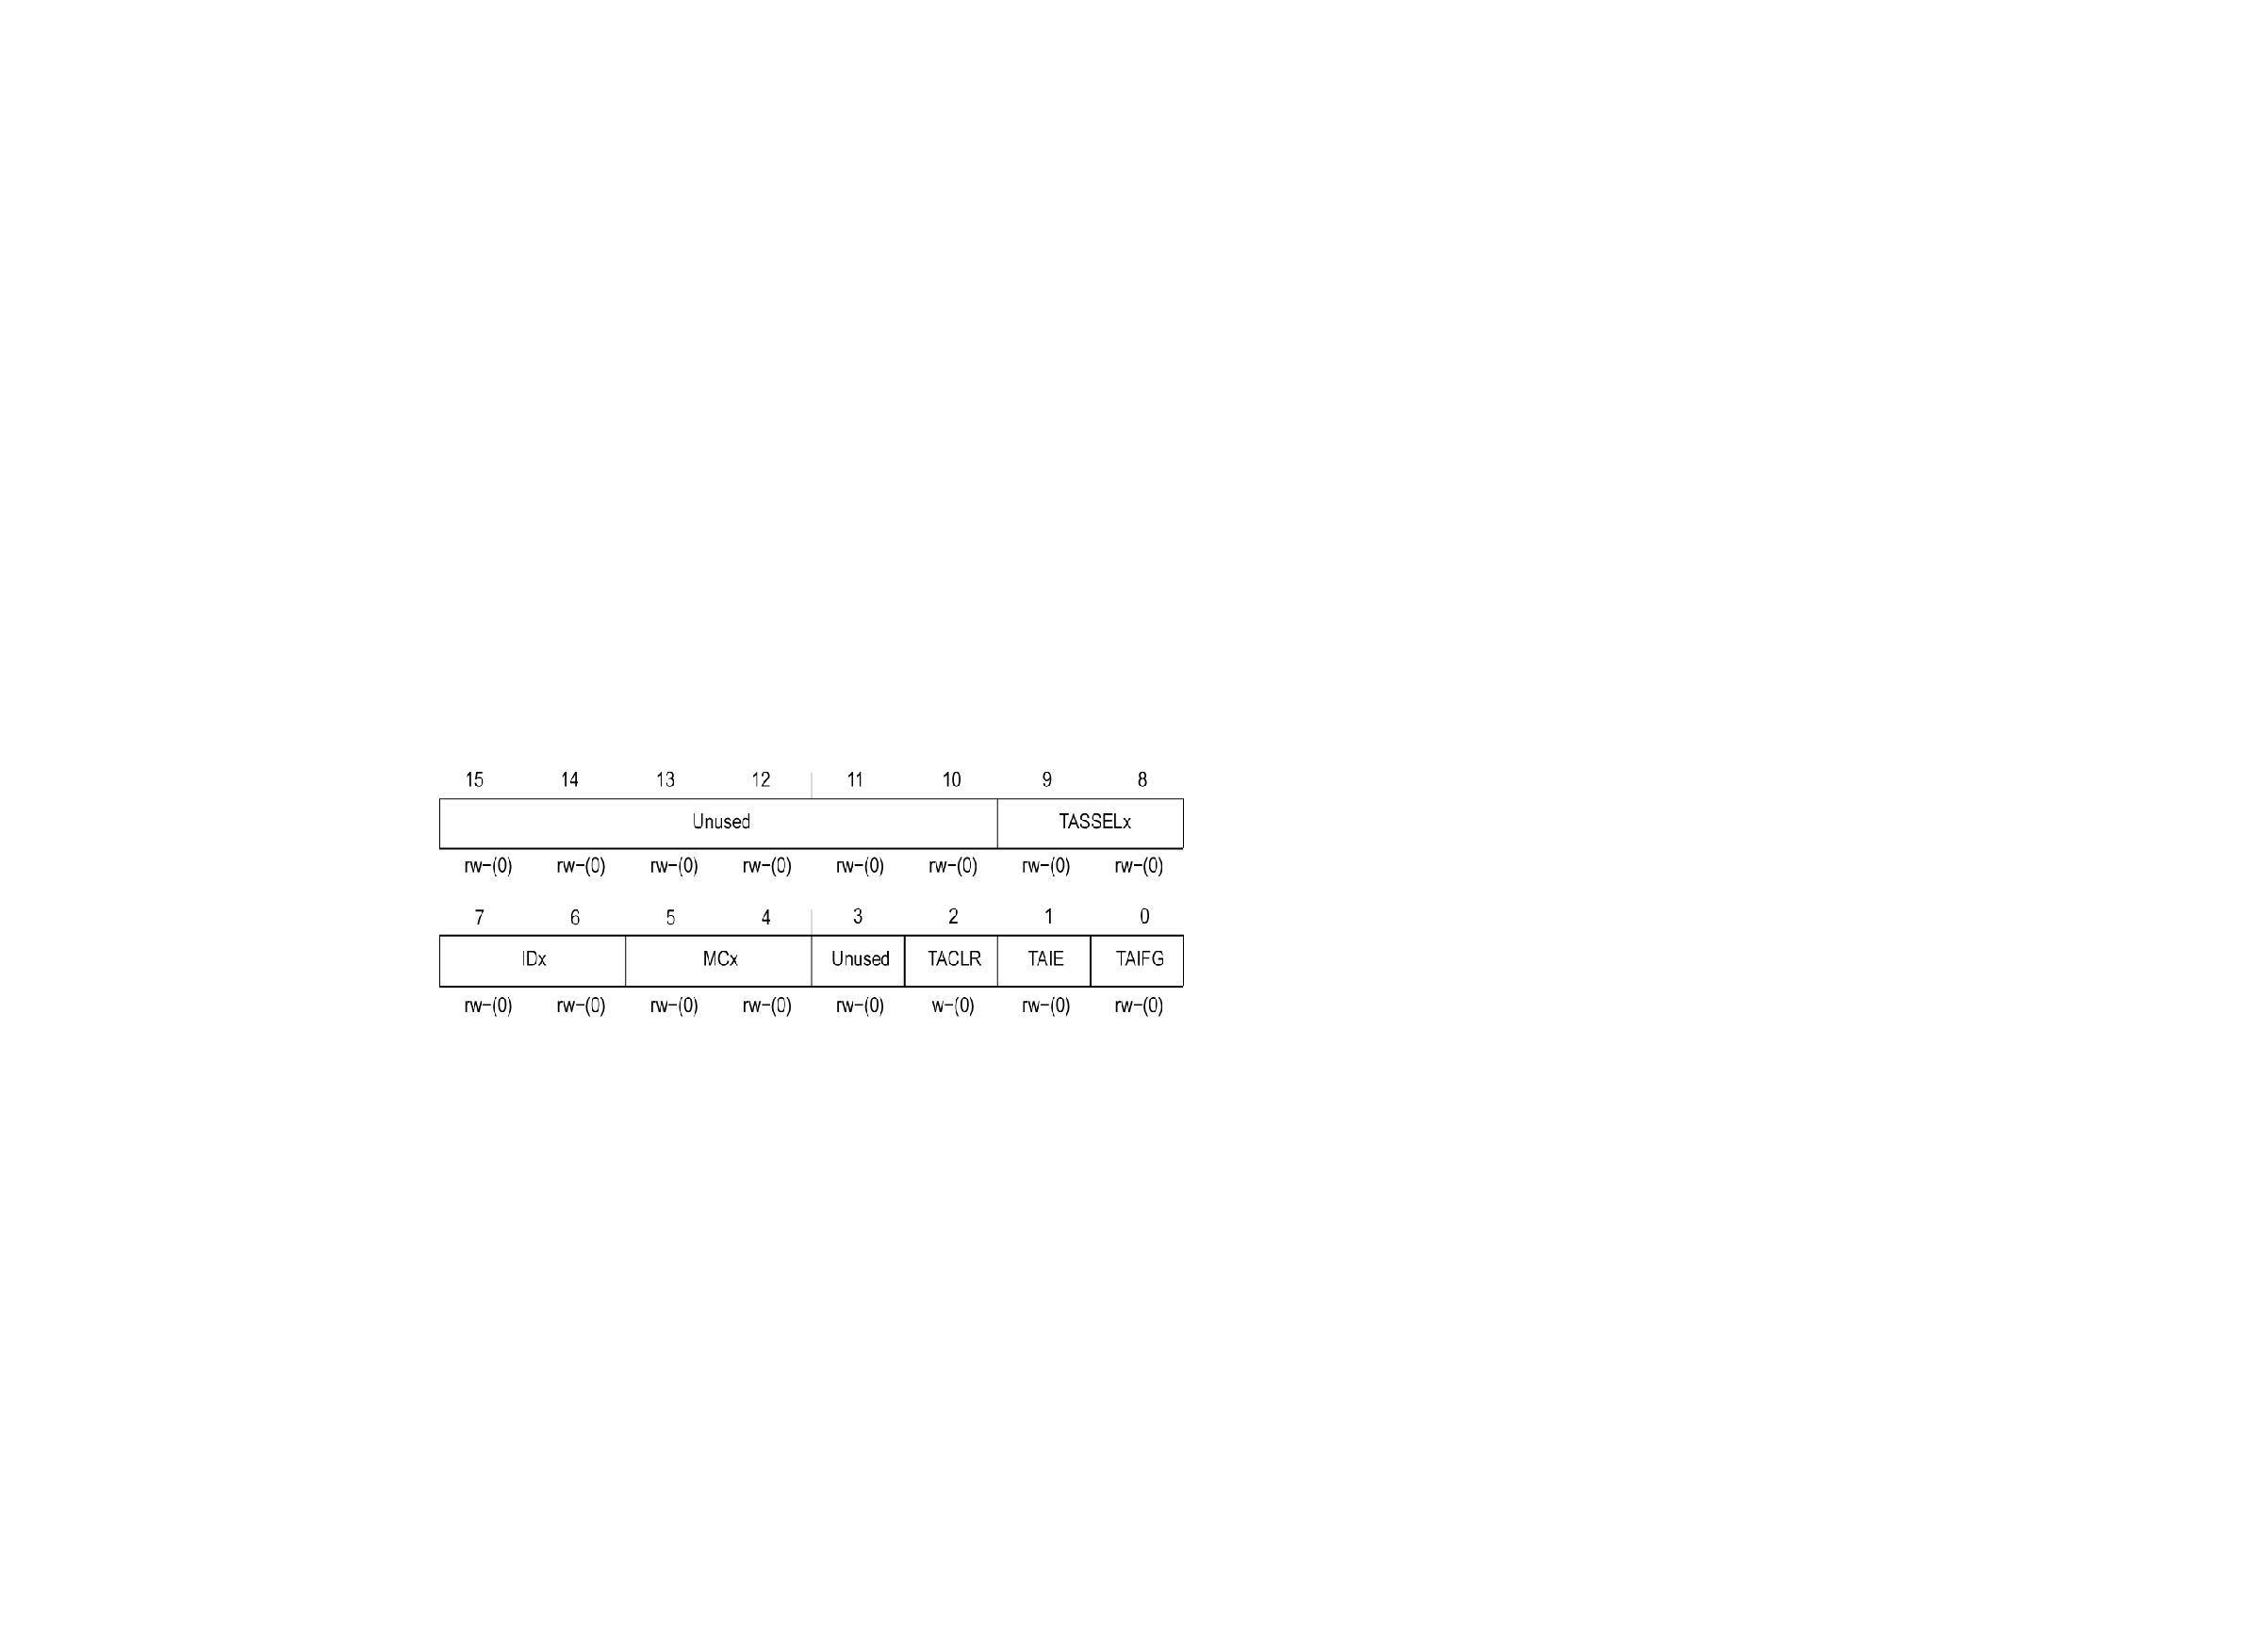
\includegraphics[angle=0, width=13cm]{./Figures/Chap5_Timer/TAxCTL.pdf}
  \rule{35em}{0.5pt}
  \caption[TAxCTL]{Registre TAxCTL}
  \label{fig:TAxCTL}
\end{figure}

\begin{table}[htb]
\centering 
\begin{tabular}{l l l l}
\hline\hline
Champ & & Valeur & Description \\ %[0.5ex]
\hline
TASSEL & & & S�lection de l'horloge d'incr�mentation  \\
& & 00 & TAxCLK  \\
& & 01 & ACLK  \\
& & 10 & SMCLK  \\
& & 11 & INCLK  \\
\hline
ID & & & Pr�division de l'horloge d'incr�mentation  \\
& & 00 & /1  \\
& & 01 & /2  \\
& & 10 & /4  \\
& & 11 & /8  \\
\hline
MC & & & Mode de comptage  \\
& & 00 & Stop. Le timer est arr�t�  \\
& & 01 & Mode Up. Le timer compte jusqu'� TAxCCR0  \\
& & 10 & Mode continu. Le timer compte jusqu'� 0xFFFF  \\
& & 11 & Mode Up/Down. Le timer compte jusqu'� TAxCCR0 puis d�compte jusqu'� 0  \\
\hline
TACLR & & & Met TAxR � 0. TACLR revient automatiquement � 0 \\
\hline
TAIE & & & Autorisation des requ�tes d'interruptions de TAIFG \\
& & 0 & Interruptions non autoris�es \\
& & 1 & Interruptions autoris�es \\
\hline
TAIFG & & & Indicateur d'interruption \\
& & 0 & Aucune interruption n'est en attente \\
& & 1 & Une interruption est en attente de traitement \\
\hline
\end{tabular}
\caption{Description des champs du registre TAxCTL}
\label{table:TAxCTL}
\end{table}

\begin{minipage}{14cm}{
\subsubsection*{Exemple de configuration}
Les instructions ci-dessous configurent le timer A0 en mode comptage de 0 (inclus) jusqu'� 8191 (inclus), avec l'horloge SMCLK pr�divis�e par 8.
{\fontfamily{pcr}\selectfont
\begin{tabbing}
\qquad    \= \#define TASSEL\_2	\= (2*0x100u) \\
\qquad \> \#define ID\_3       \> (3*0x40u) \\
\qquad \> \#define MC\_1       \> (1*0x10u) \\
\\
\qquad \> TA0CCR0 = 8191; \\
\qquad \> TA0CTL  = TASSEL\_2 | MC\_1 | ID\_3; \\
\end{tabbing}
}
}
\end{minipage}


\subsection{Contr�le du bloc de capture/comparaison n�0}
Ce bloc fonctionnel est en �troite interaction avec le registre de comptage TAxR, puisqu'il peut (selon la valeur du champ MC) d�finir la borne sup�rieure du comptage.

TAxCCR0 : registre de capture/comparaison n� 0 pour le Timer A (n� x). Comme TAxR, TAxCCR0 est un � registre de donn�e �; leurs valeurs peuvent �tre compar�es (mode comparaison) ou le contenu de TAxR peut �tre copi� dans TAxCCR0 (mode capture).
Lors de ces deux �v�nements (�galit� des deux registres ou transfert de TAxR dans TAxCCR0), une requ�te d'interruption est �mise; c'est le signal appel� TAxCCR0\_CCIFG, que nous nommerons CCIFG0.
Ce circuit de capture/compare, centr� autour du registre TAxCCR0, est contr�l� par le registre de contr�le TAxCCTL0.

TAxCCTL0 : registre de contr�le du circuit de capture/compare n� 0 pour le Timer A (n� x). Il permet de sp�cifier comment TAxCCR0 se comporte. Il est compos� de 6 champs, pour:
\begin{itemize}[label=\textbullet,font=\small]
\item s�lectionner la fonction Capture ou Comparaison (CAP)
\item s�lectionner le mode de capture (sur flanc montant, descendant, etc...) (CM)
\item s�lectionner le signal de capture (CCIS)
\item synchroniser ou non du signal de capture avec l'horloge de comptage (SCS)
\item s�lectionner le mode de sortie (OUTMOD)
\item autoriser ou non les interruptions �mises par le bloc de capture comparaison n� 0 (CCIE)
\end{itemize}

D'autres champs contiennent diff�rents signaux tels que le flag de l'interruption issue du bloc (CCIFG0).
\\
La figure \ref{fig:TimerCCR} illustre en d�tail un bloc de capture/comparaison (n� y). On y voit les diff�rents sous blocs et leurs champs de contr�le, tous �l�ments du registre de contr�le TAxCCTLy.

\begin{figure}[htb]
  \centering
  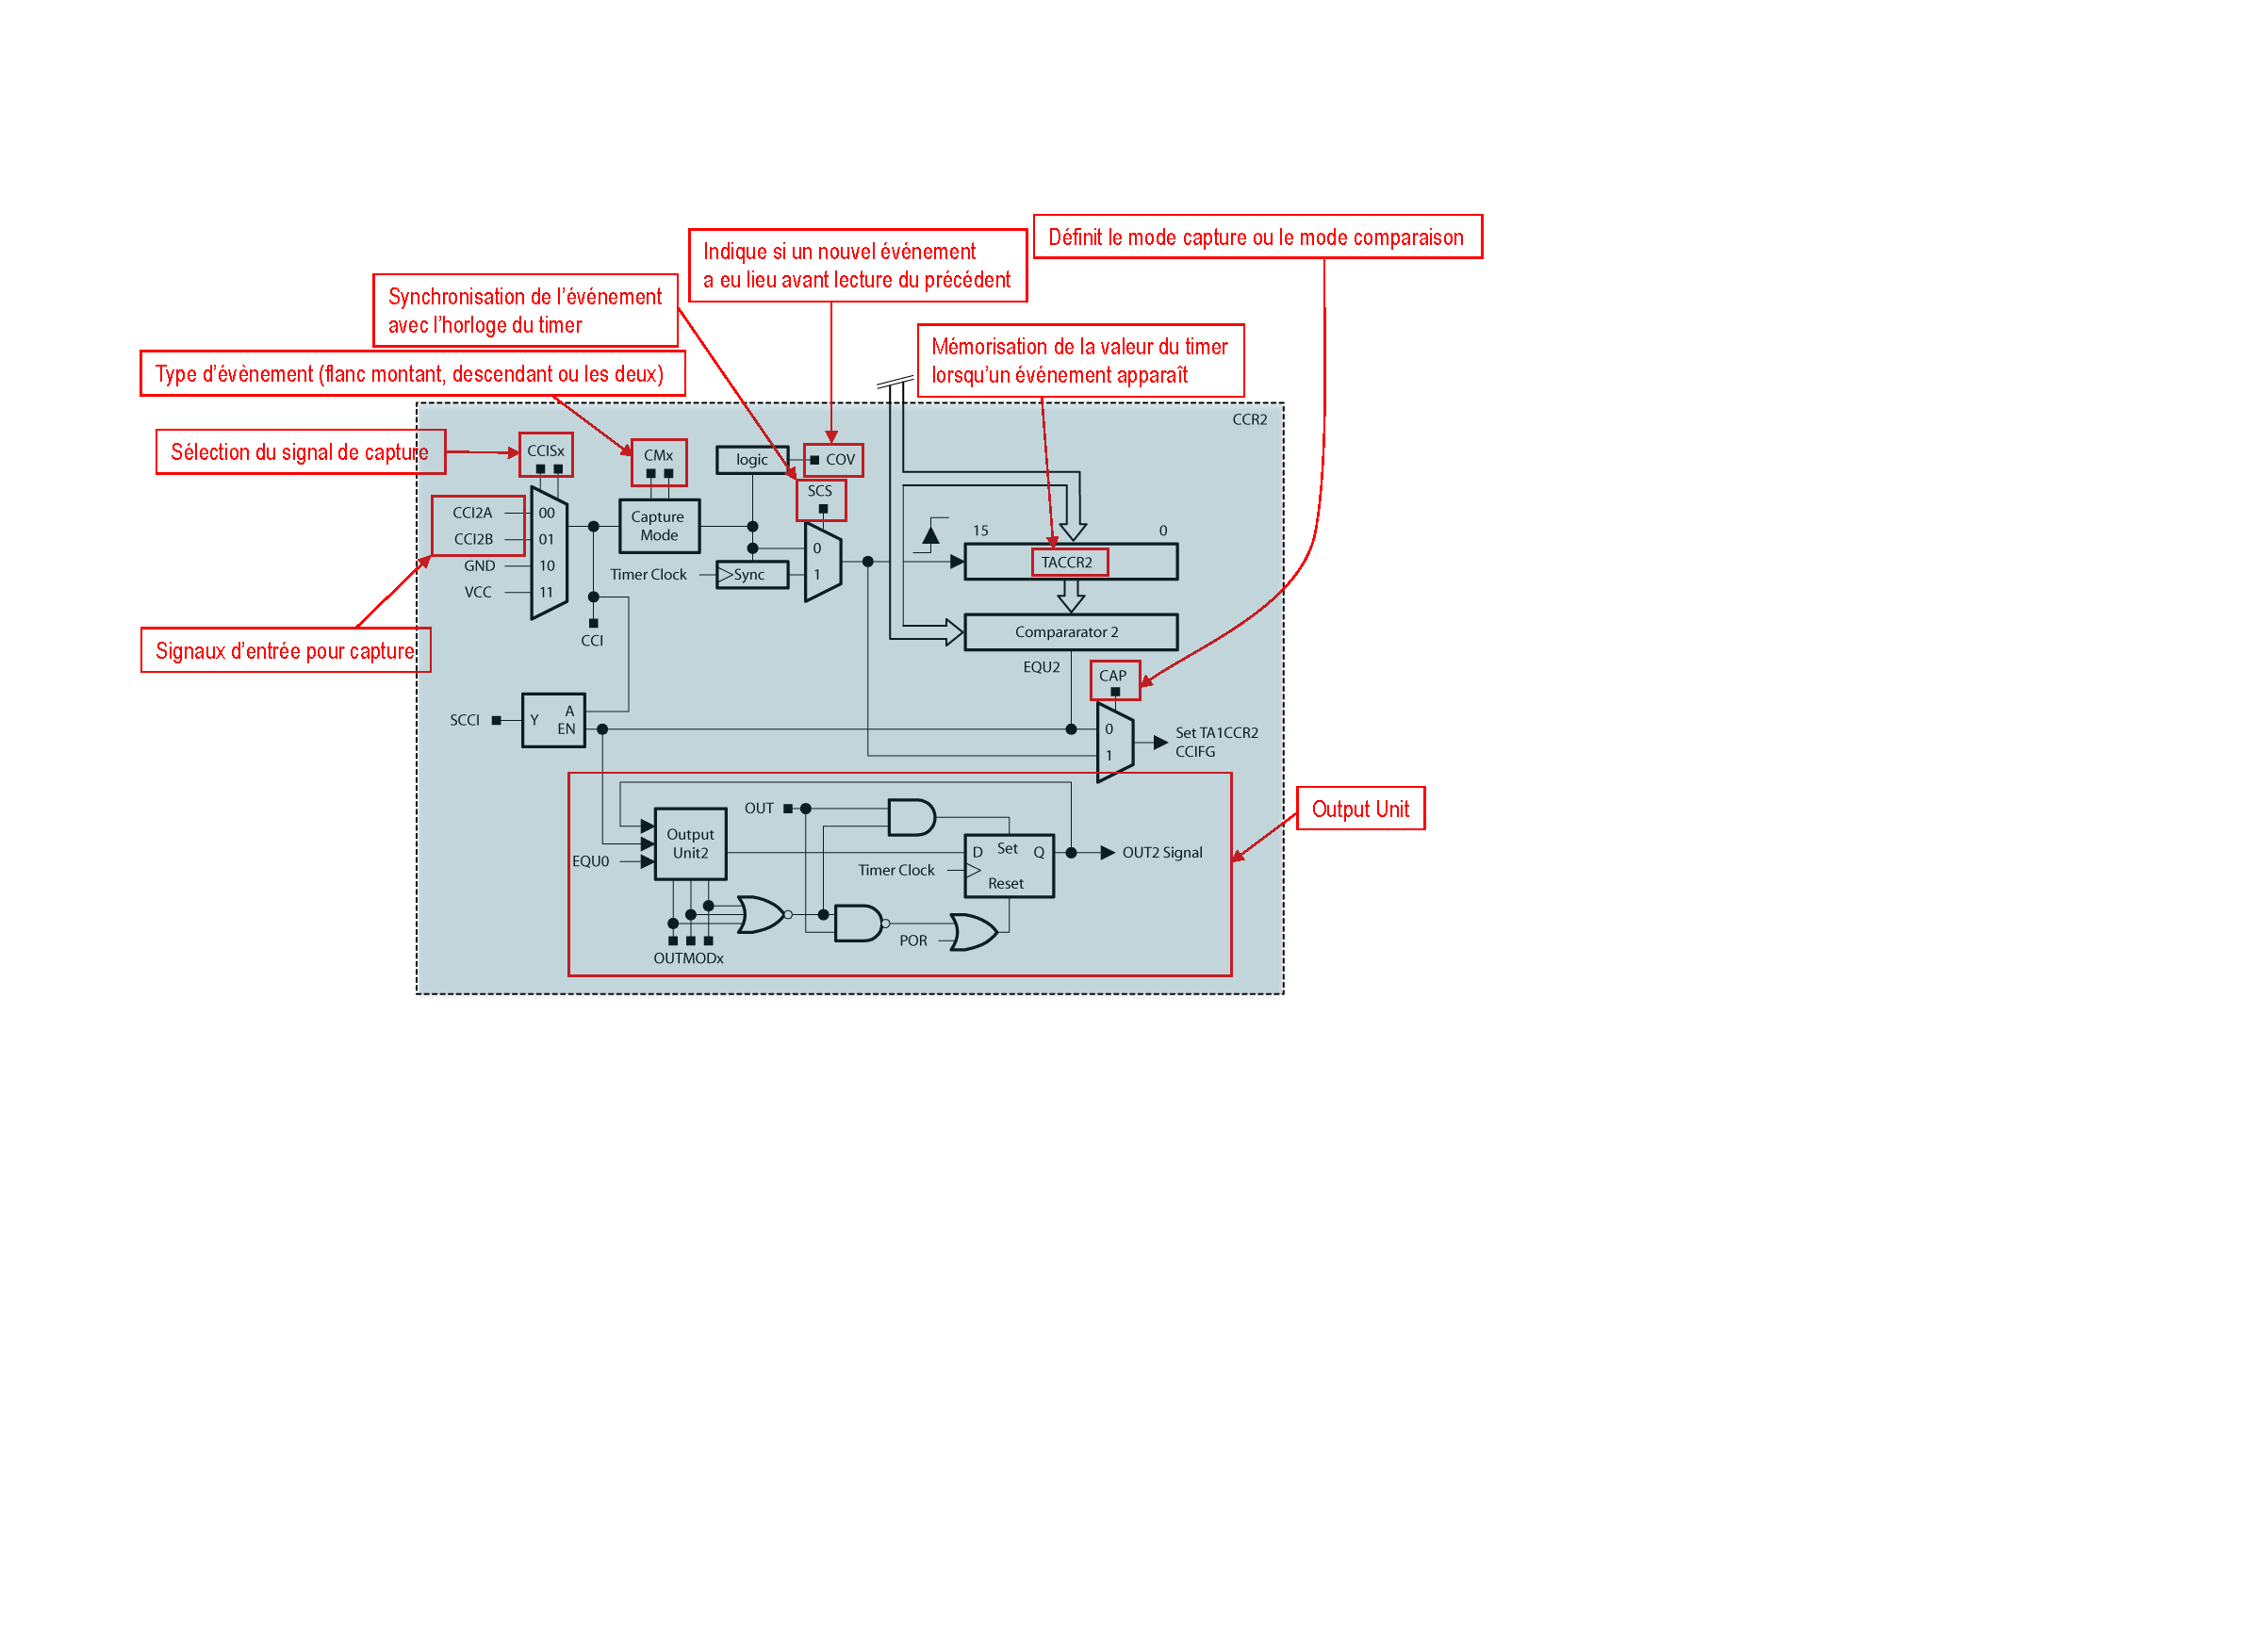
\includegraphics[angle=0, width=16cm]{./Figures/Chap5_Timer/Timer_Detail_2.pdf}
  \rule{35em}{0.5pt}
  \caption[TimerCCR]{Sch�ma de d�tail du bloc de capture/comparaison}
  \label{fig:TimerCCR}
\end{figure}

Le d�tail du registre de contr�le TAxCCTLy, pour le bloc de capture/comparaison n�y, est donn� � la figure \ref{fig:TAxCCTLy} et dans le tableau \ref{table:TAxCCTL}. 

\begin{figure}[htb]
  \centering
  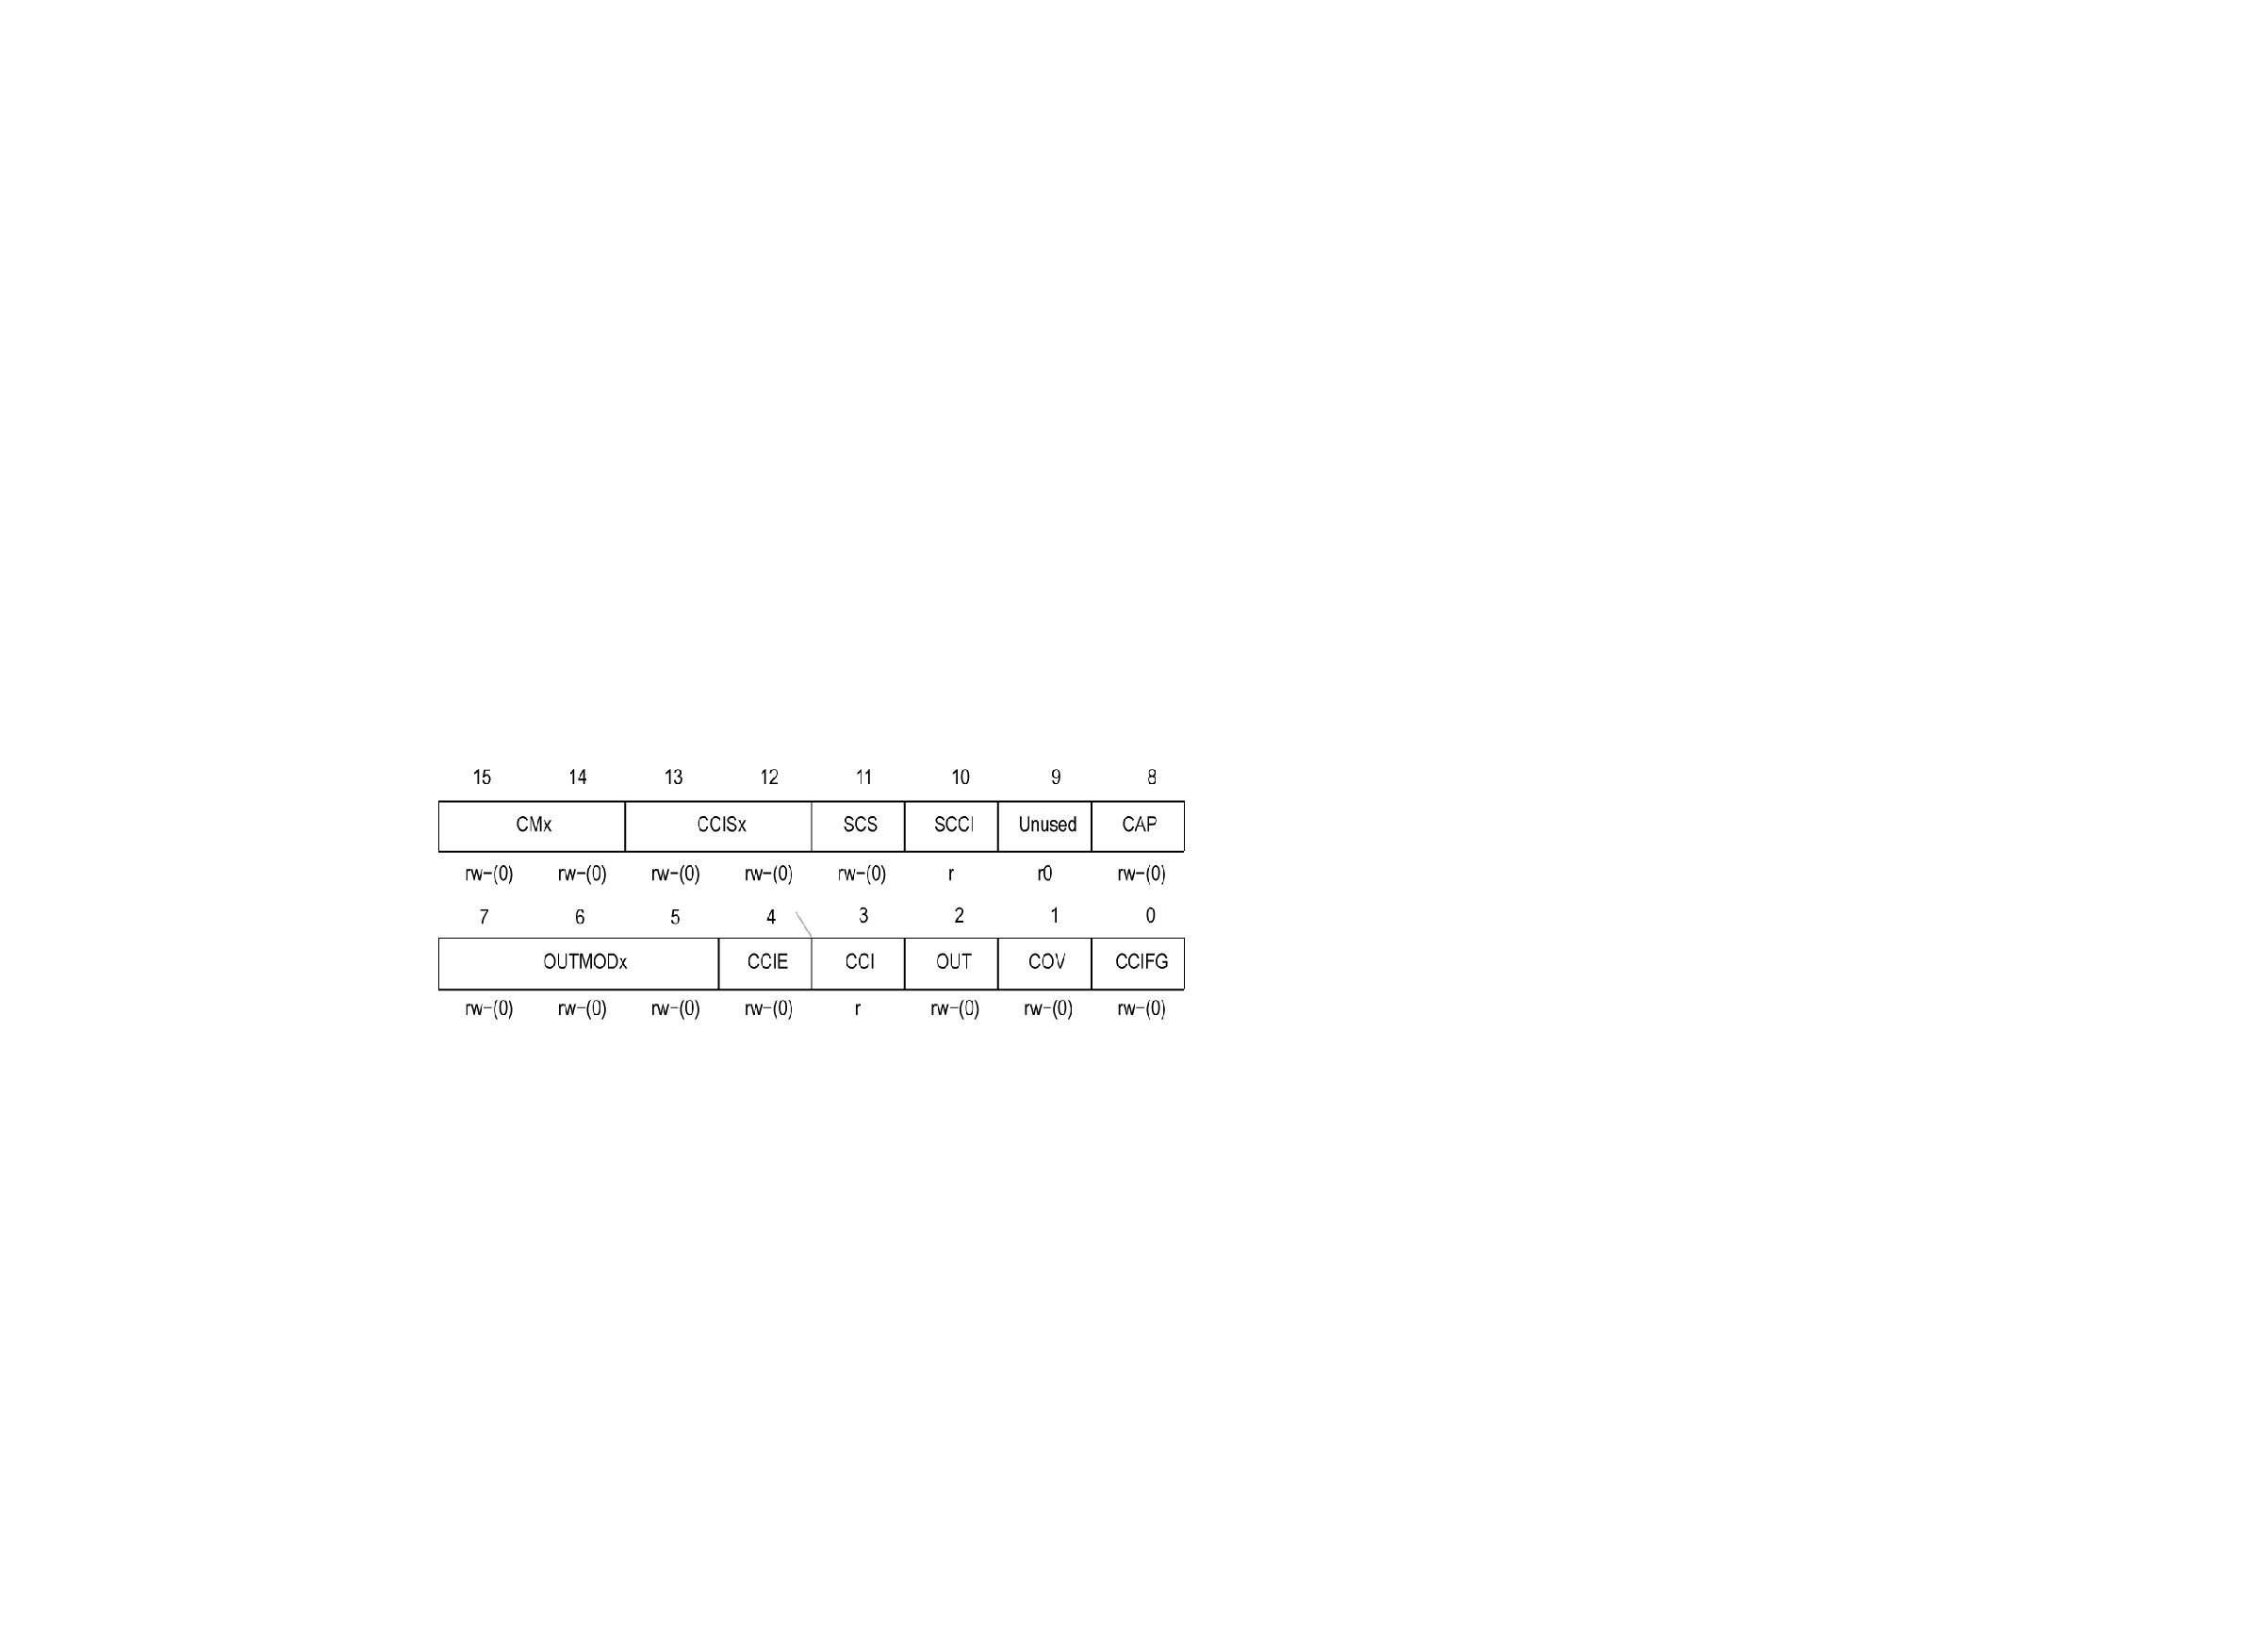
\includegraphics[angle=0, width=13cm]{./Figures/Chap5_Timer/TAxCCTLy.pdf}
  \rule{35em}{0.5pt}
  \caption[TAxCCTLy]{Registre TAxCCTLy}
  \label{fig:TAxCCTLy}
\end{figure}

\begin{table}[htb]
\centering 
\begin{tabular}{l l l l}
\hline\hline
Champ & & Valeur & Description \\ %[0.5ex]
\hline
CM & & & Mode de capture  \\
& & 00 & Pas de capture  \\
& & 01 & Capture sur le flanc montant du signal de capture  \\
& & 10 & Capture sur le flanc descendant  \\
& & 11 & Capture sur les deux flancs  \\
\hline
CCIS & & & S�lection du signal de capture  \\
& & 00 & CCIxA  \\
& & 01 & CCIxB  \\
& & 10 & GND  \\
& & 11 & VCC  \\
\hline
SCS & & & Synchronisation du signal de capture  \\
& & 0 & Pas de synchronisation \\
& & 1 & Synchronisation du signal de capture avec le prochain flanc de CLK \\
\hline
SCCI & & & Image du signal de capture apr�s synchronisation \\
\hline
CAP & & & S�lection entre capture et comparaison \\
& & 0 & Mode comparaison \\
& & 1 & Mode capture \\
\hline
OUTMOD & & & G�n�ration du signal de sortie OUT (module de sortie) \\
& & 000 &  voir chapitre \ref{Module de sortie} \\ 
& & 001 &  \\
& & 010 &  \\
& & 011 &  \\
& & 100 &  \\
& & 101 &  \\
& & 110 &  \\
& & 111 &  \\
\hline
CCIE & & & Autorisation des requ�tes d'interruptions de CCIFG \\
& & 0 & Interruptions non autoris�es \\
& & 1 & Interruptions autoris�es \\
\hline
\end{tabular}
\caption{Description des champs du registre TAxCCTL}
\label{table:TAxCCTL}
\end{table}

\begin{minipage}{14cm}{
\subsubsection*{Exemple de configuration}
Les instructions ci-dessous reprennent la configuration vue au chapitre pr�c�dent, en autorisant de plus le bloc de capture/comparaison du timer A0 � �mettre des requ�tes d'interruptions par son signal CCIFG0.
{\fontfamily{pcr}\selectfont
\begin{tabbing}
\qquad    \= \#define TASSEL\_2	\= (2*0x100u) \\
\qquad \> \#define ID\_3       \> (3*0x40u) \\
\qquad \> \#define MC\_1       \> (1*0x10u) \\
\qquad \> \#define CCIE       \> (1*0x10u) \\
\\
\qquad \> TA0CCR0 = 8191; \\
\qquad \> TA0CTL  = TASSEL\_2 | MC\_1 | ID\_3; \\
\qquad \> TA0CCTL0  = CCIE; \\
\end{tabbing}
}
}
\end{minipage}

\subsection{Contr�le du bloc de capture/comparaison n�1,2,3...}
Ces circuits sont des copies conformes du circuit de capture/comparaison n� 0. La seule diff�rence est que leur coeur (TAxCCRy) n'a pas d'influence sur la borne sup�rieure de TAxR. Ils int�ragissent toutefois avec TAxR en mode capture.
Pour le circuit n� y, le registre de donn�e est nomm� TAxCCRy, le registre de contr�le est TAxCCTLy.
Bien entendu, dans le registre de contr�le TAxCCTLy, les champs portent les m�me noms (CAP, CM, CCIS, SCS, etc...).

\subsection{Diff�rence entre Capture et Comparaison}
La figure \ref{fig:CapvsComp} illustre le comportement du registre TAxR dans le mode 1 (continuous).

\begin{figure}[htb]
  \centering
  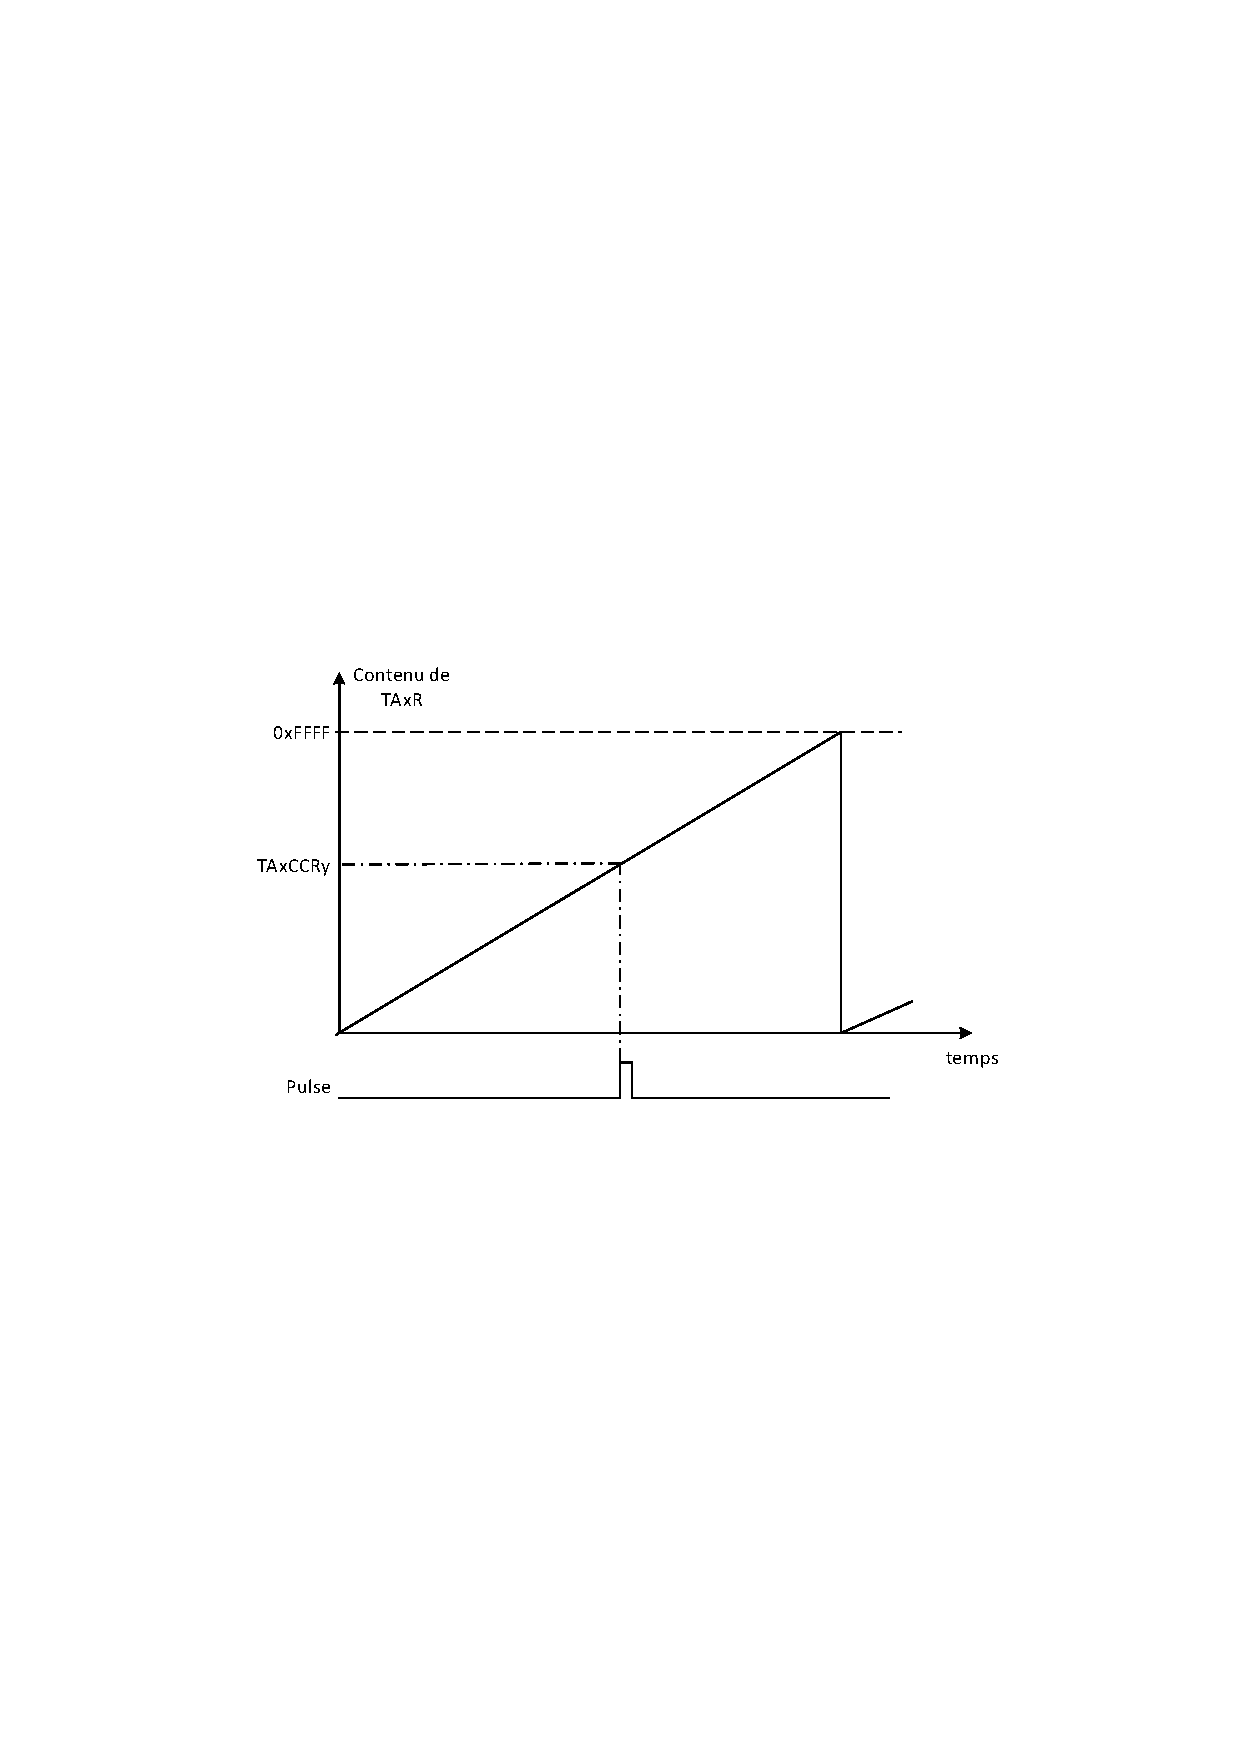
\includegraphics[angle=0, width=14cm]{./Figures/Chap5_Timer/Timer_CC.pdf}
  \rule{35em}{0.5pt}
  \caption[CapvsComp]{Comparaison : TAxR est l'entr�e / Capture : Pulse est l'entr�e}
  \label{fig:CapvsComp}
\end{figure}

Une fois le processus de comptage lanc�, TAxR �volue en dent de scie, comme illustr�. Le circuit de capture/comparaison utilise ce signal pour son op�ration.

En mode � comparaison �, le contenu du registre TAxCCRy est une entr�e. D�s que TAxR atteint TAxCCRy, le signal not� � Pulse � est g�n�r�, qui peut d�clencher l'ex�cution d'une routine de service d'interruption.

En mode � capture �, le contenu du registre TAxCCRy est une sortie. Un signal � Pulse � doit �tre fourni, qui d�clenche la copie de TAxR dans TAxCCRy au moment o� la pulse appara�t. En fait, c'est le flanc actif de la pulse qui d�clenche le processus de capture, qui peut donc se produire sur le flanc montant, descendant ou les deux, du signal � pulse �. Typiquement, le signal � pulse � est une entr�e du microcontr�leur. Au moment o� la capture est ex�cut�e, une requ�te d'interruption peut �tre �mise.

\subsection{Interruptions du timer A}
Un timer A contenant n bloc de capture/comparaison peut g�n�rer $n+1$ requ�tes d'interruptions. Toutefois, seuls deux vecteurs d'interruption sont d�finis. 
Revenant � la figure \ref{fig:TimerAstruct}, on voit que le signal CCIFG0 issu du bloc de capture/comparaison n�0 est associ� � lui tout seul � un des vecteurs (TIMERx\_A0\_VECTOR). Tous les autres signaux d'interruption (TAxIFG, CCIFG1, CCIFG2, ...) sont associ�s � l'autre vecteur (TIMERx\_A1\_VECTOR).

Si une interruption provient d'un des signaux TAIFG, CCIFG1 ou CCIFG2, il est donc n�cessaire de tester lequel de ces signaux est effectivement responsable de la requ�te. L'information y relative est disponible dans registre particulier TAIV, appel� abusivement "vecteur d'interruption". Il est ainsi possible de d�terminer rapidement la source de l'interruption, en testant la valeur de TAIV au moyen d'une instruction \textit{SWITCH...CASE}.

%\begin{minipage}{20cm}{
La description du registre TAIV est donn�e ci-dessous :
\begin{table}[htb]
\centering 
\begin{tabular}{l l l}
\hline\hline
Champ & Valeur & Source de l'interruption \\ %[0.5ex]
\hline                  % inserts single horizontal line
TAIV & 0x00 & pas d'interruption en attente  \\	% inserting body of the table
& 0x02 & CCIFG1  \\
& 0x04 & CCIFG2  \\
& 0x06 & CCIFG3  \\
& 0x08 & CCIFG4  \\
& 0x0A & CCIFG5  \\
& 0x0C & CCIFG6  \\
& 0x0E & TAIFG  \\ [1ex]      % [1ex] adds vertical space
\hline
\end{tabular}
\caption{Description du registre TAIV}
\label{table:TAIV}
\end{table}
%}
%\end{minipage}


\begin{minipage}{14cm}{
\subsubsection*{Exemple de programme avec interruption}
Le code ci-dessous configure le timer A en mode continu (jusqu'� 0xFFFF). Le signal TAIFG s'active lors du passage de TAxR � 0, et �met une requ�te d'interruption. Dans la routine d'interruption, la patte n�1 du port P5 change d'�tat.
{\fontfamily{pcr}\selectfont
\begin{tabbing}
\qquad \#include <msp430.h> \\
\qquad void main(void) \\
\qquad \{ \\
\qquad \qquad   P5DIR |= 0x02; \\
\qquad \qquad   TACTL = TASSEL\_2 + MC\_2 + TAIE; \\
\qquad \qquad   \_\_enable\_interrupts(); \\
  
\qquad \qquad   while(1); \\
\qquad \} \\

\qquad // Timer\_A Interrupt Vector (TAIV) handler \\
\qquad \#pragma vector=TIMERA1\_VECTOR \\
\qquad \_\_interrupt void Timer\_A (void) \\
\qquad \{ \\
\qquad \qquad   switch(TAIV) \\
\qquad \qquad   \{ \\
\qquad \qquad \qquad     case  2: break; \\
\qquad \qquad \qquad     case  4: break; \\
\qquad \qquad \qquad     case 14: P5OUT \^= 0x02; \\
\qquad \qquad \qquad              break; \\
\qquad \qquad   \} \\
\qquad \} \\
\end{tabbing}
}
}
\end{minipage}

\subsection{Module de sortie}
\label{Module de sortie}
Dans chaque bloc de capture/comparaison, le module de sortie est capable de g�n�rer plusieurs types de signaux sur sa sortie OUT. Il est possible de connecter ce signal OUT vers une patte du microcontr�leur, en configurant le port correspondant au moyen du registre PxSEL.
Il est n�cessaire de consulter la fiche technique du microcontr�leur utilis� pour savoir quelles pattes peuvent �tre connect�es � quels modules de sortie de timer.

La g�n�ration du signal OUT est bas�e sur deux signaux EQU0 et EQUy internes aux circuits de capture/comparaison n� 0 et y:
\begin{itemize}[label=\textbullet,font=\small]
\item EQU0 s'active quand TAxR = TAxCCR0
\item EQUy s'active quand TAxR = TAxCCRy
\end{itemize}
Elle d�pend aussi du mode de comptage dans lequel se trouve le bloc de comptage.

Les figures \ref{fig:Outmod_MC1}, \ref{fig:Outmod_MC2} et \ref{fig:Outmod_MC3} montrent l'�voluetion du signal de sortie OUT en fonction du mode de comptage, pour chaque valeur du champ OUTMOD (registre TAxCCTLy).

\begin{figure}[htb]
  \centering
  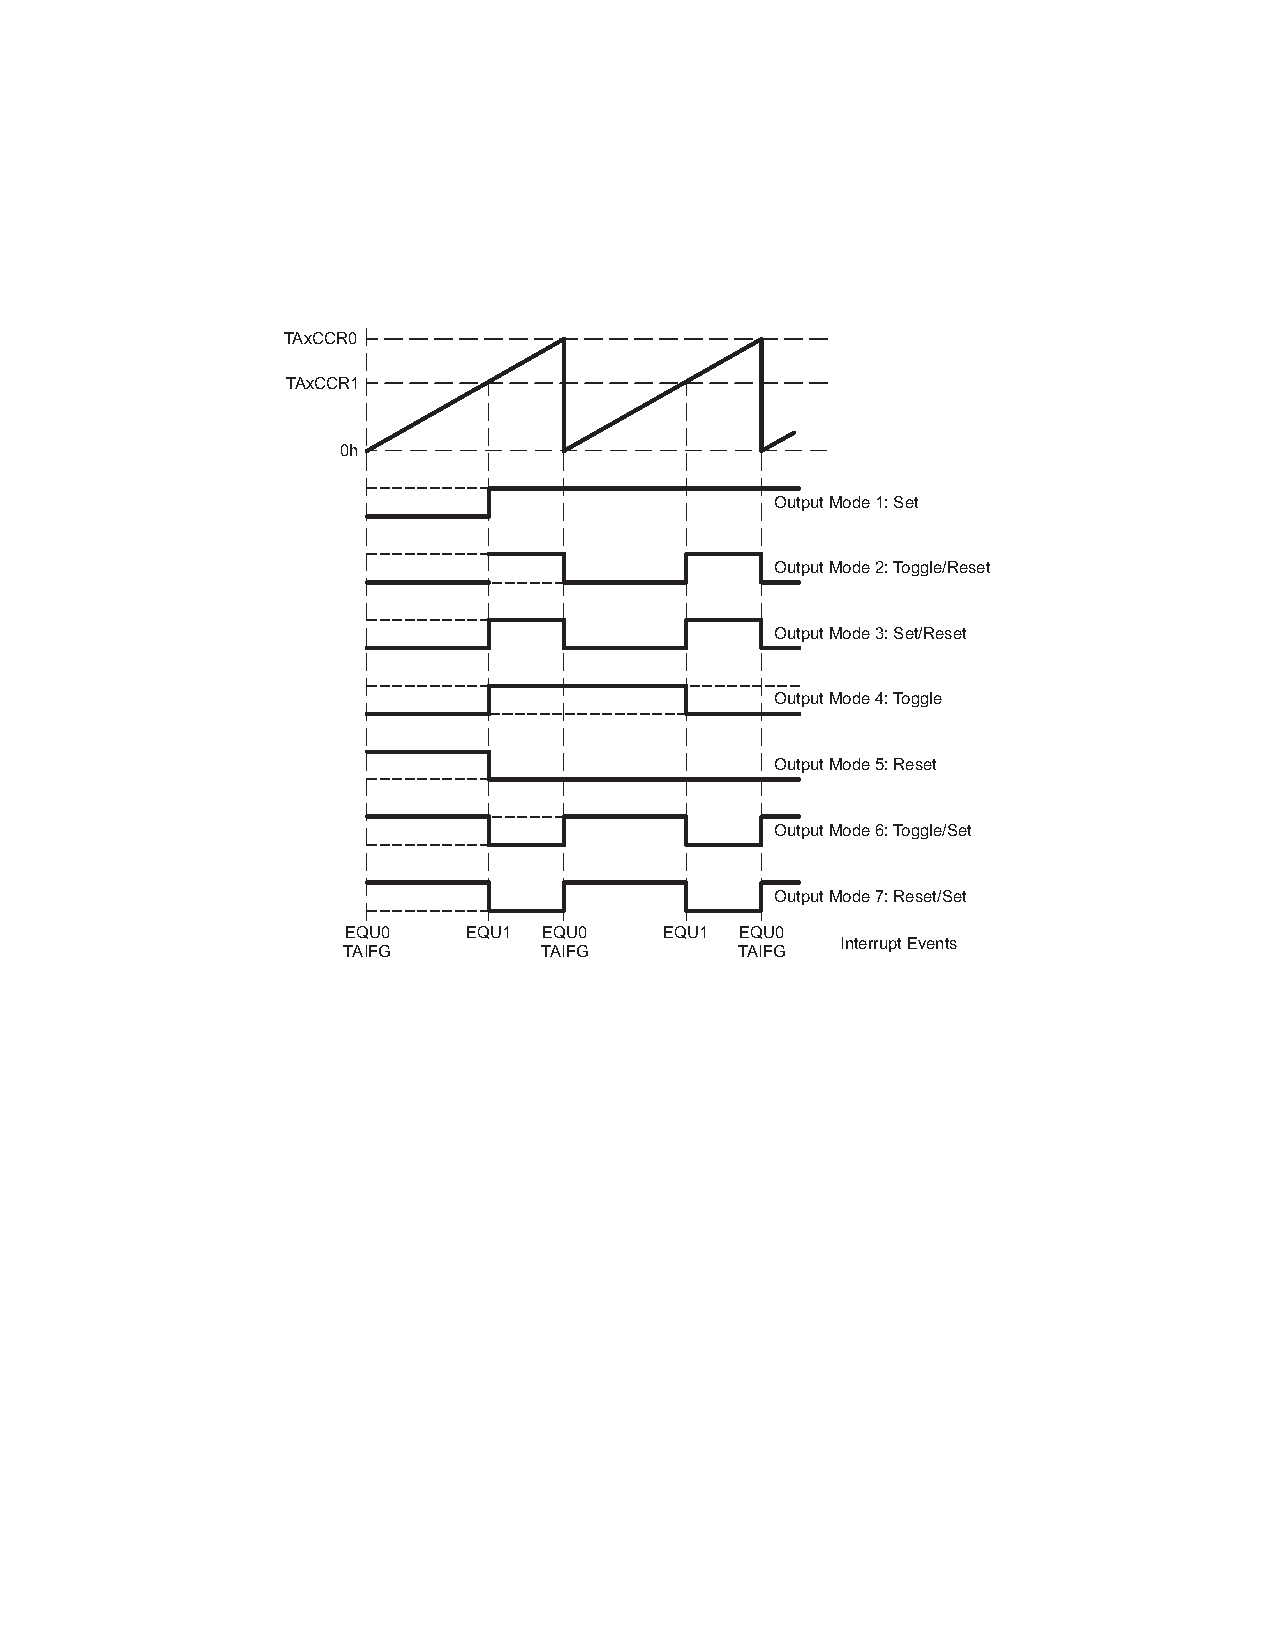
\includegraphics[angle=0, width=14cm]{./Figures/Chap5_Timer/Timer_Out1.pdf}
  \rule{35em}{0.5pt}
  \caption[Outmod_MC1]{Exemple de sortie - TimerA en mode Up (MC = 01)}
  \label{fig:Outmod_MC1}
\end{figure}

\begin{figure}[t]
  \centering
  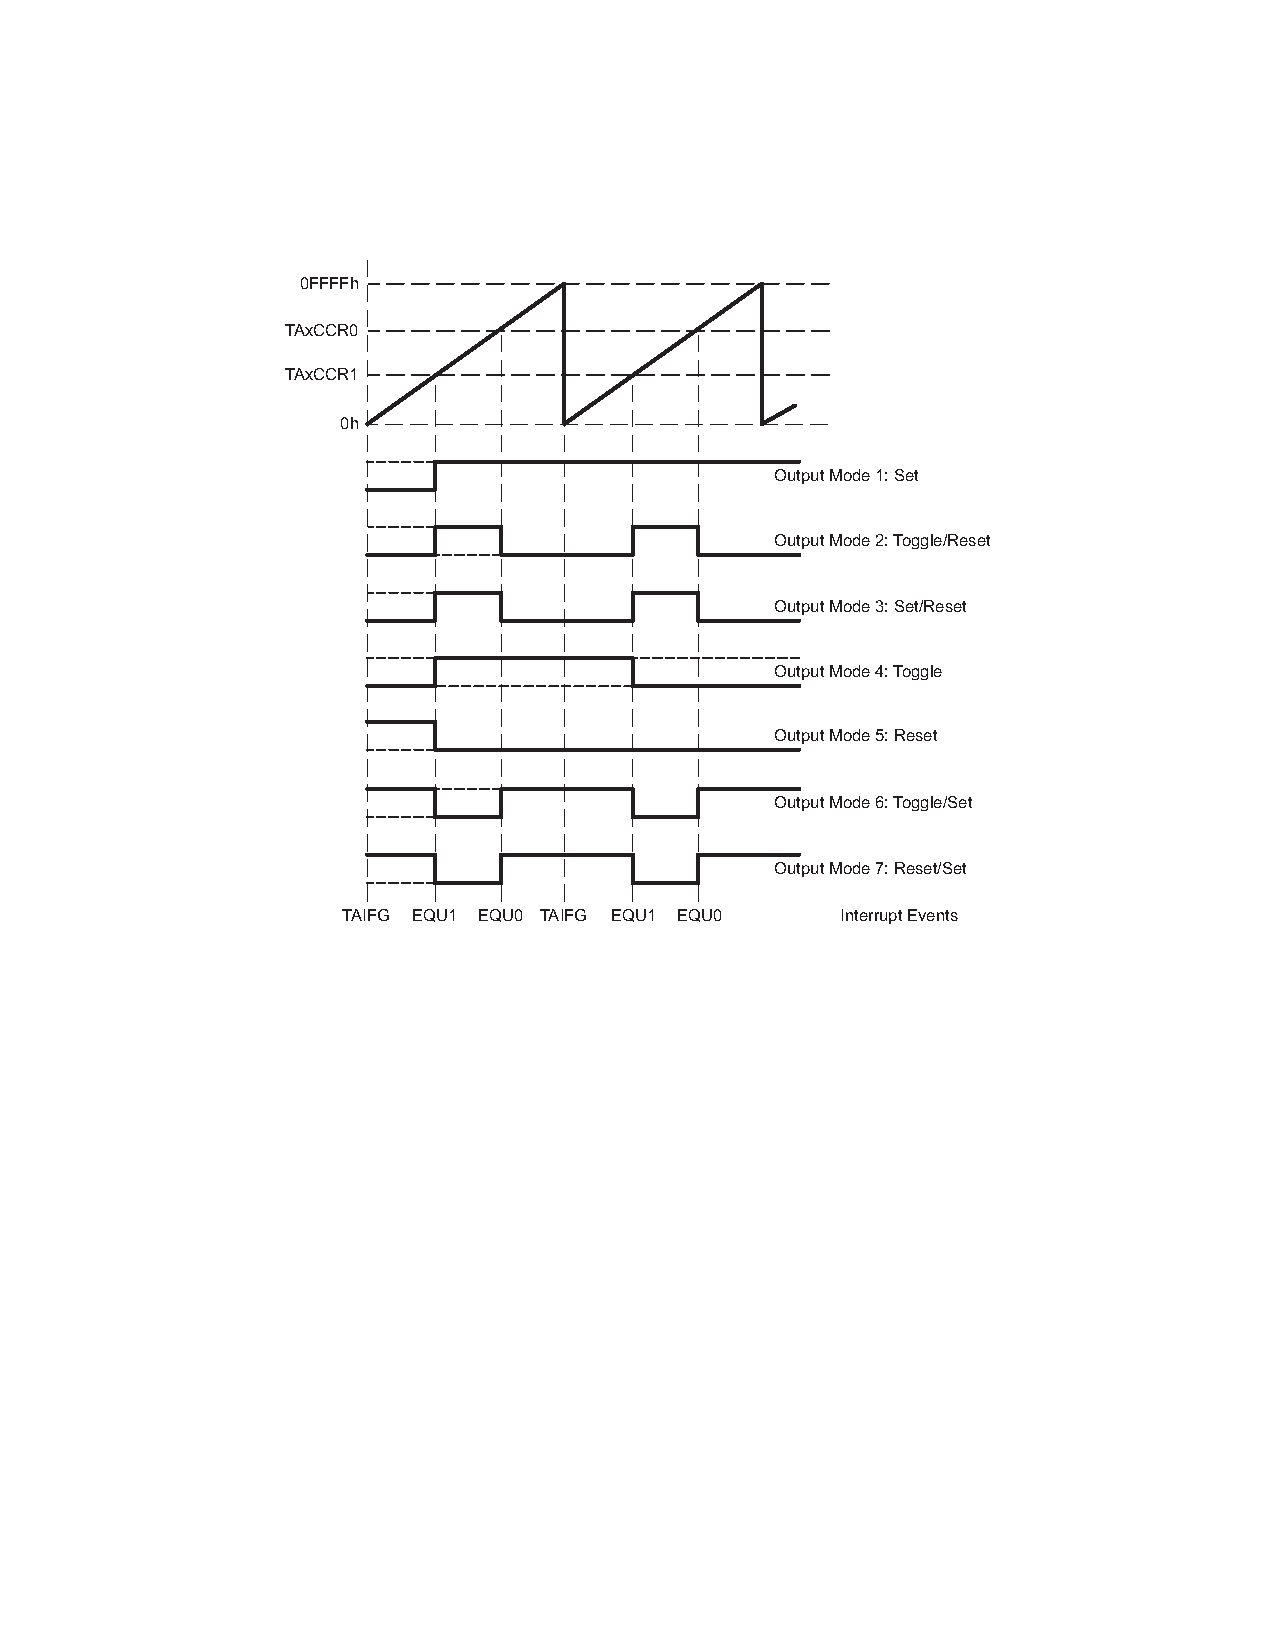
\includegraphics[angle=0, width=14cm]{./Figures/Chap5_Timer/Timer_Out2.pdf}
  \rule{35em}{0.5pt}
  \caption[Outmod_MC2]{Exemple de sortie - TimerA en mode Continu (MC = 10)}
  \label{fig:Outmod_MC2}
\end{figure}

\begin{figure}[t]
  \centering
  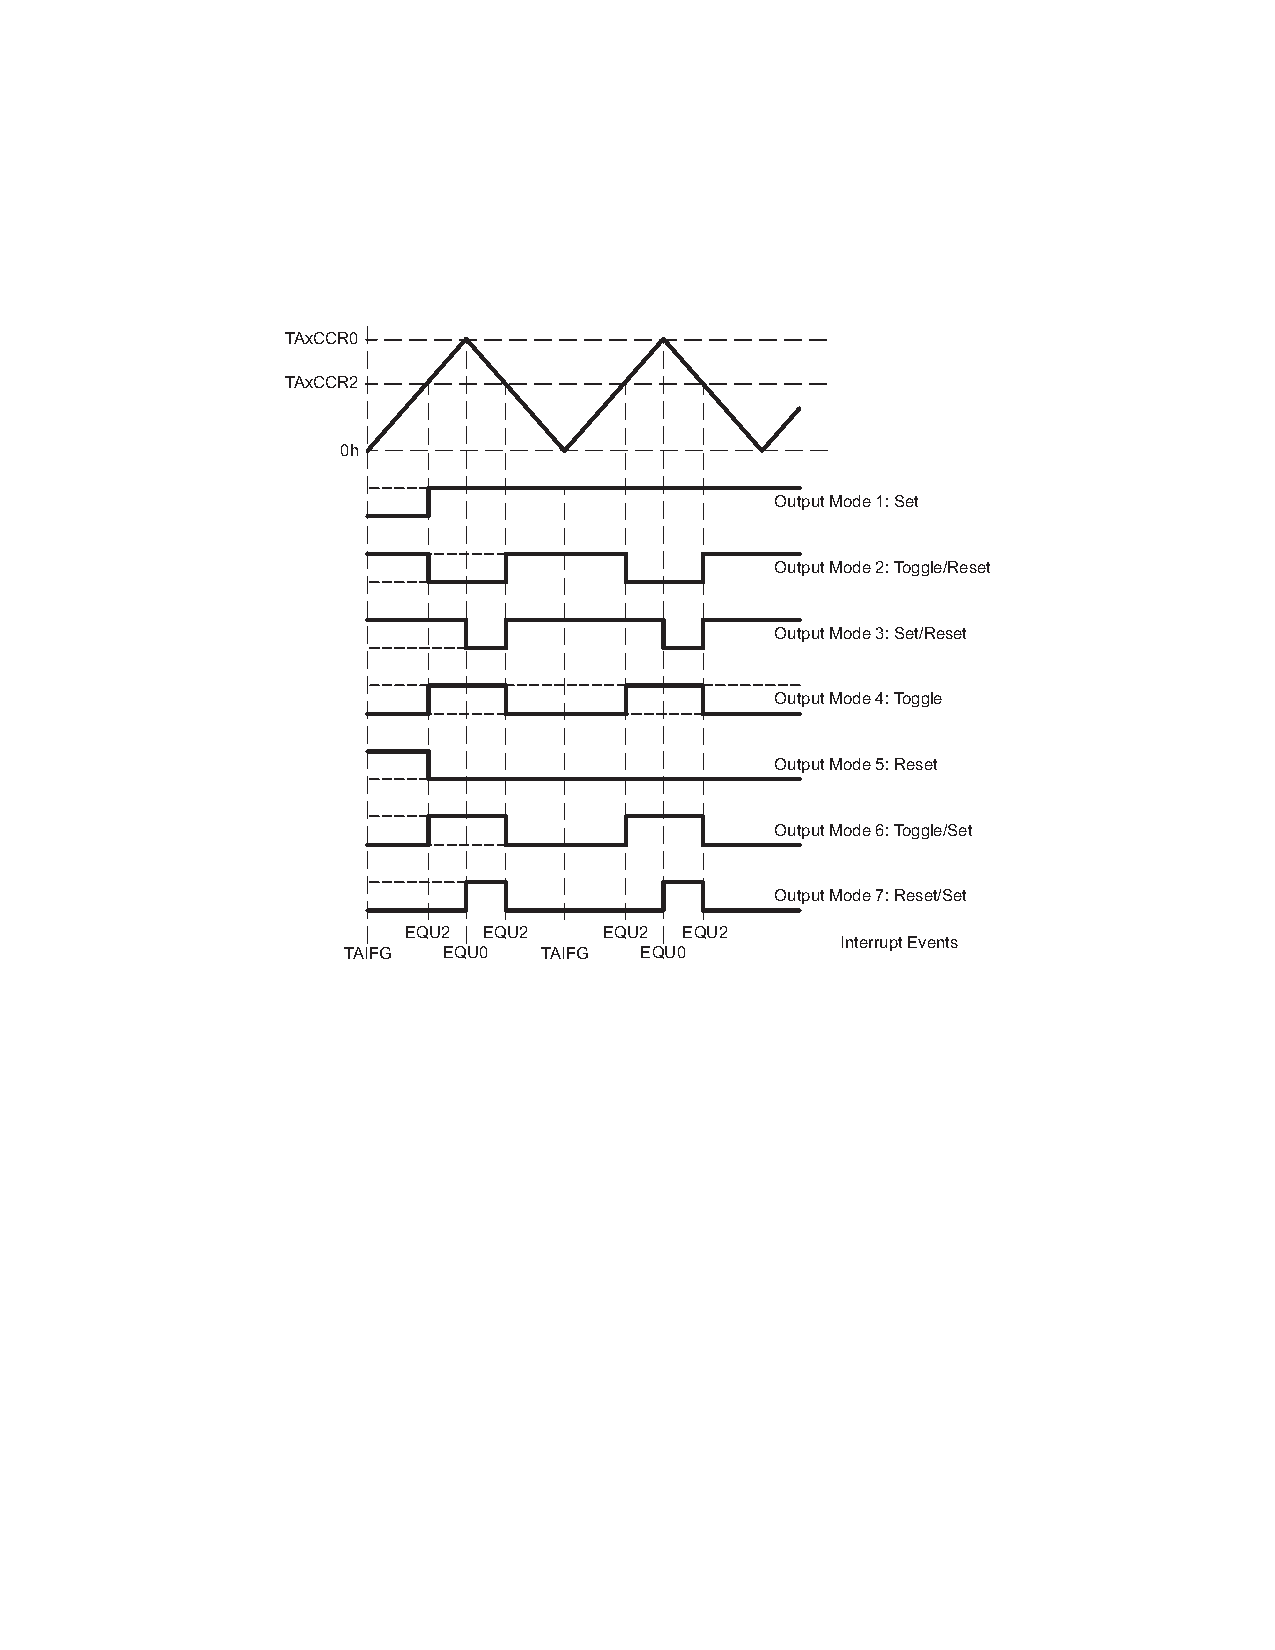
\includegraphics[angle=0, width=14cm]{./Figures/Chap5_Timer/Timer_Out3.pdf}
  \rule{35em}{0.5pt}
  \caption[Outmod_MC3]{Exemple de sortie - TimerA en mode Up/Down (MC = 11)}
  \label{fig:Outmod_MC3}
\end{figure}










\chapter{\textsc{Syst�me d'horloges}}

Comme tout syst�me num�rique, le microcontr�leur et ses p�riph�riques ont besoin d'une horloge. Ce signal contr�le toutes les bascules composant les diff�rentes machines s�quentielles qui composent le syst�me num�rique. La structure d�taill�e de ce type de circuit s�quentiel est �tudi�e au cours "Syst�mes Logiques".

Le signal d'horloge est toujours g�n�r� par un oscillateur, dont les performances d�finissent les qualit�s:
\begin{itemize}[label=\textbullet,font=\small]
\item fr�quence;
\item pr�cision;
\item stabilit�.
\end{itemize}

\section{Oscillateurs}
On distingue 4 types d'oscillateur. Ceux-ci se diff�rencient par le m�canisme donnant naissance � l'oscillation et par les composants externes mis en oeuvre:
\begin{itemize}[label=\textbullet,font=\small]
\item oscillateurs RC (consulter le cours de "Electronique Analogique");
\item oscillateurs � r�sonateur c�ramique ou � quartz;
\item circuits oscillateurs sp�cifiques, �ventuellement calibr�s en usine et � compensation des effets de temp�rature;
\item circuits cal�s sur des signaux externes tels que GPS, dont la pr�cision est obtenue par des horloges atomiques.
\end{itemize}

Dans les microcontr�leurs, on rencontre les deux premiers types.
Tr�s souvent, un multiplicateur de fr�quence permet de g�n�rer une horloge � plus haute fr�quence que ce que les oscillateurs produisent.

\subsection{Oscillateurs RC}
L'oscillateur RC le plus simple est probablement celui illustr� � la figure \ref{fig:Osc_RC_1}. Il est bas� sur un inverseur logique � hyst�r�se ou \textit{Trigger de Schmitt}, une r�sistance et une capacit�.

\begin{figure}[htb]
  \centering
  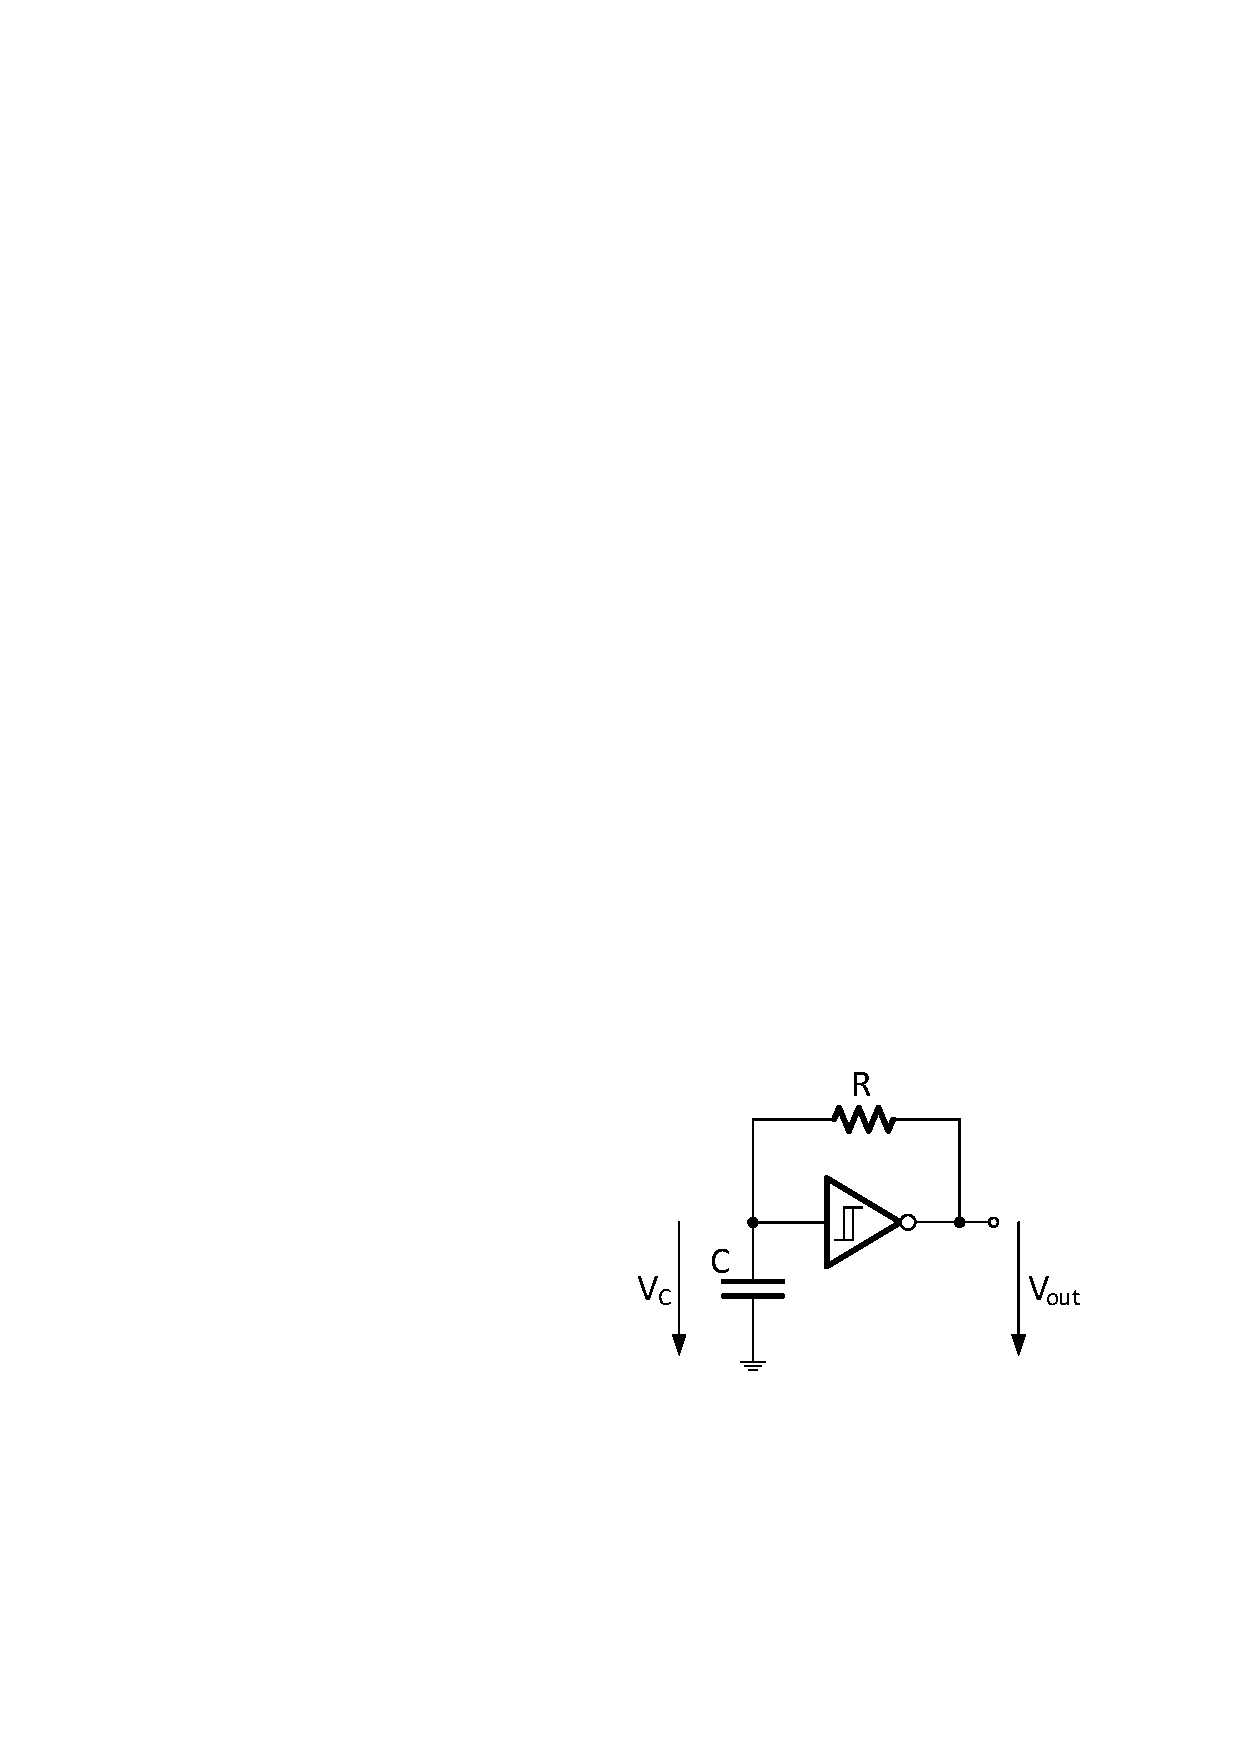
\includegraphics [angle=0, width=8cm]{./Figures/Chap6_Horloges/Osc_RC_1.pdf}
  \rule{35em}{0.5pt}
  \caption[Sch�ma Timer]{Oscillateur RC � Trigger de Schmitt}
  \label{fig:Osc_RC_1}
\end{figure}

La figure \ref{fig:Osc_RC_2} illustre les signaux � l'entr�e et � la sortie de l'inverseur � hyst�r�se.

\begin{figure}[htb]
  \centering
  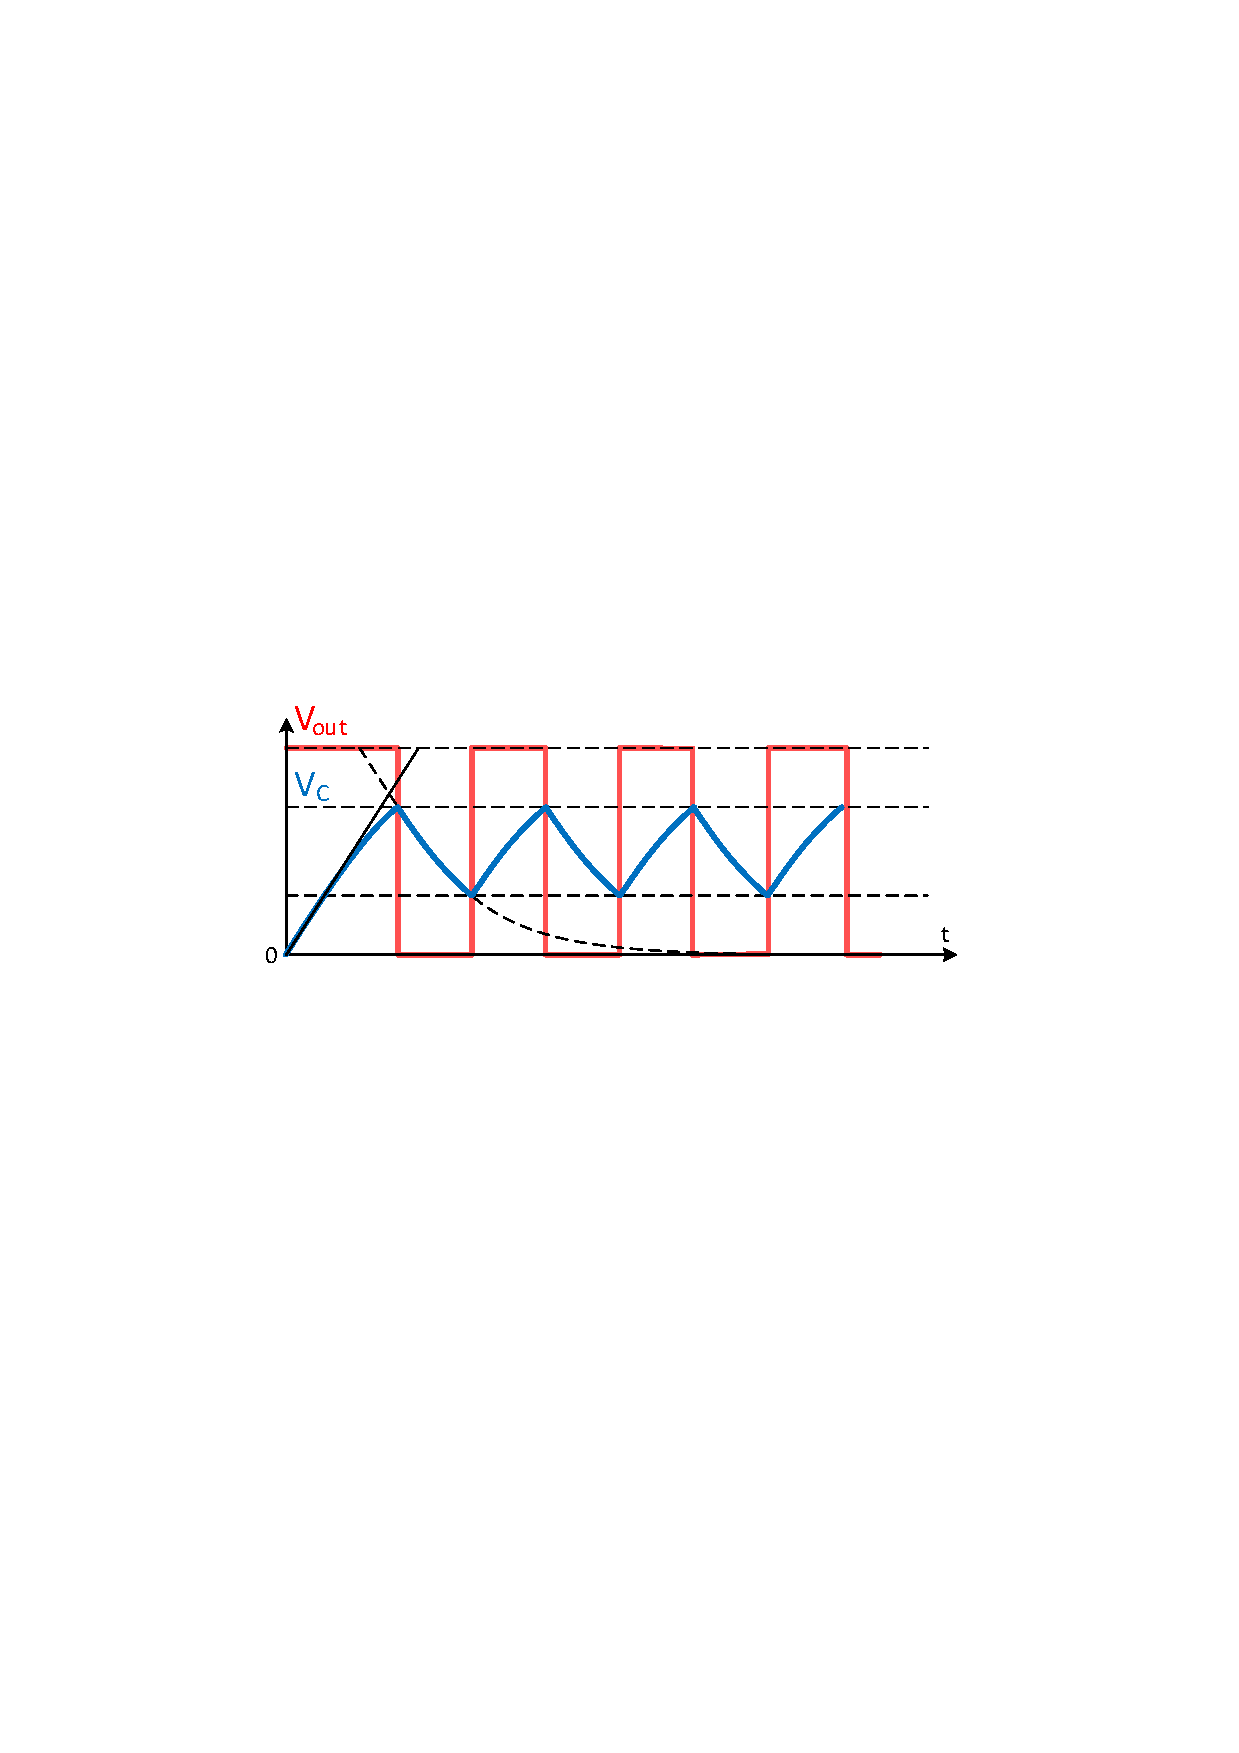
\includegraphics [angle=0, width=14cm]{./Figures/Chap6_Horloges/Osc_RC_2.pdf}
  \rule{35em}{0.5pt}
  \caption[Sch�ma Timer]{Signal de l'oscillateur RC}
  \label{fig:Osc_RC_2}
\end{figure}

Du fait de la faible pr�cision de la valeur des composants, tant la r�sistance, la capacit� que les seuils d'hyst�r�se, la fr�quence de l'oscillation est peu pr�cise et peu stable en temp�rature. Par contre, tous les composants peuvent �tre int�gr�s. C'est pourquoi on rencontre ce type d'oscillateur dans la plupart des microcontr�leurs modernes, pour toutes les applications qui ne n�cessitent pas une fr�quence pr�cise.

\subsection{Oscillateurs � quartz}
Si la fr�quence doit �tre pr�cise, l'oscillateur � quartz est le circuit le plus couramment utilis�. Son fonctionnement est bas� sur l'utilisation d'un cristal pi�zo�lectrique, dans lequel l'�nergie est stock�e soit sous forme m�canique soit sous forme �lectrique. L'oscillation consiste en un �change alternatif entre l'�nergie m�canique et l'�nergie �lectrique. Le circuit oscillateur entretient l'oscillation, en compensant les pertes d'�nergie qui sont tr�s faibles. Le sch�ma typique d'un oscillateur � quartz est donn� � la figure \ref{fig:Osc_XTAL_1}.

\begin{figure}[htb]
  \centering
  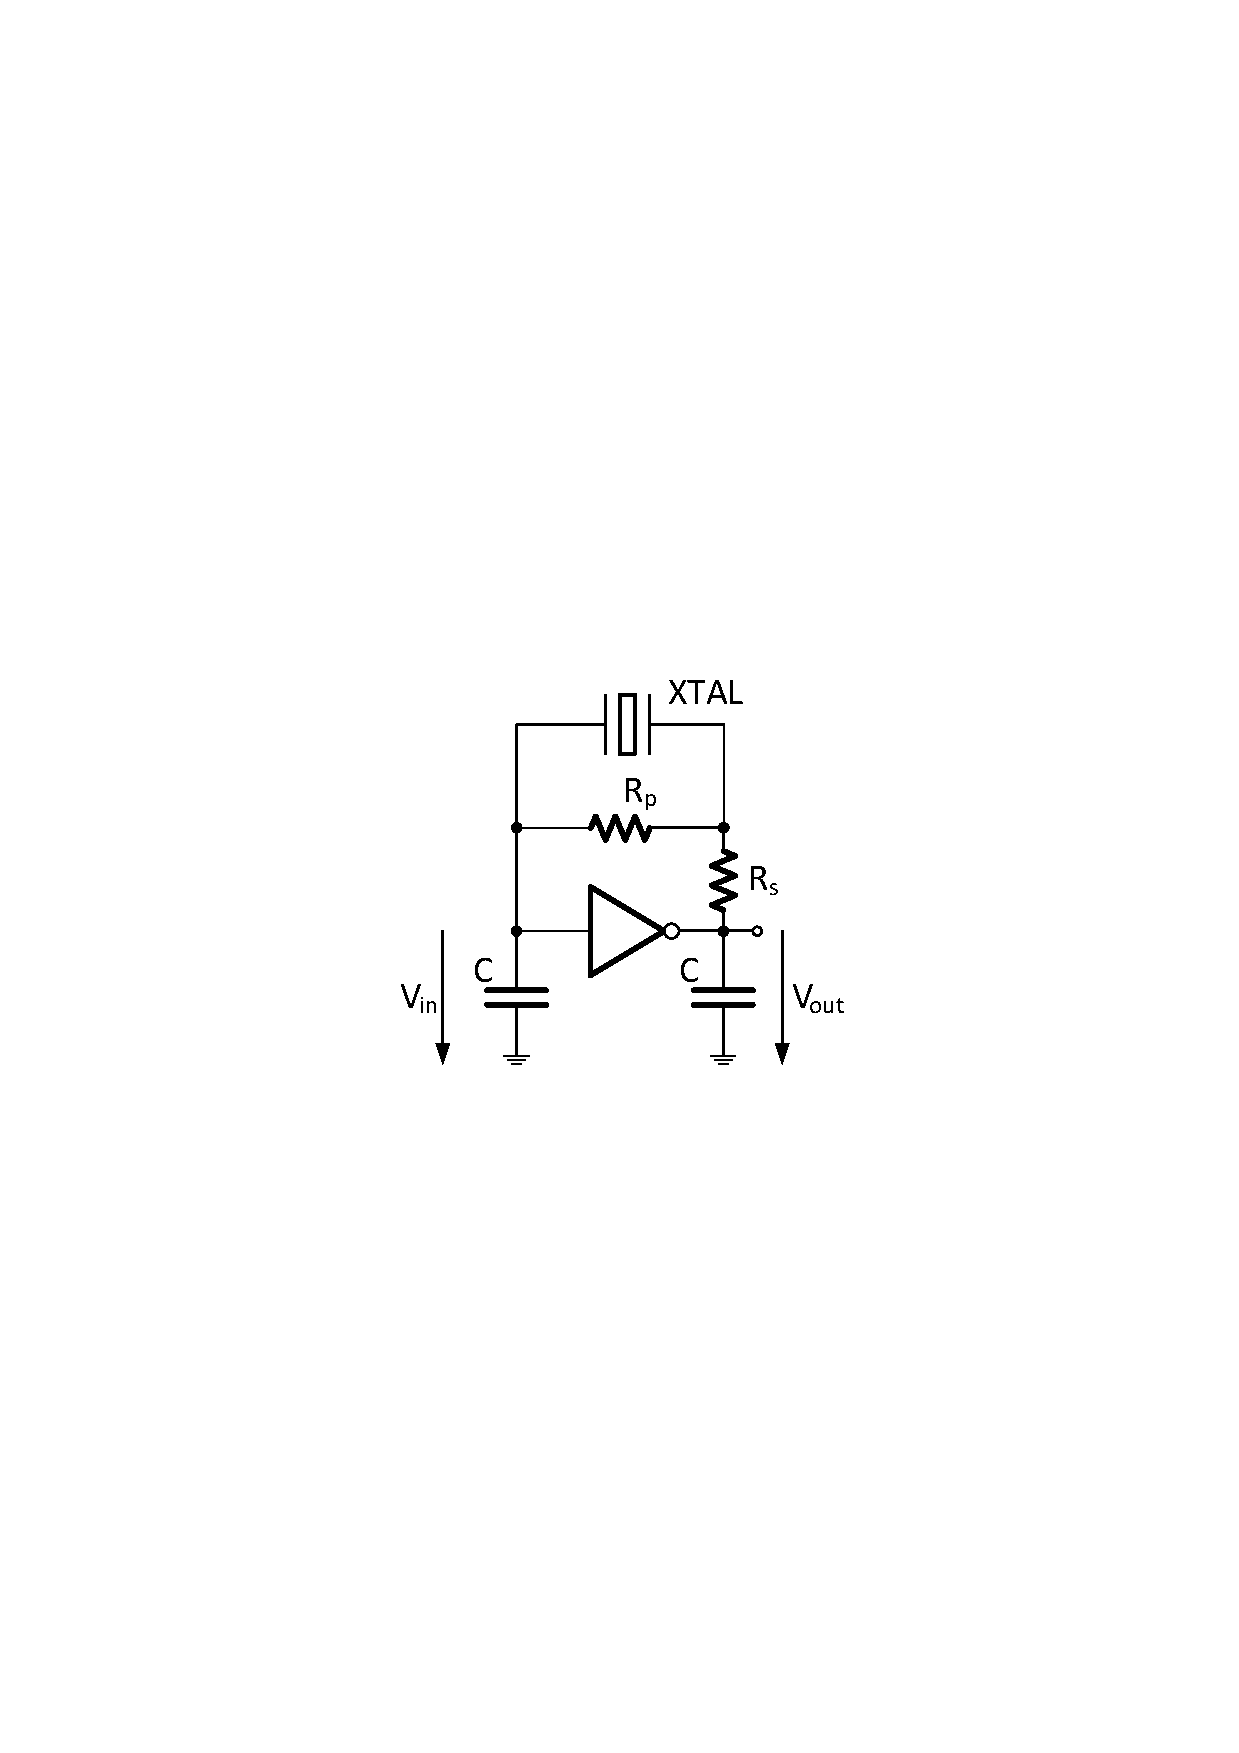
\includegraphics [angle=0, width=8cm]{./Figures/Chap6_Horloges/Osc_XTAL_1.pdf}
  \rule{35em}{0.5pt}
  \caption[Sch�ma Timer]{Sch�ma de l'oscillateur � quartz}
  \label{fig:Osc_XTAL_1}
\end{figure}

Dans ce circuit, la r�sistance a une grande valeur et ne sert qu'� polariser l'inverseur logique � son point de repos donnant le gain maximal. Ainsi connect�, l'inverseur maintien le r�sonateur en oscillation (figure \ref{fig:Osc_RC_1}). Le signal de sortie de l'inverseur est ensuite transform� en un signal carr� qui constitue l'horloge de base pour le reste du circuit.

Une variante du r�sonateur � quartz est le r�sonateur c�ramique. Son fonctionnement est similaire � celui du quartz. Il se justifie pour son co�t moindre, au prix de performances moindres.

\subsection{Crit�res de performance des oscillateurs}
Un oscillateur est caract�ris� par:
\begin{itemize}[label=\textbullet,font=\small]
\item sa fr�quence;
\item la pr�cision de la fr�quence;
\item la stabilit� instantan�e de la fr�quence, qui est li�e au facteur de qualit�;
\item la stabilit� de la fr�quence dans le temps.
\end{itemize}

\subsubsection*{Fr�quence}
Dans un oscillateur RC, la fr�quence est peu pr�cise car elle d�pend de composants dont les valeurs sont peu pr�cises. Dans un oscillateur � r�sonateur, la fr�quence est essentiellement d�termin�e par le r�sonateur. Sa fr�quence de r�sonance a une erreur relative, sp�cifi�e en \textit{ppm}, ou \it part par million \rm. Un cristal de qualit� moyenne a une erreur de fr�quence de 100 ppm, soit 0,001%.

\subsubsection*{Facteur de qualit�}
Le facteur de qualit� du signal est d�fini par $Q=\frac{f_{c}}{BW}$.
Si Q est grand, la bande passante est petite par rapport � la fr�quence centrale de l'oscillation et donc la stabilit� en fr�quence est grande.

\subsubsection*{Stabilit�}
La stabilit� en fr�quence d'un r�sonateur est aussi donn�e en ppm.
La fr�quence suit les d�rives des composants. On distingue trois types de d�rives :
\begin{itemize}[label=\textbullet,font=\small]
\item le vieillissement des composants, de l'ordre de 5 � 50 ppm;
\item l'effet des variations de temp�rature, de l'ordre de 20 � 200 ppm;
\item l'effet des variations d'humidit�, en g�n�ral inf�rieure � 10 ppm.
\end{itemize}

Ces trois effets sont li�s � la nature m�canique du r�sonateur. Le vieillissement peut �tre associ� au rel�chement de tensions m�caniques internes au cours du temps. La temp�rature modifie les dimensions physiques du r�sonateur � cause de la dilatation. L'humidit� diffuse dans le mat�riau lui-m�me.

\section{Multiplicateur de fr�quence}
Un multiplicateur de fr�quence contient deux fonctions de base :
\begin{itemize}[label=\textbullet,font=\small]
\item g�n�ration "libre" d'un signal � une fr�quence proche de la fr�quence vis�e;
\item asservissement de la fr�quence obtenue � une fr�quence de r�f�rence
\end{itemize}



\subsection{Zip} 

\begin{figure}[htb]
  \centering
  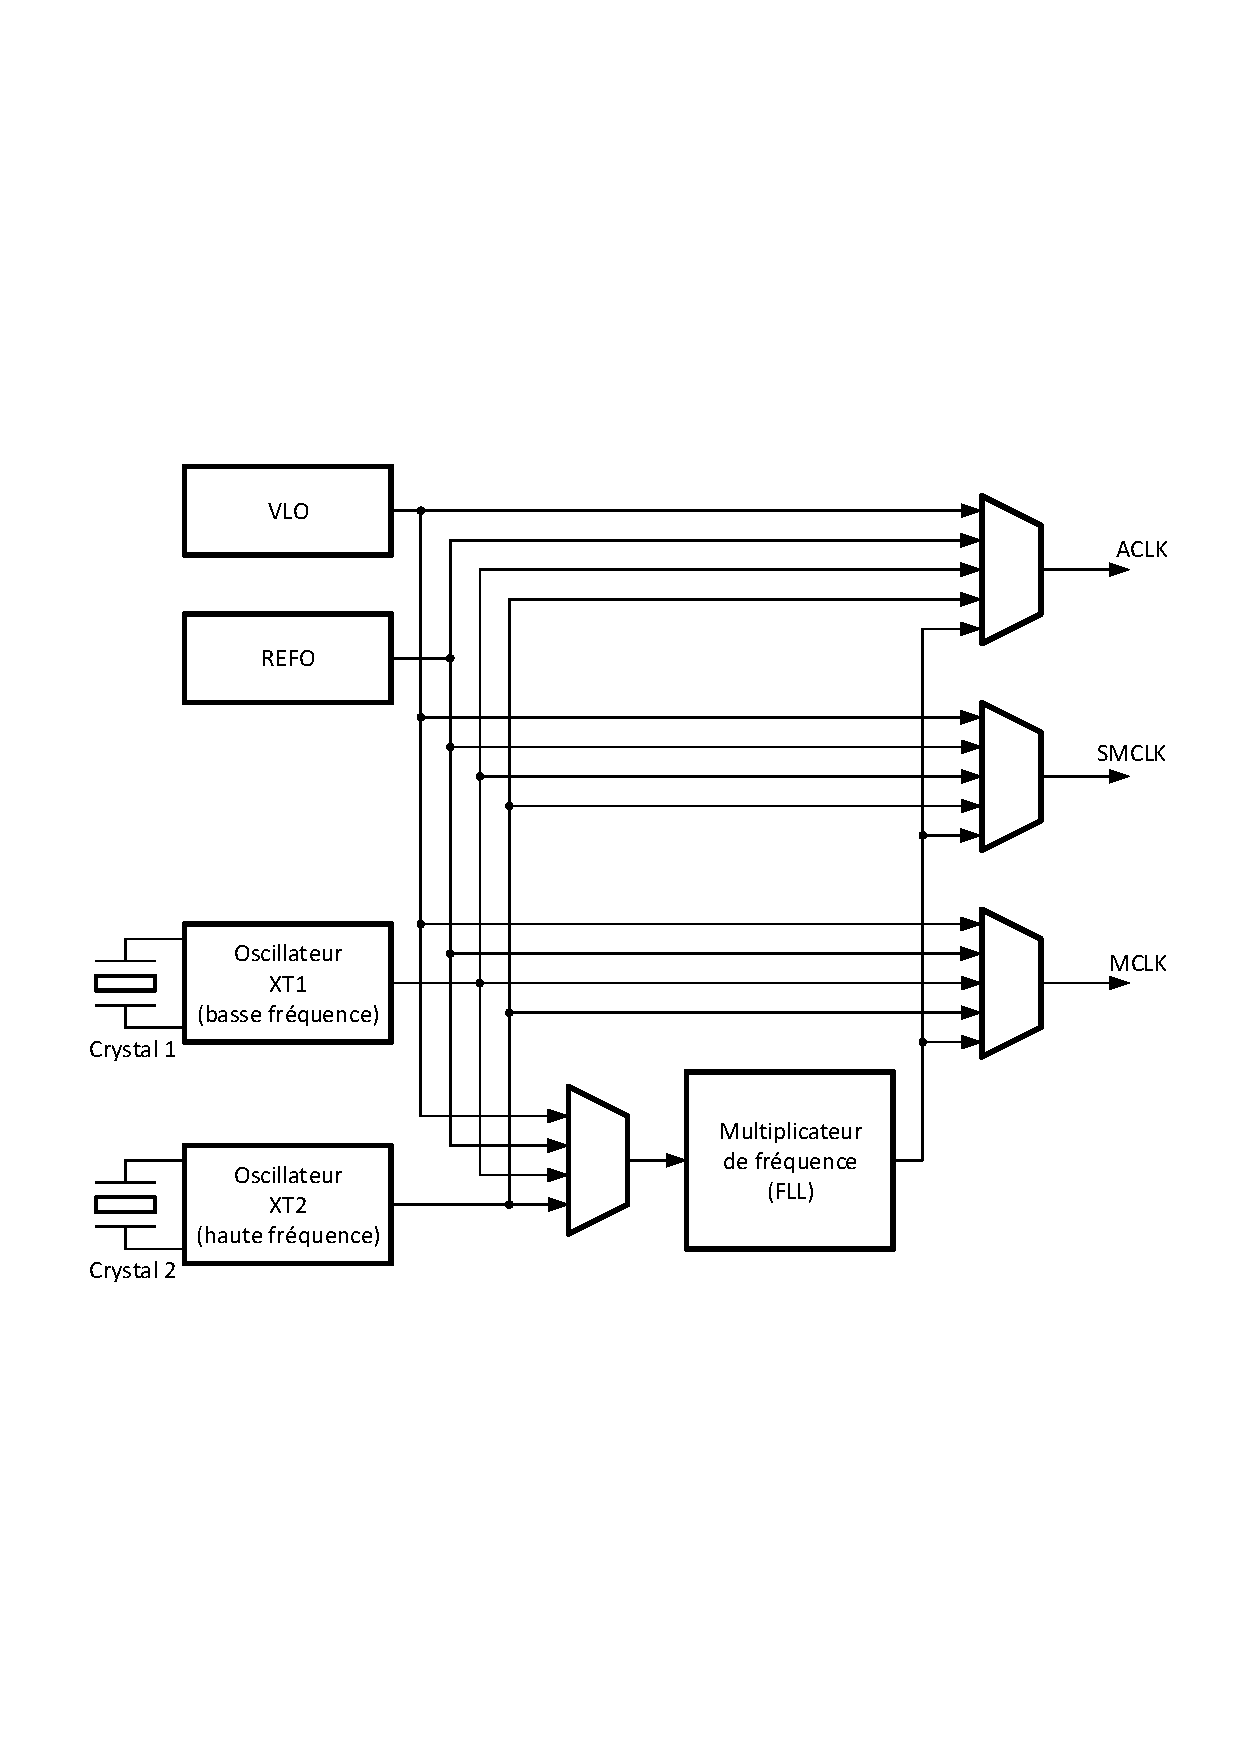
\includegraphics [angle=0, width=14cm]{./Figures/Chap6_Horloges/UCS_Blocs.pdf}
  \rule{35em}{0.5pt}
  \caption[Sch�ma Timer]{Sch�ma synoptique du circuit d'horloge du MSP430}
  \label{fig:UCS_Blocs}
\end{figure}







\chapter{\textsc{Assembleur}}

On appelle \textit{langage machine} le langage natif du CPU, c'est � dire le langage qui peut �tre directement \textit{interpr�t�} par le processeur. Les instructions sont des mots binaires organis�s en champs, qui commandent chacun des actions sp�cifiques telles que :
\begin{itemize}[label=\textbullet,font=\small]
\item le type d'op�ration � effectuer
\item les op�randes
\item le mode d'adressage
\end{itemize}
Le langage machine est donc intrins�quement li� au CPU auquel il s'applique,

Le langage d'assemblage (ou langage assembleur ou simplement assembleur par abus de
langage, abr�g� ASM) est une version lisible du langage machine. Il consiste � repr�senter les codes binaires des instructions par des symboles appel�s mn�moniques (du grec mn�monikos, relatif � la m�moire), c'est-�-dire faciles � retenir.

Par exemple, l'unit� de contr�le d'un processeur particulier reconna�t l'instruction en langage
machine suivante :

%MOV R0,#data	0x78
%\begin{tabbing}
%\qquad 01111000 01010101 b en binaire\\
%\qquad 0x78 0x55 en hexad�cimal
%\end{tabbing}

\begin{tabbing}
\qquad 01000000 00110101 00000000 01010101 b en binaire\\
\qquad 4035 0055h en hexad�cimal
\end{tabbing}

On voit bien qu'il est impossible de comprendre directement ce que peut faire cette instruction.
En langage assembleur, cette instruction est traduite par un �quivalent plus facile � comprendre
pour le programmeur :
\begin{tabbing}
\qquad MOV.W   \#85,R5
\end{tabbing}

qui signifie "mettre la valeur d�cimale 85" (0x55 en hexad�cimal) dans le registre R5.

\section{Jeu d'instructions}
Le jeu d'instructions est l'ensemble de toutes les instructions que le CPU est capable d'ex�cuter. On peut en g�n�ral les regrouper en plusieurs cat�gories:
\begin{itemize}[label=\textbullet,font=\small]
\item instructions de transfert de donn�es; elles consistent � copier le contenu d'un registre ou d'une case m�moire vers un autre registre ou une autre cas m�moire.
\item op�rations arithm�tiques;
\item op�rations logiques;
\item sauts et rupture de s�quence contr�l�s ou non par un test, qui permettent (par exemple) de faire des appels de sous-programme.
\end{itemize}

Le jeu d'instruction d'un CPU peut �tre plus ou moins complet selon la complexit� du CPU. Par exemple, celui de la famille MCS-51 (famille de microcontr�leurs Intel 8051 et 8052) comprend environ 110 instructions, alors que le MSP430 a "seulement" 27 instructions, tout en offrant des performances comparables.
La raison est li�e au\it mode d'adressage\rm, qui d�finit la fa�on dont le CPU acc�de aux donn�es qu'il s'appr�te � traiter, que ce soit pour un simple transfert de donn�es ou une op�ration arithm�tique sophistiqu�e.

\section{Mode d'adressage}
Selon que l'op�rande d'une instruction est une constante, une variable, un pointeur ou autre, il est �vident que cet op�rande n'est pas identifi� de la m�me mani�re.
Reprenant l'instruction prise comme exemple dans l'introduction:
\begin{tabbing}
\qquad MOV.W   \#85,R5
\end{tabbing}
la valeur "85", qui �tait cod�e par "0055" pourrait repr�senter:
\begin{itemize}[label=\textbullet,font=\small]
\item le nombre (la constante) 85;
\item la case m�moire num�ro 85;
\item si c'est la case m�moire num�ro 85, est-ce son contenu qui est l'op�rande ou autre chose ?
\item etc...
\end{itemize}

M�me si les modes d'adressage varient grandement d'un CPU � un autre, on peut en identifier quelques uns qui leurs sont communs.

\subsection{Adressage imm�diat}
En adressage \textit{imm�diat}, la donn�e est identifi�e explicitement. Dans l'exemple d�j� vu 
\begin{tabbing}
\qquad MOV.W   \#85,R5
\end{tabbing}
le symbole \# sp�cifie que la valeur est � prendre telle quelle.
L'adressage imm�diat est donc associ� � une constante.

\subsection{Adressage direct}
En adressage \textit{direct}, l'identifiant est l'adresse de la case contenant la donn�e. L'exemple devient
\begin{tabbing}
\qquad MOV.W   85,R5
\end{tabbing}
C'est l'adressage "par d�faut", le plus courant, sp�cifi� par le symbole \& ou par l'absence de symbole. L'adressage direct est donc associ� � une variable. La case m�moire ou le registre identifi� est une variable.

\subsection{Adressage indirect}
En adressage \textit{indirect}, l'identifiant est l'adresse d'une case m�moire, qui contient l'adresse de la donn�e vis�e . L'exemple devient
\begin{tabbing}
\qquad MOV.W   @85,R5
\end{tabbing}
Cet adressage est sp�cifi� par le symbole @. L'adressage indirect permet donc d'impl�menter un pointeur.

\subsection{Adressage index�}
L'adressage \textit{index�} permet de g�rer des tableaux de fa�on efficace. 

\subsection{Orthogonalit� du jeu d'instruction}



\section{Chaine de compilation}


\section{Debug}

\chapter{\textsc{CPU}}

Bla bla bla


\section{Principe}


\subsection{Tada}








\chapter{\textsc{Programmation en C}}
Pour atteindre le matériel depuis un langage de plus haut niveau, il faut un certain nombre d'instructions et de règles pour pouvoir rester dans un ensemble cohérent.


\section{Programmation système et programmation applicative}
Les règles de programmation sont différentes si on écrit du code relatif à du matériel par rapport à des applications purement logiciel. Le premier exemple, déjà traité au chapitre 4, est les interruptions. Ce sont des fonctions système que l'on trouve seulement lorsqu'on programme à bas niveau. 

\begin{table}[!htbp]
\begin{center}
{\fontfamily{phv}\selectfont
\begin{tabular}{|c|c|}
\hline 
Programmation Système & Programmation Applicative \\
\hline  
\hline 
Interruptions & Pas d'interruptions \\
\hline 
Variables globales & Éviter les variables globales\\
\hline
Langages de bas niveau & Langages de haut niveau\\
\hline
Structuration faible & Structuration forte\\
\hline
\end{tabular}
}
\end{center}
\caption{Comparaison des styles de programmation \label{prog}}
\end{table}

\section{Directives et variables spécifiques à la programmation système}

\subsection{Variables volatiles}
Dans le cas ou une zone de stockage, tel qu'un registre, peut être modifié par autre chose que le programme principal on doit lui attribuer le modificateur volatile. Cela permet au compilateur de savoir que cette variable peut changer même si le code n'affecte jamais cette variable. Le compilateur ne va donc pas essayer d'optimiser une variable volatile (Exemple ci-dessous). 

\subsection{Directive pragma}
La directive \#pragma est une commande de précompilation définie par le standard ISO/ANSI C. Elle permet de garder une certaine portabilité du logiciel en contrôlant de manière particulière les extensions spécifiques à un fabricant. Cette directive permet, par exemple, de spécifier une adresse absolue qui désigne la position mémoire pour la déclaration suivante. La variable doit être déclarée soit \_\_no\_init ou const. 

\lstset{style=customc}
\begin{lstlisting}
#pragma location=0x22E
__no_init volatile char PORT1;	//PORT1 est un registre du périphérique
                                //du même nom placé à l'adresse 0x22E
\end{lstlisting}
La directive \#pragma peut prendre d'autres fonctions selon le compilateur utilisé.

\subsection{Fonctions intrinsèques}
Les fonctions intrinsèques se reconnaissent par un double souligné devant (\_\_). Les fonctions intrinsèques permettent un accès direct aux instructions de bas niveau sans programmer en assembleur. Si le compilateur ne trouve pas les fonctions intrinsèques par défaut alors il faut inclure: intrinsics.h. Ces fonctions ne sont pas standard, elle dépendent du compilateur utilisé.

Exemple de fonctions intrinsèques:
\lstset{style=customc}
\begin{lstlisting}
__no_init					//indique de ne pas initialiser une variable
__disable_interrupt			//désactive toutes les interruptions
__enable_interrupt			//active toutes les interruptions
__low_power_mode_n			//enclenche le mode low power n
__low_power_mode_off_on_exit //désactive le mode low power en sortie d'interruption
__asm()						//permet l'insertion de code assembleur
\end{lstlisting}


\section{Librairies d'abstraction du matériel: HAL}
Pour rendre l'écriture de programmes plus propre on peut ajouter de la hiérarchie. Une façon de faire est de placer toutes les fonctions relatives aux périphériques dans des librairies d'abstraction de matériel ou HAL (Hardware Abstraction Library).

Une librairie HAL doit permettre de masquer tout ce qui est relatif à un périphérique donné. La structure typique d'un HAL est la suivante:
\begin{itemize}
\item Constantes spécifiques
\item Variables spécifiques
\item Une fonction d'initialisation du périphérique
\item Une fonction de mise en veille ou désactivation
\item Des fonctions spécifiques comme lecture ou écriture
\end{itemize}

Exemples de structure HAL pour un accéléromètre (CMA3000):
\lstset{style=customc}
\begin{lstlisting}
#define CTRL                    0x02
#define MODE_400                0x04        // Measurement mode 400 Hz ODR

int8_t Cma3000_xAccel;
int8_t Cma3000_yAccel;
int8_t Cma3000_zAccel;

void Cma3000_init(void)
{
	...
}

void Cma3000_disable(void)
{
	...
}

void Cma3000_readAccel(void)
{
	...
} 

...
\end{lstlisting}

Les interruptions relatives à un périphérique doivent être aussi traitées dans le HAL.

\section{Pilotes}
Un pilote ou driver permet la gestion d'un périphérique dans le cadre d'un système d'exploitation. C'est un HAL avec en plus les interfaces standards propre à un système d'exploitation. Il existe donc des standards pour écrire des pilotes. 

\section{Contrôle de l'exécution}

Dans le cadre d'une programmation simple (mono-tâche), le processeur effectue les instructions linéairement à sa vitesse maximale. On a donc des instants actifs, avec des instructions à exécuter, et des instants inactifs où il n'y a rien à faire. Dans le cas le plus simple, la partie inactive est une attente active ou le processeur exécute une boucle infinie genre: while(1). Ceci revient à faire le même test qui est toujours vrai et donc à gaspiller de l'énergie. Il est de ce fait plus intéressant de mettre le processeur en pause. Ceci implique qu'il faut gérer le réveil au moment requis par le système.

Le cycle actif/pause peut être géré de deux manières:
\begin{enumerate}
\item Par interruption, une requête externe par exemple
\item Par un timer, réveil à intervalle régulier.
\end{enumerate}

Exemple de code pour MSP430 dans le cas (1):
\lstset{style=customc}
\begin{lstlisting}
void main(void) {
	while(1) {
		__bis_SR_register(LPM3_bits + GIE);	//Mode basse consommation LPM3 
											//avec interruptions activées
		...									//Code de l'application, 
											//mode low power!
	}
}

#pragma vector=PORT2_VECTOR
__interrupt void Port2_ISR(void) {

	...										//Code de l'interruption, 
											//mode actif par défaut
	__low_power_mode_off_on_exit	
}
\end{lstlisting}

Pour bien comprendre le code ci-dessus, il faut savoir qu'une interruption est toujours exécutée en mode actif (pas low power) et que dès la sortie, le processeur retourne dans le mode d'avant l'interruption. Il faut donc utiliser la fonction intrinsèque \_\_low\_power\_mode\_off\_on\_exit pour retourner dans le programme principal en mode actif et exécuter le code de l'application. Le mécanisme qui régit cette opération est la sauvegarde du contexte qui sauve sur la pile le registre de statut SR lors de l'interruption puis le dépile lors de la sortie. Rappel: les modes basse consommation sont désignés dans le SR.

Exemple de code pour MSP430 dans le cas (2):
\lstset{style=customc}
\begin{lstlisting}
void main(void) {
	while(1) {		
		__bis_SR_register(LPM3_bits + GIE);	//Mode basse consommation LPM3 
											//avec interruptions activées
		...									//Code de l'application, 
											//mode low power!
	}
}

#pragma vector=TIMER_A0_VECTOR
__interrupt void Timer_ISR(void) {

	...										//Code de l'interruption, 
											//mode actif par défaut
	__low_power_mode_off_on_exit	
}
\end{lstlisting}
 

\chapter{\textsc{Interfaces s�ries}}

Les interfaces parall�les ne sont quasiment plus utilis�es aujourd'hui � cause du nombre de broches n�cessaires et des performances �lectriques demand�es. L'interface s�rie n'utilise que 2 ou 3 broches et b�n�ficie de meilleur performances. Elles demandent, par contre, plus de mat�riel et de logiciel pour effectuer la s�rialisation et d�-s�rialisation.


\section{Notion de pile protocolaire}
Il est utile d'inscrire les interfaces s�ries au sein des notions de la t�l�informatique comme celle de la pile protocolaire. Cette pile permet de d�couper toutes les op�rations n�cessaires en couches. Chaque couche � une fonction bien pr�cise et est d�velopp�e ind�pendamment des autres. 

\subsection{Mod�le OSI (Open Systems Interconnection)}
Le mod�le OSI est un mod�le th�orique d'une pile de communication avec sept couches (fig. \ref{fig:osi}). 

\begin{figure}[htb]
  \centering
  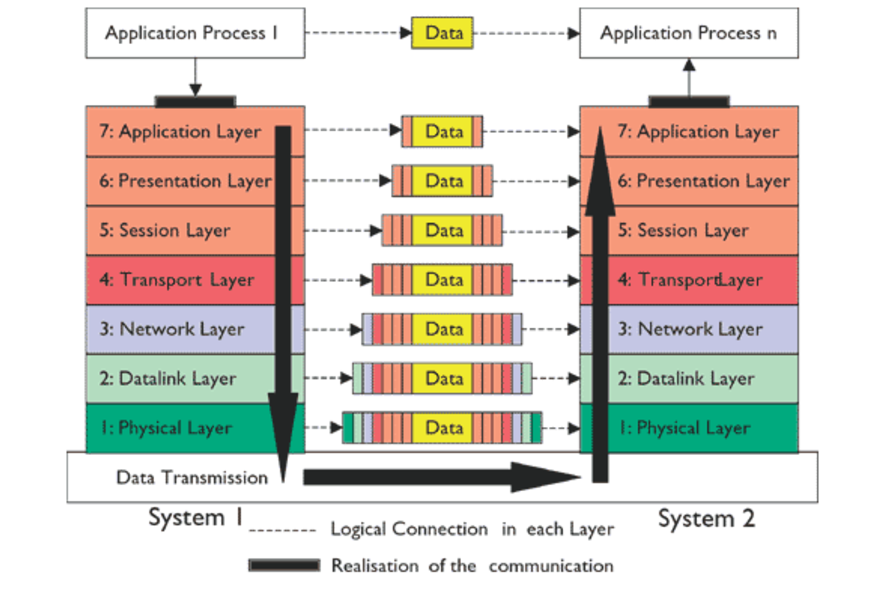
\includegraphics[angle=0, width=10cm]{./Figures/serial/modelOSI.pdf}
  \rule{35em}{0.5pt}
  \caption[osi]{Mod�le OSI}
  \label{fig:osi}
\end{figure}

Les couches qui sont n�cessaires � l'�tablissement d'une communication sont les couches 1 � 4. Les autres sont des couches li�es aux services et aux applications.

\begin{enumerate}
\item Couche physique: Traite les aspects �lectriques de la ligne s�rie
\item Couche paquet: Encapsule les donn�es avec des bits de contr�le e.g. pour la d�tection d'erreurs
\item Couche r�seau: Indique la destination (s'il y a plus que deux noeuds sur le r�seau)
\item Couche transport: D�coupe les donn�es en paquets et g�re la retransmission en cas d'erreurs
\end{enumerate}

\subsection{Pile protocolaire IP}
Le protocole IP (Internet Protocol) est simplifi� par rapport au mod�le OSI (fig. \ref{fig:tcpip}). Il ne contient que quatre couches ce qui parait plus simple mais en pratique n'est pas id�al car il groupe plusieurs fonctions dans une seule couche.

\begin{figure}[htb]
  \centering
  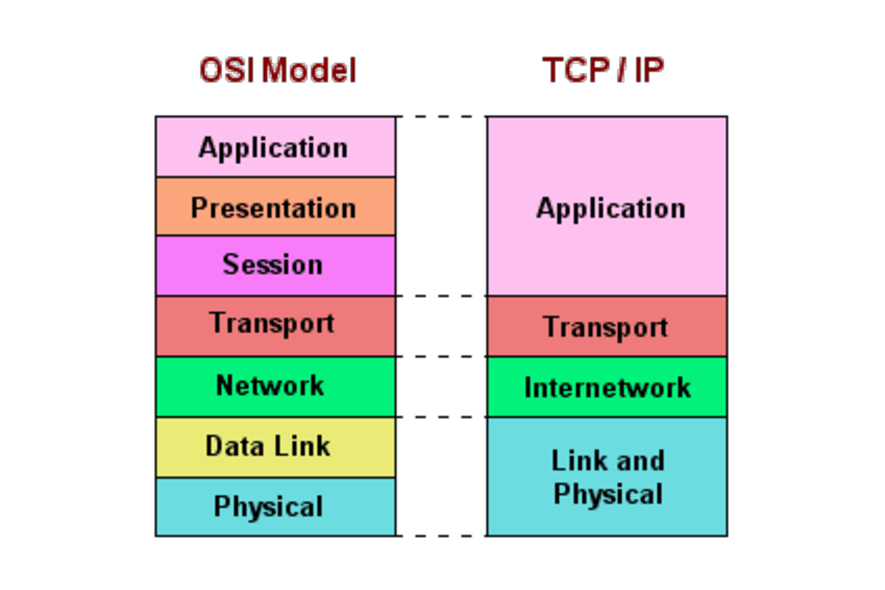
\includegraphics[angle=0, width=10cm]{./Figures/serial/tcpipstack.pdf}
  \rule{35em}{0.5pt}
  \caption[tcpip]{Comparaison des piles protocolaires}
  \label{fig:tcpip}
\end{figure}

\section{UART (Universal Asynchronous Receiver Transmitter)}

Les UART sont des s�rialiseurs/d�s�rialiseurs simples. Un UART permet d'impl�menter la couche 2 du mod�le OSI. L'UART est asynchrone ce qui veut dire qu'il ne propage pas de signal d'horloge de l'�metteur au r�cepteur. Il est n�anmoins ais� d'ajouter une ligne d'horloge pour rendre l'UART synchrone.

\begin{figure}[htb]
  \centering
  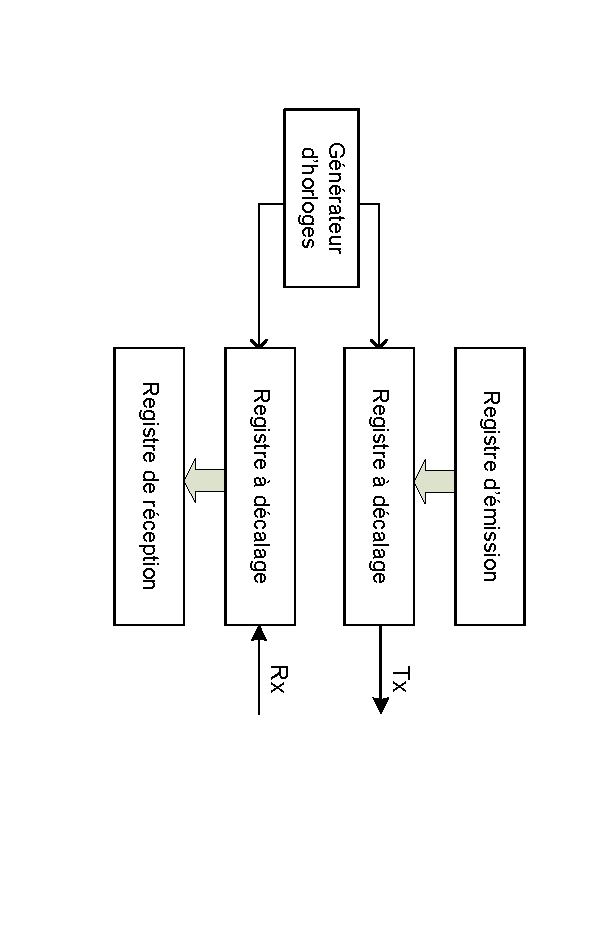
\includegraphics[angle=90, trim = 15mm 0mm 5mm 0mm, clip, width=13cm]{./Figures/serial/UART.pdf}
  \rule{35em}{0.5pt}
  \caption[uart]{Principe de fonctionnement d'une UART}
  \label{fig:tcpip}
\end{figure}

Au niveau mat�riel, l'UART est compos� de 4 registres dont deux � d�calage. Le g�n�rateur d'horloge donne la fr�quence de transmission ou vitesse de transmission. Du point de vue logiciel on acc�de � l'UART simplement en �crivant dans le registre d'�mission et en lisant le registre de r�ception.

\subsection{RS-232C}
Historiquement, les interfaces s�ries �taient tr�s simples d'un point de vue logiciel mais par contre plus compliqu�es d'un point de vue mat�riel. C'est le cas de l'interface RS-232C d�velopp�e en 1969.

La couche physique du RS-232C � n�anmoins �volu� depuis 1969, par contre la couche 2 est toujours la m�me. On peut r�aliser cette couche 2 avec un UART.

\section{Interface SPI}

Dix ans apr�s la RS-232C, Motorola invente l'interface SPI en 1979. C'est un changement radical, avec une communication synchrone entre les �metteurs et les r�cepteurs. Ce changement permet d'aller beaucoup plus vite dans la transmission.

\begin{figure}[htb]
  \centering
  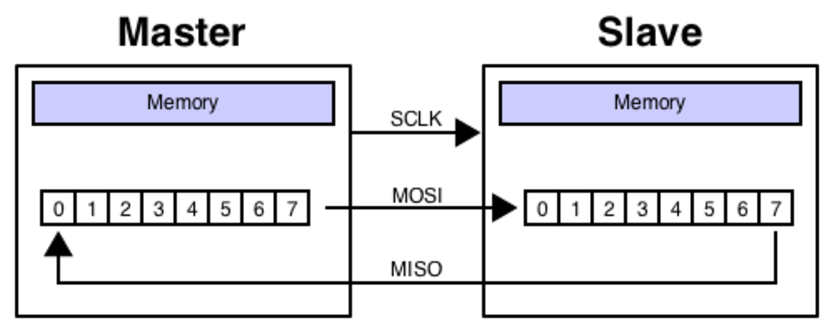
\includegraphics[width=12cm]{./Figures/serial/SPI_8-bit_circular_transfer.pdf}
  \rule{35em}{0.5pt}
  \caption[spi]{Principe de fonctionnement d'une interface SPI}
  \label{fig:tcpip}
\end{figure}

L'interface SPI utilise deux registres � d�calage boucl�s. Ceci permet de relire l'information transmise est ainsi v�rifier que ce qui a �t� transmis est bien correcte. Pour �crire ou lire, on utilise le m�me principe que pour l'UART, c-�-d �crire dans le registre d'�mission ou lire le registre de r�ception.

Il est possible de connecter plusieurs p�riph�riques sur une interface SPI � l'aide de signaux sortant d'un GPIO et allant sur une entr�e "chip-select" CS. Il faut juste s�lectionner le bon CS depuis le code.

\section{Interface I2C}

Trois ans apr�s la SPI, Philips invente l'interface I2C en 1982. Cette interface am�ne une innovation majeur qui est la r�alisation d'une couche 3 logicielle permettant d'adresser 256 noeuds. On peut donc relier tous les p�riph�riques d'une carte � l'aide d'une interface I2C. Ils sont connect�s sur deux lignes communes SDA et SCL:

\begin{figure}[htb]
  \centering
  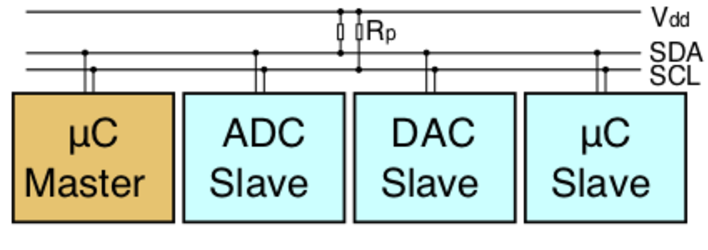
\includegraphics[width=10cm]{./Figures/serial/I2C.pdf}
  \rule{35em}{0.5pt}
  \caption[i2c]{Syst�me avec un bus I2C}
  \label{fig:tcpip}
\end{figure}

Les lignes, SDA et SCL, sont tir�es vers l'alimentation positive (Vdd) � l'aide de deux r�sistance pull-up. Elles doivent �tre dimensionn�es par rapport � la vitesse de transmission choisie. Pour s�lectionner un p�riph�rique en particulier, il faut connaitre son adresse I2C et la placer dans le registre d'adresse de l'interface.

\section{Interface USB}

L'interface s�rie la plus r�cente que l'on trouve dans les microcontr�leurs est l'USB (Universial Serial Bus) d�velopp�e en 1996. Cette interface � comme avantage majeur sur les autres l'utilisation d'une signalisation basse tension diff�rentielle LVDS (Low Voltage Differential Signal). Par contre, cette interface est purement point � point c-�-d qu'elle ne relie qu'un noeud � un autre. De ce fait, elle ne remplace pas les pr�c�dentes.

\begin{figure}[htb]
  \centering
  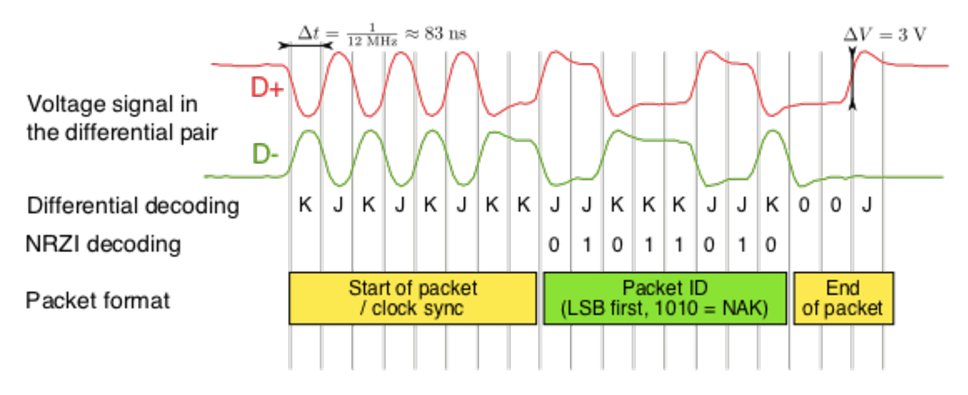
\includegraphics[width=14cm]{./Figures/serial/USB_signal_example.pdf}
  \rule{35em}{0.5pt}
  \caption[usb]{Exemple de signal USB}
  \label{fig:tcpip}
\end{figure}

L'interface USB est synchrone mais ne poss�de pas de ligne de clock. L'horloge est retrouv�e � la r�ception gr�ce � une s�quence d'entrainement de 8 bits. Une fois l'horloge synchronis�e un packet ID (PID) est envoy� pour donner le type de message envoy�. Si le PID indique des donn�es alors elles sont transmises. Finalement le paquet est termin� par une s�quence "End of Packet" de trois bits.

D'un point de vue logiciel, l'interface USB s'acc�de gr�ce � un HAL ou par un pilote si il y a un syst�me d'exploitation.

\section{Comparaisons et choix d'une interface}

\begin{table}[!htbp]
\begin{center}
{\fontfamily{phv}\selectfont
\begin{tabular}{|c|c|c|c|c|c|}
\hline 
Interface & Noeuds & Vitesse & Async/Sync & Duplex & Utilisation\\
\hline  
\hline 
RS-232C & 1 & 115kHz & A & Full & Terminal\\
\hline 
SPI & 1 � 5 & 100MHz & S & Full & Donn�es\\
\hline
I2C & 256 & 1MHz & S & Half & Configuration\\
\hline
USB 2.0 & 1 & 480MHz & S & Half & External\\
\hline
\end{tabular}
}
\end{center}
\caption{Comparaisons entre les diff�rentes interfaces s�ries \label{serial}}
\end{table}

\section{Cas du MSP430}

Le MSP430 dispose de toutes les interfaces discut�es pr�c�demment. Il s'agit donc de d�terminer les registres de configuration propres � chaque interface puis de les param�trer correctement.

Exemple de configuration d'une interface s�rie asynchrone, style RS-232C:

\lstset{style=customc}
\begin{lstlisting}
UCA0CTL0 |= UCPEN | UCPAR;	//parity enabled, even, one stop(default), 8-bit (default), async (default)
UCA0CTL1 |= UCSSEL_2;		//SMCLK
UCA0BR0 = 0x09;				//115200 bauds selon table du fabriquant
UCA0BR1 = 0x00;
UCA0MCTL = 0x02;			//115200 bauds selon table du fabriquant		
 
UCA0IE |= UCRXIE | UCTXIE;	//Interrupt enable
	
P2DIR |= 0x01;				//P2.0 vers sortie 	 
 
#pragma vector=USCI_A0_VECTOR
__interrupt void USCI_A0_ISR(void)
{
  switch(__even_in_range(UCA0IV,4))
  {
    case  0: 	break;
    case  2: 	while (!(UCA0IFG & UCTXIFG));
				UCA0TXBUF = UCA0RXBUF;
				break;
    case  4: 	P2OUT ^= 0x01;		// toggle P2.0 avec exclusive-OR 
				break;
    default: 	break;
  }
}
\end{lstlisting}

L'interaction avec les registres de r�ception ou d'�mission est effectu�e par interruption dans ce cas ci. Le vecteur USCI\_A0\_VECTOR contient plusieurs sources d'interruptions possibles c'est pourquoi il faut les s�lectionner � l'aide d'un switch case. Le "case 2" correspond � une r�ception et le "case 4" � une �mission. Lors d'une r�ception on test si l'�mission n'est pas active puis on copie le message re�u sur la sortie. C'est un relai qui allume une LED lorsque le message a �t� relay�.

\chapter{\textsc{AD et DA}}

Les Convertisseurs Analogique-Num�rique (ADC pour \it Analog to Digital Converter \rm) et Num�rique-Analogique (DAC pour \it Digital to Analog Converter \rm) sont des �l�ments importants de toute cha�ne d'acquisition de donn�e.\\
En effet, les op�rations complexes de traitement de signal sont aujourd'hui ex�cut�es par des circuits num�riques, dont les microcontr�leurs font partie. Pour �tre trait�s par un microcontr�leur, les signaux analogiques doivent donc �tre convertis en nombres.\\
La figure \ref{fig:Acq_Chain} illustre une cha�ne typique d'acquisition de donn�e.

\begin{figure}[htb]
  \centering
  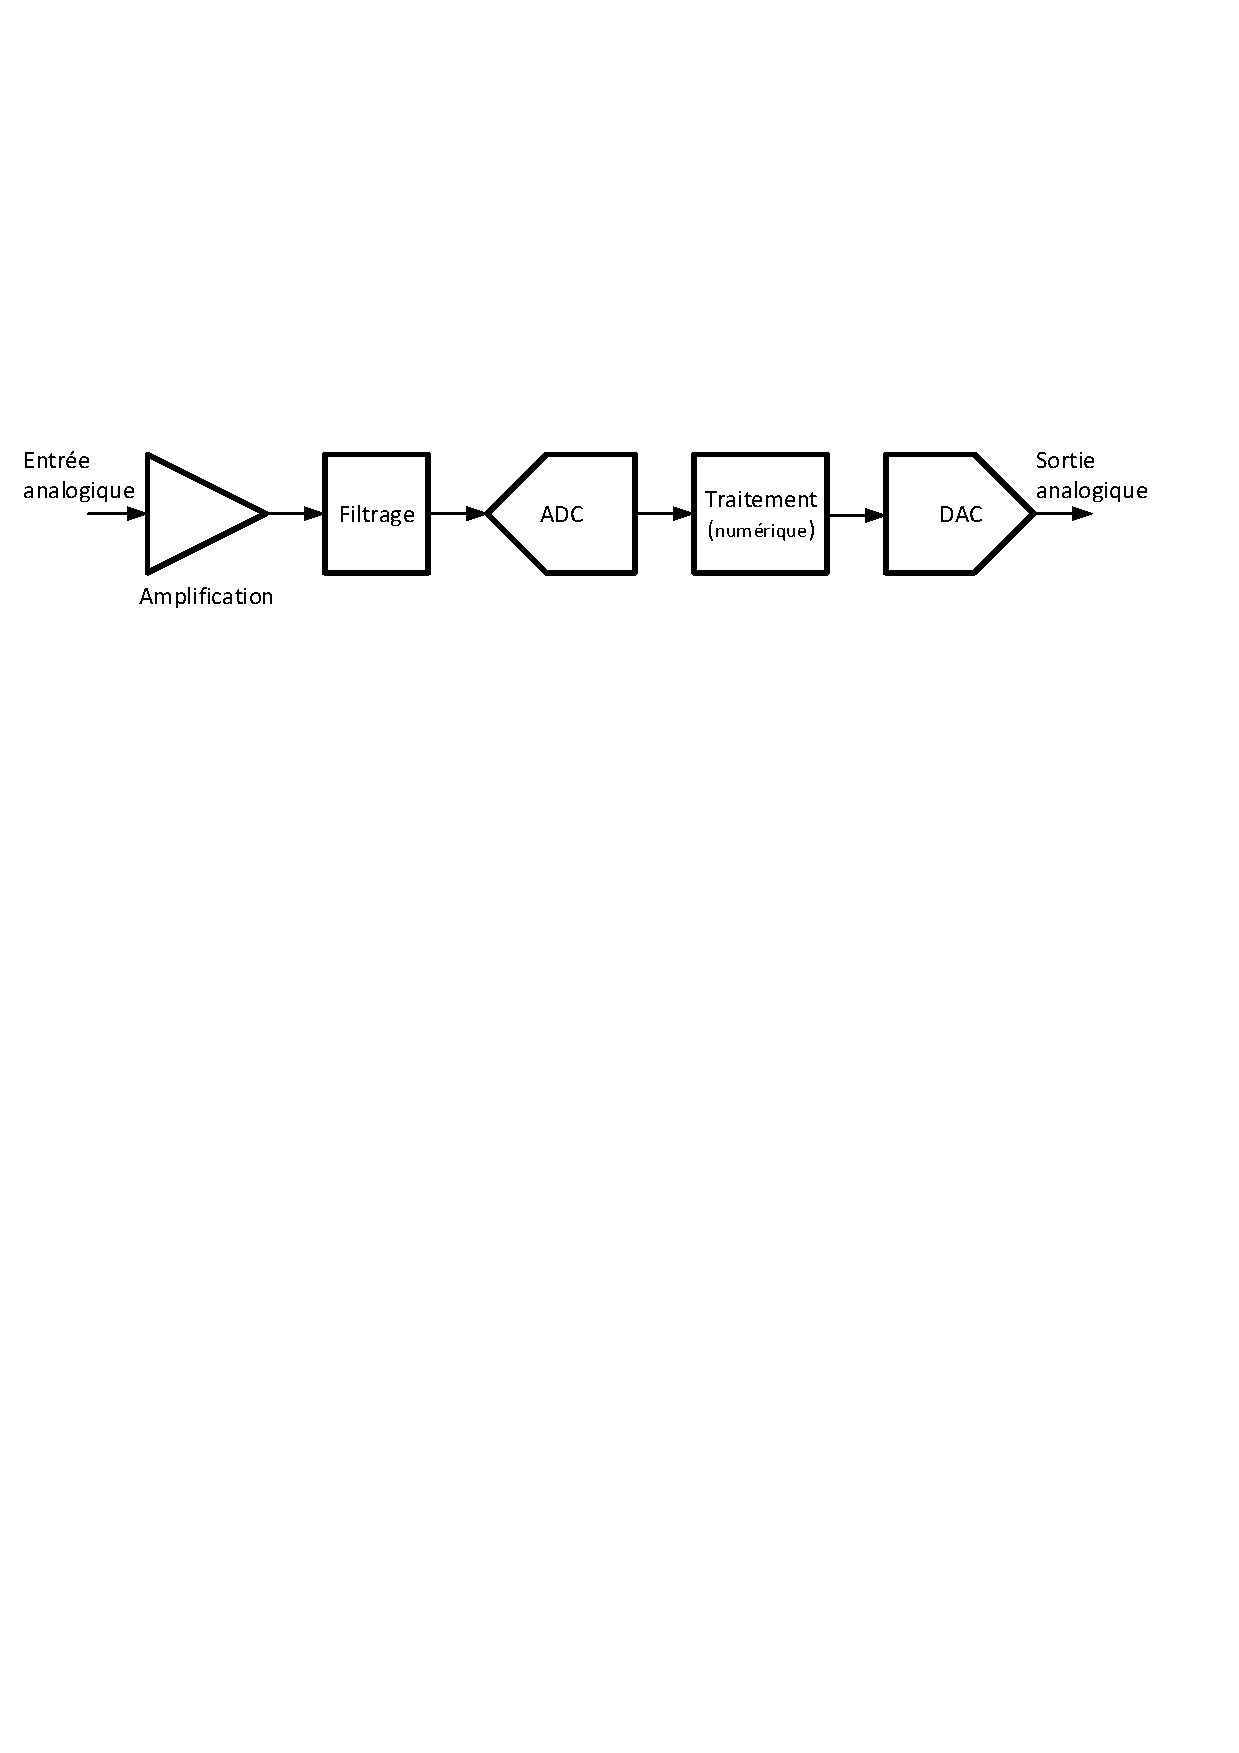
\includegraphics [angle=0, width=14cm]{./Figures/Chap11_ADC/Acq_Chain.pdf}
  \rule{35em}{0.5pt}
  \caption{Cha�ne d'acquisition et traitement de signal}
  \label{fig:Acq_Chain}
\end{figure}

\section{Convertisseur AD}
L'ADC est un circuit dont la fonction est de convertir une grandeur physique $V_{in}$ - en g�n�ral une tension, parfois un courant - en un nombre N repr�sent� sur plusieurs bits, "proportionnel" � cette grandeur physique.
Le terme proportionnel est abusif dans la mesure o� la fonction de transfert $N = f(V_{in})$ est une fonction en escalier, comme illustr� � la figure \ref{fig:ADC_Fonction}.

\begin{figure}[htb]
  \centering
  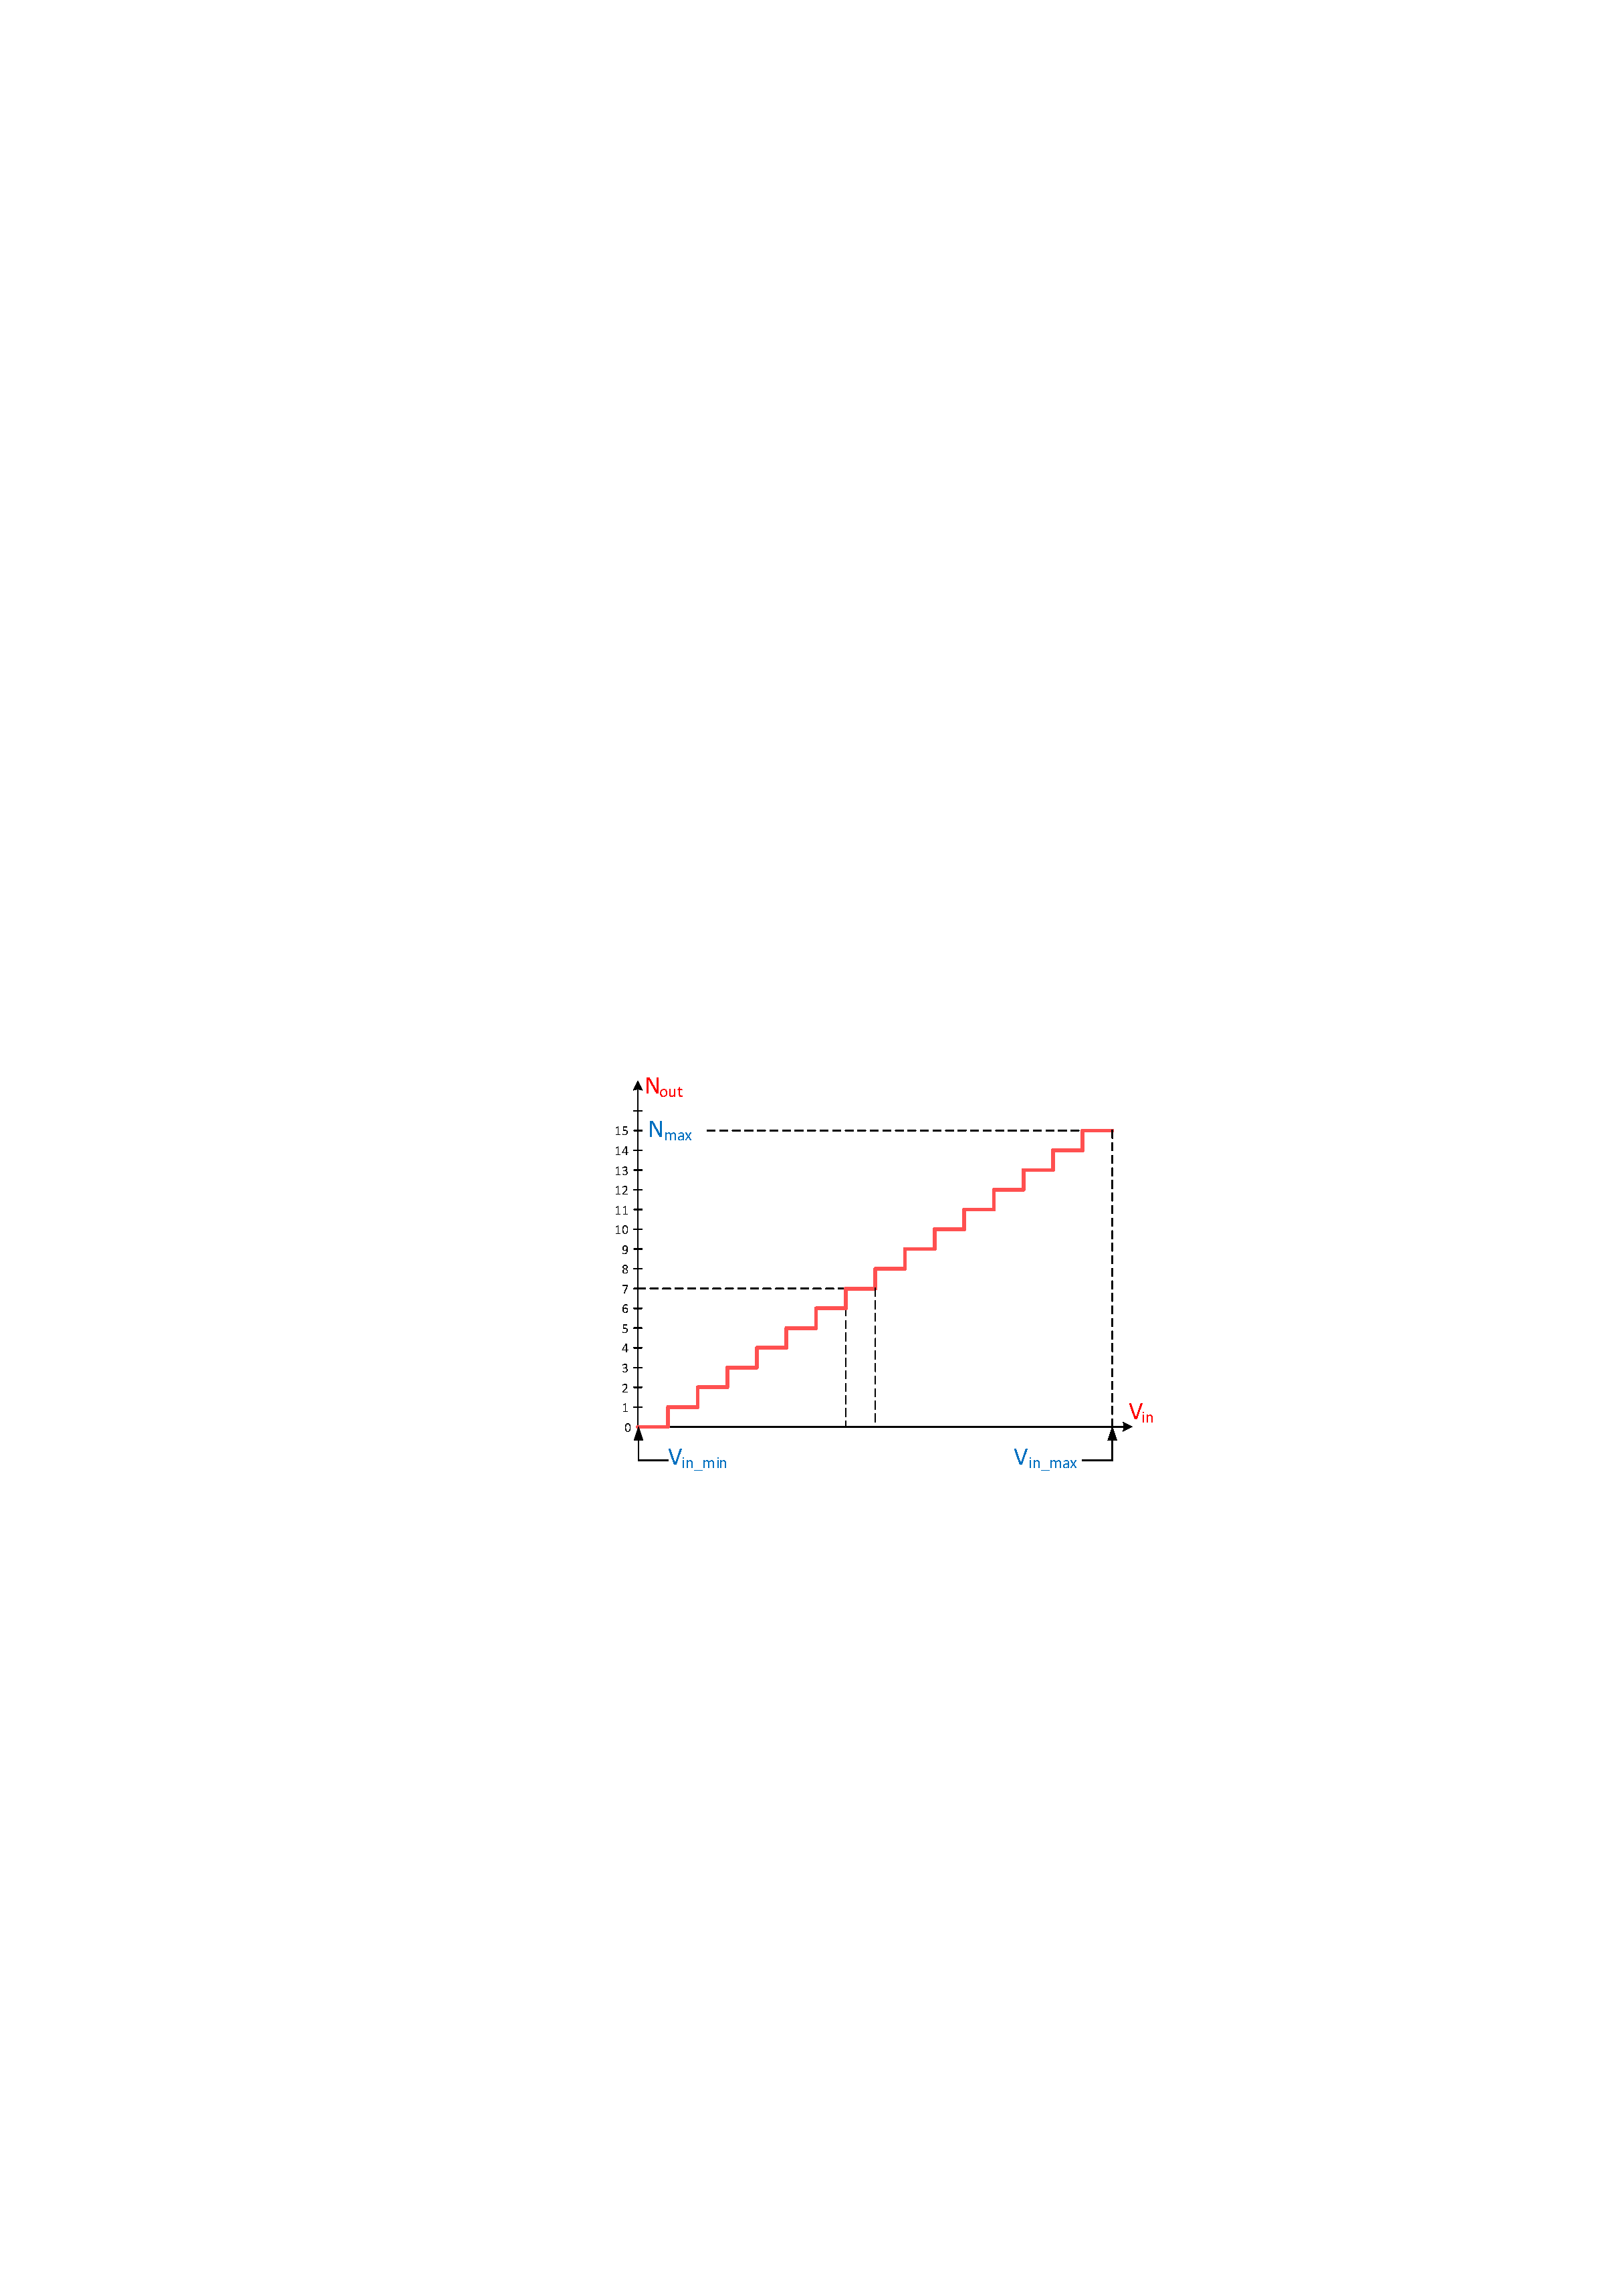
\includegraphics [angle=0, width=10cm]{./Figures/Chap11_ADC/ADC_Fonction.pdf}
  \rule{35em}{0.5pt}
  \caption{Fonction de transfert d'un ADC id�al 4-bits}
  \label{fig:ADC_Fonction}
\end{figure}

Les caract�ristiques importantes de cette fonction de transfert sont:
\begin{itemize}[label=\textbullet,font=\small]
\item l'intervalle des tensions d'entr�e $[V_{in\_min}, V_{in\_max}$]
\item la r�solution, �gale � $log_{2}(N_{max})$
\item les imperfections qui l'entachent, et qui sont:
\begin{itemize}[label=\textbullet,font=\small]
\item offset
\item erreur de gain
\item "non lin�arit�" de la fonction
\end{itemize}
\end{itemize}

Il existe plusieurs m�thodes pour convertir une grandeur physique en un nombre. Elles se diff�rencient principalement par la r�solution atteignable et la rapidit� du processus de conversion, et aussi par leur complexit�.\\
Dans les microcontr�leurs, le convertisseur AD le plus souvent rencontr� est le convertisseur � approximations successives, dont l'avantage est d'offrir un bon compromis entre r�solution et rapidit�, pour une consommation de courant tr�s faible.

\section{Convertisseur � approximations successives}

Ce type de convertisseur utilise un processus de dichotomie pour traduire progressivement une tension analogique en un nombre. Le temps de conversion est fonction du nombre de bits souhait�s.\\
Le principe est illustr� � la figure \ref{fig:ADC_SAR_Diagram}.

\begin{figure}[htb]
  \centering
  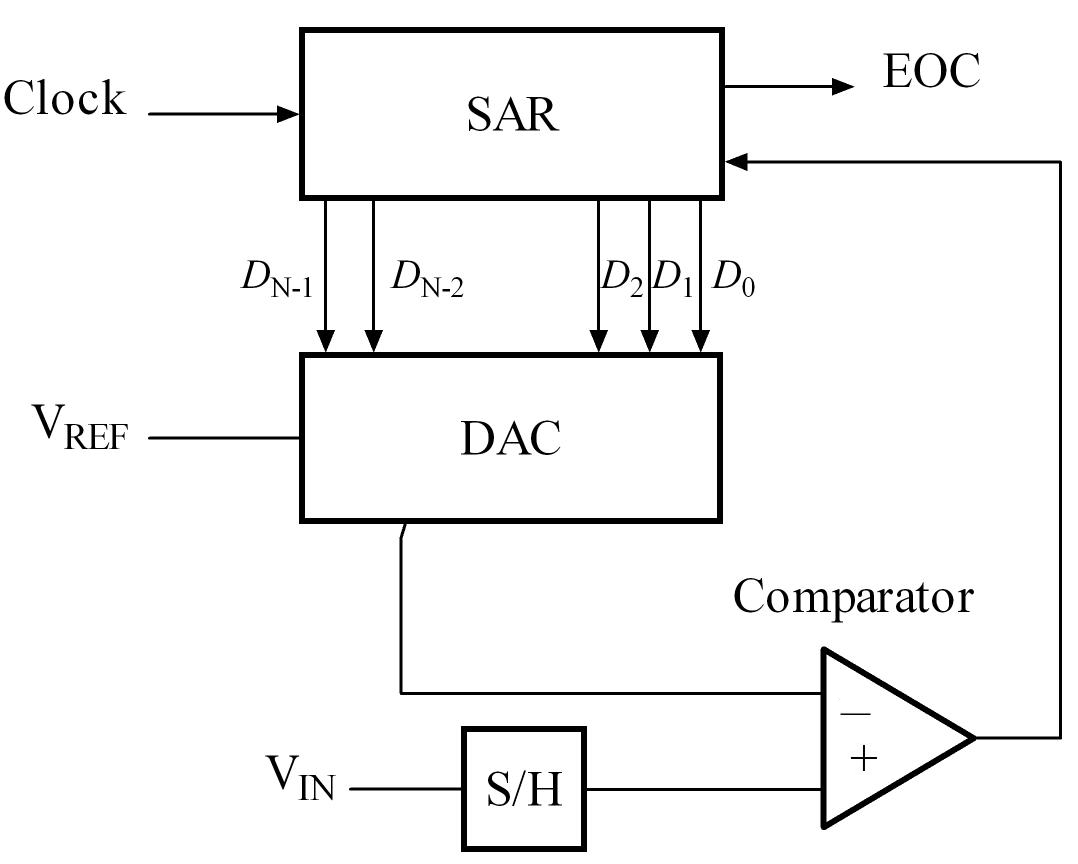
\includegraphics [angle=0, width=10cm]{./Figures/Chap11_ADC/SA_ADC_block_diagram.png}
  \rule{35em}{0.5pt}
  \caption{Principe du convertisseur � approximations successives}
  \label{fig:ADC_SAR_Diagram}
\end{figure}

Un s�quenceur (g�n�ralement nomm� SAR pour \it Successive Approximation Register\rm), coupl� � un convertisseur Digital-Analogique (DAC) g�n�re une tension analogique, qui est compar�e au signal � convertir.
Le r�sultat de cette comparaison est alors introduit dans le SAR, qui va le prendre en compte, pour la suite du processus de dichotomie, jusqu'� compl�tion. La figure \ref{fig:ADC_SAR} illustre la chronologie du processus de conversion, dans le cas d'un ADC 4-bits.\\
Dans cet exemple, le DAC est capable de g�n�rer 16 tensions not�es $x.FS$ (FS signifie \it Full Scale\rm), avec $0 \leqslant x \leqslant 15$. Les valeurs minimale et maximale de ces tensions sont appel�es \it tensions de r�f�rence\rm.\\
Le test du MSB d�termine si $V_{in}$ est sup�rieur ou inf�rieur � $\scriptstyle {}^1\!/\!_2.FS$. Dans l'exemple, d�s lors que $V_{in} \leqslant \scriptstyle {}^1\!/\!_2.FS$, le MSB vaut 1. Pour tester le bit de poids inf�rieur (MSB-1), le s�quenceur commande le DAC pour qu'il g�n�re $\scriptstyle {}^3\!/\!_4.FS$. Cette fois,  $V_{in} \geqslant \scriptstyle {}^3\!/\!_4.FS$, donc (MSB-1) = 0; ceci signifie qu'il ne fallait pas ajouter $\scriptstyle {}^1\!/\!_4.FS$ � 
$\scriptstyle {}^1\!/\!_2.FS$ mais $\scriptstyle {}^1\!/\!_8.FS$.\\
Le processus continue ainsi jusqu'� l'obtention du LSB, au rythme d'un bit par �tape.

\begin{figure}[htb]
  \centering
  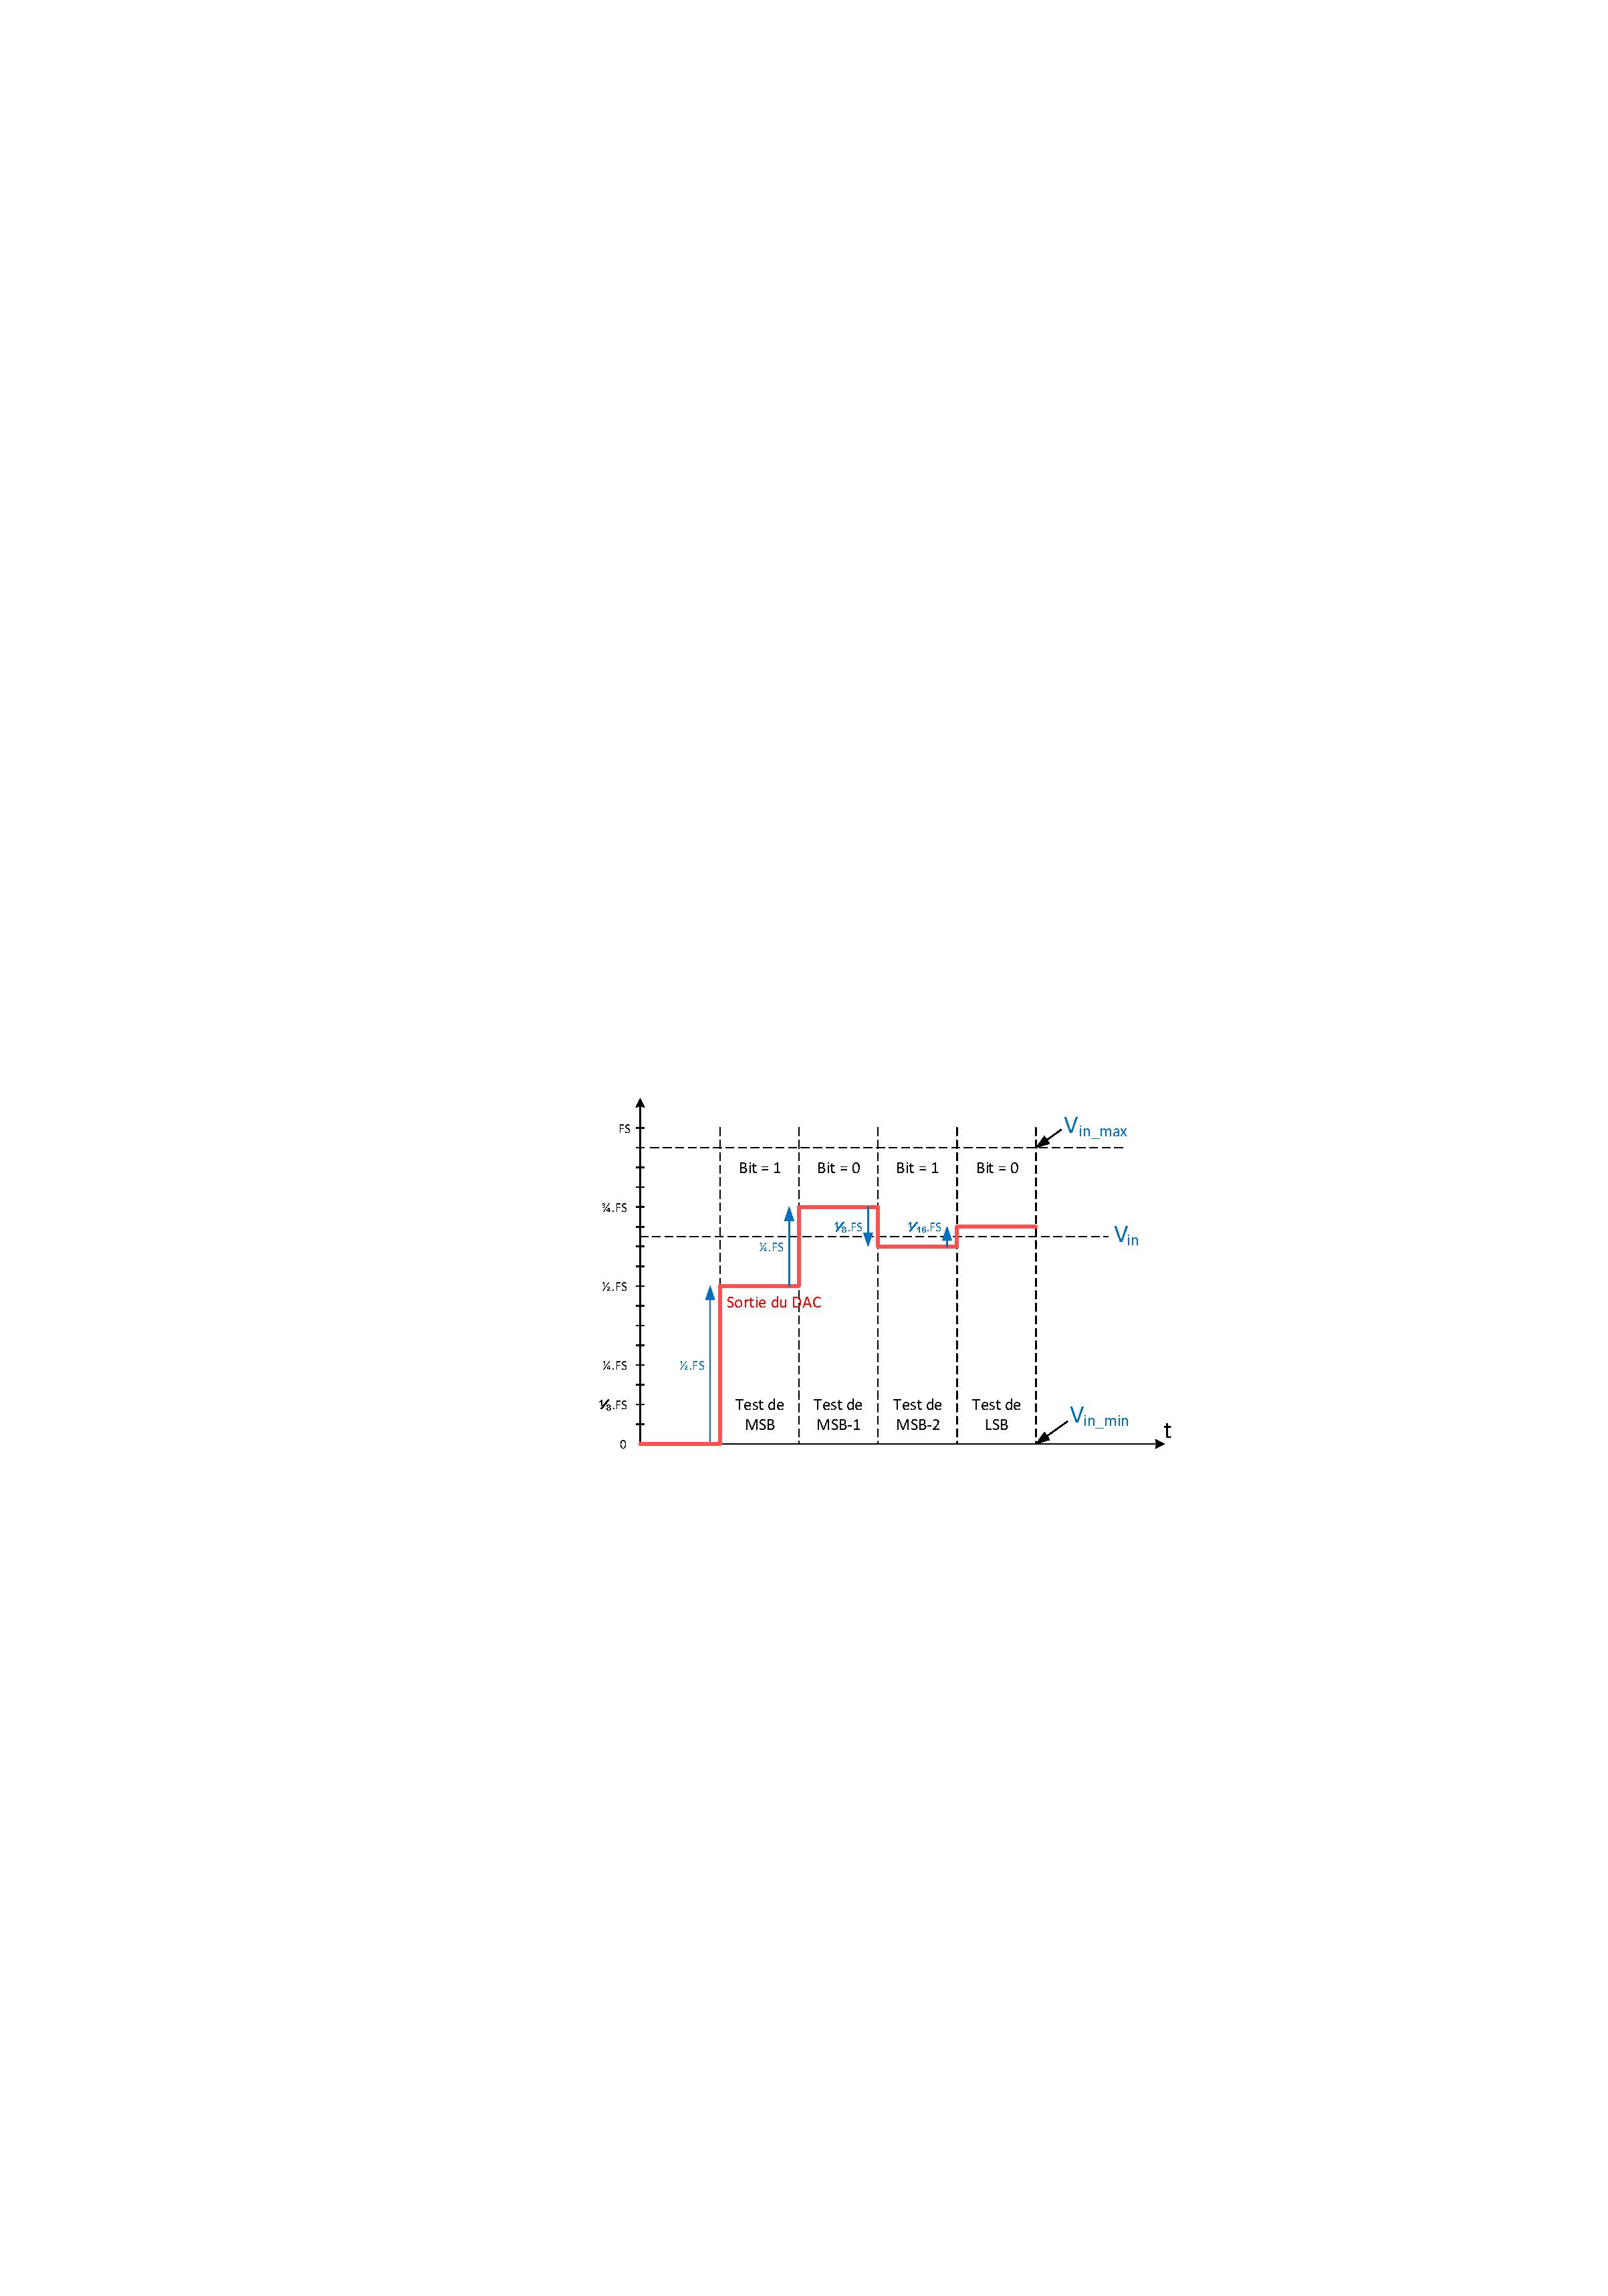
\includegraphics [angle=0, width=13cm]{./Figures/Chap11_ADC/ADC_SAR.pdf}
  \rule{35em}{0.5pt}
  \caption{Etapes de conversion d'un ADC 4-bits � approximations successives}
  \label{fig:ADC_SAR}
\end{figure}

Le convertisseur r�alise donc sa conversion en positionnant en premier le bit de poids fort (MSB) et en descendant progressivement jusqu'au LSB.
Ces convertisseurs ont des r�solutions d'une douzaine de bits environ, mais peuvent atteindre 16 bits au moyen de technologies sp�ciales.\\

Il est important de noter que la tension d'entr�e doit �tre m�moris�e pendant toute la dur�e du processus de conversion. Ceci est effectu� au moyen d'un circuit auxiliaire appel� "Echantillonneur-Bloqueur" (\it Sample and Hold\rm). Le terme "Echantillonneur" fait r�f�rence � l'instant auquel la tension est saisie; "Bloqueur" fait r�f�rence � sa m�morisation. 

Le convertisseur DAC peut �tre construit au moyen de:
\begin{itemize}[label=\textbullet,font=\small]
\item un diviseur de tension r�sistif coupl� � des interrupteurs
\item un diviseur de courant de type R-2R
\item un diviseur de tension � capacit�s pond�r�es
\end{itemize}
Le d�tail de ces circuits sort du cadre de ce cours.

\section{Cas du MSP430}
Les microcontr�leurs MSP430 peuvent contenir plusieurs types de convertisseurs AD:
\begin{itemize}[label=\textbullet,font=\small]
\item AD 10-bits � approximations successives
\item AD 12-bits � approximations successives
\item AD 16-bits Sigma-Delta
\end{itemize}

\subsection{Cas du MSP430F5529}
Ce microcontr�leur contient un convertisseur AD 12 bits � approximations successives avec les caract�ristiques suivantes.
\begin{itemize}[label=\textbullet,font=\small]
\item Plus de 200 kSPS : 200'000 �chantillons par seconde
\item Echantillonneur-Bloqueur avec p�riode programmable, contr�l�e par logiciel ou par timers
\item Lancement des conversions par logiciel ou par timers
\item R�f�rence de tension interne s�lectionnable par logiciel (1.5 V, 2.0 V, ou 2.5 V)
\item R�f�rence interne ou externe
\item Jusqu'� 12 canaux d?entr�e configurables individuellement
\item Canaux d'entr�e pour capteur de temp�rature interne, AVCC, et r�f�rences externes
\item Registres de stockage de 16 r�sultats de conversion
\end{itemize}

\subsection{Sch�ma de l'ADC 12-bits}
La figure \ref{fig:ADC_Schema} repr�sente le sch�ma complet du p�riph�rique ADC12, l'ADC 12-bits pr�sent dans le MSP430F5529. 

\begin{figure}[H]
  \centering
  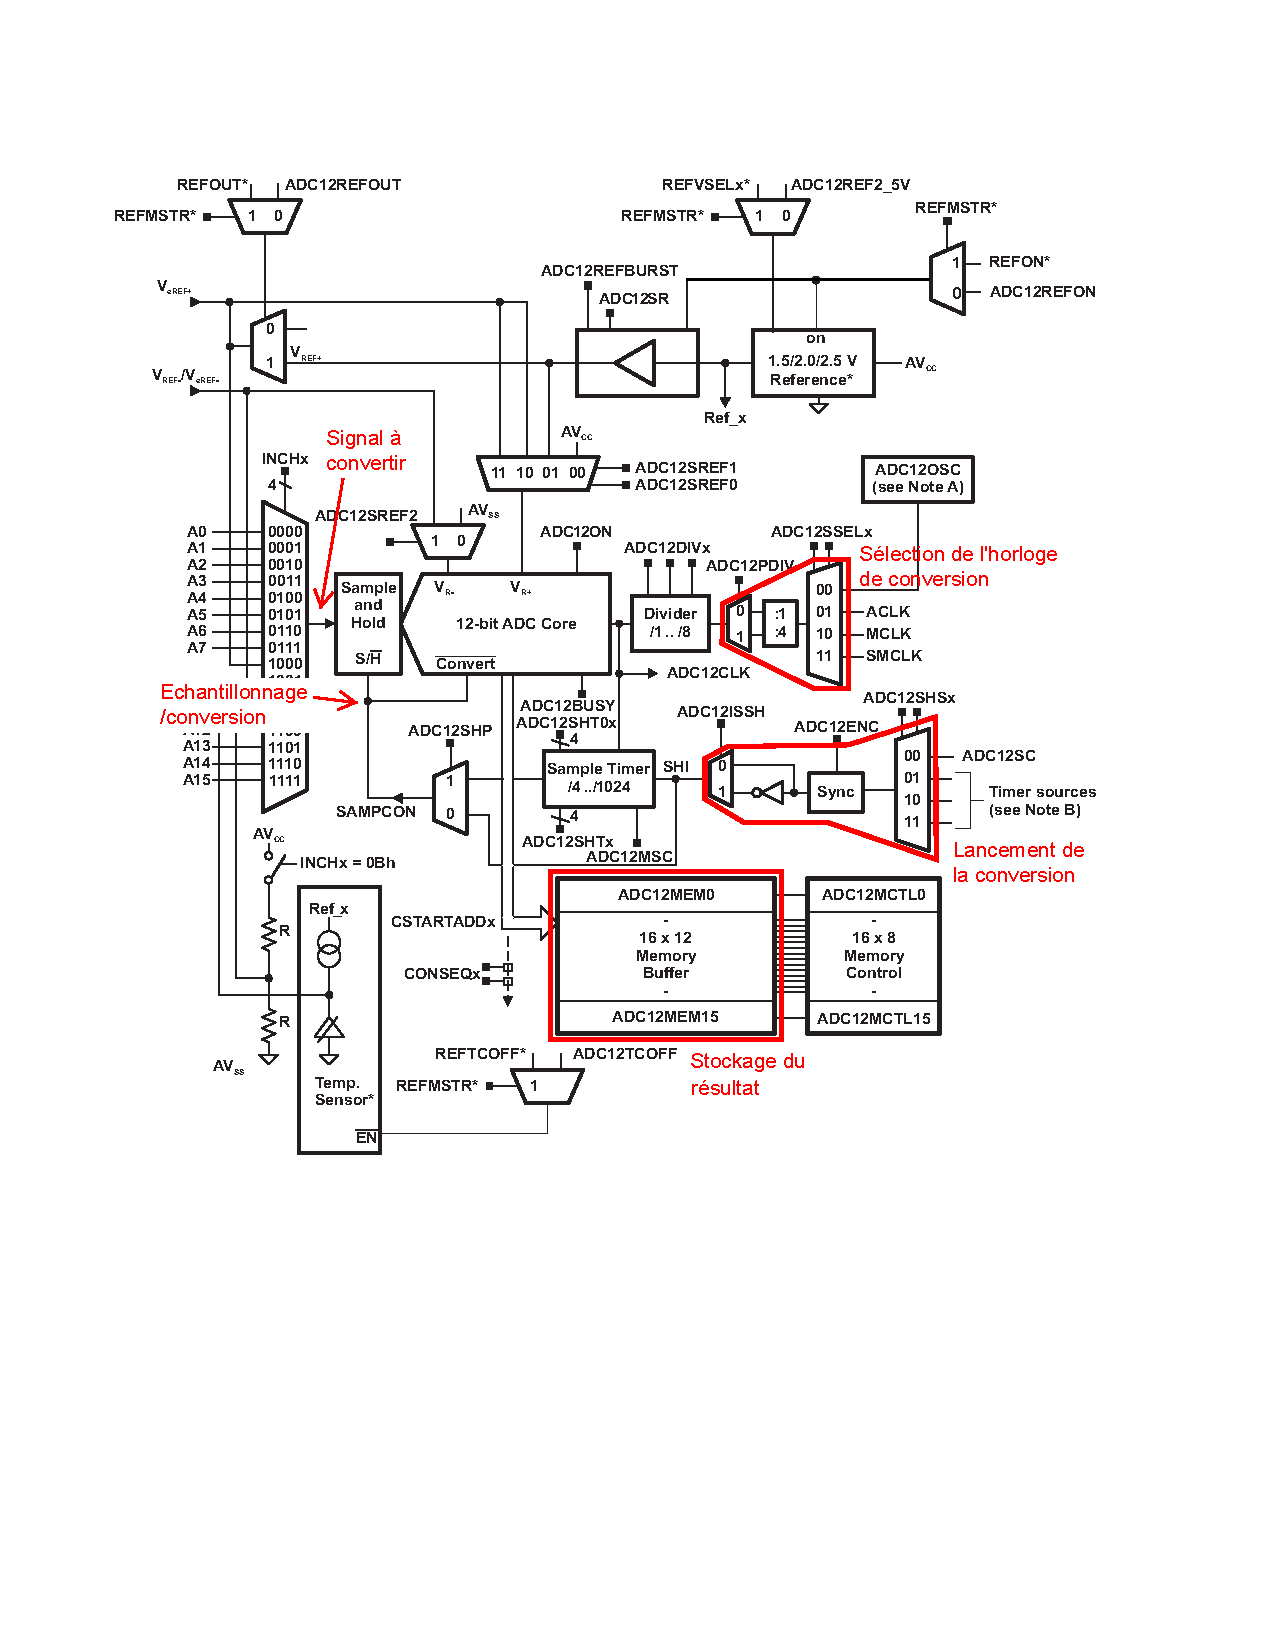
\includegraphics [angle=0, width=16cm]{./Figures/Chap11_ADC/ADC_Schema.pdf}
  \rule{35em}{0.5pt}
  \caption{Sch�ma du convertisseur ADC12 dans le MSP430F5529}
  \label{fig:ADC_Schema}
\end{figure}

On y trouve:
\begin{itemize}[label=\textbullet,font=\small]
\item le coeur de l'ADC, avec l'�chantillonneur-bloqueur, au centre
\item le bloc de s�lection des r�f�rences de tension
\item le bloc de s�lection de l'horloge de conversion, qui d�finit le rythme auquel les bits du r�sultat sont obtenus
\item le bloc de lancement d'une conversion. Il est possible de lancer automatiquement des conversions
\item une m�moire pouvant contenir les r�sultats de 16 conversions
\item � gauche, le circuit de s�lection du signal � convertir
\end{itemize}

Comme on l'a d�j� vu avec d'autres p�riph�riques, les r�glages du convertisseur ADC12 se font par le logiciel, en positionnant les champs logiques apparaissant sur le sch�ma, qui sont accessibles dans des registres de contr�le.

\pagebreak
\subsection{Echantillonnage et conversion}
Le processus de conversion commence par l'�chantillonnage du signal d'entr�e, puis continue avec la conversion par approximations successives. Le processus est lanc� sur le flanc montant du signal SHI, comme indiqu� � la figure \ref{fig:ADC12SHP1}.

\begin{figure}[H]
  \centering
  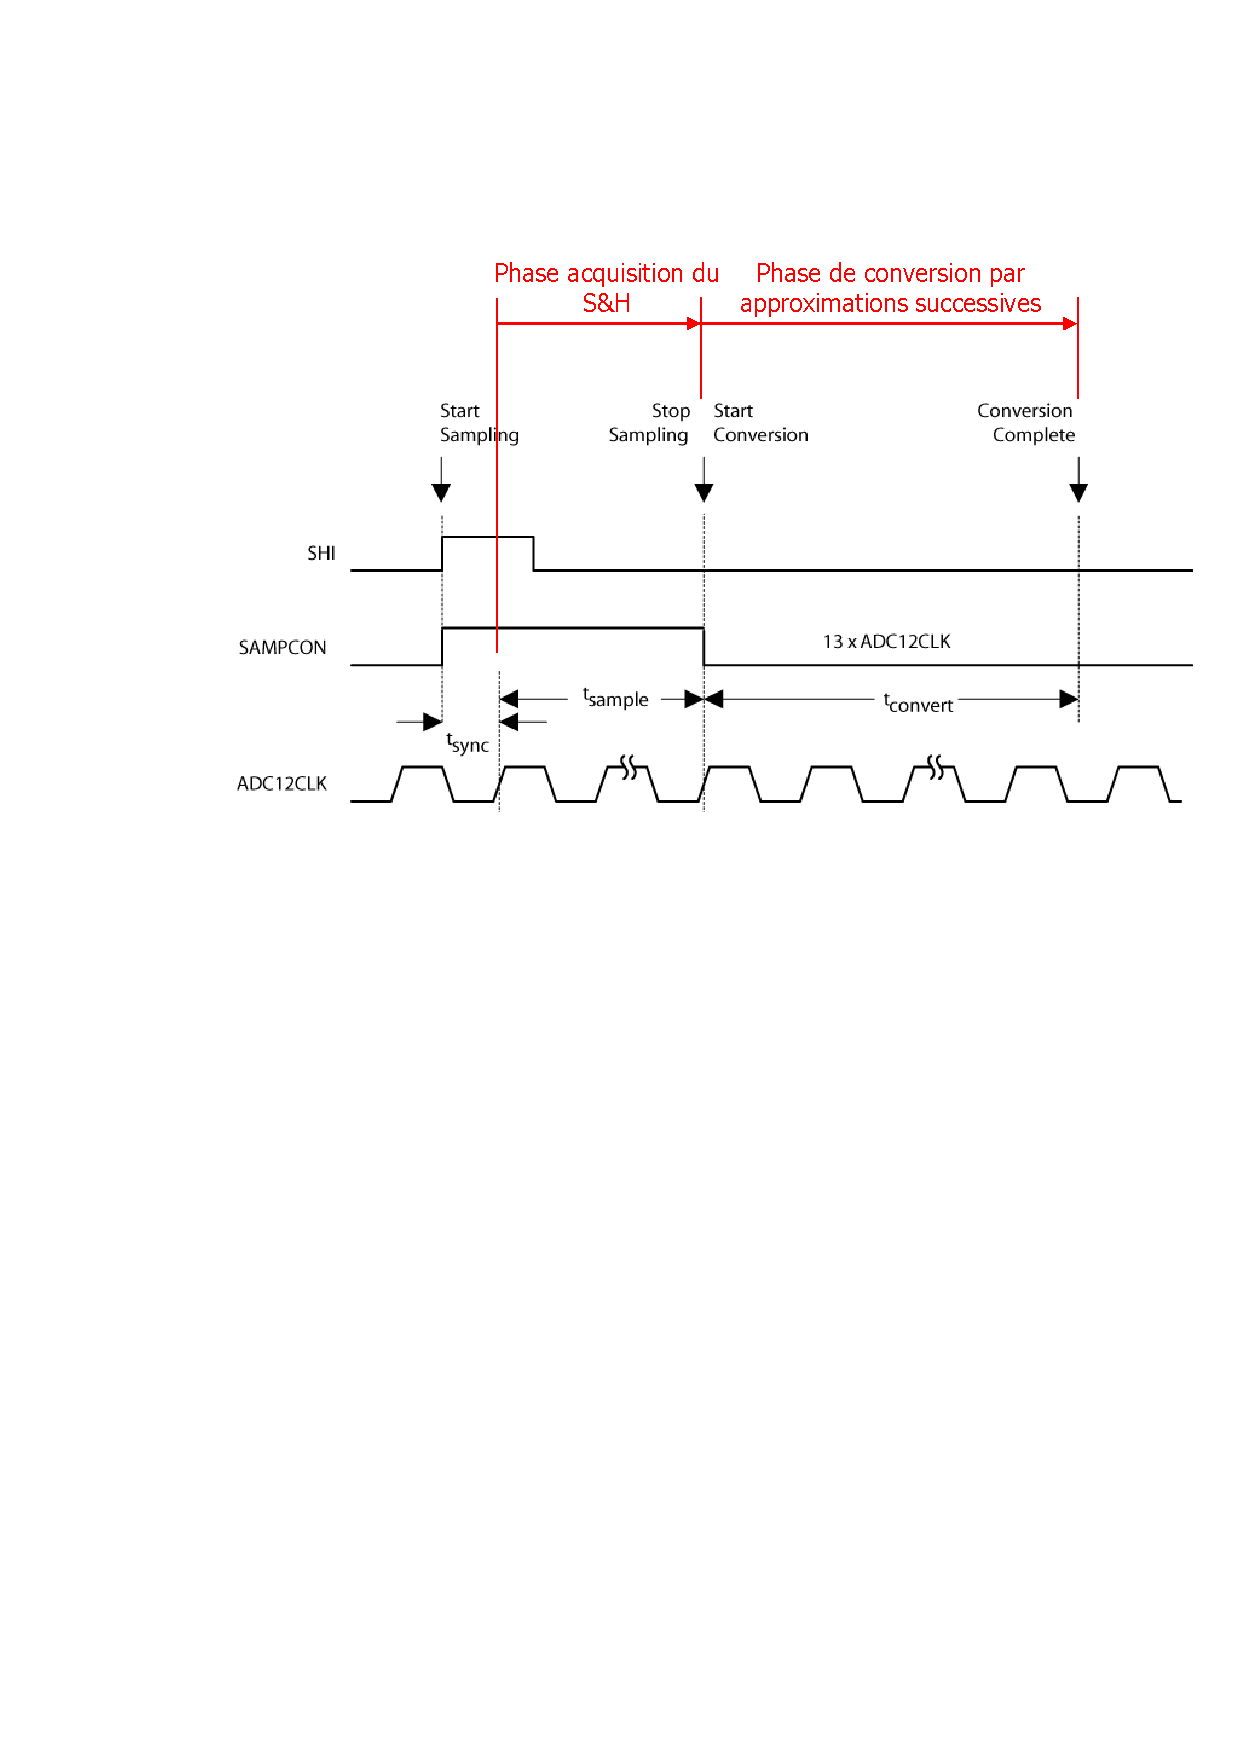
\includegraphics [angle=0, width=14cm]{./Figures/Chap11_ADC/ADC12SHP1.pdf}
  \rule{35em}{0.5pt}
  \caption{Chronogramme du processus d'�chantillonnage et conversion (ADC12SHP = 1)}
  \label{fig:ADC12SHP1}
\end{figure}

Le signal SAMPCON (\it Sampling Control\rm) joue un r�le particulier car son flanc montant d�termine le d�but de la saisie du signal d'entr�e, qui dure tant que $SAMPCON = 1$. La conversion � proprement parler d�marre au flanc descendant de  SAMPCON et dure 13 p�riodes du signal ADC12CLK pour une conversion sur 12 bits.
La dur�e du signal SAMPCON doit �tre r�glable pour pouvoir ajuster le temps d'�chantillonnage � la r�sistance interne de la source d'o� provient $V_{in}$. En effet, l'entr�e de l'�chantillonneur-bloqueur (le \it Sample and Hold\rm) est une capacit�; sa charge est soumise � une constante de temps qui d�pend de la r�sistance de la source.\\

\subsection{S�lection de l'horloge de conversion}
L'horloge de conversion ADC12CLK rythme le processus de conversion par approximations successives. Elle d�termine donc le temps allou� au calcul de chaque bit, du MSB au LSB.\\

Lorsque l'utilisateur souhaite se simplifier la vie (ADC12SHP = 1), elle d�termine aussi la dur�e de l'�chantillonnage, via un timer interne � l'ADC\footnote{La dur�e d'�chantillonnage peut aussi �tre contr�l�e par le programme. Dans ce cas (ADC12SHP = 0) le signal SHI contr�le directement la dur�e d'�chantillonnage et la conversion. SHI est alors g�n�r� par le programme ou par un des timers � usage g�n�ral}. Ce timer, not� \it Sample Timer\rm  sur la figure \ref{fig:ADC_Schema} peut g�n�rer une dur�e d'�chantillonnage comprise entre 4 et 1024 cycles du signal ADC12CLK.

Les sources d'horloge usuelles (ACLK, SMCLK et MCLK) s�euvent �tre utilis�es. Par d�faut, un autre signal est disponible, not� ADC12OSC, et dont la fr�quence est d'environ 5 MHz.

\subsection{Lancement d'une conversion}
Plusieurs m�thodes sont envisageables:
\begin{itemize}[label=\textbullet,font=\small]
\item lancement par logiciel, en activant le bit ADC12SC (\it Start Conversion\rm)
\item lancement automatique par un timer
\end{itemize}

\subsection{S�lection des r�f�rences de tension}
Les r�f�rences de tension d�terminent l'intervalle dans lequel la tension � convertir doit se trouver. La borne inf�rieure peut �tre �gale � GND, mais pas n�cessairement. Par contre, la borne sup�rieure est toujours inf�rieure � la tension d'alimentation VCC. La raison est que les circuits internes au convertisseur ont besoin d'une marge entre $V_{REF_Sup}$ et VCC pour pouvoir fonctionner correctement.

\subsection{Stockage des r�sultats}
Lorsqu'une conversion est termin�e, l'ADC peut �mettre une requ�te d'interruption. Toutefois, dans de nombreuses applications, il est n�cessaire de convertir plusieurs tensions diff�rentes. Les raisons peuvent �tre:
\begin{itemize}[label=\textbullet,font=\small]
\item les signaux g�n�r�s par plusieurs capteurs, et connect�es sur l'ADC via ses diff�rentes entr�es (A0 � A15) doivent �tre convertis en nombres;
\item plusieurs valeurs successives d'une m�me tension doivent �tre converties, pour pouvoir calculer une moyenne ou y appliquer une fonction de filtrage num�rique;
\item on ne souhaite pas surcharger le CPU avec des interruptions trop fr�quentes;
etc...
\end{itemize}

Pour r�soudre ce genre de situation, l'ADC dispose d'une m�moire pouvant contenir jusqu'� 16 r�sultats de conversion. Il est possible de d�finir des s�quences de conversion, et de faire en sorte qu'une interruption ne soit �mise qu'� la fin de la s�quence.\\
Chacun des 16 registres de stockage, not�s ADC12MEMx est associ� � un registre de contr�le not� ADC12MCTLx (x = 0..15).

\begin{figure}[H]
  \centering
  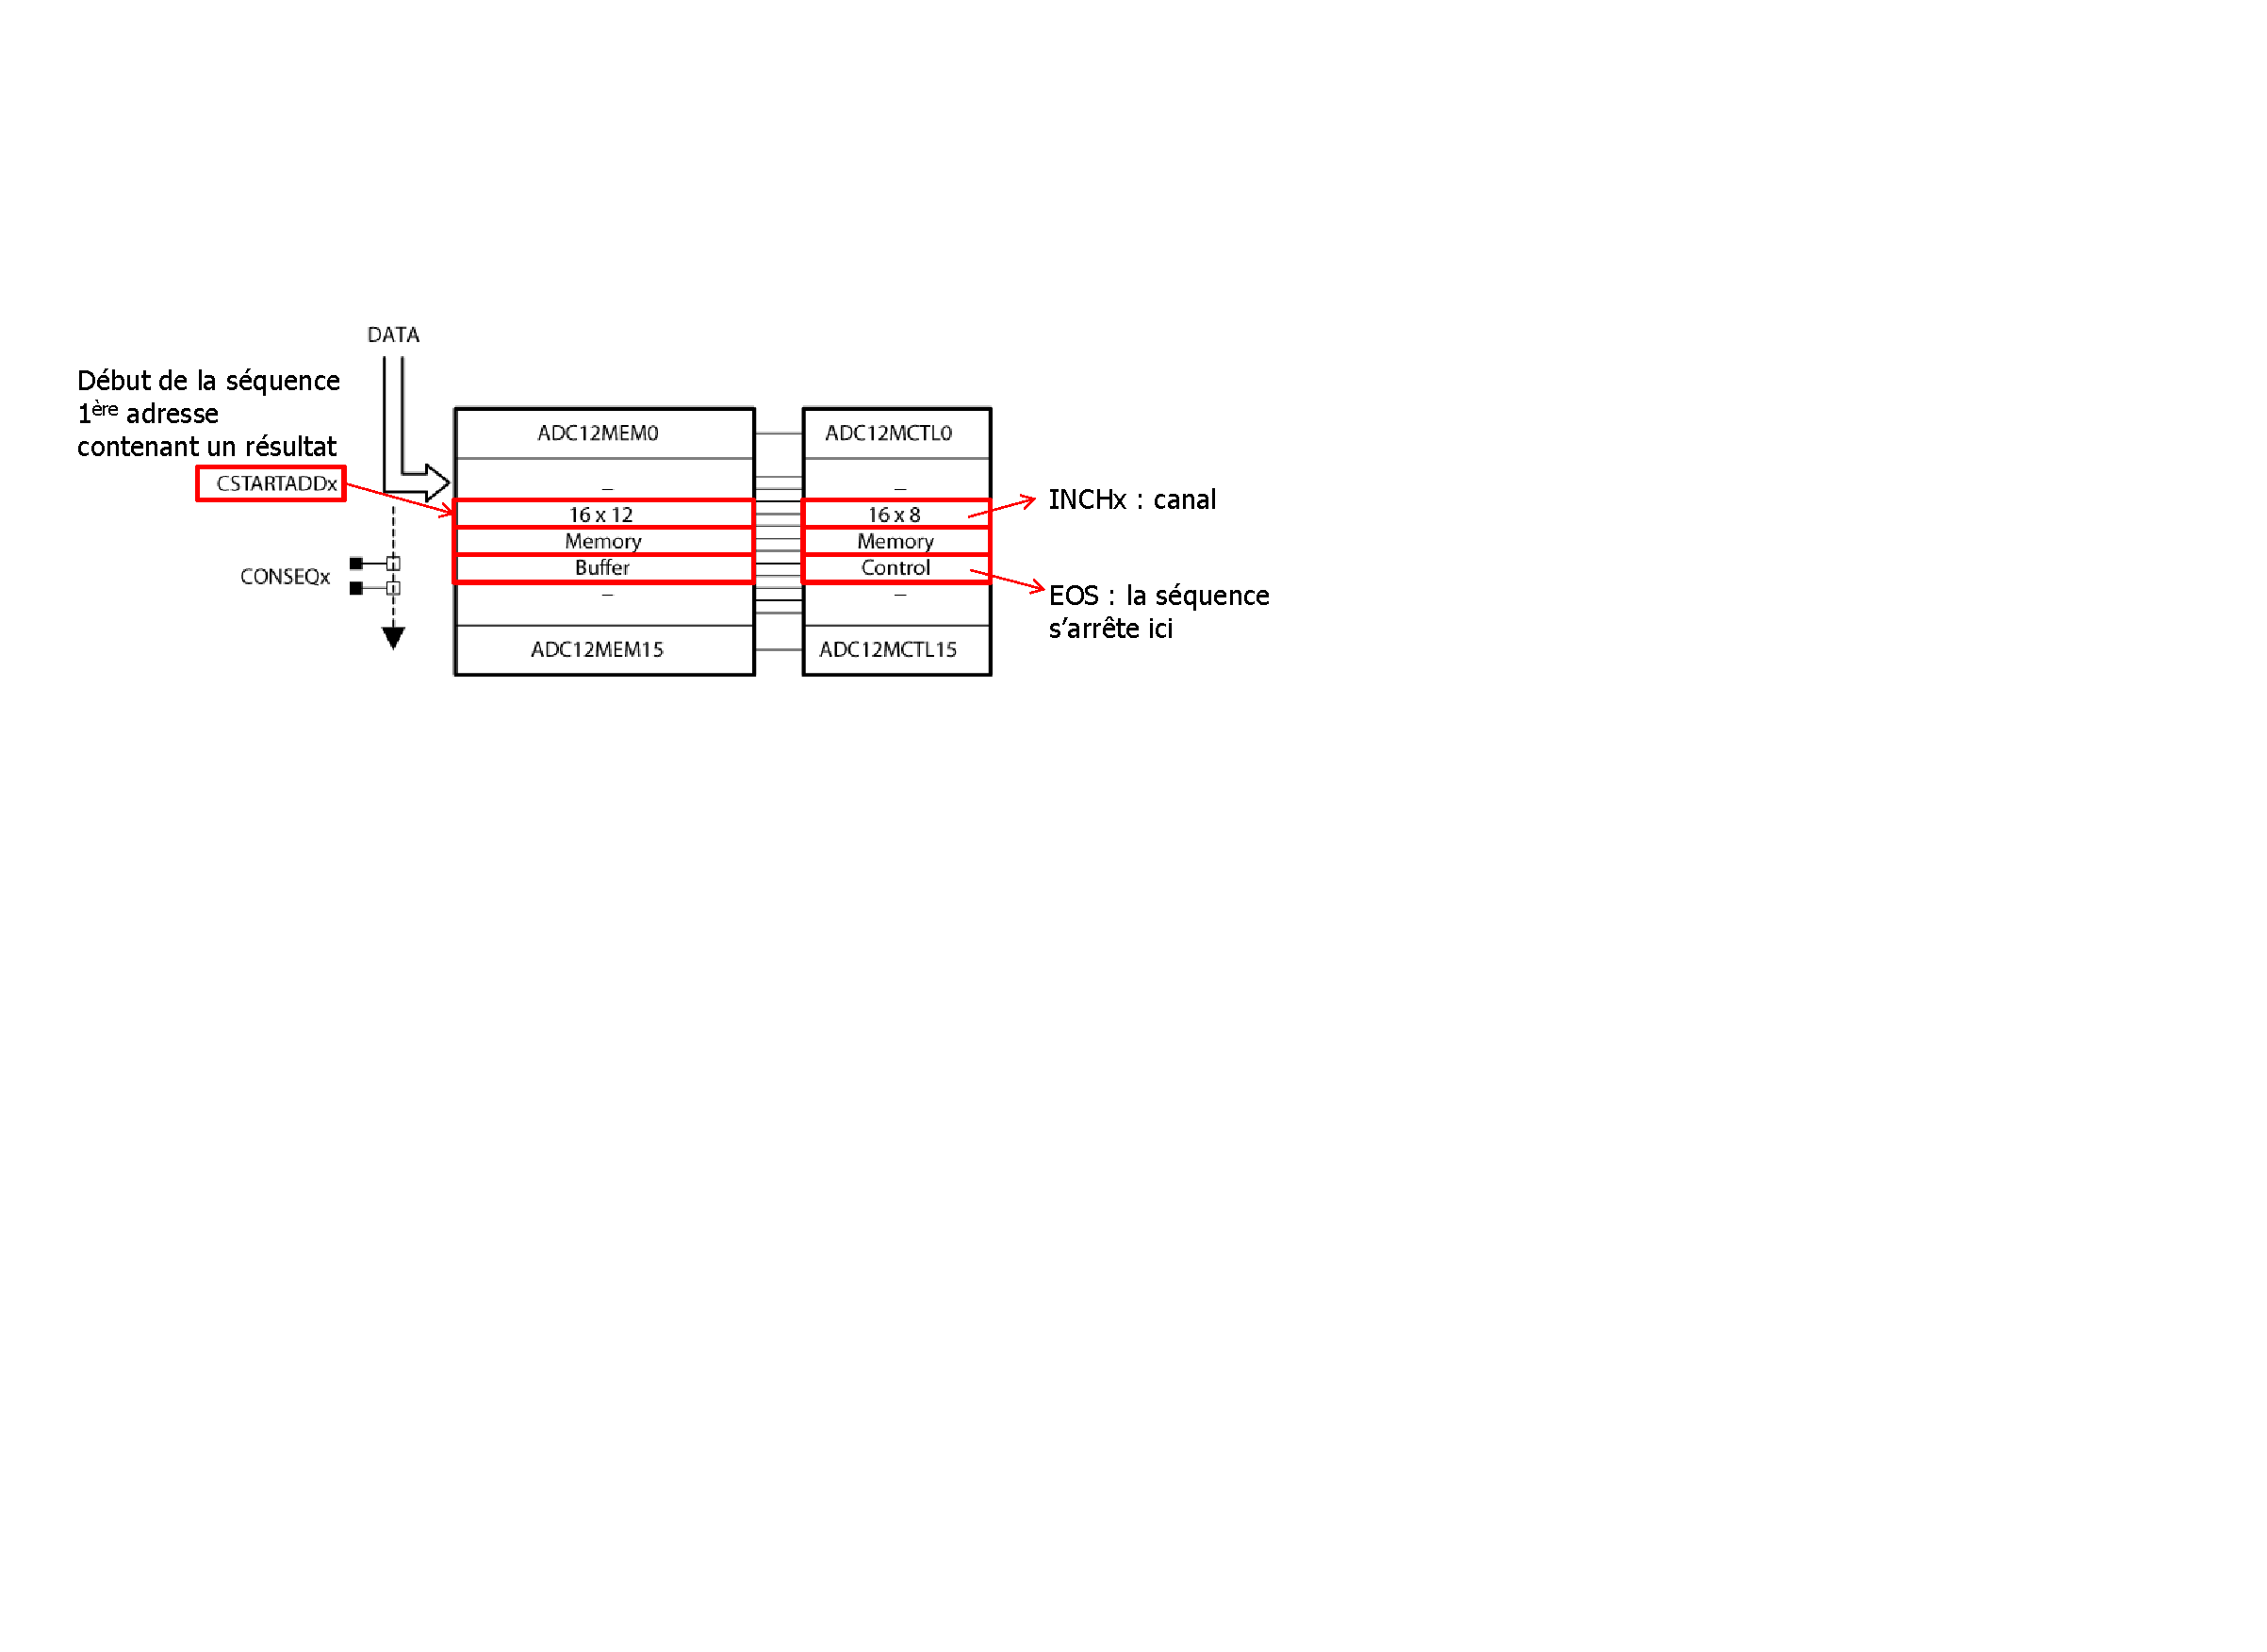
\includegraphics [angle=0, width=14cm]{./Figures/Chap11_ADC/ADC12Stockage.pdf}
  \rule{35em}{0.5pt}
  \caption{Organisation des registres de stockage et leur contr�le}
  \label{fig:ADC12Stockage}
\end{figure}

Un champ not� ADC12CSTARTADDx contient l'adresse du registre dans lequel se trouvera le r�sultat de la conversion. SI plusieurs conversions doivent �tre encha�n�es, ce champ indique dans quel registre se trouve le premier r�sultat, les autres se trouvant dans les registres ADC12MEMx suivants.
Pour contr�ler les conversions, chaque registre ADC12MCTLx contient 3 champs :
\begin{itemize}[label=\textbullet,font=\small]
\item INCHx : le num�ro de l'entr�e � convertir;
\item SREFx : le jeu de tensions de r�f�rence � utiliser;
\item EOS : le registre ADC12MCTLy contenant ce bit � '1' marque la fin de la s�quence.
\end{itemize}

Ainsi, chaque conversion d'une s�quence dispose de ses param�tres propres. Il est bien entendu possible de convertir le signal d'une seule entr�e, auquel cas il s'agit d'une s�quence d'une seule conversion.\\

Lors de l'�criture d'un r�sultat de conversion dans un registre, une requ�te d'interruption est �mise. Dans le cas d'une s�quence de conversions, il suffit de n'autoriser que celle correspondant � la fin de la s�quence.

\subsection{Registres de contr�le du convertisseur ADC12}

Ils sont nomm�s ADC12CTLx et sont au nombre de 3. Dans les tableaux suivants, on donne uniquement la signification des champs de contr�le les plus importants.

\begin{figure}[H]
  \centering
  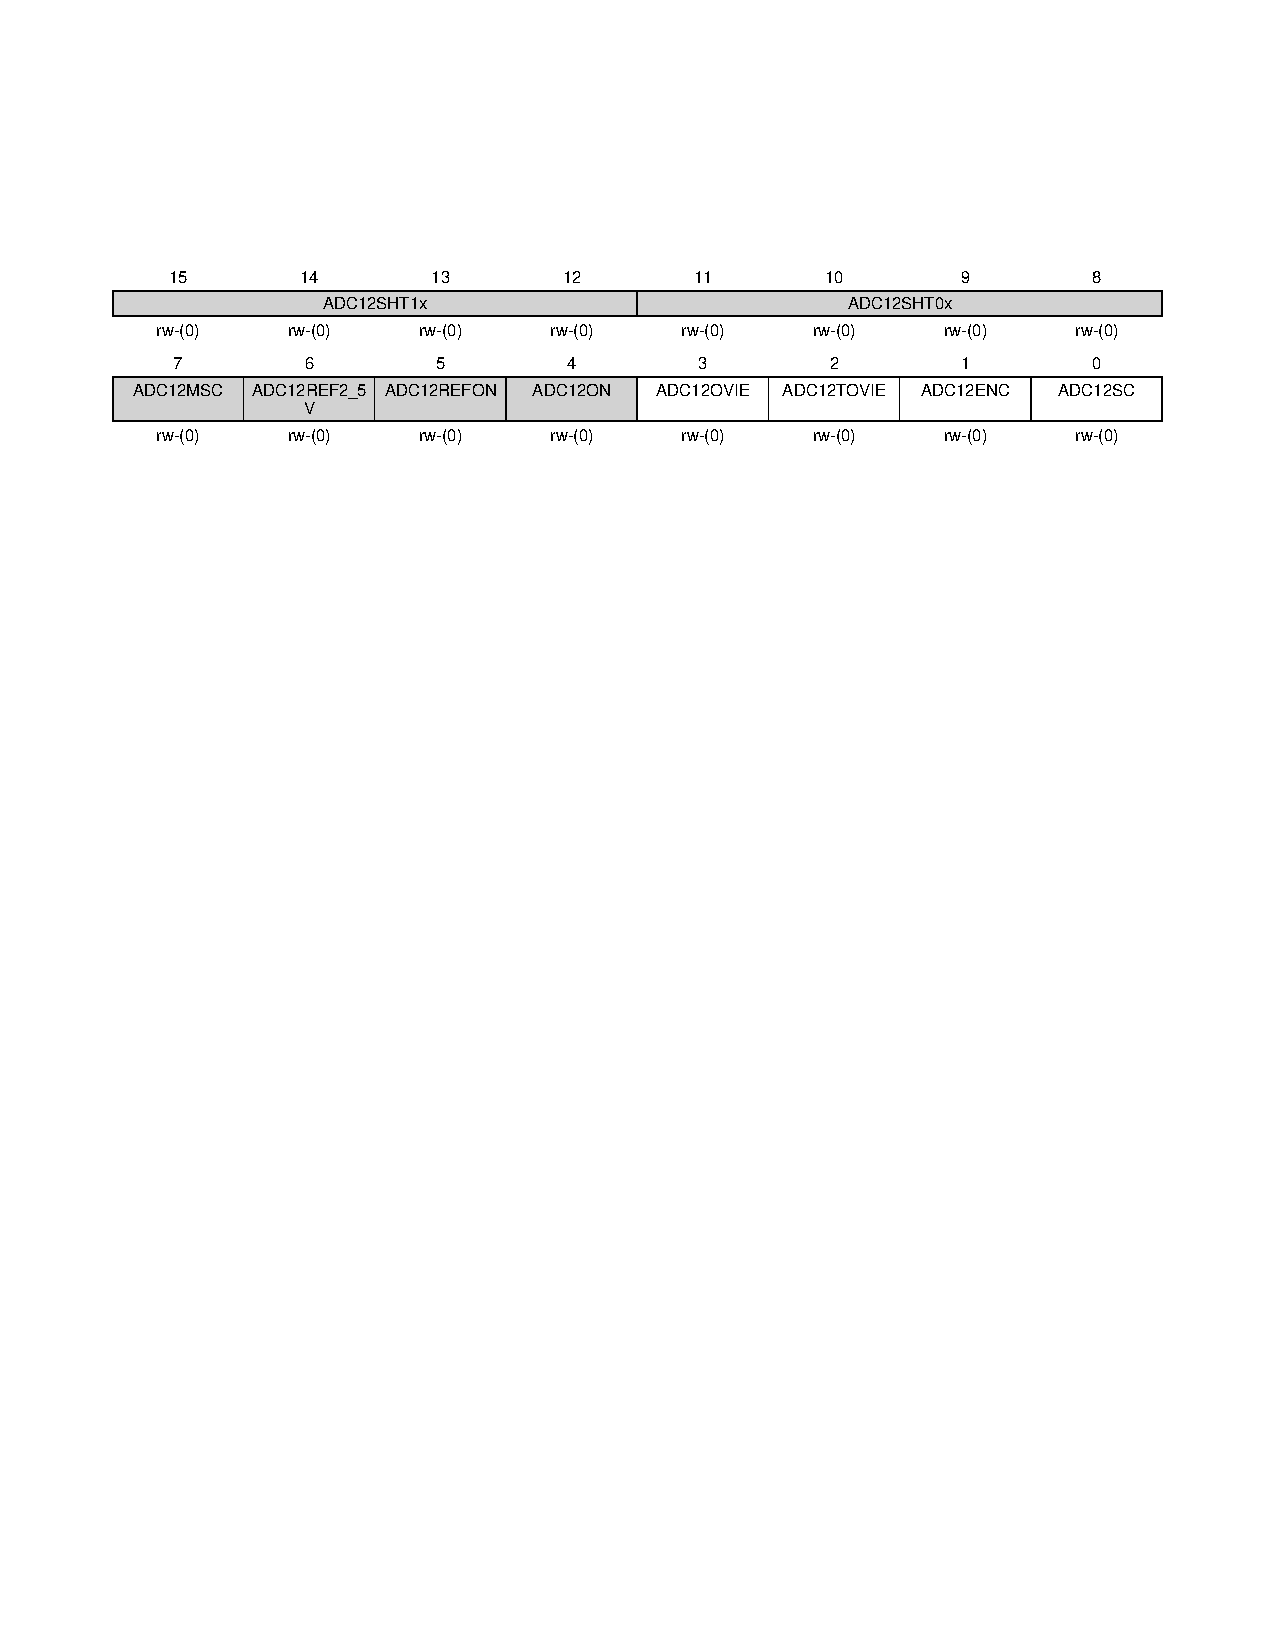
\includegraphics [angle=0, width=16cm]{./Figures/Chap11_ADC/ADC12CTL0.pdf}
  \rule{35em}{0.5pt}
  \caption{ADC12CTL0}
  \label{fig:ADC12CTL0}
\end{figure}

\begin{table}[H]
\centering 
\begin{tabular}{l l l l}
\hline\hline
Champ & & Valeur & Description \\ %[0.5ex]
\hline
ADC12SHT1 & & & Dur�e d'�chantillonnage pour les conversions \\
& & & contr�l�es par ADC12MCTL8 � ADC12MCTL15   \\
\hline
ADC12SHT0 & & & Dur�e d'�chantillonnage pour les conversions \\
& & &  contr�l�es par ADC12MCTL0 � ADC12MCTL7   \\
& & 0000b & 4 cycles de ADC12CLK \\
& & 0001b & 8 cycles de ADC12CLK \\
& & 0010b & 16 cycles de ADC12CLK \\
& & 0011b & 32 cycles de ADC12CLK \\
& & 0100b & 64 cycles de ADC12CLK \\
& & 0101b & 96 cycles de ADC12CLK \\
& & 0110b & 128 cycles de ADC12CLK \\
& & 0111b & 192 cycles de ADC12CLK \\
& & 1000b & 256 cycles de ADC12CLK \\
& & 1001b & 384 cycles de ADC12CLK \\
& & 1010b & 512 cycles de ADC12CLK \\
& & 1011b & 768 cycles de ADC12CLK \\
& & 11xxb & 1024 cycles de ADC12CLK \\
\hline
ADC12MSC & & - & Permet d'encha�ner des conversions multiples \\
\hline
ADC12ON & & - & Mise en marche du convertisseur \\
& & 0 & Convertisseur arr�t� \\
& & 1 & Convertisseur en marche \\
\hline
ADC12ENC & & - & Lancement du contr�leur de conversions \\
& & 0 & Contr�leur arr�t� \\
& & 1 & Contr�leur pr�t \\
\hline
ADC12SC & & - & Lancement d'une conversion \\
& & 1 & Start \\
\hline
\end{tabular}
\caption{ADC12CTL0}
\label{table:ADC12CTL0}
\end{table}

\pagebreak
\begin{figure}[H]
  \centering
  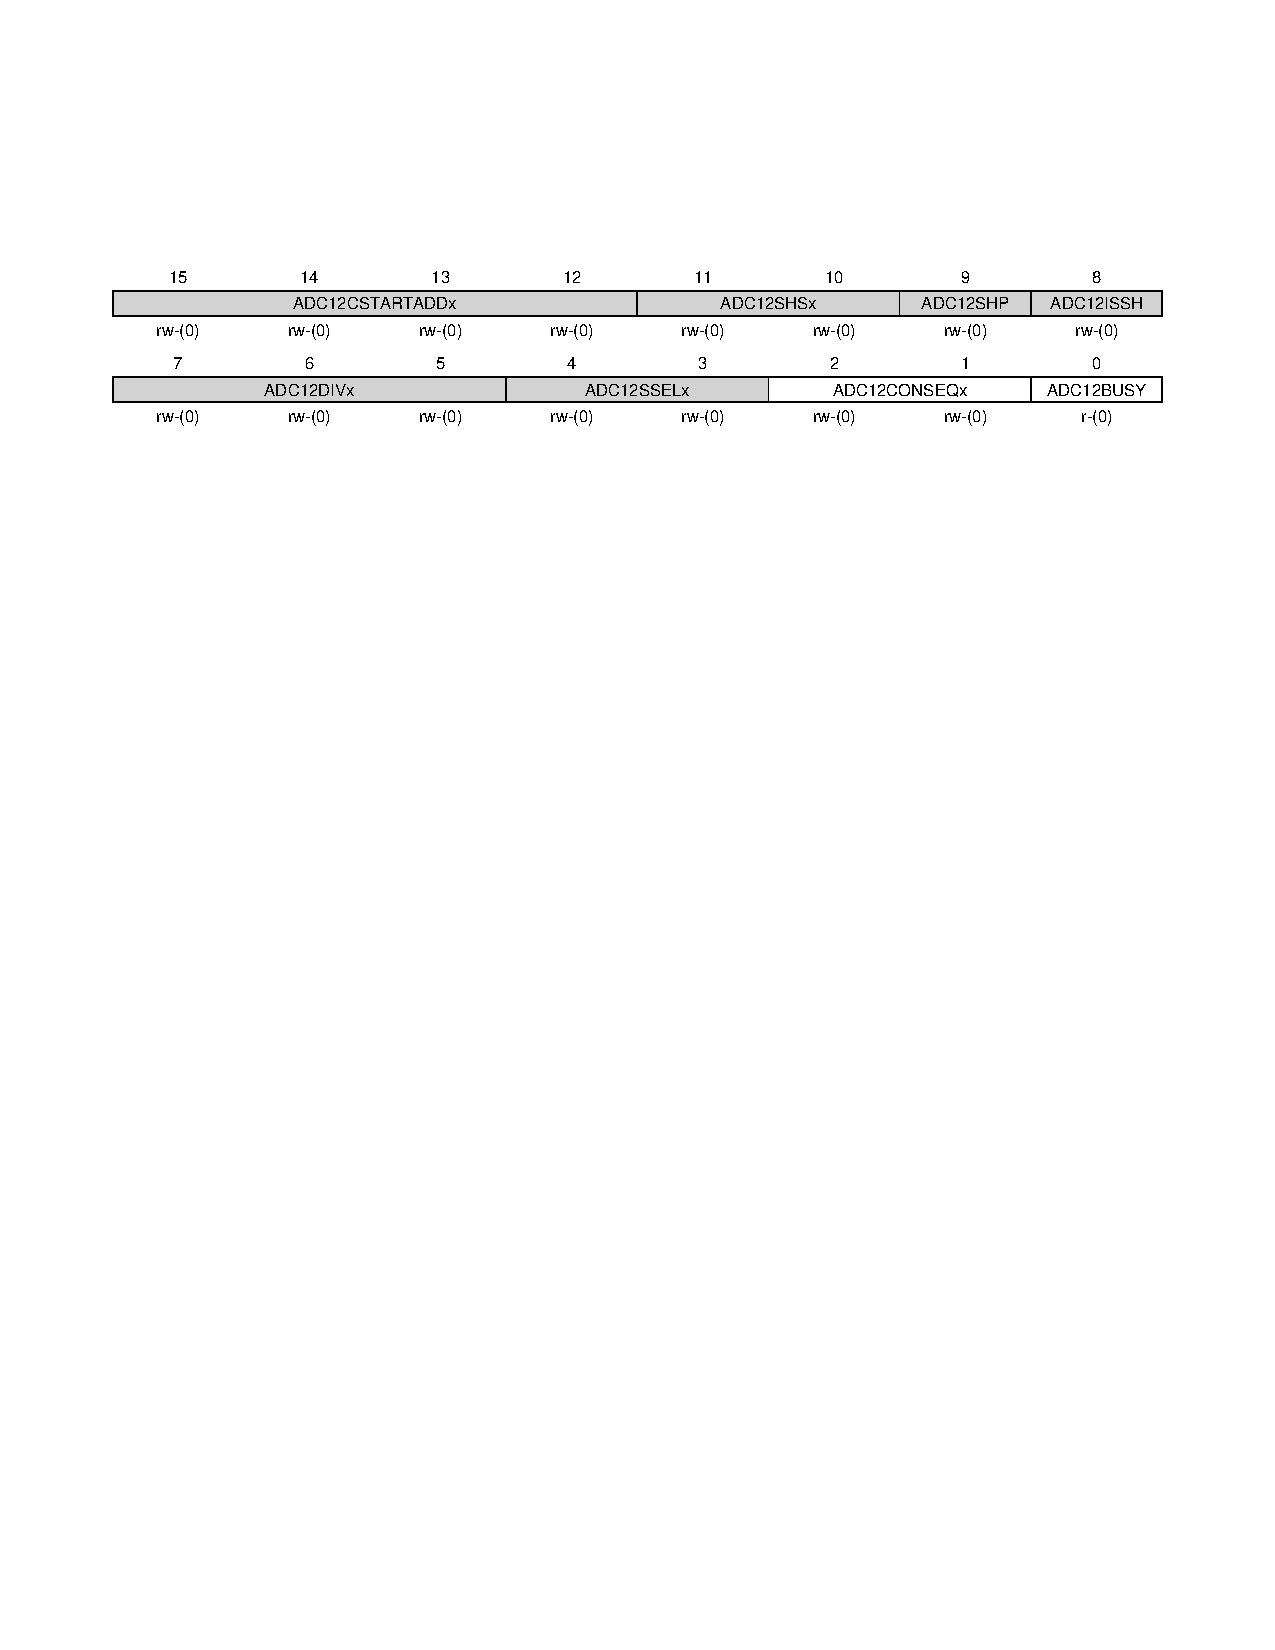
\includegraphics [angle=0, width=16cm]{./Figures/Chap11_ADC/ADC12CTL1.pdf}
  \rule{35em}{0.5pt}
  \caption{ADC12CTL1}
  \label{fig:ADC12CTL1}
\end{figure}

\begin{table}[H]
\centering 
\begin{tabular}{l l l l}
\hline\hline
Champ & & Valeur & Description \\ %[0.5ex]
\hline
ADC12CSTARTADD & & - & Adresse du registre de contr�le de la conversion \\
& & & ou de la premi�re conversion, dans le cas d'une s�quence \\
\hline
ADC12SHS & & & S�lection du signal de conversion \\
& & 00b & bit ADC12SC (lancement par logiciel) \\
& & 01b & timer (consulter la fiche technique du MCU) \\
& & 10b & timer (consulter la fiche technique du MCU) \\
& & 11b & timer (consulter la fiche technique du MCU) \\
\hline
ADC12SHP & & & Contr�le de la dur�e d'�chantillonnage \\
& & 0 & SAMPCON �gale le signal de conversion \\
& & 1 & Le niveau haut de SAMPCON est fix� par le timer de conversion \\
& & & voir le champ ADC12SHT0 ou ADC12SHT1 dans ADC12CTL0 \\
\hline
ADC12ISSH & & - & Inversion du signal de conversion (\ref{fig:ADC_Schema})\\
& & 0 & Pas d'inversion \\
& & 1 & Inversion \\
\hline
ADC12DIV & & - & Pr�division de l'horloge de conversion ADC12CLK \\
& & 000b & Division par 1 \\
& & 001b & Division par 2 \\
& & 010b & Division par 3 \\
& & 011b & Division par 4 \\
& & 100b & Division par 5 \\
& & 101b & Division par 6 \\
& & 110b & Division par 7 \\
& & 111b & Division par 8 \\
\hline
ADC12SSEL & & - & S�lection de l'horloge de conversion ADC12CLK \\
& & 00b & ADC12OSC \\
& & 01b & ACLK \\
& & 10b & MCLK \\
& & 11b & SMCLK \\
\hline
ADC12CONSEQ & & - & Mode de conversion \\
& & 00b & Conversion unique sur un canal unique \\
& & 01b & S�quence de conversions \\
& & 10b & Canal unique en r�p�tition \\
& & 11b & S�quence en r�p�tition \\
\hline
ADC12BUSY & & - & Indicateur de conversion en cours\\
& & 0 & Pas de conversion en cours \\
& & 1 & Une conversion en cours \\
\hline
\end{tabular}
\caption{ADC12CTL1}
\label{table:ADC12CTL1}
\end{table}

\pagebreak
\begin{figure}[H]
  \centering
  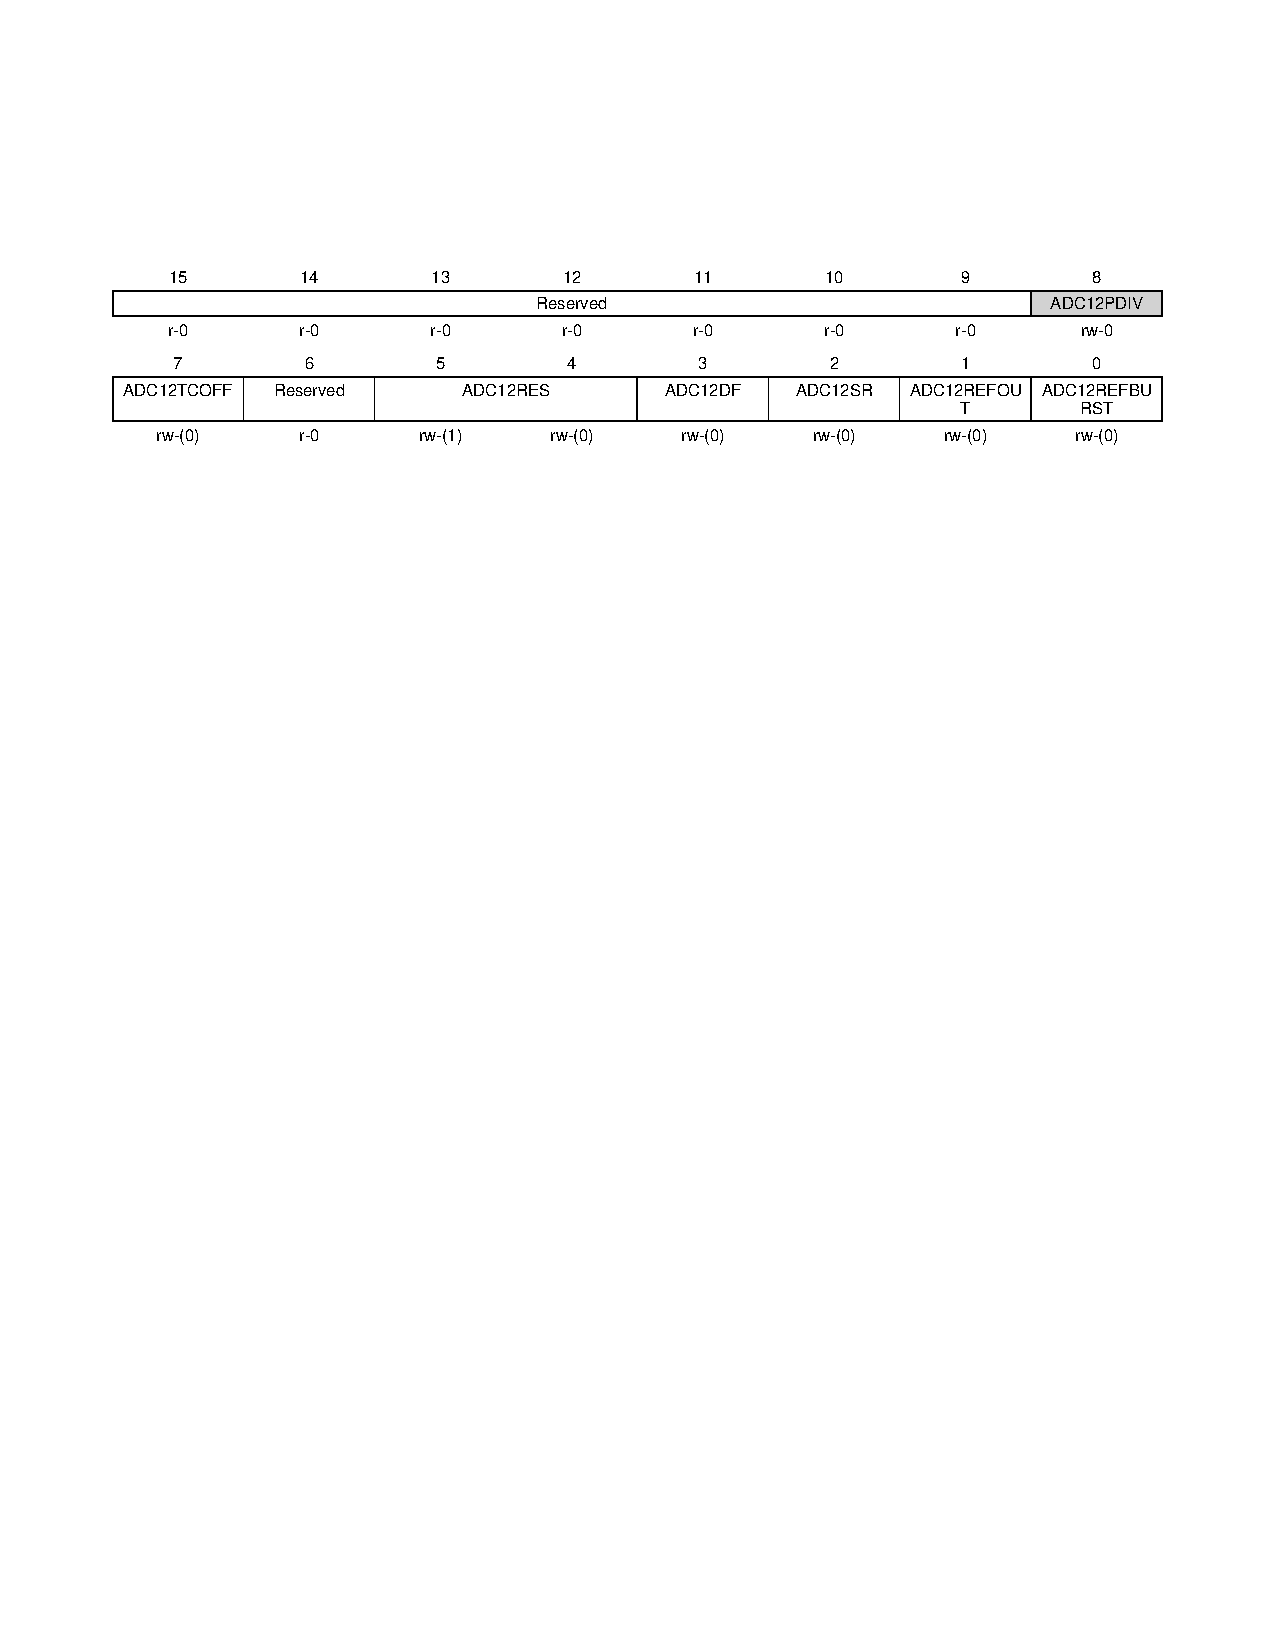
\includegraphics [angle=0, width=16cm]{./Figures/Chap11_ADC/ADC12CTL2.pdf}
  \rule{35em}{0.5pt}
  \caption{ADC12CTL2}
  \label{fig:ADC12CTL2}
\end{figure}

\begin{table}[H]
\centering 
\begin{tabular}{l l l l}
\hline\hline
Champ & & Valeur & Description \\ %[0.5ex]
\hline
ADC12CSTARTADD & & - & Adresse du registre de contr�le de la conversion \\
& & & ou de la premi�re conversion, dans le cas d'une s�quence \\
\hline
ADC12SHS & & & S�lection du signal de conversion \\
& & 00b & bit ADC12SC (lancement par logiciel) \\
& & 01b & timer (consulter la fiche technique du MCU) \\
& & 10b & timer (consulter la fiche technique du MCU) \\
& & 11b & timer (consulter la fiche technique du MCU) \\
\hline
ADC12SHP & & & Contr�le de la dur�e d'�chantillonnage \\
& & 0 & SAMPCON �agle le signal de conversion \\
& & 1 & Le niveau haut de SAMPCON est fix� par le timer de conversion \\
& & & voir le champ ADC12SHT0 ou ADC12SHT1 dans ADC12CTL0 \\
\hline
ADC12ISSH & & - & Inversion du signal de conversion (\ref{fig:ADC_Schema})\\
& & 0 & Pas d'inversion \\
& & 1 & Inversion \\
\hline
ADC12DIV & & - & Pr�division de l'horloge de conversion ADC12CLK \\
& & 000b & Division par 1 \\
& & 001b & Division par 2 \\
& & 010b & Division par 3 \\
& & 011b & Division par 4 \\
& & 100b & Division par 5 \\
& & 101b & Division par 6 \\
& & 110b & Division par 7 \\
& & 111b & Division par 8 \\
\hline
ADC12SSEL & & - & S�lection de l'horloge de conversion ADC12CLK \\
& & 00b & ADC12OSC \\
& & 01b & ACLK \\
& & 10b & MCLK \\
& & 11b & SMCLK \\
\hline
ADC12CONSEQ & & - & Mode de conversion \\
& & 00b & Conversion unique sur un canal unique \\
& & 01b & S�quence de conversions \\
& & 10b & Canal unique en r�p�tition \\
& & 11b & S�quence en r�p�tition \\
\hline
ADC12BUSY & & - & Indicateur de conversion en cours\\
& & 0 & Pas de conversion en cours \\
& & 1 & Une conversion en cours \\
\hline
\end{tabular}
\caption{ADC12CTL2}
\label{table:ADC12CTL2}
\end{table}


\appendix

\chapter{\textsc{Démonstrations algébriques}}
\label{ch:algebra}

De manière générale, on peut écrire un nombre entier non-signé sous la forme suivante:
\begin{equation}
\begin{aligned}
A_{10} &= \sum_{i=0}^{n-1} a_{i}2^{i} = a_{n-1}2^{n-1} + a_{n-2}2^{n-2} +...+ a_{1}2^{1} + a_{0}2^{0} \\
avec &:  a_{i} \in \{0,1\} \\
et &:   A_{10} \in [0...2^{n} - 1]
\end{aligned}
\end{equation}

Un nombre entier signé, en complément à deux, peut être écrit sous cette forme:
\begin{equation}
A_{10} = -a_{n-1}2^{n-1} + \sum_{i=0}^{n-2} a_{i}2^{i} = -a_{n-1}2^{n-1} + a_{n-2}2^{n-2} +...+ a_{1}2^{1} + a_{0}2^{0}
\end{equation}

\section{Changement de signe}

\begin{equation}
\begin{aligned}
-A_{10} &= \enspace - \Bigg( \underbrace{ -a_{n-1}2^{n-1} + \sum_{i=0}^{n-2} a_{i}2^{i}}_{A_{10}} \Bigg) \enspace = \enspace \underbrace{-2^{n-1} + \underbrace{\sum_{i=0}^{n-2} 2^{i} + 1}_{2^{n-1}}}_{0} + a_{n-1}2^{n-1} - \sum_{i=0}^{n-2} a_{i}2^{i} \\ &= \enspace -(1-a_{n-1})2^{n-1} + \sum_{i=0}^{n-2}(1-a_i)2^i + 1 \enspace = \enspace -\bar{a}_{n-1}2^{n-1} + \sum_{i=0}^{n-2} \bar{a}_{i}2^{i} + 1 \\ &= \enspace \bar{A} + 1
\end{aligned}
\end{equation}

\section{Extension d'un nombre signé}

On cherche à trouver les bits $b_i$ qui permettent d'étendre un nombre négatif ($a_{n-1}=1$) en complément à deux de n bits à m bits:
\[ a_{n-1} a_{n-2} ... a_{0} \Rightarrow b_{m-1} b_{m-2} ... b_{n-1} a_{n-2} ... a_{0} \]

Exemple:
\[m =8, n=4: a_3 a_2 a_1 a_0 = b_7 b_6 b_5 b_4 b_3 a_2 a_1 a_0 \]
Avec $a_3$ le bit de signe original et $b_7$ le bit de signe du nombre étendu. $a_3$ se déplace donc en première position $b_7$ pour conserver le bit de signe. Comme ils valent 1 on les simplifies et la notation peut s'écrire de manière générale:

\begin{equation}
\begin{aligned}
-2^{n-1} + \sum_{i=0}^{n-2}a_i 2^i \enspace &= \enspace -2^{m-1} + \sum_{i=n-1}^{m-2} b_{i}2^{i} + \sum_{i=0}^{n-2}a_i 2^i  \quad m > n\\
-2^{n-1} \enspace &= \enspace -2^{m-1} + \sum_{i=n-1}^{m-2} b_{i}2^{i} \\
2^{m-1} \enspace &= \enspace 2^{n-1} + \sum_{i=n-1}^{m-2} b_{i}2^{i}
\end{aligned}
\end{equation}

Cette égalité est toujours vraie si est seulement si les $b_i$ sont égaux à 1 et quelque soit m, n (m > n). Exemples:
\[
m=4, n=2: \quad 2^{4-1} = 2^{2-1} + b_1 2^{1} + b_2 2^{2} \Leftrightarrow 8 = 2 + 1 \cdot 2 + 1 \cdot 4
\]

\[
m=8, n=4: \quad 2^{8-1} = 2^{4-1} + b_3 2^{3} + b_4 2^{4} + b_5 2^{5} + b_6 2^{6}\Leftrightarrow 128 = 8 + 1 \cdot 8 + 1 \cdot 16 + 1 \cdot 32 + 1 \cdot 64
\]

\section{Multiplication de nombres en complément à deux}
La multiplication en colonnes classique fonctionne en complément à 2 mais elle nécessite une correction à la fin du calcul en fonction du signe des opérandes pour retrouver le résultat correct. Soit m et r, deux entier sur n bits:

\begin{equation}
\begin{aligned}
+m \equiv m \enspace & \enspace +r \equiv r\\
-m \equiv 2^n-m \enspace & \enspace -r \equiv 2^n-r\\
(+m) \times (+r) \enspace &= \enspace mr\\
(-m) \times (+r) \enspace &= \enspace 2^{n}r - mr\\
(+m) \times (-r) \enspace &= \enspace 2^{n}m - mr\\
(-m) \times (-r) \enspace &= \enspace 2^{n}2^{n} - 2^{n}m - 2^{n}r + rm
\end{aligned}
\end{equation}

Le facteur $2^{n}2^{n}$ disparait par arithmétique modulo. Il reste néanmoins une correction à effectuer qui est différente pour chaque cas. Cette différence de temps de calcul en fonction du signe est gênante mais peut être évitée grâce à l'algorithme de Booth (1950) \cite{booth}. L'algorithme consiste en la transformation suivante:

\begin{equation}
\begin{aligned}
A \cdot B &= \enspace B \Bigg( \underbrace{ -a_{n-1}2^{n-1} + \sum_{i=0}^{n-2} a_{i}2^{i}}_{A_{10}} \Bigg) \enspace 
= \enspace  B \Bigg( -a_{n-1}2^{n-1} + 2\sum_{i=0}^{n-2} a_{i}2^{i} - \sum_{i=0}^{n-2} a_{i}2^{i} \Bigg) \\ 
&= \enspace B \Bigg( -a_{n-1}2^{n-1} + \sum_{i=0}^{n-2} a_{i}2^{i+1} - \sum_{i=0}^{n-2} a_{i}2^{i} \Bigg) \enspace 
= \enspace B \Bigg( \sum_{i=1}^{n-1} a_{i-1}2^{i} - \sum_{i=0}^{n-1} a_{i}2^{i} \Bigg) \\ 
&= \enspace B \Bigg( \sum_{i=1}^{n-1} (a_{i-1}-a_i)2^{i} - a_{0}2^{0} \Bigg)
\end{aligned}
\end{equation}

Et comme le terme $a_{-1}$ peut être considéré nul car en dehors du nombre alors:

\begin{equation}
A \cdot B = \enspace \sum_{i=0}^{n-1} B(a_{i-1}-a_i)2^{i}
\end{equation}

On peut montrer numériquement que le résultat de la multiplication est correct indépendamment du signe de A et de B \cite{booth}.

L'algorithme de Booth peut être étendu pour inclure des séquences de "1" grâce à la même propriété utilisée ci-dessus qui est que tout "1" logique peut s'écrire $a_i2^i = a_i2^{i+1}-a_i2^i$ et donc toute séquence de "1" peut s'écrire $a_i2^{i+k}-a_i2^i$ (avec k la longueur de la séquence de 1). Ceci permet de réduire le nombre de multiplications à effectuer. Prenons un exemple pour bien comprendre:
\[
A \cdot B = A \cdot "00111110" = A \cdot (2^5 + 2^4 + 2^3 + 2^2 + 2^1) = A \cdot 62
\]
\[
A \cdot B = A \cdot "00111110" = A \cdot (2^6 - 2^1) = A \cdot (64 - 2)
\]
On passe donc de 5 à 2 termes à calculer.

La réalisation de cet algorithme est simplifiée si on parcours le multiplicateur de gauche à droite en faisant une addition du multiplicande lorsqu'on rencontre "01" (début de séquence) et une soustraction du multiplicande lorsqu'on rencontre "10" (fin de séquence) avec les décalages appropriés. On peut aussi le faire dans l'autre sens avec début à "10" et fin à "01".
Cet algorithme peut être encore étendu en utilisant le concept du codage redondant. Par exemple pour le cas ci-dessus on considère deux bits à chaque itération. On peut aussi en considérer trois ou même quatre à chaque itération ce qui donne plus de flexibilité pour coder avantageusement le multiplicateur.

\begin{thebibliography}{1}

\bibitem[1]{booth}Andrew D. Booth, \emph{A Signed Binary Multiplication Technique}, Journal of Mechanical and Applied Mathematics, 1951
%
%\bibitem[2]{proakis}John G. Proakis, Dimitris G. Manolakis: \emph{Digital Signal Processing}, Pearson Prentice Hall, 2007
%
\end{thebibliography}   %TBD

%\bigskip
\end{document}